\chapter{Modeling}
\label{sec:modeling}
Multirotor flight position control essentially boils down to tilting the vehicle into the desired direction. Our position control therefore must find a reference attitude and thrust that makes the MAV move to the targeted positions. This reference attitude and thrust must be translated into reference motor rates by some attitude control. 

In this project we split these two tasks task by the means of a cascaded control approach (see figure \ref{pics:controller_sketch}). We will run the dynamically faster attitude and motor control at a high rate ($1000 \si{\hertz}$) in an inner loop and the high level position controller at $100 \si{\hertz}$ in an outer loop. 
\begin{figure}
\centering
\includegraphics{images/controller_sketch.tikz}
\caption{Cascaded control sketch}
\label{pics:controller_sketch}
\end{figure}

It simplifies the design of the position controller as only translational dynamics have to be considered explicitly and position control reduces to controlling the vehicles desired thrust and direction. 

In order for the vehicle to move to a reference position, the position controller computes the desired thrust force and roll, pitch, yaw angles. The inner loop then takes care of finding the appropriate moment applied to the vehicle body to archive the desired attitude. In this section the components from the control scheme in figure \ref{pics:controller_sketch} are modeled. 


First the multirotor platform is described. Then a compilation of models is derived to build the complete model. It starts with a detailed model on the equations of motion (section \ref{sec:eq_of_motion}), which explicitly contain the influence of motor drag. Next a model for wind and wind forces is proposed (section \ref{sec:wind_model}). In section \ref{sec:sys_id} the attitude dynamics are evaluated through system identification. Finally all these models are summarized into a set of overall dynamics which will describe our control system.

%%%%%%%%%%%%%%%%%%%%%%%%%%%%%%%%%%%%%%%%%%%%%%%%%%%%%%%%%%%%%%%%%%%%%%%%%%%%%%%
% Platform
%%%%%%%%%%%%%%%%%%%%%%%%%%%%%%%%%%%%%%%%%%%%%%%%%%%%%%%%%%%%%%%%%%%%%%%%%%%%%%%
\section{Platform}
The AscTec Firefly (see figure \ref{pics:firefly}) is a hexacopter which is specifically designed for research purposes. While this is a hexacopter, the dynamics and controllers are generalized for any multirotor configuration. Here, a multirotor is a flying platform consisting of a body and a user specified arrangement of three or more rotors. Only configurations are considered which have all rotors lying fixed in a plane.

In platforms with even-numbered motors, neighboring rotors typically rotate in opposite direction. This compensates yaw moments and gives control over heading. Tilting is accomplished by increasing the thrust on on one side of the vehicle and decreasing it on the opposite side.

The Firefly has six $20 \si{\cm}$ diameter rotors equally aligned around the center. It is $60.5 \times 66.5 \times 16.5 \si{\cm}$ in size and weights $1.6 \si{\kg}$. The maximum thrust is $36 \si{\N}$ and it reaches a maximum airspeed of $15 \si{\metre\per\second}$.

\begin{figure}
   \centering
   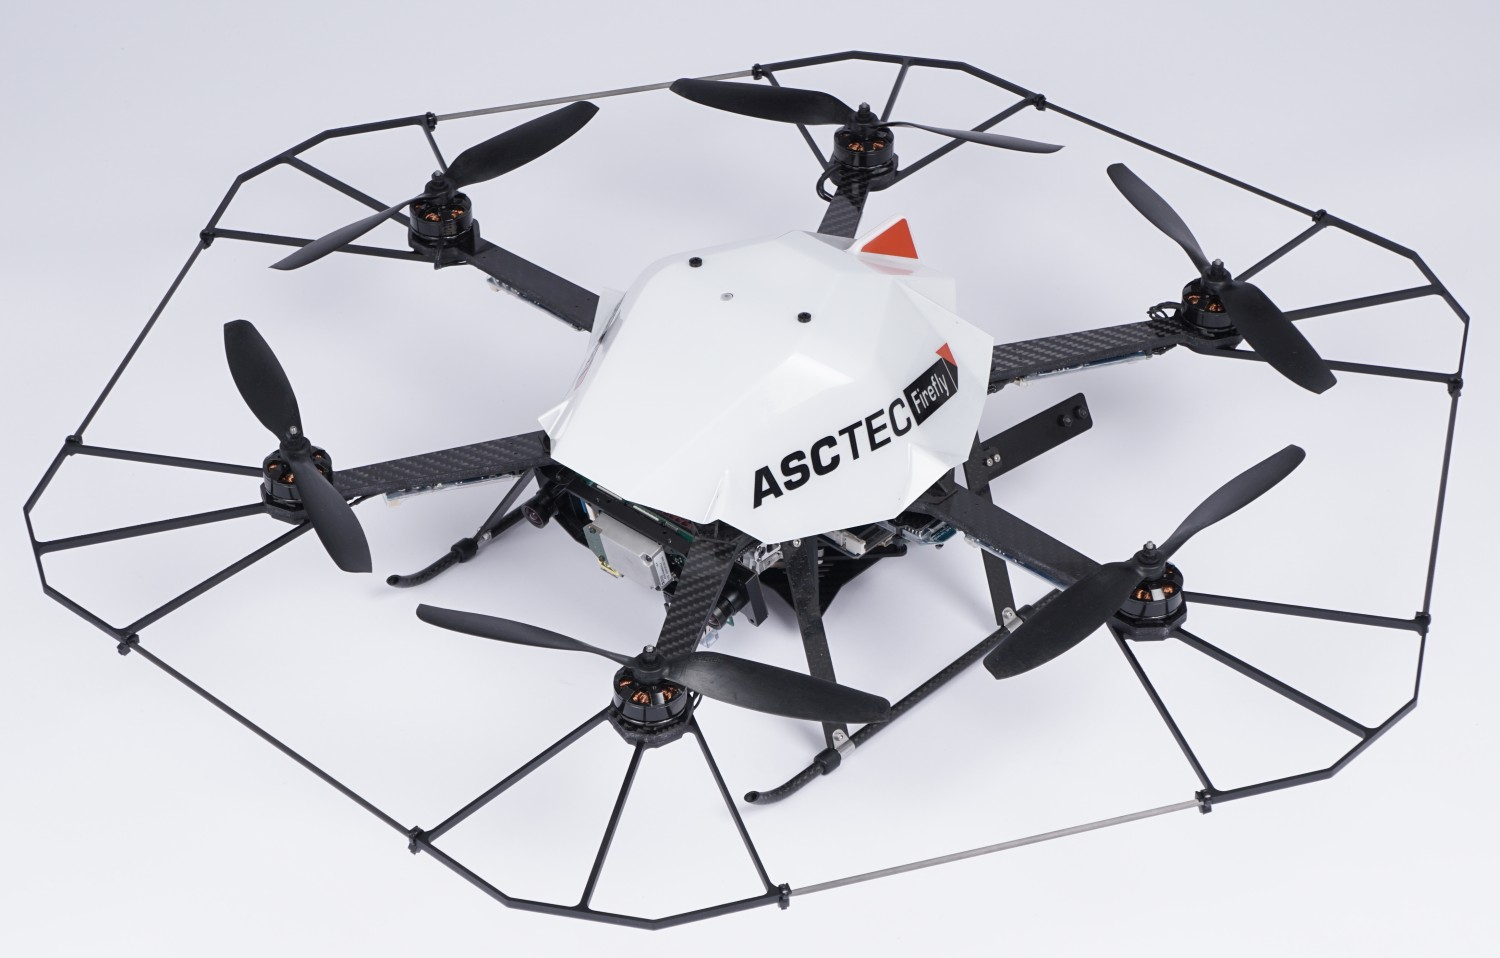
\includegraphics[width=0.75\textwidth]{images/firefly.jpg}
   \caption{AscTec Firefly \cite{www:asctec}}
   \label{pics:firefly}
\end{figure}

It is provided with an inertial measurement unit (IMU) and has a efficient attitude controller onboard. In the experiment an external optical motion capture system by Vicon is used to feedback precise position information. A processor is taking care of online computation.

%%%%%%%%%%%%%%%%%%%%%%%%%%%%%%%%%%%%%%%%%%%%%%%%%%%%%%%%%%%%%%%%%%%%%%%%%%%%%%%
% Equations of Motion
%%%%%%%%%%%%%%%%%%%%%%%%%%%%%%%%%%%%%%%%%%%%%%%%%%%%%%%%%%%%%%%%%%%%%%%%%%%%%%%
\section{Equations of Motion}
\label{sec:eq_of_motion}
The multirotor is modeled as a rigid body with six degrees of freedom (DoF). It has three translational DoF $x$, $y$, $z$ and three rotational DoF roll, pitch and yaw ($\phi$, $\theta$, $\psi$).

 For modeling purposes, we define proper reference frames and notations first. Then the dynamics acting at each rotor are stated. Next the Newton's and Euler's equations for the vehicle are formed giving the complete dynamics of the vehicle.

\subsection{Coordinate Systems and Notations}
\label{sec:coordinates}
\subsubsection{Coordinate Systems}
In total three main reference frames are defined. 
\begin{description}
\item[1. World-fixed frame] Cartesian coordinate system $\mathcal{W}$ with $x$, $y$, $z$ pointing east, north, up, and with the origin at the MAV's initial position.
\item[2. Orientation-fixed frame] Cartesian coordinate system $\mathcal{O}$ rotating world-fixed frame around the $z$-axis through the current heading of the MAV. 
\item[3. Body-fixed frame] Cartesian coordinate system $\mathcal{B}$ oriented along the multirotor's body axes $x$, $y$, $z$ pointing forward, sidewards left, upwards in direction of thrust, and having the origin at the center of gravity and body's principal axes of inertia.
\end{description}

\subsubsection{Notations}
We denote vectors and matrices with a bold letter. A trailing calligraphic subscript on a vector denotes the corresponding coordinate frame $\mathcal{W}$, $\mathcal{O}$ or $mathcal{B}$. 

In general, we will consider positions $\mathbf{r}$, velocities $\mathbf{v}$ and accelerations $\mathbf{a}$ in world-fixed coordinates, i.e.
\begin{align}
\mathbf{r} &= \begin{bmatrix}
x \\ y \\ z
\end{bmatrix},
& \mathbf{v} &= \begin{bmatrix}
\dot{x} \\ \dot{y} \\ \dot{z}
\end{bmatrix},
& \mathbf{a} &= \begin{bmatrix}
\ddot{x} \\ \ddot{y} \\ \ddot{z}
\end{bmatrix},
\end{align}
and omit the subscript. Rotational velocities $\boldsymbol{\omega}$ are considered in body-fixed coordinates.
\begin{align}
\boldsymbol{\omega} = \begin{bmatrix}
p \\ q \\ r
\end{bmatrix}
\end{align}

A calligraphic trailing double subscript on a matrix denotes the coordinate transformation from the second subscript frame to the first subscript frame. A single trailing subscript serves as additional descriptor. System matrices with a bar are denoted as the discrete time approximations, discretized about the position control sampling time $T_s = 0.01 \si{\second}$.

We abbreviate $\sin(\cdot)$ and $\cos(\cdot)$ with $s \cdot$ or $c \cdot$ respectively.

\subsubsection{Rotations}
For attitude representation we will use Euler angles $[\phi,~\theta,~\psi]$ following the $zyx$--sequence exclusively. The advantage of this representation is its simplicity and broad usage. However, it has three major disadvantages over unit quaternions. First, the proposed Euler angle sequence is prone to singularities at pitch angles $\theta = \frac{\pi}{2} + n\pi,~\forall~n\in\mathbb{Z}$. Second, they are less accurate when integrating incremental changes in attitude. Third, it is computational more expensive to evaluate trigonometric functions. Diebel provides a nice review on all sorts of transformations \cite{Diebel2006}. We will thus limit this report to introducing the necessary rotation matrices and assumptions made.

For a coordinate rotation about a single axis by an angle $\alpha$, we get the following rotation matrices from the special orthogonal group $SO(3)$:
\begin{align}
\mathbf{R}_x (\alpha)&=  \begin{bmatrix}
1 & 0 & 0 \\
0 & c\alpha & s\alpha \\
0 & -s\alpha & c\alpha
\end{bmatrix} ,\\
\mathbf{R}_y (\alpha)&=  \begin{bmatrix}
c\alpha & 0 & -s\alpha \\
0 & 1 & 0 \\
s\alpha & 0 & c\alpha
\end{bmatrix} ,\\
\mathbf{R}_z (\alpha)&=  \begin{bmatrix}
c\alpha & s\alpha & 0 \\
-s\alpha & c\alpha & 0 \\
0 & 0 &1
\end{bmatrix}.
\end{align}

The coordinate transformation from world-fixed frame $\mathcal{W}$ to orientation-fixed frame $\mathcal{O}$ is obtained by rotating the initial frame about the $z$--axis by the current heading $\psi$.
\begin{align}
\rotOW(\psi) = \mathbf{R}_z (\psi)
\end{align} 
The backwards transformation is achieved by transposition.
\begin{align}
\rotWO(\psi) = \rotOW^{-1}(\psi) = \rotOW^{T}(\psi)
\end{align}

Similar, the direction cosine matrix for the transformation from world-fixed frame $\mathcal{W}$ to body-fixed frame $\mathcal{B}$ is obtained. Following $xyz$--convention, we get
\begin{align}
\rotBW(\phi,\theta,\psi) &= {\mathbf{R}_x} (\phi) \cdot {\mathbf{R}_y} (\theta) \cdot {\mathbf{R}_z} (\psi) \\
&=
 \begin{bmatrix}
c\theta c\psi 				&c\theta s\psi 				& -s\theta  \\
s\phi s\theta c\psi - c\phi s\psi  	& s\phi s\theta s\psi + c\phi c\psi 	& s\phi c\theta \\
c\phi s\theta c\psi + s\phi s\psi	& c\phi s\theta s\psi - s\phi c\psi 	& c\phi c\theta
\end{bmatrix} ,\\
%
%
\rotWB (\phi,\theta,\psi) &= {\rotBW^{-1} (\phi,\theta,\psi)} = {\rotBW^{T} (\phi,\theta,\psi)} \\
&=
\begin{bmatrix}
c\theta c\psi & s\phi s\theta c\psi - c\phi s\psi & c\phi s\theta c\psi + s\phi s\psi \\
c\theta s\psi & s\phi s\theta s\psi + c\phi c\psi & c\phi s\theta s\psi - s\phi c\psi \\
-s\theta & s\phi c\theta & c\phi c\theta
\end{bmatrix}.
\end{align}

Finally, rotations from the orientation-fixed frame $\mathcal{O}$ to the body fixed frame $\mathcal{B}$ and reverse are
\begin{align}
\rotBO (\phi,\theta) &= {\mathbf{R}_x} (\phi) \cdot {\mathbf{R}_y} (\theta)  ,\\
\rotOB (\phi,\theta) &= {\rotBO^{-1} (\phi,\theta)} = {\rotBO^{T} (\phi,\theta)}.
\end{align}

In general, we will omit the attitude arguments in the rotation matrices.

\subsubsection{Connection Rotation Rates and Euler Rates}
To convert measured body rotation rates $\boldsymbol{\omega}$ into Euler angle rates we use the conjugate Euler angle rate matrix $\mathbf{E}_{xyz}'$.
\begin{align}
\begin{bmatrix}
\dot{\phi} \\ \dot{\theta} \\ \dot{\psi}
\end{bmatrix}
= [\mathbf{E}_{xyz}'(\phi,\theta,\psi)]^{-1} \cdot \boldsymbol{\omega} 
= \frac{1}{c\theta} \begin{bmatrix}
c\theta & s\phi s\theta & c\phi s\theta \\
0 & c\phi c\theta & -s\phi c\theta \\
0 & s\phi & c\phi
\end{bmatrix} \cdot \begin{bmatrix}
p \\ q \\ r
\end{bmatrix}
\end{align}

\subsection{Dynamics}
\label{sec:dynamics}
Martin et al. \cite{Martin2010} propose that the dominant forces and moments acting on a regular multirotor origin from the summation of the aerodynamic effects at each rotor and the gravitational force. We state the rotor dynamics with equations \ref{eq:rotor_begin} to \ref{eq:rotor_begin} which eventually lead to the Newton's equation \ref{eq:newton} and Euler's equation \ref{eq:euler} which completely describe the vehicle equations of motion. We do not model motor dynamics as they are much faster than the translational dynamics.

\subsubsection{Rotor Dynamics}
Blade theory gives the mechanics of each propeller/motor assembly. We neglect 
\begin{itemize} 
\item blade flapping (stiff rotors),
\item high order linear and angular velocity terms (small at hovering compared to blade tip speed),
\item linear and angular acceleration of propellers (low mass),
\item angular acceleration of motors (small at hovering),
\item friction torque due to rotational motion.
\end{itemize}

The remaining major forces are thrust $F_T$ and drag $F_D$. Thrust acts perpendicular to the blade plane and lifts the body. Drag acts opposing to the vehicle's airspeed and slows down the vehicle. The major torques acting on a single blade are roll moments $M_R$ and drag moments $M_D$. The direction of these moments and forces are depicted in figure. 

\begin{align}
\mathbf{F}_T&= \omega^2 \cdot C_T \cdot \mathbf{e}_{\mathcal{B},z}  &\text{(thrust)} ,\label{eq:rotor_begin} \\
\mathbf{F}_D&= -\omega \cdot  C_D \cdot \body{\mathbf{\boldsymbol{\nu}}^\perp} &\text{(drag)} , \label{eq:drag_force}\\
\mathbf{M}_R&= \omega \cdot C_R \cdot \body{\mathbf{\boldsymbol{\nu}}^\perp} &\text{(roll)} , \\
\mathbf{M}_D&= -\epsilon \cdot C_M \cdot \mathbf{F_T}  &\text{(drag)}, \label{eq:rotor_end}
\end{align}
where
\begin{align*}
\omega &: &\text{angular velocity of rotor blade}, \\
C_T>0 &: &\text{thrust constant}, \\
C_D>0 &: &\text{drag constant}, \\
C_R>0 &: &\text{rolling moment constant}, \\
C_M>0 &: &\text{drag moment constant}, \\
\epsilon\in\{-1,1\} &: &\text{turning direction (clockwise, counter clockwise)}, \\
\mathbf{e}_{\mathcal{B},z} &: &\text{unit vector in z-direction in base coordinates},\\
\body{\mathbf{\boldsymbol{\nu}}} &: &\text{airspeed in base coordinates} .
\end{align*}

The $\perp$-symbol denotes the projection of the air speed on the propeller plane (see figure). It can be calculated as:

\begin{align}
\body{\mathbf{\boldsymbol{\nu}}^\perp} &= \mathbf{e}_{\mathcal{B},z} \times \left( \body{\mathbf{\boldsymbol{\nu}}} \times \mathbf{e}_{\mathcal{B},z} \right) = \body{\mathbf{\boldsymbol{\nu}}} - \left( \body{\mathbf{\boldsymbol{\nu}}} \cdot \mathbf{e}_{\mathcal{B},z} \right) \cdot \mathbf{e}_{\mathcal{B},z}
=\begin{bmatrix}
1 & 0 & 0 \\
0 & 1 & 0 \\
0 & 0 & 0
\end{bmatrix} {\body{\mathbf{\boldsymbol{\nu}}}} \label{eq:projection}.
\end{align}

\subsubsection{Newton's Equations}
The acceleration $\mathbf{a}$ in world frame can be found using Newton's second law. The sum of all forces equals to the body mass $m$ multiplied with the body acceleration. The forces are the $n$ thrust and drag forces and the gravitational force $\mathbf{F}_G$ 
\begin{align}
\mathbf{F} = m \cdot \mathbf{a} = \rotWB \sum_{i=1}^n \underbrace{\left(\mathbf{F}_{T,i} + \mathbf{F}_{D,i} \right)}_{=:\mathbf{F}_i} + \mathbf{F}_G \label{eq:newton}
\end{align}

\subsubsection{Euler's Equations}
The torque $\boldsymbol{\tau}$ acting on vehicle body's CoG can be found using Euler's equations for rigid body dynamics.
\begin{align}
\boldsymbol{\tau} = \mathbf{J} \cdot  \mathbf{\dot{\boldsymbol{\omega}}} + \boldsymbol{\omega} \times \mathbf{J} \cdot \boldsymbol{\omega} = \sum_{i=1}^n \left( \mathbf{M}_{R,i}+ \mathbf{M}_{D,i} + \mathbf{F}_i \times \mathbf{l}_i \right)  \label{eq:euler}
\end{align}
$\mathbf{J}$  is the inertia matrix referenced to the center of mass along the base-fixed frame. $\mathbf{l}_i$ denotes the vector from the CoG of the MAV to the $i$-th rotor about the base-fixed frame. $\boldsymbol{\omega}$ is the angular velocity about the same frame. 

For small tilt angles, the body angular velocity is approximately equal to the change in Euler angles.
\begin{align}
\boldsymbol{\omega} = \begin{bmatrix}
p \\ q \\ r
\end{bmatrix} = \begin{bmatrix}
1 & 0 & -s\theta \\
0 & c\theta & s\phi c\theta \\
0 & -s\phi & c\phi c\theta
\end{bmatrix} \begin{bmatrix}
\dot\phi \\ \dot\theta \\ \dot\psi
\end{bmatrix} \approx \begin{bmatrix}
\dot\phi \\ \dot\theta \\ \dot\psi
\end{bmatrix}
\end{align}


The moment equations are dispensible though, because attitude control is taken care of by an implemented controller already and its closed loop dynamics will be black box identified below. We still write them down for completeness.

%%%%%%%%%%%%%%%%%%%%%%%%%%%%%%%%%%%%%%%%%%%%%%%%%%%%%%%%%%%%%%%%%%%%%%%%%%%%%%%
% Wind effects
%%%%%%%%%%%%%%%%%%%%%%%%%%%%%%%%%%%%%%%%%%%%%%%%%%%%%%%%%%%%%%%%%%%%%%%%%%%%%%%
\section{Wind Model}
\label{sec:wind_model}
In general wind is neither steady nor constant. Both azimuth and speed tend to jump instantaneously. Especially these wind gusts can deflect the MAV dangerously.

Having stated the equations of motion, it is possible to incorporate the effects of wind into the dynamics. This can help improve the controller performance in the case of a wind gust. If the wind is measured or known, the controller can feedforward the effects.

\subsection{Wind Dynamics}
Gust is usually defined as a increase of wind velocity $||\mathbf{w}||_2$ by $5\si{\metre\per\second}$ over the $10$-minute average wind velocity and has to have a duration of $3 \si{\second}$ to $20 \si{\second}$.

Figure \ref{fig:wind_observations} shows a typical wind observation. It shows wind speed and azimuth data measured in an open field over a whole day. The wind speed is showing random deviation around some time-varying average. In the morning hours, when the wind takes off, sudden changes in speed and azimuth occur. To identify this short time wind behavior the data has been zoomed in. From top to bottom graph the time intervals marked by the vertical grey boxes are magnified.

\begin{figure}
\centering
\subfloat[][{$24\si{\hour}$ wind speed $[ \si{\metre\per\second} ]$ observation }]{
% GNUPLOT: LaTeX picture with Postscript
\begingroup
  \makeatletter
  \providecommand\color[2][]{%
    \GenericError{(gnuplot) \space\space\space\@spaces}{%
      Package color not loaded in conjunction with
      terminal option `colourtext'%
    }{See the gnuplot documentation for explanation.%
    }{Either use 'blacktext' in gnuplot or load the package
      color.sty in LaTeX.}%
    \renewcommand\color[2][]{}%
  }%
  \providecommand\includegraphics[2][]{%
    \GenericError{(gnuplot) \space\space\space\@spaces}{%
      Package graphicx or graphics not loaded%
    }{See the gnuplot documentation for explanation.%
    }{The gnuplot epslatex terminal needs graphicx.sty or graphics.sty.}%
    \renewcommand\includegraphics[2][]{}%
  }%
  \providecommand\rotatebox[2]{#2}%
  \@ifundefined{ifGPcolor}{%
    \newif\ifGPcolor
    \GPcolortrue
  }{}%
  \@ifundefined{ifGPblacktext}{%
    \newif\ifGPblacktext
    \GPblacktextfalse
  }{}%
  % define a \g@addto@macro without @ in the name:
  \let\gplgaddtomacro\g@addto@macro
  % define empty templates for all commands taking text:
  \gdef\gplbacktext{}%
  \gdef\gplfronttext{}%
  \makeatother
  \ifGPblacktext
    % no textcolor at all
    \def\colorrgb#1{}%
    \def\colorgray#1{}%
  \else
    % gray or color?
    \ifGPcolor
      \def\colorrgb#1{\color[rgb]{#1}}%
      \def\colorgray#1{\color[gray]{#1}}%
      \expandafter\def\csname LTw\endcsname{\color{white}}%
      \expandafter\def\csname LTb\endcsname{\color{black}}%
      \expandafter\def\csname LTa\endcsname{\color{black}}%
      \expandafter\def\csname LT0\endcsname{\color[rgb]{1,0,0}}%
      \expandafter\def\csname LT1\endcsname{\color[rgb]{0,1,0}}%
      \expandafter\def\csname LT2\endcsname{\color[rgb]{0,0,1}}%
      \expandafter\def\csname LT3\endcsname{\color[rgb]{1,0,1}}%
      \expandafter\def\csname LT4\endcsname{\color[rgb]{0,1,1}}%
      \expandafter\def\csname LT5\endcsname{\color[rgb]{1,1,0}}%
      \expandafter\def\csname LT6\endcsname{\color[rgb]{0,0,0}}%
      \expandafter\def\csname LT7\endcsname{\color[rgb]{1,0.3,0}}%
      \expandafter\def\csname LT8\endcsname{\color[rgb]{0.5,0.5,0.5}}%
    \else
      % gray
      \def\colorrgb#1{\color{black}}%
      \def\colorgray#1{\color[gray]{#1}}%
      \expandafter\def\csname LTw\endcsname{\color{white}}%
      \expandafter\def\csname LTb\endcsname{\color{black}}%
      \expandafter\def\csname LTa\endcsname{\color{black}}%
      \expandafter\def\csname LT0\endcsname{\color{black}}%
      \expandafter\def\csname LT1\endcsname{\color{black}}%
      \expandafter\def\csname LT2\endcsname{\color{black}}%
      \expandafter\def\csname LT3\endcsname{\color{black}}%
      \expandafter\def\csname LT4\endcsname{\color{black}}%
      \expandafter\def\csname LT5\endcsname{\color{black}}%
      \expandafter\def\csname LT6\endcsname{\color{black}}%
      \expandafter\def\csname LT7\endcsname{\color{black}}%
      \expandafter\def\csname LT8\endcsname{\color{black}}%
    \fi
  \fi
  \setlength{\unitlength}{0.0500bp}%
  \begin{picture}(3454.00,1700.00)%
    \gplgaddtomacro\gplbacktext{%
      \csname LTb\endcsname%
      \put(594,484){\makebox(0,0)[r]{\strut{} 0}}%
      \put(594,722){\makebox(0,0)[r]{\strut{} 4}}%
      \put(594,960){\makebox(0,0)[r]{\strut{} 8}}%
      \put(594,1197){\makebox(0,0)[r]{\strut{} 12}}%
      \put(594,1435){\makebox(0,0)[r]{\strut{} 16}}%
      \put(726,264){\makebox(0,0){\strut{}00}}%
      \put(1309,264){\makebox(0,0){\strut{}06}}%
      \put(1892,264){\makebox(0,0){\strut{}12}}%
      \put(2474,264){\makebox(0,0){\strut{}18}}%
      \put(3057,264){\makebox(0,0){\strut{}00}}%
      \put(1891,154){\makebox(0,0){\strut{}time $[\si{\hour}]$}}%
    }%
    \gplgaddtomacro\gplfronttext{%
    }%
    \gplbacktext
    \put(0,0){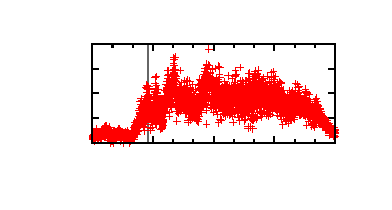
\includegraphics{/home/rik/workspace/ASL_student_project/Repositories/report-fork/Presentation/LaTeX_Template/images/windday}}%
    \gplfronttext
  \end{picture}%
\endgroup

\label{fig:wind_speed_day}}
\subfloat[][{$24\si{\hour}$ wind azimuth $[ \si{\degree} ]$ observation}]{
% GNUPLOT: LaTeX picture with Postscript
\begingroup
  \makeatletter
  \providecommand\color[2][]{%
    \GenericError{(gnuplot) \space\space\space\@spaces}{%
      Package color not loaded in conjunction with
      terminal option `colourtext'%
    }{See the gnuplot documentation for explanation.%
    }{Either use 'blacktext' in gnuplot or load the package
      color.sty in LaTeX.}%
    \renewcommand\color[2][]{}%
  }%
  \providecommand\includegraphics[2][]{%
    \GenericError{(gnuplot) \space\space\space\@spaces}{%
      Package graphicx or graphics not loaded%
    }{See the gnuplot documentation for explanation.%
    }{The gnuplot epslatex terminal needs graphicx.sty or graphics.sty.}%
    \renewcommand\includegraphics[2][]{}%
  }%
  \providecommand\rotatebox[2]{#2}%
  \@ifundefined{ifGPcolor}{%
    \newif\ifGPcolor
    \GPcolortrue
  }{}%
  \@ifundefined{ifGPblacktext}{%
    \newif\ifGPblacktext
    \GPblacktextfalse
  }{}%
  % define a \g@addto@macro without @ in the name:
  \let\gplgaddtomacro\g@addto@macro
  % define empty templates for all commands taking text:
  \gdef\gplbacktext{}%
  \gdef\gplfronttext{}%
  \makeatother
  \ifGPblacktext
    % no textcolor at all
    \def\colorrgb#1{}%
    \def\colorgray#1{}%
  \else
    % gray or color?
    \ifGPcolor
      \def\colorrgb#1{\color[rgb]{#1}}%
      \def\colorgray#1{\color[gray]{#1}}%
      \expandafter\def\csname LTw\endcsname{\color{white}}%
      \expandafter\def\csname LTb\endcsname{\color{black}}%
      \expandafter\def\csname LTa\endcsname{\color{black}}%
      \expandafter\def\csname LT0\endcsname{\color[rgb]{1,0,0}}%
      \expandafter\def\csname LT1\endcsname{\color[rgb]{0,1,0}}%
      \expandafter\def\csname LT2\endcsname{\color[rgb]{0,0,1}}%
      \expandafter\def\csname LT3\endcsname{\color[rgb]{1,0,1}}%
      \expandafter\def\csname LT4\endcsname{\color[rgb]{0,1,1}}%
      \expandafter\def\csname LT5\endcsname{\color[rgb]{1,1,0}}%
      \expandafter\def\csname LT6\endcsname{\color[rgb]{0,0,0}}%
      \expandafter\def\csname LT7\endcsname{\color[rgb]{1,0.3,0}}%
      \expandafter\def\csname LT8\endcsname{\color[rgb]{0.5,0.5,0.5}}%
    \else
      % gray
      \def\colorrgb#1{\color{black}}%
      \def\colorgray#1{\color[gray]{#1}}%
      \expandafter\def\csname LTw\endcsname{\color{white}}%
      \expandafter\def\csname LTb\endcsname{\color{black}}%
      \expandafter\def\csname LTa\endcsname{\color{black}}%
      \expandafter\def\csname LT0\endcsname{\color{black}}%
      \expandafter\def\csname LT1\endcsname{\color{black}}%
      \expandafter\def\csname LT2\endcsname{\color{black}}%
      \expandafter\def\csname LT3\endcsname{\color{black}}%
      \expandafter\def\csname LT4\endcsname{\color{black}}%
      \expandafter\def\csname LT5\endcsname{\color{black}}%
      \expandafter\def\csname LT6\endcsname{\color{black}}%
      \expandafter\def\csname LT7\endcsname{\color{black}}%
      \expandafter\def\csname LT8\endcsname{\color{black}}%
    \fi
  \fi
  \setlength{\unitlength}{0.0500bp}%
  \begin{picture}(3454.00,2266.00)%
    \gplgaddtomacro\gplbacktext{%
      \csname LTb\endcsname%
      \put(726,704){\makebox(0,0)[r]{\strut{} 0}}%
      \put(726,1028){\makebox(0,0)[r]{\strut{} 90}}%
      \put(726,1353){\makebox(0,0)[r]{\strut{} 180}}%
      \put(726,1677){\makebox(0,0)[r]{\strut{} 270}}%
      \put(726,2001){\makebox(0,0)[r]{\strut{} 360}}%
      \put(858,484){\makebox(0,0){\strut{}00}}%
      \put(1408,484){\makebox(0,0){\strut{}06}}%
      \put(1958,484){\makebox(0,0){\strut{}12}}%
      \put(2507,484){\makebox(0,0){\strut{}18}}%
      \put(3057,484){\makebox(0,0){\strut{}00}}%
      \put(1957,154){\makebox(0,0){\strut{}time $[\si{\hour}]$}}%
    }%
    \gplgaddtomacro\gplfronttext{%
    }%
    \gplbacktext
    \put(0,0){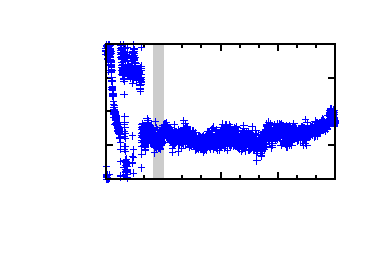
\includegraphics{/home/rik/workspace/ASL_student_project/Repositories/report-fork/Report/images/windaziday}}%
    \gplfronttext
  \end{picture}%
\endgroup

\label{fig:wind_azi_day}}
\qquad
\subfloat[][{Wind speeds $[ \si{\metre\per\second} ]$ from \formattime{5}{0}{0} to \formattime{6}{0}{0} }]{
% GNUPLOT: LaTeX picture with Postscript
\begingroup
  \makeatletter
  \providecommand\color[2][]{%
    \GenericError{(gnuplot) \space\space\space\@spaces}{%
      Package color not loaded in conjunction with
      terminal option `colourtext'%
    }{See the gnuplot documentation for explanation.%
    }{Either use 'blacktext' in gnuplot or load the package
      color.sty in LaTeX.}%
    \renewcommand\color[2][]{}%
  }%
  \providecommand\includegraphics[2][]{%
    \GenericError{(gnuplot) \space\space\space\@spaces}{%
      Package graphicx or graphics not loaded%
    }{See the gnuplot documentation for explanation.%
    }{The gnuplot epslatex terminal needs graphicx.sty or graphics.sty.}%
    \renewcommand\includegraphics[2][]{}%
  }%
  \providecommand\rotatebox[2]{#2}%
  \@ifundefined{ifGPcolor}{%
    \newif\ifGPcolor
    \GPcolortrue
  }{}%
  \@ifundefined{ifGPblacktext}{%
    \newif\ifGPblacktext
    \GPblacktextfalse
  }{}%
  % define a \g@addto@macro without @ in the name:
  \let\gplgaddtomacro\g@addto@macro
  % define empty templates for all commands taking text:
  \gdef\gplbacktext{}%
  \gdef\gplfronttext{}%
  \makeatother
  \ifGPblacktext
    % no textcolor at all
    \def\colorrgb#1{}%
    \def\colorgray#1{}%
  \else
    % gray or color?
    \ifGPcolor
      \def\colorrgb#1{\color[rgb]{#1}}%
      \def\colorgray#1{\color[gray]{#1}}%
      \expandafter\def\csname LTw\endcsname{\color{white}}%
      \expandafter\def\csname LTb\endcsname{\color{black}}%
      \expandafter\def\csname LTa\endcsname{\color{black}}%
      \expandafter\def\csname LT0\endcsname{\color[rgb]{1,0,0}}%
      \expandafter\def\csname LT1\endcsname{\color[rgb]{0,1,0}}%
      \expandafter\def\csname LT2\endcsname{\color[rgb]{0,0,1}}%
      \expandafter\def\csname LT3\endcsname{\color[rgb]{1,0,1}}%
      \expandafter\def\csname LT4\endcsname{\color[rgb]{0,1,1}}%
      \expandafter\def\csname LT5\endcsname{\color[rgb]{1,1,0}}%
      \expandafter\def\csname LT6\endcsname{\color[rgb]{0,0,0}}%
      \expandafter\def\csname LT7\endcsname{\color[rgb]{1,0.3,0}}%
      \expandafter\def\csname LT8\endcsname{\color[rgb]{0.5,0.5,0.5}}%
    \else
      % gray
      \def\colorrgb#1{\color{black}}%
      \def\colorgray#1{\color[gray]{#1}}%
      \expandafter\def\csname LTw\endcsname{\color{white}}%
      \expandafter\def\csname LTb\endcsname{\color{black}}%
      \expandafter\def\csname LTa\endcsname{\color{black}}%
      \expandafter\def\csname LT0\endcsname{\color{black}}%
      \expandafter\def\csname LT1\endcsname{\color{black}}%
      \expandafter\def\csname LT2\endcsname{\color{black}}%
      \expandafter\def\csname LT3\endcsname{\color{black}}%
      \expandafter\def\csname LT4\endcsname{\color{black}}%
      \expandafter\def\csname LT5\endcsname{\color{black}}%
      \expandafter\def\csname LT6\endcsname{\color{black}}%
      \expandafter\def\csname LT7\endcsname{\color{black}}%
      \expandafter\def\csname LT8\endcsname{\color{black}}%
    \fi
  \fi
  \setlength{\unitlength}{0.0500bp}%
  \begin{picture}(3454.00,2266.00)%
    \gplgaddtomacro\gplbacktext{%
      \csname LTb\endcsname%
      \put(594,704){\makebox(0,0)[r]{\strut{} 0}}%
      \put(594,1028){\makebox(0,0)[r]{\strut{} 4}}%
      \put(594,1353){\makebox(0,0)[r]{\strut{} 8}}%
      \put(594,1677){\makebox(0,0)[r]{\strut{} 12}}%
      \put(594,2001){\makebox(0,0)[r]{\strut{} 16}}%
      \put(726,484){\makebox(0,0){\strut{}00}}%
      \put(1309,484){\makebox(0,0){\strut{}15}}%
      \put(1892,484){\makebox(0,0){\strut{}30}}%
      \put(2474,484){\makebox(0,0){\strut{}45}}%
      \put(3057,484){\makebox(0,0){\strut{}00}}%
      \put(1891,154){\makebox(0,0){\strut{}time $[\si{\minute}]$}}%
    }%
    \gplgaddtomacro\gplfronttext{%
    }%
    \gplbacktext
    \put(0,0){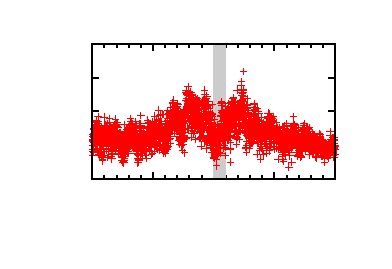
\includegraphics{/home/rik/workspace/ASL_student_project/Repositories/report-fork/Report/images/windhour}}%
    \gplfronttext
  \end{picture}%
\endgroup

\label{fig:wind_speed_hour}}
\subfloat[][{Wind azimuth $[ \si{\degree} ]$ from \formattime{5}{0}{0} to \formattime{6}{0}{0} }]{
% GNUPLOT: LaTeX picture with Postscript
\begingroup
  \makeatletter
  \providecommand\color[2][]{%
    \GenericError{(gnuplot) \space\space\space\@spaces}{%
      Package color not loaded in conjunction with
      terminal option `colourtext'%
    }{See the gnuplot documentation for explanation.%
    }{Either use 'blacktext' in gnuplot or load the package
      color.sty in LaTeX.}%
    \renewcommand\color[2][]{}%
  }%
  \providecommand\includegraphics[2][]{%
    \GenericError{(gnuplot) \space\space\space\@spaces}{%
      Package graphicx or graphics not loaded%
    }{See the gnuplot documentation for explanation.%
    }{The gnuplot epslatex terminal needs graphicx.sty or graphics.sty.}%
    \renewcommand\includegraphics[2][]{}%
  }%
  \providecommand\rotatebox[2]{#2}%
  \@ifundefined{ifGPcolor}{%
    \newif\ifGPcolor
    \GPcolortrue
  }{}%
  \@ifundefined{ifGPblacktext}{%
    \newif\ifGPblacktext
    \GPblacktextfalse
  }{}%
  % define a \g@addto@macro without @ in the name:
  \let\gplgaddtomacro\g@addto@macro
  % define empty templates for all commands taking text:
  \gdef\gplbacktext{}%
  \gdef\gplfronttext{}%
  \makeatother
  \ifGPblacktext
    % no textcolor at all
    \def\colorrgb#1{}%
    \def\colorgray#1{}%
  \else
    % gray or color?
    \ifGPcolor
      \def\colorrgb#1{\color[rgb]{#1}}%
      \def\colorgray#1{\color[gray]{#1}}%
      \expandafter\def\csname LTw\endcsname{\color{white}}%
      \expandafter\def\csname LTb\endcsname{\color{black}}%
      \expandafter\def\csname LTa\endcsname{\color{black}}%
      \expandafter\def\csname LT0\endcsname{\color[rgb]{1,0,0}}%
      \expandafter\def\csname LT1\endcsname{\color[rgb]{0,1,0}}%
      \expandafter\def\csname LT2\endcsname{\color[rgb]{0,0,1}}%
      \expandafter\def\csname LT3\endcsname{\color[rgb]{1,0,1}}%
      \expandafter\def\csname LT4\endcsname{\color[rgb]{0,1,1}}%
      \expandafter\def\csname LT5\endcsname{\color[rgb]{1,1,0}}%
      \expandafter\def\csname LT6\endcsname{\color[rgb]{0,0,0}}%
      \expandafter\def\csname LT7\endcsname{\color[rgb]{1,0.3,0}}%
      \expandafter\def\csname LT8\endcsname{\color[rgb]{0.5,0.5,0.5}}%
    \else
      % gray
      \def\colorrgb#1{\color{black}}%
      \def\colorgray#1{\color[gray]{#1}}%
      \expandafter\def\csname LTw\endcsname{\color{white}}%
      \expandafter\def\csname LTb\endcsname{\color{black}}%
      \expandafter\def\csname LTa\endcsname{\color{black}}%
      \expandafter\def\csname LT0\endcsname{\color{black}}%
      \expandafter\def\csname LT1\endcsname{\color{black}}%
      \expandafter\def\csname LT2\endcsname{\color{black}}%
      \expandafter\def\csname LT3\endcsname{\color{black}}%
      \expandafter\def\csname LT4\endcsname{\color{black}}%
      \expandafter\def\csname LT5\endcsname{\color{black}}%
      \expandafter\def\csname LT6\endcsname{\color{black}}%
      \expandafter\def\csname LT7\endcsname{\color{black}}%
      \expandafter\def\csname LT8\endcsname{\color{black}}%
    \fi
  \fi
  \setlength{\unitlength}{0.0500bp}%
  \begin{picture}(3454.00,2266.00)%
    \gplgaddtomacro\gplbacktext{%
      \csname LTb\endcsname%
      \put(726,704){\makebox(0,0)[r]{\strut{} 0}}%
      \put(726,1028){\makebox(0,0)[r]{\strut{} 45}}%
      \put(726,1353){\makebox(0,0)[r]{\strut{} 90}}%
      \put(726,1677){\makebox(0,0)[r]{\strut{} 135}}%
      \put(726,2001){\makebox(0,0)[r]{\strut{} 180}}%
      \put(858,484){\makebox(0,0){\strut{}00}}%
      \put(1408,484){\makebox(0,0){\strut{}15}}%
      \put(1958,484){\makebox(0,0){\strut{}30}}%
      \put(2507,484){\makebox(0,0){\strut{}45}}%
      \put(3057,484){\makebox(0,0){\strut{}00}}%
      \put(1957,154){\makebox(0,0){\strut{}time $[\si{\minute}]$}}%
    }%
    \gplgaddtomacro\gplfronttext{%
    }%
    \gplbacktext
    \put(0,0){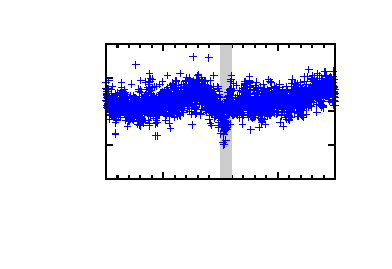
\includegraphics{/home/rik/workspace/ASL_student_project/Repositories/report-fork/Report/images/windazihour}}%
    \gplfronttext
  \end{picture}%
\endgroup

\label{fig:wind_azi_hour}}
\qquad
\subfloat[][{Wind speed $[ \si{\metre\per\second} ]$ from \formattime{5}{30}{0} to \formattime{5}{33}{0}  }]{
% GNUPLOT: LaTeX picture with Postscript
\begingroup
  \makeatletter
  \providecommand\color[2][]{%
    \GenericError{(gnuplot) \space\space\space\@spaces}{%
      Package color not loaded in conjunction with
      terminal option `colourtext'%
    }{See the gnuplot documentation for explanation.%
    }{Either use 'blacktext' in gnuplot or load the package
      color.sty in LaTeX.}%
    \renewcommand\color[2][]{}%
  }%
  \providecommand\includegraphics[2][]{%
    \GenericError{(gnuplot) \space\space\space\@spaces}{%
      Package graphicx or graphics not loaded%
    }{See the gnuplot documentation for explanation.%
    }{The gnuplot epslatex terminal needs graphicx.sty or graphics.sty.}%
    \renewcommand\includegraphics[2][]{}%
  }%
  \providecommand\rotatebox[2]{#2}%
  \@ifundefined{ifGPcolor}{%
    \newif\ifGPcolor
    \GPcolortrue
  }{}%
  \@ifundefined{ifGPblacktext}{%
    \newif\ifGPblacktext
    \GPblacktextfalse
  }{}%
  % define a \g@addto@macro without @ in the name:
  \let\gplgaddtomacro\g@addto@macro
  % define empty templates for all commands taking text:
  \gdef\gplbacktext{}%
  \gdef\gplfronttext{}%
  \makeatother
  \ifGPblacktext
    % no textcolor at all
    \def\colorrgb#1{}%
    \def\colorgray#1{}%
  \else
    % gray or color?
    \ifGPcolor
      \def\colorrgb#1{\color[rgb]{#1}}%
      \def\colorgray#1{\color[gray]{#1}}%
      \expandafter\def\csname LTw\endcsname{\color{white}}%
      \expandafter\def\csname LTb\endcsname{\color{black}}%
      \expandafter\def\csname LTa\endcsname{\color{black}}%
      \expandafter\def\csname LT0\endcsname{\color[rgb]{1,0,0}}%
      \expandafter\def\csname LT1\endcsname{\color[rgb]{0,1,0}}%
      \expandafter\def\csname LT2\endcsname{\color[rgb]{0,0,1}}%
      \expandafter\def\csname LT3\endcsname{\color[rgb]{1,0,1}}%
      \expandafter\def\csname LT4\endcsname{\color[rgb]{0,1,1}}%
      \expandafter\def\csname LT5\endcsname{\color[rgb]{1,1,0}}%
      \expandafter\def\csname LT6\endcsname{\color[rgb]{0,0,0}}%
      \expandafter\def\csname LT7\endcsname{\color[rgb]{1,0.3,0}}%
      \expandafter\def\csname LT8\endcsname{\color[rgb]{0.5,0.5,0.5}}%
    \else
      % gray
      \def\colorrgb#1{\color{black}}%
      \def\colorgray#1{\color[gray]{#1}}%
      \expandafter\def\csname LTw\endcsname{\color{white}}%
      \expandafter\def\csname LTb\endcsname{\color{black}}%
      \expandafter\def\csname LTa\endcsname{\color{black}}%
      \expandafter\def\csname LT0\endcsname{\color{black}}%
      \expandafter\def\csname LT1\endcsname{\color{black}}%
      \expandafter\def\csname LT2\endcsname{\color{black}}%
      \expandafter\def\csname LT3\endcsname{\color{black}}%
      \expandafter\def\csname LT4\endcsname{\color{black}}%
      \expandafter\def\csname LT5\endcsname{\color{black}}%
      \expandafter\def\csname LT6\endcsname{\color{black}}%
      \expandafter\def\csname LT7\endcsname{\color{black}}%
      \expandafter\def\csname LT8\endcsname{\color{black}}%
    \fi
  \fi
  \setlength{\unitlength}{0.0500bp}%
  \begin{picture}(3454.00,1700.00)%
    \gplgaddtomacro\gplbacktext{%
      \csname LTb\endcsname%
      \put(594,484){\makebox(0,0)[r]{\strut{} 0}}%
      \put(594,643){\makebox(0,0)[r]{\strut{} 2}}%
      \put(594,801){\makebox(0,0)[r]{\strut{} 4}}%
      \put(594,960){\makebox(0,0)[r]{\strut{} 6}}%
      \put(594,1118){\makebox(0,0)[r]{\strut{} 8}}%
      \put(594,1277){\makebox(0,0)[r]{\strut{} 10}}%
      \put(594,1435){\makebox(0,0)[r]{\strut{} 12}}%
      \put(726,264){\makebox(0,0){\strut{}30}}%
      \put(1503,264){\makebox(0,0){\strut{}31}}%
      \put(2280,264){\makebox(0,0){\strut{}32}}%
      \put(3057,264){\makebox(0,0){\strut{}33}}%
      \put(1891,154){\makebox(0,0){\strut{}time $[\si{\minute}]$}}%
    }%
    \gplgaddtomacro\gplfronttext{%
    }%
    \gplbacktext
    \put(0,0){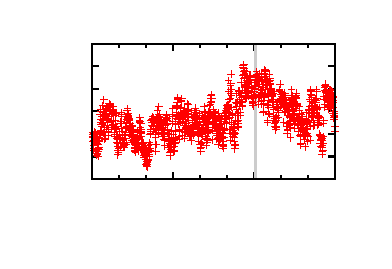
\includegraphics{/home/rik/workspace/ASL_student_project/Repositories/report-fork/Presentation/LaTeX_Template/images/windminute}}%
    \gplfronttext
  \end{picture}%
\endgroup

\label{fig:wind_speed_minutes}}
\subfloat[][{Wind azimuth $[ \si{\degree} ]$ from \formattime{5}{30}{0} to \formattime{5}{33}{0}  }]{
% GNUPLOT: LaTeX picture with Postscript
\begingroup
  \makeatletter
  \providecommand\color[2][]{%
    \GenericError{(gnuplot) \space\space\space\@spaces}{%
      Package color not loaded in conjunction with
      terminal option `colourtext'%
    }{See the gnuplot documentation for explanation.%
    }{Either use 'blacktext' in gnuplot or load the package
      color.sty in LaTeX.}%
    \renewcommand\color[2][]{}%
  }%
  \providecommand\includegraphics[2][]{%
    \GenericError{(gnuplot) \space\space\space\@spaces}{%
      Package graphicx or graphics not loaded%
    }{See the gnuplot documentation for explanation.%
    }{The gnuplot epslatex terminal needs graphicx.sty or graphics.sty.}%
    \renewcommand\includegraphics[2][]{}%
  }%
  \providecommand\rotatebox[2]{#2}%
  \@ifundefined{ifGPcolor}{%
    \newif\ifGPcolor
    \GPcolortrue
  }{}%
  \@ifundefined{ifGPblacktext}{%
    \newif\ifGPblacktext
    \GPblacktextfalse
  }{}%
  % define a \g@addto@macro without @ in the name:
  \let\gplgaddtomacro\g@addto@macro
  % define empty templates for all commands taking text:
  \gdef\gplbacktext{}%
  \gdef\gplfronttext{}%
  \makeatother
  \ifGPblacktext
    % no textcolor at all
    \def\colorrgb#1{}%
    \def\colorgray#1{}%
  \else
    % gray or color?
    \ifGPcolor
      \def\colorrgb#1{\color[rgb]{#1}}%
      \def\colorgray#1{\color[gray]{#1}}%
      \expandafter\def\csname LTw\endcsname{\color{white}}%
      \expandafter\def\csname LTb\endcsname{\color{black}}%
      \expandafter\def\csname LTa\endcsname{\color{black}}%
      \expandafter\def\csname LT0\endcsname{\color[rgb]{1,0,0}}%
      \expandafter\def\csname LT1\endcsname{\color[rgb]{0,1,0}}%
      \expandafter\def\csname LT2\endcsname{\color[rgb]{0,0,1}}%
      \expandafter\def\csname LT3\endcsname{\color[rgb]{1,0,1}}%
      \expandafter\def\csname LT4\endcsname{\color[rgb]{0,1,1}}%
      \expandafter\def\csname LT5\endcsname{\color[rgb]{1,1,0}}%
      \expandafter\def\csname LT6\endcsname{\color[rgb]{0,0,0}}%
      \expandafter\def\csname LT7\endcsname{\color[rgb]{1,0.3,0}}%
      \expandafter\def\csname LT8\endcsname{\color[rgb]{0.5,0.5,0.5}}%
    \else
      % gray
      \def\colorrgb#1{\color{black}}%
      \def\colorgray#1{\color[gray]{#1}}%
      \expandafter\def\csname LTw\endcsname{\color{white}}%
      \expandafter\def\csname LTb\endcsname{\color{black}}%
      \expandafter\def\csname LTa\endcsname{\color{black}}%
      \expandafter\def\csname LT0\endcsname{\color{black}}%
      \expandafter\def\csname LT1\endcsname{\color{black}}%
      \expandafter\def\csname LT2\endcsname{\color{black}}%
      \expandafter\def\csname LT3\endcsname{\color{black}}%
      \expandafter\def\csname LT4\endcsname{\color{black}}%
      \expandafter\def\csname LT5\endcsname{\color{black}}%
      \expandafter\def\csname LT6\endcsname{\color{black}}%
      \expandafter\def\csname LT7\endcsname{\color{black}}%
      \expandafter\def\csname LT8\endcsname{\color{black}}%
    \fi
  \fi
  \setlength{\unitlength}{0.0500bp}%
  \begin{picture}(3454.00,2266.00)%
    \gplgaddtomacro\gplbacktext{%
      \csname LTb\endcsname%
      \put(726,704){\makebox(0,0)[r]{\strut{} 0}}%
      \put(726,1028){\makebox(0,0)[r]{\strut{} 45}}%
      \put(726,1353){\makebox(0,0)[r]{\strut{} 90}}%
      \put(726,1677){\makebox(0,0)[r]{\strut{} 135}}%
      \put(726,2001){\makebox(0,0)[r]{\strut{} 180}}%
      \put(858,484){\makebox(0,0){\strut{}30}}%
      \put(1591,484){\makebox(0,0){\strut{}31}}%
      \put(2324,484){\makebox(0,0){\strut{}32}}%
      \put(3057,484){\makebox(0,0){\strut{}33}}%
      \put(1957,154){\makebox(0,0){\strut{}time $[\si{\minute}]$}}%
    }%
    \gplgaddtomacro\gplfronttext{%
    }%
    \gplbacktext
    \put(0,0){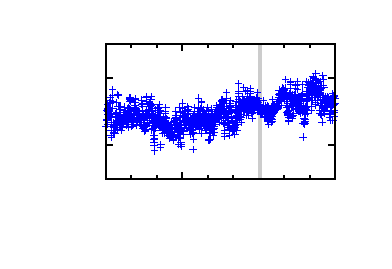
\includegraphics{/home/rik/workspace/ASL_student_project/Repositories/report-fork/Report/images/windaziminute}}%
    \gplfronttext
  \end{picture}%
\endgroup

\label{fig:wind_azi_minutes}}
\caption[Wind observations]{Wind observations. The data is gathered using an anemometer $2.76 \si{\metre}$ above ground in an open field in California, USA. More information and measurement data can be found in Google's open source data collection \cite{www:googleosb,www:googleheliostat}.}
\label{fig:wind_observations}
\end{figure}

In the bottom picture \subref{fig:wind_speed_minutes} one can detect a wind gust at \formattime{5}{32}{0}. The wind velocity suddenly reaches a peak of $10 \si{\metre\per\second}$ after averaging around $5 \si{\metre\per\second}$. 

The MAV position control action takes place in an even smaller time interval. For visualization a $3 \si{\second}$ interval has been highlighted with a vertical grey line in figure \ref{fig:wind_observations} \subref{fig:wind_speed_minutes} and \subref{fig:wind_azi_minutes}. 

Within this small time window the wind field can be modeled as a stationary stochastic process. The wind speed vector is characterised by a constant mean and variance.

\begin{align}
\E[\mathbf{w}(t)] &= \mean{\mathbf{w}} \\
\Var[\mathbf{w}(t)] &= \E\left[\left(\mathbf{w}(t)-\mean{\mathbf{w}} \right) \left(\mathbf{w}(t)-\mean{\mathbf{w}} \right)^T \right]  =\mathbf{ \Sigma }
\end{align}

Thus the differential equation governing the wind field is
\begin{align}
\d{\mathbf{w}(t)} &= \mathbf{ \Sigma } \d{\mathbf{W}(t)} \label{eq:dwind} \\
\mathbf{w}(0) &= \mean{\mathbf{w}} \label{eq:dwind_init}
\end{align}
where $\mathbf{W}(t)$ is standard Brownian motion.

A more convenient way is to state the dynamics as a discrete-time state space systems.
\begin{align}
\mathbf{w}(k+1) &= \mathbf{w}(k) + \mathbf{\discrete{\Sigma}} \boldsymbol{\varepsilon}(k) \\ 
{\varepsilon}_i (k) &\sim \mathcal{N}(0,1) & \forall i \in \{ x,y,z \}
\label{eq:wind_state_space}
\end{align}


\subsection{Wind Forces}
Wind affects the MAV dynamics in two ways. On one hand it causes pressure on the multirotor surface opposed to the wind field. We call this load area drag $\mathbf{F}_A$. On the other hand the wind field influences the total rotor drag. We name this load drag force $\mathbf{F}_D$.

Schiano and others examined the effects of area drag on a Parrot AR Drone 2.0 (quadrotor) without polystyrene casing \cite{Schiano2014,www:parrot}. This MAV is a little smaller than the AscTec Firefly but the results are qualitatively comparable. They described area drag according to Rayleigh equations.

\begin{align}
\mathbf{F}_A = \frac{1}{2} C_A \rho \norm{\mathbf{w}}_2 \mathbf{w}  \label{eq:area_drag}
\end{align}
with
\begin{align*}
C_A&: & \text{area drag coefficient} \\
\rho&: &\text{air density} \\
\mathbf{w}&: &\text{wind speed in world coordinates}.
\end{align*}

In wind tunnel experiments they measured the forces on the switched off MAV for different angles of attack. They concluded that the drag coefficient is mainly a function of heading towards the wind. The worst case (largest force) equaled to $\psi = 90 \si{\degree}$, when the processor housing is exposed with the long side and thus the largest area towards the wind. 

Following rotor blade theory, the drag force is given as in equation \ref{eq:drag_force}.
\begin{align}
\mathbf{F}_W&= \sum_{i=1}^6 \omega_i \cdot  C_D \cdot _B\mathbf{\mathbf{w}}^\perp
\end{align}

Using the worst case area drag coefficient $C_A = 0.02$ from Schianos experiments and the rotor drag coefficent $C_D = \num{6.84 e-5}$ for the Firefly, we simulate the resulting forces. Figure \ref{fig:area_vs_rotor_drag} shows the area and the rotor drag at different wind speeds and a hovering Firefly.    

\begin{figure} 
\centering 
% This file was created by matlab2tikz.
% Minimal pgfplots version: 1.3
%
%The latest updates can be retrieved from
%  http://www.mathworks.com/matlabcentral/fileexchange/22022-matlab2tikz
%where you can also make suggestions and rate matlab2tikz.
%
\definecolor{mycolor1}{rgb}{0.00000,0.44700,0.74100}%
\definecolor{mycolor2}{rgb}{0.85000,0.32500,0.09800}%
%
\begin{tikzpicture}

\begin{axis}[%
width=0.95092\figurewidth,
height=\figureheight,
at={(0\figurewidth,0\figureheight)},
scale only axis,
xmin=0,
xmax=20,
xlabel={Wind velocity $[\si{\metre\per\second}]$},
ymin=0,
ymax=6,
ytick={0, 1, 2, 3, 4, 5},
ylabel={Drag force [\si{\newton}]},
legend style={legend cell align=left,align=left,draw=white!15!black}
]
\addplot [color=mycolor1,solid]
  table[row sep=crcr]{%
0	0\\
0.02002002002002	4.90981471962453e-06\\
0.04004004004004	1.96392588784981e-05\\
0.0600600600600601	4.41883324766208e-05\\
0.0800800800800801	7.85570355139925e-05\\
0.1001001001001	0.000122745367990613\\
0.12012012012012	0.000176753329906483\\
0.14014014014014	0.000240580921261602\\
0.16016016016016	0.00031422814205597\\
0.18018018018018	0.000397694992289587\\
0.2002002002002	0.000490981471962453\\
0.22022022022022	0.000594087581074568\\
0.24024024024024	0.000707013319625932\\
0.26026026026026	0.000829758687616546\\
0.28028028028028	0.000962323685046408\\
0.3003003003003	0.00110470831191552\\
0.32032032032032	0.00125691256822388\\
0.34034034034034	0.00141893645397149\\
0.36036036036036	0.00159077996915835\\
0.38038038038038	0.00177244311378446\\
0.4004004004004	0.00196392588784981\\
0.42042042042042	0.00216522829135442\\
0.44044044044044	0.00237635032429827\\
0.46046046046046	0.00259729198668138\\
0.48048048048048	0.00282805327850373\\
0.500500500500501	0.00306863419976533\\
0.520520520520521	0.00331903475046618\\
0.540540540540541	0.00357925493060628\\
0.560560560560561	0.00384929474018563\\
0.580580580580581	0.00412915417920423\\
0.600600600600601	0.00441883324766208\\
0.620620620620621	0.00471833194555917\\
0.640640640640641	0.00502765027289552\\
0.660660660660661	0.00534678822967111\\
0.680680680680681	0.00567574581588596\\
0.700700700700701	0.00601452303154005\\
0.720720720720721	0.00636311987663339\\
0.740740740740741	0.00672153635116598\\
0.760760760760761	0.00708977245513782\\
0.780780780780781	0.00746782818854891\\
0.800800800800801	0.00785570355139925\\
0.820820820820821	0.00825339854368884\\
0.840840840840841	0.00866091316541767\\
0.860860860860861	0.00907824741658575\\
0.880880880880881	0.00950540129719309\\
0.900900900900901	0.00994237480723967\\
0.920920920920921	0.0103891679467255\\
0.940940940940941	0.0108457807156506\\
0.960960960960961	0.0113122131140149\\
0.980980980980981	0.0117884651418185\\
1.001001001001	0.0122745367990613\\
1.02102102102102	0.0127704280857434\\
1.04104104104104	0.0132761390018647\\
1.06106106106106	0.0137916695474253\\
1.08108108108108	0.0143170197224251\\
1.1011011011011	0.0148521895268642\\
1.12112112112112	0.0153971789607425\\
1.14114114114114	0.0159519880240601\\
1.16116116116116	0.0165166167168169\\
1.18118118118118	0.017091065039013\\
1.2012012012012	0.0176753329906483\\
1.22122122122122	0.0182694205717229\\
1.24124124124124	0.0188733277822367\\
1.26126126126126	0.0194870546221898\\
1.28128128128128	0.0201106010915821\\
1.3013013013013	0.0207439671904136\\
1.32132132132132	0.0213871529186845\\
1.34134134134134	0.0220401582763945\\
1.36136136136136	0.0227029832635438\\
1.38138138138138	0.0233756278801324\\
1.4014014014014	0.0240580921261602\\
1.42142142142142	0.0247503760016273\\
1.44144144144144	0.0254524795065336\\
1.46146146146146	0.0261644026408791\\
1.48148148148148	0.0268861454046639\\
1.5015015015015	0.027617707797888\\
1.52152152152152	0.0283590898205513\\
1.54154154154154	0.0291102914726538\\
1.56156156156156	0.0298713127541956\\
1.58158158158158	0.0306421536651767\\
1.6016016016016	0.031422814205597\\
1.62162162162162	0.0322132943754565\\
1.64164164164164	0.0330135941747553\\
1.66166166166166	0.0338237136034934\\
1.68168168168168	0.0346436526616707\\
1.7017017017017	0.0354734113492872\\
1.72172172172172	0.036312989666343\\
1.74174174174174	0.0371623876128381\\
1.76176176176176	0.0380216051887724\\
1.78178178178178	0.0388906423941459\\
1.8018018018018	0.0397694992289587\\
1.82182182182182	0.0406581756932107\\
1.84184184184184	0.041556671786902\\
1.86186186186186	0.0424649875100326\\
1.88188188188188	0.0433831228626023\\
1.9019019019019	0.0443110778446114\\
1.92192192192192	0.0452488524560597\\
1.94194194194194	0.0461964466969472\\
1.96196196196196	0.047153860567274\\
1.98198198198198	0.04812109406704\\
2.002002002002	0.0490981471962453\\
2.02202202202202	0.0500850199548898\\
2.04204204204204	0.0510817123429736\\
2.06206206206206	0.0520882243604966\\
2.08208208208208	0.0531045560074589\\
2.1021021021021	0.0541307072838604\\
2.12212212212212	0.0551666781897012\\
2.14214214214214	0.0562124687249812\\
2.16216216216216	0.0572680788897005\\
2.18218218218218	0.058333508683859\\
2.2022022022022	0.0594087581074568\\
2.22222222222222	0.0604938271604938\\
2.24224224224224	0.0615887158429701\\
2.26226226226226	0.0626934241548856\\
2.28228228228228	0.0638079520962404\\
2.3023023023023	0.0649322996670344\\
2.32232232232232	0.0660664668672677\\
2.34234234234234	0.0672104536969402\\
2.36236236236236	0.068364260156052\\
2.38238238238238	0.069527886244603\\
2.4024024024024	0.0707013319625932\\
2.42242242242242	0.0718845973100227\\
2.44244244244244	0.0730776822868915\\
2.46246246246246	0.0742805868931995\\
2.48248248248248	0.0754933111289468\\
2.5025025025025	0.0767158549941333\\
2.52252252252252	0.077948218488759\\
2.54254254254254	0.079190401612824\\
2.56256256256256	0.0804424043663283\\
2.58258258258258	0.0817042267492718\\
2.6026026026026	0.0829758687616546\\
2.62262262262262	0.0842573304034765\\
2.64264264264264	0.0855486116747378\\
2.66266266266266	0.0868497125754383\\
2.68268268268268	0.088160633105578\\
2.7027027027027	0.089481373265157\\
2.72272272272272	0.0908119330541753\\
2.74274274274274	0.0921523124726328\\
2.76276276276276	0.0935025115205295\\
2.78278278278278	0.0948625301978655\\
2.8028028028028	0.0962323685046408\\
2.82282282282282	0.0976120264408553\\
2.84284284284284	0.099001504006509\\
2.86286286286286	0.100400801201602\\
2.88288288288288	0.101809918026134\\
2.9029029029029	0.103228854480106\\
2.92292292292292	0.104657610563516\\
2.94294294294294	0.106096186276366\\
2.96296296296296	0.107544581618656\\
2.98298298298298	0.109002796590384\\
3.003003003003	0.110470831191552\\
3.02302302302302	0.111948685422159\\
3.04304304304304	0.113436359282205\\
3.06306306306306	0.114933852771691\\
3.08308308308308	0.116441165890615\\
3.1031031031031	0.117958298638979\\
3.12312312312312	0.119485251016783\\
3.14314314314314	0.121022023024025\\
3.16316316316316	0.122568614660707\\
3.18318318318318	0.124125025926828\\
3.2032032032032	0.125691256822388\\
3.22322322322322	0.127267307347387\\
3.24324324324324	0.128853177501826\\
3.26326326326326	0.130448867285704\\
3.28328328328328	0.132054376699021\\
3.3033033033033	0.133669705741778\\
3.32332332332332	0.135294854413974\\
3.34334334334334	0.136929822715609\\
3.36336336336336	0.138574610646683\\
3.38338338338338	0.140229218207196\\
3.4034034034034	0.141893645397149\\
3.42342342342342	0.143567892216541\\
3.44344344344344	0.145251958665372\\
3.46346346346346	0.146945844743643\\
3.48348348348348	0.148649550451352\\
3.5035035035035	0.150363075788501\\
3.52352352352352	0.152086420755089\\
3.54354354354354	0.153819585351117\\
3.56356356356356	0.155562569576584\\
3.58358358358358	0.15731537343149\\
3.6036036036036	0.159077996915835\\
3.62362362362362	0.160850440029619\\
3.64364364364364	0.162632702772843\\
3.66366366366366	0.164424785145506\\
3.68368368368368	0.166226687147608\\
3.7037037037037	0.16803840877915\\
3.72372372372372	0.16985995004013\\
3.74374374374374	0.17169131093055\\
3.76376376376376	0.173532491450409\\
3.78378378378378	0.175383491599708\\
3.8038038038038	0.177244311378446\\
3.82382382382382	0.179114950786622\\
3.84384384384384	0.180995409824239\\
3.86386386386386	0.182885688491294\\
3.88388388388388	0.184785786787789\\
3.9039039039039	0.186695704713723\\
3.92392392392392	0.188615442269096\\
3.94394394394394	0.190544999453908\\
3.96396396396396	0.19248437626816\\
3.98398398398398	0.194433572711851\\
4.004004004004	0.196392588784981\\
4.02402402402402	0.198361424487551\\
4.04404404404404	0.200340079819559\\
4.06406406406406	0.202328554781007\\
4.08408408408408	0.204326849371894\\
4.1041041041041	0.206334963592221\\
4.12412412412412	0.208352897441987\\
4.14414414414414	0.210380650921192\\
4.16416416416416	0.212418224029836\\
4.18418418418418	0.214465616767919\\
4.2042042042042	0.216522829135442\\
4.22422422422422	0.218589861132404\\
4.24424424424424	0.220666712758805\\
4.26426426426426	0.222753384014645\\
4.28428428428428	0.224849874899925\\
4.3043043043043	0.226956185414644\\
4.32432432432432	0.229072315558802\\
4.34434434434434	0.2311982653324\\
4.36436436436436	0.233334034735436\\
4.38438438438438	0.235479623767912\\
4.4044044044044	0.237635032429827\\
4.42442442442442	0.239800260721182\\
4.44444444444444	0.241975308641975\\
4.46446446446446	0.244160176192208\\
4.48448448448448	0.24635486337188\\
4.5045045045045	0.248559370180992\\
4.52452452452452	0.250773696619542\\
4.54454454454454	0.252997842687532\\
4.56456456456456	0.255231808384962\\
4.58458458458458	0.25747559371183\\
4.6046046046046	0.259729198668138\\
4.62462462462462	0.261992623253885\\
4.64464464464464	0.264265867469071\\
4.66466466466466	0.266548931313696\\
4.68468468468468	0.268841814787761\\
4.7047047047047	0.271144517891265\\
4.72472472472472	0.273457040624208\\
4.74474474474474	0.27577938298659\\
4.76476476476476	0.278111544978412\\
4.78478478478478	0.280453526599673\\
4.8048048048048	0.282805327850373\\
4.82482482482482	0.285166948730512\\
4.84484484484484	0.287538389240091\\
4.86486486486486	0.289919649379109\\
4.88488488488488	0.292310729147566\\
4.9049049049049	0.294711628545462\\
4.92492492492492	0.297122347572798\\
4.94494494494494	0.299542886229573\\
4.96496496496496	0.301973244515787\\
4.98498498498498	0.30441342243144\\
5.00500500500501	0.306863419976533\\
5.02502502502503	0.309323237151065\\
5.04504504504505	0.311792873955036\\
5.06506506506507	0.314272330388447\\
5.08508508508509	0.316761606451296\\
5.10510510510511	0.319260702143585\\
5.12512512512513	0.321769617465313\\
5.14514514514515	0.324288352416481\\
5.16516516516517	0.326816906997087\\
5.18518518518519	0.329355281207133\\
5.20520520520521	0.331903475046618\\
5.22522522522523	0.334461488515543\\
5.24524524524525	0.337029321613906\\
5.26526526526527	0.339606974341709\\
5.28528528528529	0.342194446698951\\
5.30530530530531	0.344791738685633\\
5.32532532532533	0.347398850301753\\
5.34534534534535	0.350015781547313\\
5.36536536536537	0.352642532422312\\
5.38538538538539	0.355279102926751\\
5.40540540540541	0.357925493060628\\
5.42542542542543	0.360581702823945\\
5.44544544544545	0.363247732216701\\
5.46546546546547	0.365923581238897\\
5.48548548548549	0.368609249890531\\
5.50550550550551	0.371304738171605\\
5.52552552552553	0.374010046082118\\
5.54554554554555	0.37672517362207\\
5.56556556556557	0.379450120791462\\
5.58558558558559	0.382184887590293\\
5.60560560560561	0.384929474018563\\
5.62562562562563	0.387683880076272\\
5.64564564564565	0.390448105763421\\
5.66566566566567	0.393222151080009\\
5.68568568568569	0.396006016026036\\
5.70570570570571	0.398799700601502\\
5.72572572572573	0.401603204806408\\
5.74574574574575	0.404416528640753\\
5.76576576576577	0.407239672104537\\
5.78578578578579	0.41007263519776\\
5.80580580580581	0.412915417920423\\
5.82582582582583	0.415768020272525\\
5.84584584584585	0.418630442254066\\
5.86586586586587	0.421502683865046\\
5.88588588588589	0.424384745105466\\
5.90590590590591	0.427276625975325\\
5.92592592592593	0.430178326474623\\
5.94594594594595	0.43308984660336\\
5.96596596596597	0.436011186361537\\
5.98598598598599	0.438942345749153\\
6.00600600600601	0.441883324766208\\
6.02602602602603	0.444834123412702\\
6.04604604604605	0.447794741688636\\
6.06606606606607	0.450765179594008\\
6.08608608608609	0.45374543712882\\
6.10610610610611	0.456735514293072\\
6.12612612612613	0.459735411086762\\
6.14614614614615	0.462745127509892\\
6.16616616616617	0.465764663562461\\
6.18618618618619	0.46879401924447\\
6.20620620620621	0.471833194555917\\
6.22622622622623	0.474882189496804\\
6.24624624624625	0.47794100406713\\
6.26626626626627	0.481009638266896\\
6.28628628628629	0.4840880920961\\
6.30630630630631	0.487176365554744\\
6.32632632632633	0.490274458642827\\
6.34634634634635	0.493382371360349\\
6.36636636636637	0.496500103707311\\
6.38638638638639	0.499627655683712\\
6.40640640640641	0.502765027289552\\
6.42642642642643	0.505912218524831\\
6.44644644644645	0.50906922938955\\
6.46646646646647	0.512236059883708\\
6.48648648648649	0.515412710007305\\
6.50650650650651	0.518599179760341\\
6.52652652652653	0.521795469142816\\
6.54654654654655	0.525001578154731\\
6.56656656656657	0.528217506796085\\
6.58658658658659	0.531443255066879\\
6.60660660660661	0.534678822967111\\
6.62662662662663	0.537924210496783\\
6.64664664664665	0.541179417655894\\
6.66666666666667	0.544444444444445\\
6.68668668668669	0.547719290862434\\
6.70670670670671	0.551003956909863\\
6.72672672672673	0.554298442586731\\
6.74674674674675	0.557602747893038\\
6.76676676676677	0.560916872828785\\
6.78678678678679	0.564240817393971\\
6.80680680680681	0.567574581588596\\
6.82682682682683	0.57091816541266\\
6.84684684684685	0.574271568866163\\
6.86686686686687	0.577634791949106\\
6.88688688688689	0.581007834661488\\
6.90690690690691	0.58439069700331\\
6.92692692692693	0.58778337897457\\
6.94694694694695	0.59118588057527\\
6.96696696696697	0.594598201805409\\
6.98698698698699	0.598020342664987\\
7.00700700700701	0.601452303154005\\
7.02702702702703	0.604894083272462\\
7.04704704704705	0.608345683020358\\
7.06706706706707	0.611807102397693\\
7.08708708708709	0.615278341404468\\
7.10710710710711	0.618759400040681\\
7.12712712712713	0.622250278306334\\
7.14714714714715	0.625750976201427\\
7.16716716716717	0.629261493725958\\
7.18718718718719	0.632781830879929\\
7.20720720720721	0.636311987663339\\
7.22722722722723	0.639851964076188\\
7.24724724724725	0.643401760118477\\
7.26726726726727	0.646961375790205\\
7.28728728728729	0.650530811091372\\
7.30730730730731	0.654110066021978\\
7.32732732732733	0.657699140582024\\
7.34734734734735	0.661298034771508\\
7.36736736736737	0.664906748590432\\
7.38738738738739	0.668525282038796\\
7.40740740740741	0.672153635116598\\
7.42742742742743	0.67579180782384\\
7.44744744744745	0.679439800160521\\
7.46746746746747	0.683097612126641\\
7.48748748748749	0.686765243722201\\
7.50750750750751	0.690442694947199\\
7.52752752752753	0.694129965801638\\
7.54754754754755	0.697827056285515\\
7.56756756756757	0.701533966398831\\
7.58758758758759	0.705250696141587\\
7.60760760760761	0.708977245513782\\
7.62762762762763	0.712713614515416\\
7.64764764764765	0.71645980314649\\
7.66766766766767	0.720215811407003\\
7.68768768768769	0.723981639296955\\
7.70770770770771	0.727757286816346\\
7.72772772772773	0.731542753965176\\
7.74774774774775	0.735338040743446\\
7.76776776776777	0.739143147151155\\
7.78778778778779	0.742958073188303\\
7.80780780780781	0.746782818854891\\
7.82782782782783	0.750617384150918\\
7.84784784784785	0.754461769076384\\
7.86786786786787	0.758315973631289\\
7.88788788788789	0.762179997815634\\
7.90790790790791	0.766053841629417\\
7.92792792792793	0.76993750507264\\
7.94794794794795	0.773830988145302\\
7.96796796796797	0.777734290847404\\
7.98798798798799	0.781647413178945\\
8.00800800800801	0.785570355139925\\
8.02802802802803	0.789503116730344\\
8.04804804804805	0.793445697950203\\
8.06806806806807	0.7973980987995\\
8.08808808808809	0.801360319278237\\
8.10810810810811	0.805332359386414\\
8.12812812812813	0.809314219124029\\
8.14814814814815	0.813305898491084\\
8.16816816816817	0.817307397487578\\
8.18818818818819	0.821318716113511\\
8.20820820820821	0.825339854368884\\
8.22822822822823	0.829370812253695\\
8.24824824824825	0.833411589767946\\
8.26826826826827	0.837462186911636\\
8.28828828828829	0.841522603684766\\
8.30830830830831	0.845592840087335\\
8.32832832832833	0.849672896119343\\
8.34834834834835	0.85376277178079\\
8.36836836836837	0.857862467071676\\
8.38838838838839	0.861971981992002\\
8.40840840840841	0.866091316541767\\
8.42842842842843	0.870220470720971\\
8.44844844844845	0.874359444529615\\
8.46846846846847	0.878508237967698\\
8.48848848848849	0.88266685103522\\
8.50850850850851	0.886835283732181\\
8.52852852852853	0.891013536058581\\
8.54854854854855	0.895201608014421\\
8.56856856856857	0.8993994995997\\
8.58858858858859	0.903607210814418\\
8.60860860860861	0.907824741658576\\
8.62862862862863	0.912052092132172\\
8.64864864864865	0.916289262235208\\
8.66866866866867	0.920536251967683\\
8.68868868868869	0.924793061329598\\
8.70870870870871	0.929059690320952\\
8.72872872872873	0.933336138941745\\
8.74874874874875	0.937622407191977\\
8.76876876876877	0.941918495071648\\
8.78878878878879	0.946224402580759\\
8.80880880880881	0.950540129719309\\
8.82882882882883	0.954865676487298\\
8.84884884884885	0.959201042884727\\
8.86886886886887	0.963546228911594\\
8.88888888888889	0.967901234567901\\
8.90890890890891	0.972266059853648\\
8.92892892892893	0.976640704768833\\
8.94894894894895	0.981025169313458\\
8.96896896896897	0.985419453487522\\
8.98898898898899	0.989823557291025\\
9.00900900900901	0.994237480723967\\
9.02902902902903	0.998661223786349\\
9.04904904904905	1.00309478647817\\
9.06906906906907	1.00753816879943\\
9.08908908908909	1.01199137075013\\
9.10910910910911	1.01645439233027\\
9.12912912912913	1.02092723353985\\
9.14914914914915	1.02540989437886\\
9.16916916916917	1.02990237484732\\
9.18918918918919	1.03440467494522\\
9.20920920920921	1.03891679467255\\
9.22922922922923	1.04343873402932\\
9.24924924924925	1.04797049301554\\
9.26926926926927	1.05251207163119\\
9.28928928928929	1.05706346987628\\
9.30930930930931	1.06162468775081\\
9.32932932932933	1.06619572525478\\
9.34934934934935	1.07077658238819\\
9.36936936936937	1.07536725915104\\
9.38938938938939	1.07996775554333\\
9.40940940940941	1.08457807156506\\
9.42942942942943	1.08919820721623\\
9.44944944944945	1.09382816249683\\
9.46946946946947	1.09846793740688\\
9.48948948948949	1.10311753194636\\
9.50950950950951	1.10777694611528\\
9.52952952952953	1.11244617991365\\
9.54954954954955	1.11712523334145\\
9.56956956956957	1.12181410639869\\
9.58958958958959	1.12651279908537\\
9.60960960960961	1.13122131140149\\
9.62962962962963	1.13593964334705\\
9.64964964964965	1.14066779492205\\
9.66966966966967	1.14540576612649\\
9.68968968968969	1.15015355696036\\
9.70970970970971	1.15491116742368\\
9.72972972972973	1.15967859751644\\
9.74974974974975	1.16445584723863\\
9.76976976976977	1.16924291659026\\
9.78978978978979	1.17403980557134\\
9.80980980980981	1.17884651418185\\
9.82982982982983	1.1836630424218\\
9.84984984984985	1.18848939029119\\
9.86986986986987	1.19332555779002\\
9.88988988988989	1.19817154491829\\
9.90990990990991	1.203027351676\\
9.92992992992993	1.20789297806315\\
9.94994994994995	1.21276842407974\\
9.96996996996997	1.21765368972576\\
9.98998998998999	1.22254877500123\\
10.01001001001	1.22745367990613\\
10.03003003003	1.23236840444048\\
10.0500500500501	1.23729294860426\\
10.0700700700701	1.24222731239748\\
10.0900900900901	1.24717149582014\\
10.1101101101101	1.25212549887225\\
10.1301301301301	1.25708932155379\\
10.1501501501502	1.26206296386477\\
10.1701701701702	1.26704642580518\\
10.1901901901902	1.27203970737504\\
10.2102102102102	1.27704280857434\\
10.2302302302302	1.28205572940308\\
10.2502502502503	1.28707846986125\\
10.2702702702703	1.29211102994887\\
10.2902902902903	1.29715340966592\\
10.3103103103103	1.30220560901242\\
10.3303303303303	1.30726762798835\\
10.3503503503504	1.31233946659372\\
10.3703703703704	1.31742112482853\\
10.3903903903904	1.32251260269278\\
10.4104104104104	1.32761390018647\\
10.4304304304304	1.3327250173096\\
10.4504504504505	1.33784595406217\\
10.4704704704705	1.34297671044418\\
10.4904904904905	1.34811728645562\\
10.5105105105105	1.35326768209651\\
10.5305305305305	1.35842789736684\\
10.5505505505506	1.3635979322666\\
10.5705705705706	1.3687777867958\\
10.5905905905906	1.37396746095445\\
10.6106106106106	1.37916695474253\\
10.6306306306306	1.38437626816005\\
10.6506506506507	1.38959540120701\\
10.6706706706707	1.39482435388341\\
10.6906906906907	1.40006312618925\\
10.7107107107107	1.40531171812453\\
10.7307307307307	1.41057012968925\\
10.7507507507508	1.41583836088341\\
10.7707707707708	1.421116411707\\
10.7907907907908	1.42640428216004\\
10.8108108108108	1.43170197224251\\
10.8308308308308	1.43700948195443\\
10.8508508508509	1.44232681129578\\
10.8708708708709	1.44765396026657\\
10.8908908908909	1.4529909288668\\
10.9109109109109	1.45833771709648\\
10.9309309309309	1.46369432495559\\
10.950950950951	1.46906075244414\\
10.970970970971	1.47443699956212\\
10.990990990991	1.47982306630955\\
11.011011011011	1.48521895268642\\
11.031031031031	1.49062465869273\\
11.0510510510511	1.49604018432847\\
11.0710710710711	1.50146552959366\\
11.0910910910911	1.50690069448828\\
11.1111111111111	1.51234567901235\\
11.1311311311311	1.51780048316585\\
11.1511511511512	1.52326510694879\\
11.1711711711712	1.52873955036117\\
11.1911911911912	1.53422381340299\\
11.2112112112112	1.53971789607425\\
11.2312312312312	1.54522179837495\\
11.2512512512513	1.55073552030509\\
11.2712712712713	1.55625906186467\\
11.2912912912913	1.56179242305368\\
11.3113113113113	1.56733560387214\\
11.3313313313313	1.57288860432004\\
11.3513513513514	1.57845142439737\\
11.3713713713714	1.58402406410414\\
11.3913913913914	1.58960652344036\\
11.4114114114114	1.59519880240601\\
11.4314314314314	1.6008009010011\\
11.4514514514515	1.60641281922563\\
11.4714714714715	1.6120345570796\\
11.4914914914915	1.61766611456301\\
11.5115115115115	1.62330749167586\\
11.5315315315315	1.62895868841815\\
11.5515515515516	1.63461970478987\\
11.5715715715716	1.64029054079104\\
11.5915915915916	1.64597119642165\\
11.6116116116116	1.65166167168169\\
11.6316316316316	1.65736196657118\\
11.6516516516517	1.6630720810901\\
11.6716716716717	1.66879201523846\\
11.6916916916917	1.67452176901626\\
11.7117117117117	1.6802613424235\\
11.7317317317317	1.68601073546018\\
11.7517517517518	1.6917699481263\\
11.7717717717718	1.69753898042186\\
11.7917917917918	1.70331783234686\\
11.8118118118118	1.7091065039013\\
11.8318318318318	1.71490499508518\\
11.8518518518519	1.72071330589849\\
11.8718718718719	1.72653143634125\\
11.8918918918919	1.73235938641344\\
11.9119119119119	1.73819715611507\\
11.9319319319319	1.74404474544615\\
11.951951951952	1.74990215440666\\
11.971971971972	1.75576938299661\\
11.991991991992	1.761646431216\\
12.012012012012	1.76753329906483\\
12.032032032032	1.7734299865431\\
12.0520520520521	1.77933649365081\\
12.0720720720721	1.78525282038796\\
12.0920920920921	1.79117896675454\\
12.1121121121121	1.79711493275057\\
12.1321321321321	1.80306071837603\\
12.1521521521522	1.80901632363094\\
12.1721721721722	1.81498174851528\\
12.1921921921922	1.82095699302906\\
12.2122122122122	1.82694205717229\\
12.2322322322322	1.83293694094495\\
12.2522522522523	1.83894164434705\\
12.2722722722723	1.84495616737859\\
12.2922922922923	1.85098051003957\\
12.3123123123123	1.85701467232999\\
12.3323323323323	1.86305865424985\\
12.3523523523524	1.86911245579914\\
12.3723723723724	1.87517607697788\\
12.3923923923924	1.88124951778605\\
12.4124124124124	1.88733277822367\\
12.4324324324324	1.89342585829072\\
12.4524524524525	1.89952875798722\\
12.4724724724725	1.90564147731315\\
12.4924924924925	1.91176401626852\\
12.5125125125125	1.91789637485333\\
12.5325325325325	1.92403855306758\\
12.5525525525526	1.93019055091127\\
12.5725725725726	1.9363523683844\\
12.5925925925926	1.94252400548697\\
12.6126126126126	1.94870546221898\\
12.6326326326326	1.95489673858042\\
12.6526526526527	1.96109783457131\\
12.6726726726727	1.96730875019163\\
12.6926926926927	1.9735294854414\\
12.7127127127127	1.9797600403206\\
12.7327327327327	1.98600041482924\\
12.7527527527528	1.99225060896733\\
12.7727727727728	1.99851062273485\\
12.7927927927928	2.00478045613181\\
12.8128128128128	2.01106010915821\\
12.8328328328328	2.01734958181405\\
12.8528528528529	2.02364887409933\\
12.8728728728729	2.02995798601404\\
12.8928928928929	2.0362769175582\\
12.9129129129129	2.0426056687318\\
12.9329329329329	2.04894423953483\\
12.952952952953	2.05529262996731\\
12.972972972973	2.06165084002922\\
12.992992992993	2.06801886972057\\
13.013013013013	2.07439671904136\\
13.033033033033	2.0807843879916\\
13.0530530530531	2.08718187657127\\
13.0730730730731	2.09358918478038\\
13.0930930930931	2.10000631261893\\
13.1131131131131	2.10643326008691\\
13.1331331331331	2.11287002718434\\
13.1531531531532	2.11931661391121\\
13.1731731731732	2.12577302026752\\
13.1931931931932	2.13223924625326\\
13.2132132132132	2.13871529186845\\
13.2332332332332	2.14520115711307\\
13.2532532532533	2.15169684198713\\
13.2732732732733	2.15820234649064\\
13.2932932932933	2.16471767062358\\
13.3133133133133	2.17124281438596\\
13.3333333333333	2.17777777777778\\
13.3533533533534	2.18432256079904\\
13.3733733733734	2.19087716344974\\
13.3933933933934	2.19744158572987\\
13.4134134134134	2.20401582763945\\
13.4334334334334	2.21059988917847\\
13.4534534534535	2.21719377034692\\
13.4734734734735	2.22379747114482\\
13.4934934934935	2.23041099157215\\
13.5135135135135	2.23703433162893\\
13.5335335335335	2.24366749131514\\
13.5535535535536	2.25031047063079\\
13.5735735735736	2.25696326957588\\
13.5935935935936	2.26362588815041\\
13.6136136136136	2.27029832635438\\
13.6336336336336	2.27698058418779\\
13.6536536536537	2.28367266165064\\
13.6736736736737	2.29037455874293\\
13.6936936936937	2.29708627546465\\
13.7137137137137	2.30380781181582\\
13.7337337337337	2.31053916779643\\
13.7537537537538	2.31728034340647\\
13.7737737737738	2.32403133864595\\
13.7937937937938	2.33079215351488\\
13.8138138138138	2.33756278801324\\
13.8338338338338	2.34434324214104\\
13.8538538538539	2.35113351589828\\
13.8738738738739	2.35793360928496\\
13.8938938938939	2.36474352230108\\
13.9139139139139	2.37156325494664\\
13.9339339339339	2.37839280722164\\
13.953953953954	2.38523217912607\\
13.973973973974	2.39208137065995\\
13.993993993994	2.39894038182326\\
14.014014014014	2.40580921261602\\
14.034034034034	2.41268786303821\\
14.0540540540541	2.41957633308985\\
14.0740740740741	2.42647462277092\\
14.0940940940941	2.43338273208143\\
14.1141141141141	2.44030066102138\\
14.1341341341341	2.44722840959077\\
14.1541541541542	2.4541659777896\\
14.1741741741742	2.46111336561787\\
14.1941941941942	2.46807057307558\\
14.2142142142142	2.47503760016273\\
14.2342342342342	2.48201444687931\\
14.2542542542543	2.48900111322534\\
14.2742742742743	2.4959975992008\\
14.2942942942943	2.50300390480571\\
14.3143143143143	2.51002003004005\\
14.3343343343343	2.51704597490383\\
14.3543543543544	2.52408173939705\\
14.3743743743744	2.53112732351972\\
14.3943943943944	2.53818272727182\\
14.4144144144144	2.54524795065336\\
14.4344344344344	2.55232299366434\\
14.4544544544545	2.55940785630475\\
14.4744744744745	2.56650253857461\\
14.4944944944945	2.57360704047391\\
14.5145145145145	2.58072136200264\\
14.5345345345345	2.58784550316082\\
14.5545545545546	2.59497946394843\\
14.5745745745746	2.60212324436549\\
14.5945945945946	2.60927684441198\\
14.6146146146146	2.61644026408791\\
14.6346346346346	2.62361350339328\\
14.6546546546547	2.63079656232809\\
14.6746746746747	2.63798944089234\\
14.6946946946947	2.64519213908603\\
14.7147147147147	2.65240465690916\\
14.7347347347347	2.65962699436173\\
14.7547547547548	2.66685915144374\\
14.7747747747748	2.67410112815518\\
14.7947947947948	2.68135292449607\\
14.8148148148148	2.68861454046639\\
14.8348348348348	2.69588597606616\\
14.8548548548549	2.70316723129536\\
14.8748748748749	2.710458306154\\
14.8948948948949	2.71775920064208\\
14.9149149149149	2.7250699147596\\
14.9349349349349	2.73239044850656\\
14.954954954955	2.73972080188296\\
14.974974974975	2.7470609748888\\
14.994994994995	2.75441096752408\\
15.015015015015	2.7617707797888\\
15.035035035035	2.76914041168295\\
15.0550550550551	2.77651986320655\\
15.0750750750751	2.78390913435959\\
15.0950950950951	2.79130822514206\\
15.1151151151151	2.79871713555397\\
15.1351351351351	2.80613586559533\\
15.1551551551552	2.81356441526612\\
15.1751751751752	2.82100278456635\\
15.1951951951952	2.82845097349602\\
15.2152152152152	2.83590898205513\\
15.2352352352352	2.84337681024368\\
15.2552552552553	2.85085445806167\\
15.2752752752753	2.85834192550909\\
15.2952952952953	2.86583921258596\\
15.3153153153153	2.87334631929227\\
15.3353353353353	2.88086324562801\\
15.3553553553554	2.88838999159319\\
15.3753753753754	2.89592655718782\\
15.3953953953954	2.90347294241188\\
15.4154154154154	2.91102914726538\\
15.4354354354354	2.91859517174832\\
15.4554554554555	2.92617101586071\\
15.4754754754755	2.93375667960253\\
15.4954954954955	2.94135216297378\\
15.5155155155155	2.94895746597448\\
15.5355355355355	2.95657258860462\\
15.5555555555556	2.9641975308642\\
15.5755755755756	2.97183229275321\\
15.5955955955956	2.97947687427167\\
15.6156156156156	2.98713127541956\\
15.6356356356356	2.9947954961969\\
15.6556556556557	3.00246953660367\\
15.6756756756757	3.01015339663988\\
15.6956956956957	3.01784707630553\\
15.7157157157157	3.02555057560063\\
15.7357357357357	3.03326389452516\\
15.7557557557558	3.04098703307913\\
15.7757757757758	3.04871999126253\\
15.7957957957958	3.05646276907538\\
15.8158158158158	3.06421536651767\\
15.8358358358358	3.0719777835894\\
15.8558558558559	3.07975002029056\\
15.8758758758759	3.08753207662117\\
15.8958958958959	3.09532395258121\\
15.9159159159159	3.10312564817069\\
15.9359359359359	3.11093716338962\\
15.955955955956	3.11875849823798\\
15.975975975976	3.12658965271578\\
15.995995995996	3.13443062682302\\
16.016016016016	3.1422814205597\\
16.036036036036	3.15014203392582\\
16.0560560560561	3.15801246692138\\
16.0760760760761	3.16589271954637\\
16.0960960960961	3.17378279180081\\
16.1161161161161	3.18168268368469\\
16.1361361361361	3.189592395198\\
16.1561561561562	3.19751192634076\\
16.1761761761762	3.20544127711295\\
16.1961961961962	3.21338044751458\\
16.2162162162162	3.22132943754565\\
16.2362362362362	3.22928824720617\\
16.2562562562563	3.23725687649612\\
16.2762762762763	3.24523532541551\\
16.2962962962963	3.25322359396434\\
16.3163163163163	3.2612216821426\\
16.3363363363363	3.26922958995031\\
16.3563563563564	3.27724731738746\\
16.3763763763764	3.28527486445404\\
16.3963963963964	3.29331223115007\\
16.4164164164164	3.30135941747553\\
16.4364364364364	3.30941642343044\\
16.4564564564565	3.31748324901478\\
16.4764764764765	3.32555989422856\\
16.4964964964965	3.33364635907179\\
16.5165165165165	3.34174264354445\\
16.5365365365365	3.34984874764655\\
16.5565565565566	3.35796467137809\\
16.5765765765766	3.36609041473906\\
16.5965965965966	3.37422597772948\\
16.6166166166166	3.38237136034934\\
16.6366366366366	3.39052656259864\\
16.6566566566567	3.39869158447737\\
16.6766766766767	3.40686642598555\\
16.6966966966967	3.41505108712316\\
16.7167167167167	3.42324556789021\\
16.7367367367367	3.43144986828671\\
16.7567567567568	3.43966398831264\\
16.7767767767768	3.44788792796801\\
16.7967967967968	3.45612168725282\\
16.8168168168168	3.46436526616707\\
16.8368368368368	3.47261866471076\\
16.8568568568569	3.48088188288389\\
16.8768768768769	3.48915492068645\\
16.8968968968969	3.49743777811846\\
16.9169169169169	3.50573045517991\\
16.9369369369369	3.51403295187079\\
16.956956956957	3.52234526819111\\
16.976976976977	3.53066740414088\\
16.996996996997	3.53899935972008\\
17.017017017017	3.54734113492872\\
17.037037037037	3.5556927297668\\
17.0570570570571	3.56405414423432\\
17.0770770770771	3.57242537833128\\
17.0970970970971	3.58080643205768\\
17.1171171171171	3.58919730541352\\
17.1371371371371	3.5975979983988\\
17.1571571571572	3.60600851101352\\
17.1771771771772	3.61442884325767\\
17.1971971971972	3.62285899513127\\
17.2172172172172	3.6312989666343\\
17.2372372372372	3.63974875776678\\
17.2572572572573	3.64820836852869\\
17.2772772772773	3.65667779892004\\
17.2972972972973	3.66515704894083\\
17.3173173173173	3.67364611859106\\
17.3373373373373	3.68214500787073\\
17.3573573573574	3.69065371677984\\
17.3773773773774	3.69917224531839\\
17.3973973973974	3.70770059348638\\
17.4174174174174	3.71623876128381\\
17.4374374374374	3.72478674871067\\
17.4574574574575	3.73334455576698\\
17.4774774774775	3.74191218245272\\
17.4974974974975	3.75048962876791\\
17.5175175175175	3.75907689471253\\
17.5375375375375	3.76767398028659\\
17.5575575575576	3.77628088549009\\
17.5775775775776	3.78489761032304\\
17.5975975975976	3.79352415478542\\
17.6176176176176	3.80216051887724\\
17.6376376376376	3.8108067025985\\
17.6576576576577	3.81946270594919\\
17.6776776776777	3.82812852892933\\
17.6976976976977	3.83680417153891\\
17.7177177177177	3.84548963377792\\
17.7377377377377	3.85418491564638\\
17.7577577577578	3.86289001714427\\
17.7777777777778	3.87160493827161\\
17.7977977977978	3.88032967902838\\
17.8178178178178	3.88906423941459\\
17.8378378378378	3.89780861943024\\
17.8578578578579	3.90656281907533\\
17.8778778778779	3.91532683834986\\
17.8978978978979	3.92410067725383\\
17.9179179179179	3.93288433578724\\
17.9379379379379	3.94167781395009\\
17.957957957958	3.95048111174237\\
17.977977977978	3.9592942291641\\
17.997997997998	3.96811716621526\\
18.018018018018	3.97694992289587\\
18.038038038038	3.98579249920591\\
18.0580580580581	3.9946448951454\\
18.0780780780781	4.00350711071432\\
18.0980980980981	4.01237914591268\\
18.1181181181181	4.02126100074048\\
18.1381381381381	4.03015267519772\\
18.1581581581582	4.0390541692844\\
18.1781781781782	4.04796548300052\\
18.1981981981982	4.05688661634608\\
18.2182182182182	4.06581756932107\\
18.2382382382382	4.07475834192551\\
18.2582582582583	4.08370893415939\\
18.2782782782783	4.0926693460227\\
18.2982982982983	4.10163957751545\\
18.3183183183183	4.11061962863765\\
18.3383383383383	4.11960949938928\\
18.3583583583584	4.12860918977035\\
18.3783783783784	4.13761869978086\\
18.3983983983984	4.14663802942081\\
18.4184184184184	4.1556671786902\\
18.4384384384384	4.16470614758903\\
18.4584584584585	4.1737549361173\\
18.4784784784785	4.18281354427501\\
18.4984984984985	4.19188197206215\\
18.5185185185185	4.20096021947874\\
18.5385385385385	4.21004828652476\\
18.5585585585586	4.21914617320023\\
18.5785785785786	4.22825387950513\\
18.5985985985986	4.23737140543947\\
18.6186186186186	4.24649875100326\\
18.6386386386386	4.25563591619648\\
18.6586586586587	4.26478290101914\\
18.6786786786787	4.27393970547124\\
18.6986986986987	4.28310632955278\\
18.7187187187187	4.29228277326375\\
18.7387387387387	4.30146903660417\\
18.7587587587588	4.31066511957403\\
18.7787787787788	4.31987102217332\\
18.7987987987988	4.32908674440206\\
18.8188188188188	4.33831228626023\\
18.8388388388388	4.34754764774785\\
18.8588588588589	4.3567928288649\\
18.8788788788789	4.36604782961139\\
18.8988988988989	4.37531264998733\\
18.9189189189189	4.3845872899927\\
18.9389389389389	4.39387174962751\\
18.958958958959	4.40316602889176\\
18.978978978979	4.41247012778544\\
18.998998998999	4.42178404630857\\
19.019019019019	4.43110778446114\\
19.039039039039	4.44044134224314\\
19.0590590590591	4.44978471965459\\
19.0790790790791	4.45913791669547\\
19.0990990990991	4.4685009333658\\
19.1191191191191	4.47787376966556\\
19.1391391391391	4.48725642559476\\
19.1591591591592	4.49664890115341\\
19.1791791791792	4.50605119634149\\
19.1991991991992	4.51546331115901\\
19.2192192192192	4.52488524560597\\
19.2392392392392	4.53431699968236\\
19.2592592592593	4.5437585733882\\
19.2792792792793	4.55320996672348\\
19.2992992992993	4.5626711796882\\
19.3193193193193	4.57214221228235\\
19.3393393393393	4.58162306450595\\
19.3593593593594	4.59111373635898\\
19.3793793793794	4.60061422784146\\
19.3993993993994	4.61012453895337\\
19.4194194194194	4.61964466969472\\
19.4394394394394	4.62917462006551\\
19.4594594594595	4.63871439006574\\
19.4794794794795	4.64826397969541\\
19.4994994994995	4.65782338895452\\
19.5195195195195	4.66739261784307\\
19.5395395395395	4.67697166636106\\
19.5595595595596	4.68656053450848\\
19.5795795795796	4.69615922228535\\
19.5995995995996	4.70576772969165\\
19.6196196196196	4.7153860567274\\
19.6396396396396	4.72501420339258\\
19.6596596596597	4.73465216968721\\
19.6796796796797	4.74429995561127\\
19.6996996996997	4.75395756116477\\
19.7197197197197	4.76362498634771\\
19.7397397397397	4.77330223116009\\
19.7597597597598	4.78298929560191\\
19.7797797797798	4.79268617967317\\
19.7997997997998	4.80239288337386\\
19.8198198198198	4.812109406704\\
19.8398398398398	4.82183574966358\\
19.8598598598599	4.83157191225259\\
19.8798798798799	4.84131789447105\\
19.8998998998999	4.85107369631894\\
19.9199199199199	4.86083931779627\\
19.9399399399399	4.87061475890305\\
19.95995995996	4.88040001963926\\
19.97997997998	4.89019510000491\\
20	4.9\\
};
\addlegendentry{Area};

\addplot [color=mycolor2,solid]
  table[row sep=crcr]{%
0	0\\
0.02002002002002	0.00565059566304096\\
0.04004004004004	0.0113011913260819\\
0.0600600600600601	0.0169517869891229\\
0.0800800800800801	0.0226023826521638\\
0.1001001001001	0.0282529783152048\\
0.12012012012012	0.0339035739782458\\
0.14014014014014	0.0395541696412867\\
0.16016016016016	0.0452047653043277\\
0.18018018018018	0.0508553609673686\\
0.2002002002002	0.0565059566304096\\
0.22022022022022	0.0621565522934505\\
0.24024024024024	0.0678071479564915\\
0.26026026026026	0.0734577436195325\\
0.28028028028028	0.0791083392825734\\
0.3003003003003	0.0847589349456144\\
0.32032032032032	0.0904095306086553\\
0.34034034034034	0.0960601262716963\\
0.36036036036036	0.101710721934737\\
0.38038038038038	0.107361317597778\\
0.4004004004004	0.113011913260819\\
0.42042042042042	0.11866250892386\\
0.44044044044044	0.124313104586901\\
0.46046046046046	0.129963700249942\\
0.48048048048048	0.135614295912983\\
0.500500500500501	0.141264891576024\\
0.520520520520521	0.146915487239065\\
0.540540540540541	0.152566082902106\\
0.560560560560561	0.158216678565147\\
0.580580580580581	0.163867274228188\\
0.600600600600601	0.169517869891229\\
0.620620620620621	0.17516846555427\\
0.640640640640641	0.180819061217311\\
0.660660660660661	0.186469656880352\\
0.680680680680681	0.192120252543393\\
0.700700700700701	0.197770848206434\\
0.720720720720721	0.203421443869474\\
0.740740740740741	0.209072039532515\\
0.760760760760761	0.214722635195556\\
0.780780780780781	0.220373230858597\\
0.800800800800801	0.226023826521638\\
0.820820820820821	0.231674422184679\\
0.840840840840841	0.23732501784772\\
0.860860860860861	0.242975613510761\\
0.880880880880881	0.248626209173802\\
0.900900900900901	0.254276804836843\\
0.920920920920921	0.259927400499884\\
0.940940940940941	0.265577996162925\\
0.960960960960961	0.271228591825966\\
0.980980980980981	0.276879187489007\\
1.001001001001	0.282529783152048\\
1.02102102102102	0.288180378815089\\
1.04104104104104	0.29383097447813\\
1.06106106106106	0.299481570141171\\
1.08108108108108	0.305132165804212\\
1.1011011011011	0.310782761467253\\
1.12112112112112	0.316433357130294\\
1.14114114114114	0.322083952793335\\
1.16116116116116	0.327734548456376\\
1.18118118118118	0.333385144119417\\
1.2012012012012	0.339035739782458\\
1.22122122122122	0.344686335445498\\
1.24124124124124	0.350336931108539\\
1.26126126126126	0.35598752677158\\
1.28128128128128	0.361638122434621\\
1.3013013013013	0.367288718097662\\
1.32132132132132	0.372939313760703\\
1.34134134134134	0.378589909423744\\
1.36136136136136	0.384240505086785\\
1.38138138138138	0.389891100749826\\
1.4014014014014	0.395541696412867\\
1.42142142142142	0.401192292075908\\
1.44144144144144	0.406842887738949\\
1.46146146146146	0.41249348340199\\
1.48148148148148	0.418144079065031\\
1.5015015015015	0.423794674728072\\
1.52152152152152	0.429445270391113\\
1.54154154154154	0.435095866054154\\
1.56156156156156	0.440746461717195\\
1.58158158158158	0.446397057380236\\
1.6016016016016	0.452047653043277\\
1.62162162162162	0.457698248706318\\
1.64164164164164	0.463348844369359\\
1.66166166166166	0.4689994400324\\
1.68168168168168	0.474650035695441\\
1.7017017017017	0.480300631358482\\
1.72172172172172	0.485951227021522\\
1.74174174174174	0.491601822684563\\
1.76176176176176	0.497252418347604\\
1.78178178178178	0.502903014010645\\
1.8018018018018	0.508553609673686\\
1.82182182182182	0.514204205336727\\
1.84184184184184	0.519854800999768\\
1.86186186186186	0.525505396662809\\
1.88188188188188	0.53115599232585\\
1.9019019019019	0.536806587988891\\
1.92192192192192	0.542457183651932\\
1.94194194194194	0.548107779314973\\
1.96196196196196	0.553758374978014\\
1.98198198198198	0.559408970641055\\
2.002002002002	0.565059566304096\\
2.02202202202202	0.570710161967137\\
2.04204204204204	0.576360757630178\\
2.06206206206206	0.582011353293219\\
2.08208208208208	0.58766194895626\\
2.1021021021021	0.593312544619301\\
2.12212212212212	0.598963140282342\\
2.14214214214214	0.604613735945383\\
2.16216216216216	0.610264331608424\\
2.18218218218218	0.615914927271465\\
2.2022022022022	0.621565522934506\\
2.22222222222222	0.627216118597546\\
2.24224224224224	0.632866714260587\\
2.26226226226226	0.638517309923628\\
2.28228228228228	0.644167905586669\\
2.3023023023023	0.64981850124971\\
2.32232232232232	0.655469096912751\\
2.34234234234234	0.661119692575792\\
2.36236236236236	0.666770288238833\\
2.38238238238238	0.672420883901874\\
2.4024024024024	0.678071479564915\\
2.42242242242242	0.683722075227956\\
2.44244244244244	0.689372670890997\\
2.46246246246246	0.695023266554038\\
2.48248248248248	0.700673862217079\\
2.5025025025025	0.70632445788012\\
2.52252252252252	0.711975053543161\\
2.54254254254254	0.717625649206202\\
2.56256256256256	0.723276244869243\\
2.58258258258258	0.728926840532284\\
2.6026026026026	0.734577436195325\\
2.62262262262262	0.740228031858366\\
2.64264264264264	0.745878627521407\\
2.66266266266266	0.751529223184447\\
2.68268268268268	0.757179818847488\\
2.7027027027027	0.762830414510529\\
2.72272272272272	0.76848101017357\\
2.74274274274274	0.774131605836611\\
2.76276276276276	0.779782201499652\\
2.78278278278278	0.785432797162693\\
2.8028028028028	0.791083392825734\\
2.82282282282282	0.796733988488775\\
2.84284284284284	0.802384584151816\\
2.86286286286286	0.808035179814857\\
2.88288288288288	0.813685775477898\\
2.9029029029029	0.819336371140939\\
2.92292292292292	0.82498696680398\\
2.94294294294294	0.830637562467021\\
2.96296296296296	0.836288158130062\\
2.98298298298298	0.841938753793103\\
3.003003003003	0.847589349456144\\
3.02302302302302	0.853239945119185\\
3.04304304304304	0.858890540782226\\
3.06306306306306	0.864541136445267\\
3.08308308308308	0.870191732108308\\
3.1031031031031	0.875842327771349\\
3.12312312312312	0.881492923434389\\
3.14314314314314	0.887143519097431\\
3.16316316316316	0.892794114760472\\
3.18318318318318	0.898444710423512\\
3.2032032032032	0.904095306086553\\
3.22322322322322	0.909745901749594\\
3.24324324324324	0.915396497412635\\
3.26326326326326	0.921047093075676\\
3.28328328328328	0.926697688738717\\
3.3033033033033	0.932348284401758\\
3.32332332332332	0.937998880064799\\
3.34334334334334	0.94364947572784\\
3.36336336336336	0.949300071390881\\
3.38338338338338	0.954950667053922\\
3.4034034034034	0.960601262716963\\
3.42342342342342	0.966251858380004\\
3.44344344344344	0.971902454043045\\
3.46346346346346	0.977553049706086\\
3.48348348348348	0.983203645369127\\
3.5035035035035	0.988854241032168\\
3.52352352352352	0.994504836695209\\
3.54354354354354	1.00015543235825\\
3.56356356356356	1.00580602802129\\
3.58358358358358	1.01145662368433\\
3.6036036036036	1.01710721934737\\
3.62362362362362	1.02275781501041\\
3.64364364364364	1.02840841067345\\
3.66366366366366	1.0340590063365\\
3.68368368368368	1.03970960199954\\
3.7037037037037	1.04536019766258\\
3.72372372372372	1.05101079332562\\
3.74374374374374	1.05666138898866\\
3.76376376376376	1.0623119846517\\
3.78378378378378	1.06796258031474\\
3.8038038038038	1.07361317597778\\
3.82382382382382	1.07926377164082\\
3.84384384384384	1.08491436730386\\
3.86386386386386	1.0905649629669\\
3.88388388388388	1.09621555862995\\
3.9039039039039	1.10186615429299\\
3.92392392392392	1.10751674995603\\
3.94394394394394	1.11316734561907\\
3.96396396396396	1.11881794128211\\
3.98398398398398	1.12446853694515\\
4.004004004004	1.13011913260819\\
4.02402402402402	1.13576972827123\\
4.04404404404404	1.14142032393427\\
4.06406406406406	1.14707091959731\\
4.08408408408408	1.15272151526036\\
4.1041041041041	1.1583721109234\\
4.12412412412412	1.16402270658644\\
4.14414414414414	1.16967330224948\\
4.16416416416416	1.17532389791252\\
4.18418418418418	1.18097449357556\\
4.2042042042042	1.1866250892386\\
4.22422422422422	1.19227568490164\\
4.24424424424424	1.19792628056468\\
4.26426426426426	1.20357687622772\\
4.28428428428428	1.20922747189077\\
4.3043043043043	1.21487806755381\\
4.32432432432432	1.22052866321685\\
4.34434434434434	1.22617925887989\\
4.36436436436436	1.23182985454293\\
4.38438438438438	1.23748045020597\\
4.4044044044044	1.24313104586901\\
4.42442442442442	1.24878164153205\\
4.44444444444444	1.25443223719509\\
4.46446446446446	1.26008283285813\\
4.48448448448448	1.26573342852117\\
4.5045045045045	1.27138402418422\\
4.52452452452452	1.27703461984726\\
4.54454454454454	1.2826852155103\\
4.56456456456456	1.28833581117334\\
4.58458458458458	1.29398640683638\\
4.6046046046046	1.29963700249942\\
4.62462462462462	1.30528759816246\\
4.64464464464464	1.3109381938255\\
4.66466466466466	1.31658878948854\\
4.68468468468468	1.32223938515158\\
4.7047047047047	1.32788998081463\\
4.72472472472472	1.33354057647767\\
4.74474474474474	1.33919117214071\\
4.76476476476476	1.34484176780375\\
4.78478478478478	1.35049236346679\\
4.8048048048048	1.35614295912983\\
4.82482482482482	1.36179355479287\\
4.84484484484484	1.36744415045591\\
4.86486486486486	1.37309474611895\\
4.88488488488488	1.37874534178199\\
4.9049049049049	1.38439593744503\\
4.92492492492492	1.39004653310808\\
4.94494494494494	1.39569712877112\\
4.96496496496496	1.40134772443416\\
4.98498498498498	1.4069983200972\\
5.00500500500501	1.41264891576024\\
5.02502502502503	1.41829951142328\\
5.04504504504505	1.42395010708632\\
5.06506506506507	1.42960070274936\\
5.08508508508509	1.4352512984124\\
5.10510510510511	1.44090189407544\\
5.12512512512513	1.44655248973849\\
5.14514514514515	1.45220308540153\\
5.16516516516517	1.45785368106457\\
5.18518518518519	1.46350427672761\\
5.20520520520521	1.46915487239065\\
5.22522522522523	1.47480546805369\\
5.24524524524525	1.48045606371673\\
5.26526526526527	1.48610665937977\\
5.28528528528529	1.49175725504281\\
5.30530530530531	1.49740785070585\\
5.32532532532533	1.50305844636889\\
5.34534534534535	1.50870904203194\\
5.36536536536537	1.51435963769498\\
5.38538538538539	1.52001023335802\\
5.40540540540541	1.52566082902106\\
5.42542542542543	1.5313114246841\\
5.44544544544545	1.53696202034714\\
5.46546546546547	1.54261261601018\\
5.48548548548549	1.54826321167322\\
5.50550550550551	1.55391380733626\\
5.52552552552553	1.5595644029993\\
5.54554554554555	1.56521499866235\\
5.56556556556557	1.57086559432539\\
5.58558558558559	1.57651618998843\\
5.60560560560561	1.58216678565147\\
5.62562562562563	1.58781738131451\\
5.64564564564565	1.59346797697755\\
5.66566566566567	1.59911857264059\\
5.68568568568569	1.60476916830363\\
5.70570570570571	1.61041976396667\\
5.72572572572573	1.61607035962971\\
5.74574574574575	1.62172095529276\\
5.76576576576577	1.6273715509558\\
5.78578578578579	1.63302214661884\\
5.80580580580581	1.63867274228188\\
5.82582582582583	1.64432333794492\\
5.84584584584585	1.64997393360796\\
5.86586586586587	1.655624529271\\
5.88588588588589	1.66127512493404\\
5.90590590590591	1.66692572059708\\
5.92592592592593	1.67257631626012\\
5.94594594594595	1.67822691192316\\
5.96596596596597	1.68387750758621\\
5.98598598598599	1.68952810324925\\
6.00600600600601	1.69517869891229\\
6.02602602602603	1.70082929457533\\
6.04604604604605	1.70647989023837\\
6.06606606606607	1.71213048590141\\
6.08608608608609	1.71778108156445\\
6.10610610610611	1.72343167722749\\
6.12612612612613	1.72908227289053\\
6.14614614614615	1.73473286855357\\
6.16616616616617	1.74038346421662\\
6.18618618618619	1.74603405987966\\
6.20620620620621	1.7516846555427\\
6.22622622622623	1.75733525120574\\
6.24624624624625	1.76298584686878\\
6.26626626626627	1.76863644253182\\
6.28628628628629	1.77428703819486\\
6.30630630630631	1.7799376338579\\
6.32632632632633	1.78558822952094\\
6.34634634634635	1.79123882518398\\
6.36636636636637	1.79688942084702\\
6.38638638638639	1.80254001651007\\
6.40640640640641	1.80819061217311\\
6.42642642642643	1.81384120783615\\
6.44644644644645	1.81949180349919\\
6.46646646646647	1.82514239916223\\
6.48648648648649	1.83079299482527\\
6.50650650650651	1.83644359048831\\
6.52652652652653	1.84209418615135\\
6.54654654654655	1.84774478181439\\
6.56656656656657	1.85339537747743\\
6.58658658658659	1.85904597314048\\
6.60660660660661	1.86469656880352\\
6.62662662662663	1.87034716446656\\
6.64664664664665	1.8759977601296\\
6.66666666666667	1.88164835579264\\
6.68668668668669	1.88729895145568\\
6.70670670670671	1.89294954711872\\
6.72672672672673	1.89860014278176\\
6.74674674674675	1.9042507384448\\
6.76676676676677	1.90990133410784\\
6.78678678678679	1.91555192977089\\
6.80680680680681	1.92120252543393\\
6.82682682682683	1.92685312109697\\
6.84684684684685	1.93250371676001\\
6.86686686686687	1.93815431242305\\
6.88688688688689	1.94380490808609\\
6.90690690690691	1.94945550374913\\
6.92692692692693	1.95510609941217\\
6.94694694694695	1.96075669507521\\
6.96696696696697	1.96640729073825\\
6.98698698698699	1.97205788640129\\
7.00700700700701	1.97770848206434\\
7.02702702702703	1.98335907772738\\
7.04704704704705	1.98900967339042\\
7.06706706706707	1.99466026905346\\
7.08708708708709	2.0003108647165\\
7.10710710710711	2.00596146037954\\
7.12712712712713	2.01161205604258\\
7.14714714714715	2.01726265170562\\
7.16716716716717	2.02291324736866\\
7.18718718718719	2.0285638430317\\
7.20720720720721	2.03421443869475\\
7.22722722722723	2.03986503435779\\
7.24724724724725	2.04551563002083\\
7.26726726726727	2.05116622568387\\
7.28728728728729	2.05681682134691\\
7.30730730730731	2.06246741700995\\
7.32732732732733	2.06811801267299\\
7.34734734734735	2.07376860833603\\
7.36736736736737	2.07941920399907\\
7.38738738738739	2.08506979966211\\
7.40740740740741	2.09072039532515\\
7.42742742742743	2.0963709909882\\
7.44744744744745	2.10202158665124\\
7.46746746746747	2.10767218231428\\
7.48748748748749	2.11332277797732\\
7.50750750750751	2.11897337364036\\
7.52752752752753	2.1246239693034\\
7.54754754754755	2.13027456496644\\
7.56756756756757	2.13592516062948\\
7.58758758758759	2.14157575629252\\
7.60760760760761	2.14722635195556\\
7.62762762762763	2.15287694761861\\
7.64764764764765	2.15852754328165\\
7.66766766766767	2.16417813894469\\
7.68768768768769	2.16982873460773\\
7.70770770770771	2.17547933027077\\
7.72772772772773	2.18112992593381\\
7.74774774774775	2.18678052159685\\
7.76776776776777	2.19243111725989\\
7.78778778778779	2.19808171292293\\
7.80780780780781	2.20373230858597\\
7.82782782782783	2.20938290424901\\
7.84784784784785	2.21503349991206\\
7.86786786786787	2.2206840955751\\
7.88788788788789	2.22633469123814\\
7.90790790790791	2.23198528690118\\
7.92792792792793	2.23763588256422\\
7.94794794794795	2.24328647822726\\
7.96796796796797	2.2489370738903\\
7.98798798798799	2.25458766955334\\
8.00800800800801	2.26023826521638\\
8.02802802802803	2.26588886087942\\
8.04804804804805	2.27153945654247\\
8.06806806806807	2.27719005220551\\
8.08808808808809	2.28284064786855\\
8.10810810810811	2.28849124353159\\
8.12812812812813	2.29414183919463\\
8.14814814814815	2.29979243485767\\
8.16816816816817	2.30544303052071\\
8.18818818818819	2.31109362618375\\
8.20820820820821	2.31674422184679\\
8.22822822822823	2.32239481750983\\
8.24824824824825	2.32804541317288\\
8.26826826826827	2.33369600883592\\
8.28828828828829	2.33934660449896\\
8.30830830830831	2.344997200162\\
8.32832832832833	2.35064779582504\\
8.34834834834835	2.35629839148808\\
8.36836836836837	2.36194898715112\\
8.38838838838839	2.36759958281416\\
8.40840840840841	2.3732501784772\\
8.42842842842843	2.37890077414024\\
8.44844844844845	2.38455136980328\\
8.46846846846847	2.39020196546633\\
8.48848848848849	2.39585256112937\\
8.50850850850851	2.40150315679241\\
8.52852852852853	2.40715375245545\\
8.54854854854855	2.41280434811849\\
8.56856856856857	2.41845494378153\\
8.58858858858859	2.42410553944457\\
8.60860860860861	2.42975613510761\\
8.62862862862863	2.43540673077065\\
8.64864864864865	2.44105732643369\\
8.66866866866867	2.44670792209674\\
8.68868868868869	2.45235851775978\\
8.70870870870871	2.45800911342282\\
8.72872872872873	2.46365970908586\\
8.74874874874875	2.4693103047489\\
8.76876876876877	2.47496090041194\\
8.78878878878879	2.48061149607498\\
8.80880880880881	2.48626209173802\\
8.82882882882883	2.49191268740106\\
8.84884884884885	2.4975632830641\\
8.86886886886887	2.50321387872714\\
8.88888888888889	2.50886447439019\\
8.90890890890891	2.51451507005323\\
8.92892892892893	2.52016566571627\\
8.94894894894895	2.52581626137931\\
8.96896896896897	2.53146685704235\\
8.98898898898899	2.53711745270539\\
9.00900900900901	2.54276804836843\\
9.02902902902903	2.54841864403147\\
9.04904904904905	2.55406923969451\\
9.06906906906907	2.55971983535755\\
9.08908908908909	2.5653704310206\\
9.10910910910911	2.57102102668364\\
9.12912912912913	2.57667162234668\\
9.14914914914915	2.58232221800972\\
9.16916916916917	2.58797281367276\\
9.18918918918919	2.5936234093358\\
9.20920920920921	2.59927400499884\\
9.22922922922923	2.60492460066188\\
9.24924924924925	2.61057519632492\\
9.26926926926927	2.61622579198796\\
9.28928928928929	2.621876387651\\
9.30930930930931	2.62752698331405\\
9.32932932932933	2.63317757897709\\
9.34934934934935	2.63882817464013\\
9.36936936936937	2.64447877030317\\
9.38938938938939	2.65012936596621\\
9.40940940940941	2.65577996162925\\
9.42942942942943	2.66143055729229\\
9.44944944944945	2.66708115295533\\
9.46946946946947	2.67273174861837\\
9.48948948948949	2.67838234428141\\
9.50950950950951	2.68403293994446\\
9.52952952952953	2.6896835356075\\
9.54954954954955	2.69533413127054\\
9.56956956956957	2.70098472693358\\
9.58958958958959	2.70663532259662\\
9.60960960960961	2.71228591825966\\
9.62962962962963	2.7179365139227\\
9.64964964964965	2.72358710958574\\
9.66966966966967	2.72923770524878\\
9.68968968968969	2.73488830091182\\
9.70970970970971	2.74053889657486\\
9.72972972972973	2.74618949223791\\
9.74974974974975	2.75184008790095\\
9.76976976976977	2.75749068356399\\
9.78978978978979	2.76314127922703\\
9.80980980980981	2.76879187489007\\
9.82982982982983	2.77444247055311\\
9.84984984984985	2.78009306621615\\
9.86986986986987	2.78574366187919\\
9.88988988988989	2.79139425754223\\
9.90990990990991	2.79704485320527\\
9.92992992992993	2.80269544886832\\
9.94994994994995	2.80834604453136\\
9.96996996996997	2.8139966401944\\
9.98998998998999	2.81964723585744\\
10.01001001001	2.82529783152048\\
10.03003003003	2.83094842718352\\
10.0500500500501	2.83659902284656\\
10.0700700700701	2.8422496185096\\
10.0900900900901	2.84790021417264\\
10.1101101101101	2.85355080983568\\
10.1301301301301	2.85920140549872\\
10.1501501501502	2.86485200116177\\
10.1701701701702	2.87050259682481\\
10.1901901901902	2.87615319248785\\
10.2102102102102	2.88180378815089\\
10.2302302302302	2.88745438381393\\
10.2502502502503	2.89310497947697\\
10.2702702702703	2.89875557514001\\
10.2902902902903	2.90440617080305\\
10.3103103103103	2.91005676646609\\
10.3303303303303	2.91570736212913\\
10.3503503503504	2.92135795779218\\
10.3703703703704	2.92700855345522\\
10.3903903903904	2.93265914911826\\
10.4104104104104	2.9383097447813\\
10.4304304304304	2.94396034044434\\
10.4504504504505	2.94961093610738\\
10.4704704704705	2.95526153177042\\
10.4904904904905	2.96091212743346\\
10.5105105105105	2.9665627230965\\
10.5305305305305	2.97221331875954\\
10.5505505505506	2.97786391442259\\
10.5705705705706	2.98351451008563\\
10.5905905905906	2.98916510574867\\
10.6106106106106	2.99481570141171\\
10.6306306306306	3.00046629707475\\
10.6506506506507	3.00611689273779\\
10.6706706706707	3.01176748840083\\
10.6906906906907	3.01741808406387\\
10.7107107107107	3.02306867972691\\
10.7307307307307	3.02871927538995\\
10.7507507507508	3.03436987105299\\
10.7707707707708	3.04002046671604\\
10.7907907907908	3.04567106237908\\
10.8108108108108	3.05132165804212\\
10.8308308308308	3.05697225370516\\
10.8508508508509	3.0626228493682\\
10.8708708708709	3.06827344503124\\
10.8908908908909	3.07392404069428\\
10.9109109109109	3.07957463635732\\
10.9309309309309	3.08522523202036\\
10.950950950951	3.0908758276834\\
10.970970970971	3.09652642334645\\
10.990990990991	3.10217701900949\\
11.011011011011	3.10782761467253\\
11.031031031031	3.11347821033557\\
11.0510510510511	3.11912880599861\\
11.0710710710711	3.12477940166165\\
11.0910910910911	3.13042999732469\\
11.1111111111111	3.13608059298773\\
11.1311311311311	3.14173118865077\\
11.1511511511512	3.14738178431381\\
11.1711711711712	3.15303237997685\\
11.1911911911912	3.1586829756399\\
11.2112112112112	3.16433357130294\\
11.2312312312312	3.16998416696598\\
11.2512512512513	3.17563476262902\\
11.2712712712713	3.18128535829206\\
11.2912912912913	3.1869359539551\\
11.3113113113113	3.19258654961814\\
11.3313313313313	3.19823714528118\\
11.3513513513514	3.20388774094422\\
11.3713713713714	3.20953833660726\\
11.3913913913914	3.21518893227031\\
11.4114114114114	3.22083952793335\\
11.4314314314314	3.22649012359639\\
11.4514514514515	3.23214071925943\\
11.4714714714715	3.23779131492247\\
11.4914914914915	3.24344191058551\\
11.5115115115115	3.24909250624855\\
11.5315315315315	3.25474310191159\\
11.5515515515516	3.26039369757463\\
11.5715715715716	3.26604429323767\\
11.5915915915916	3.27169488890071\\
11.6116116116116	3.27734548456376\\
11.6316316316316	3.2829960802268\\
11.6516516516517	3.28864667588984\\
11.6716716716717	3.29429727155288\\
11.6916916916917	3.29994786721592\\
11.7117117117117	3.30559846287896\\
11.7317317317317	3.311249058542\\
11.7517517517518	3.31689965420504\\
11.7717717717718	3.32255024986808\\
11.7917917917918	3.32820084553112\\
11.8118118118118	3.33385144119417\\
11.8318318318318	3.33950203685721\\
11.8518518518519	3.34515263252025\\
11.8718718718719	3.35080322818329\\
11.8918918918919	3.35645382384633\\
11.9119119119119	3.36210441950937\\
11.9319319319319	3.36775501517241\\
11.951951951952	3.37340561083545\\
11.971971971972	3.37905620649849\\
11.991991991992	3.38470680216153\\
12.012012012012	3.39035739782457\\
12.032032032032	3.39600799348762\\
12.0520520520521	3.40165858915066\\
12.0720720720721	3.4073091848137\\
12.0920920920921	3.41295978047674\\
12.1121121121121	3.41861037613978\\
12.1321321321321	3.42426097180282\\
12.1521521521522	3.42991156746586\\
12.1721721721722	3.4355621631289\\
12.1921921921922	3.44121275879194\\
12.2122122122122	3.44686335445498\\
12.2322322322322	3.45251395011803\\
12.2522522522523	3.45816454578107\\
12.2722722722723	3.46381514144411\\
12.2922922922923	3.46946573710715\\
12.3123123123123	3.47511633277019\\
12.3323323323323	3.48076692843323\\
12.3523523523524	3.48641752409627\\
12.3723723723724	3.49206811975931\\
12.3923923923924	3.49771871542235\\
12.4124124124124	3.50336931108539\\
12.4324324324324	3.50901990674844\\
12.4524524524525	3.51467050241148\\
12.4724724724725	3.52032109807452\\
12.4924924924925	3.52597169373756\\
12.5125125125125	3.5316222894006\\
12.5325325325325	3.53727288506364\\
12.5525525525526	3.54292348072668\\
12.5725725725726	3.54857407638972\\
12.5925925925926	3.55422467205276\\
12.6126126126126	3.5598752677158\\
12.6326326326326	3.56552586337885\\
12.6526526526527	3.57117645904189\\
12.6726726726727	3.57682705470493\\
12.6926926926927	3.58247765036797\\
12.7127127127127	3.58812824603101\\
12.7327327327327	3.59377884169405\\
12.7527527527528	3.59942943735709\\
12.7727727727728	3.60508003302013\\
12.7927927927928	3.61073062868317\\
12.8128128128128	3.61638122434621\\
12.8328328328328	3.62203182000925\\
12.8528528528529	3.6276824156723\\
12.8728728728729	3.63333301133534\\
12.8928928928929	3.63898360699838\\
12.9129129129129	3.64463420266142\\
12.9329329329329	3.65028479832446\\
12.952952952953	3.6559353939875\\
12.972972972973	3.66158598965054\\
12.992992992993	3.66723658531358\\
13.013013013013	3.67288718097662\\
13.033033033033	3.67853777663966\\
13.0530530530531	3.68418837230271\\
13.0730730730731	3.68983896796575\\
13.0930930930931	3.69548956362879\\
13.1131131131131	3.70114015929183\\
13.1331331331331	3.70679075495487\\
13.1531531531532	3.71244135061791\\
13.1731731731732	3.71809194628095\\
13.1931931931932	3.72374254194399\\
13.2132132132132	3.72939313760703\\
13.2332332332332	3.73504373327007\\
13.2532532532533	3.74069432893311\\
13.2732732732733	3.74634492459616\\
13.2932932932933	3.7519955202592\\
13.3133133133133	3.75764611592224\\
13.3333333333333	3.76329671158528\\
13.3533533533534	3.76894730724832\\
13.3733733733734	3.77459790291136\\
13.3933933933934	3.7802484985744\\
13.4134134134134	3.78589909423744\\
13.4334334334334	3.79154968990048\\
13.4534534534535	3.79720028556352\\
13.4734734734735	3.80285088122657\\
13.4934934934935	3.80850147688961\\
13.5135135135135	3.81415207255265\\
13.5335335335335	3.81980266821569\\
13.5535535535536	3.82545326387873\\
13.5735735735736	3.83110385954177\\
13.5935935935936	3.83675445520481\\
13.6136136136136	3.84240505086785\\
13.6336336336336	3.84805564653089\\
13.6536536536537	3.85370624219393\\
13.6736736736737	3.85935683785697\\
13.6936936936937	3.86500743352002\\
13.7137137137137	3.87065802918306\\
13.7337337337337	3.8763086248461\\
13.7537537537538	3.88195922050914\\
13.7737737737738	3.88760981617218\\
13.7937937937938	3.89326041183522\\
13.8138138138138	3.89891100749826\\
13.8338338338338	3.9045616031613\\
13.8538538538539	3.91021219882434\\
13.8738738738739	3.91586279448738\\
13.8938938938939	3.92151339015043\\
13.9139139139139	3.92716398581347\\
13.9339339339339	3.93281458147651\\
13.953953953954	3.93846517713955\\
13.973973973974	3.94411577280259\\
13.993993993994	3.94976636846563\\
14.014014014014	3.95541696412867\\
14.034034034034	3.96106755979171\\
14.0540540540541	3.96671815545475\\
14.0740740740741	3.97236875111779\\
14.0940940940941	3.97801934678083\\
14.1141141141141	3.98366994244388\\
14.1341341341341	3.98932053810692\\
14.1541541541542	3.99497113376996\\
14.1741741741742	4.000621729433\\
14.1941941941942	4.00627232509604\\
14.2142142142142	4.01192292075908\\
14.2342342342342	4.01757351642212\\
14.2542542542543	4.02322411208516\\
14.2742742742743	4.0288747077482\\
14.2942942942943	4.03452530341124\\
14.3143143143143	4.04017589907429\\
14.3343343343343	4.04582649473733\\
14.3543543543544	4.05147709040037\\
14.3743743743744	4.05712768606341\\
14.3943943943944	4.06277828172645\\
14.4144144144144	4.06842887738949\\
14.4344344344344	4.07407947305253\\
14.4544544544545	4.07973006871557\\
14.4744744744745	4.08538066437861\\
14.4944944944945	4.09103126004165\\
14.5145145145145	4.09668185570469\\
14.5345345345345	4.10233245136774\\
14.5545545545546	4.10798304703078\\
14.5745745745746	4.11363364269382\\
14.5945945945946	4.11928423835686\\
14.6146146146146	4.1249348340199\\
14.6346346346346	4.13058542968294\\
14.6546546546547	4.13623602534598\\
14.6746746746747	4.14188662100902\\
14.6946946946947	4.14753721667206\\
14.7147147147147	4.1531878123351\\
14.7347347347347	4.15883840799815\\
14.7547547547548	4.16448900366119\\
14.7747747747748	4.17013959932423\\
14.7947947947948	4.17579019498727\\
14.8148148148148	4.18144079065031\\
14.8348348348348	4.18709138631335\\
14.8548548548549	4.19274198197639\\
14.8748748748749	4.19839257763943\\
14.8948948948949	4.20404317330247\\
14.9149149149149	4.20969376896551\\
14.9349349349349	4.21534436462855\\
14.954954954955	4.2209949602916\\
14.974974974975	4.22664555595464\\
14.994994994995	4.23229615161768\\
15.015015015015	4.23794674728072\\
15.035035035035	4.24359734294376\\
15.0550550550551	4.2492479386068\\
15.0750750750751	4.25489853426984\\
15.0950950950951	4.26054912993288\\
15.1151151151151	4.26619972559592\\
15.1351351351351	4.27185032125896\\
15.1551551551552	4.27750091692201\\
15.1751751751752	4.28315151258505\\
15.1951951951952	4.28880210824809\\
15.2152152152152	4.29445270391113\\
15.2352352352352	4.30010329957417\\
15.2552552552553	4.30575389523721\\
15.2752752752753	4.31140449090025\\
15.2952952952953	4.31705508656329\\
15.3153153153153	4.32270568222633\\
15.3353353353353	4.32835627788937\\
15.3553553553554	4.33400687355242\\
15.3753753753754	4.33965746921546\\
15.3953953953954	4.3453080648785\\
15.4154154154154	4.35095866054154\\
15.4354354354354	4.35660925620458\\
15.4554554554555	4.36225985186762\\
15.4754754754755	4.36791044753066\\
15.4954954954955	4.3735610431937\\
15.5155155155155	4.37921163885674\\
15.5355355355355	4.38486223451978\\
15.5555555555556	4.39051283018282\\
15.5755755755756	4.39616342584587\\
15.5955955955956	4.40181402150891\\
15.6156156156156	4.40746461717195\\
15.6356356356356	4.41311521283499\\
15.6556556556557	4.41876580849803\\
15.6756756756757	4.42441640416107\\
15.6956956956957	4.43006699982411\\
15.7157157157157	4.43571759548715\\
15.7357357357357	4.44136819115019\\
15.7557557557558	4.44701878681323\\
15.7757757757758	4.45266938247628\\
15.7957957957958	4.45831997813932\\
15.8158158158158	4.46397057380236\\
15.8358358358358	4.4696211694654\\
15.8558558558559	4.47527176512844\\
15.8758758758759	4.48092236079148\\
15.8958958958959	4.48657295645452\\
15.9159159159159	4.49222355211756\\
15.9359359359359	4.4978741477806\\
15.955955955956	4.50352474344364\\
15.975975975976	4.50917533910668\\
15.995995995996	4.51482593476973\\
16.016016016016	4.52047653043277\\
16.036036036036	4.52612712609581\\
16.0560560560561	4.53177772175885\\
16.0760760760761	4.53742831742189\\
16.0960960960961	4.54307891308493\\
16.1161161161161	4.54872950874797\\
16.1361361361361	4.55438010441101\\
16.1561561561562	4.56003070007405\\
16.1761761761762	4.56568129573709\\
16.1961961961962	4.57133189140014\\
16.2162162162162	4.57698248706318\\
16.2362362362362	4.58263308272622\\
16.2562562562563	4.58828367838926\\
16.2762762762763	4.5939342740523\\
16.2962962962963	4.59958486971534\\
16.3163163163163	4.60523546537838\\
16.3363363363363	4.61088606104142\\
16.3563563563564	4.61653665670446\\
16.3763763763764	4.6221872523675\\
16.3963963963964	4.62783784803055\\
16.4164164164164	4.63348844369359\\
16.4364364364364	4.63913903935663\\
16.4564564564565	4.64478963501967\\
16.4764764764765	4.65044023068271\\
16.4964964964965	4.65609082634575\\
16.5165165165165	4.66174142200879\\
16.5365365365365	4.66739201767183\\
16.5565565565566	4.67304261333487\\
16.5765765765766	4.67869320899791\\
16.5965965965966	4.68434380466095\\
16.6166166166166	4.689994400324\\
16.6366366366366	4.69564499598704\\
16.6566566566567	4.70129559165008\\
16.6766766766767	4.70694618731312\\
16.6966966966967	4.71259678297616\\
16.7167167167167	4.7182473786392\\
16.7367367367367	4.72389797430224\\
16.7567567567568	4.72954856996528\\
16.7767767767768	4.73519916562832\\
16.7967967967968	4.74084976129136\\
16.8168168168168	4.74650035695441\\
16.8368368368368	4.75215095261745\\
16.8568568568569	4.75780154828049\\
16.8768768768769	4.76345214394353\\
16.8968968968969	4.76910273960657\\
16.9169169169169	4.77475333526961\\
16.9369369369369	4.78040393093265\\
16.956956956957	4.78605452659569\\
16.976976976977	4.79170512225873\\
16.996996996997	4.79735571792177\\
17.017017017017	4.80300631358481\\
17.037037037037	4.80865690924786\\
17.0570570570571	4.8143075049109\\
17.0770770770771	4.81995810057394\\
17.0970970970971	4.82560869623698\\
17.1171171171171	4.83125929190002\\
17.1371371371371	4.83690988756306\\
17.1571571571572	4.8425604832261\\
17.1771771771772	4.84821107888914\\
17.1971971971972	4.85386167455218\\
17.2172172172172	4.85951227021522\\
17.2372372372372	4.86516286587827\\
17.2572572572573	4.87081346154131\\
17.2772772772773	4.87646405720435\\
17.2972972972973	4.88211465286739\\
17.3173173173173	4.88776524853043\\
17.3373373373373	4.89341584419347\\
17.3573573573574	4.89906643985651\\
17.3773773773774	4.90471703551955\\
17.3973973973974	4.91036763118259\\
17.4174174174174	4.91601822684563\\
17.4374374374374	4.92166882250868\\
17.4574574574575	4.92731941817172\\
17.4774774774775	4.93297001383476\\
17.4974974974975	4.9386206094978\\
17.5175175175175	4.94427120516084\\
17.5375375375375	4.94992180082388\\
17.5575575575576	4.95557239648692\\
17.5775775775776	4.96122299214996\\
17.5975975975976	4.966873587813\\
17.6176176176176	4.97252418347604\\
17.6376376376376	4.97817477913908\\
17.6576576576577	4.98382537480213\\
17.6776776776777	4.98947597046517\\
17.6976976976977	4.99512656612821\\
17.7177177177177	5.00077716179125\\
17.7377377377377	5.00642775745429\\
17.7577577577578	5.01207835311733\\
17.7777777777778	5.01772894878037\\
17.7977977977978	5.02337954444341\\
17.8178178178178	5.02903014010645\\
17.8378378378378	5.03468073576949\\
17.8578578578579	5.04033133143254\\
17.8778778778779	5.04598192709558\\
17.8978978978979	5.05163252275862\\
17.9179179179179	5.05728311842166\\
17.9379379379379	5.0629337140847\\
17.957957957958	5.06858430974774\\
17.977977977978	5.07423490541078\\
17.997997997998	5.07988550107382\\
18.018018018018	5.08553609673686\\
18.038038038038	5.0911866923999\\
18.0580580580581	5.09683728806294\\
18.0780780780781	5.10248788372599\\
18.0980980980981	5.10813847938903\\
18.1181181181181	5.11378907505207\\
18.1381381381381	5.11943967071511\\
18.1581581581582	5.12509026637815\\
18.1781781781782	5.13074086204119\\
18.1981981981982	5.13639145770423\\
18.2182182182182	5.14204205336727\\
18.2382382382382	5.14769264903031\\
18.2582582582583	5.15334324469335\\
18.2782782782783	5.1589938403564\\
18.2982982982983	5.16464443601944\\
18.3183183183183	5.17029503168248\\
18.3383383383383	5.17594562734552\\
18.3583583583584	5.18159622300856\\
18.3783783783784	5.1872468186716\\
18.3983983983984	5.19289741433464\\
18.4184184184184	5.19854800999768\\
18.4384384384384	5.20419860566072\\
18.4584584584585	5.20984920132376\\
18.4784784784785	5.2154997969868\\
18.4984984984985	5.22115039264985\\
18.5185185185185	5.22680098831289\\
18.5385385385385	5.23245158397593\\
18.5585585585586	5.23810217963897\\
18.5785785785786	5.24375277530201\\
18.5985985985986	5.24940337096505\\
18.6186186186186	5.25505396662809\\
18.6386386386386	5.26070456229113\\
18.6586586586587	5.26635515795417\\
18.6786786786787	5.27200575361721\\
18.6986986986987	5.27765634928026\\
18.7187187187187	5.2833069449433\\
18.7387387387387	5.28895754060634\\
18.7587587587588	5.29460813626938\\
18.7787787787788	5.30025873193242\\
18.7987987987988	5.30590932759546\\
18.8188188188188	5.3115599232585\\
18.8388388388388	5.31721051892154\\
18.8588588588589	5.32286111458458\\
18.8788788788789	5.32851171024762\\
18.8988988988989	5.33416230591066\\
18.9189189189189	5.33981290157371\\
18.9389389389389	5.34546349723675\\
18.958958958959	5.35111409289979\\
18.978978978979	5.35676468856283\\
18.998998998999	5.36241528422587\\
19.019019019019	5.36806587988891\\
19.039039039039	5.37371647555195\\
19.0590590590591	5.37936707121499\\
19.0790790790791	5.38501766687803\\
19.0990990990991	5.39066826254107\\
19.1191191191191	5.39631885820412\\
19.1391391391391	5.40196945386716\\
19.1591591591592	5.4076200495302\\
19.1791791791792	5.41327064519324\\
19.1991991991992	5.41892124085628\\
19.2192192192192	5.42457183651932\\
19.2392392392392	5.43022243218236\\
19.2592592592593	5.4358730278454\\
19.2792792792793	5.44152362350844\\
19.2992992992993	5.44717421917148\\
19.3193193193193	5.45282481483452\\
19.3393393393393	5.45847541049757\\
19.3593593593594	5.46412600616061\\
19.3793793793794	5.46977660182365\\
19.3993993993994	5.47542719748669\\
19.4194194194194	5.48107779314973\\
19.4394394394394	5.48672838881277\\
19.4594594594595	5.49237898447581\\
19.4794794794795	5.49802958013885\\
19.4994994994995	5.50368017580189\\
19.5195195195195	5.50933077146493\\
19.5395395395395	5.51498136712798\\
19.5595595595596	5.52063196279102\\
19.5795795795796	5.52628255845406\\
19.5995995995996	5.5319331541171\\
19.6196196196196	5.53758374978014\\
19.6396396396396	5.54323434544318\\
19.6596596596597	5.54888494110622\\
19.6796796796797	5.55453553676926\\
19.6996996996997	5.5601861324323\\
19.7197197197197	5.56583672809534\\
19.7397397397397	5.57148732375839\\
19.7597597597598	5.57713791942143\\
19.7797797797798	5.58278851508447\\
19.7997997997998	5.58843911074751\\
19.8198198198198	5.59408970641055\\
19.8398398398398	5.59974030207359\\
19.8598598598599	5.60539089773663\\
19.8798798798799	5.61104149339967\\
19.8998998998999	5.61669208906271\\
19.9199199199199	5.62234268472575\\
19.9399399399399	5.62799328038879\\
19.95995995996	5.63364387605184\\
19.97997997998	5.63929447171488\\
20	5.64494506737792\\
};
\addlegendentry{Rotor};

\end{axis}
\end{tikzpicture}% 
\caption{Comparison of area and rotor drag at different wind velocities} 
\label{fig:area_vs_rotor_drag} 
\end{figure}

For small air speeds $\norm{\mathbf{w}}_2 \leq 5 \si{\metre\per\second}$ at which the MAV usually operates the rotor drag force is at least five times larger as the area drag. As a result, area drag will be neglected and only rotor drag due to wind will be modeled.

To incorporate wind explicitly into the Newton's equations \ref{eq:newton}, the air speed $\body{\boldsymbol{\nu}}$ is defined as the difference between vehicle speed $\mathbf{v}$ and wind speed $\mathbf{w}$ transformed to body coordinates.
\begin{align}
\body{\boldsymbol{\nu}} =\rotBW \left( {\mathbf{v}} - {\mathbf{w}} \right) 
\end{align}
According to the rotor drag equation \ref{eq:drag_force} and the projection \ref{eq:projection}, the total drag force in world coordinates acting on the multirotor is then
\begin{align}
\mathbf{F}_{D,total} & = \rotWB \sum_{i=1}^n \mathbf{F}_{D,i} \\ &=  - \sum_{i=1}^n \omega_i \cdot C_D \cdot \rotWB \cdot \begin{bmatrix}
1 & 0 & 0 \\
0 & 1 & 0 \\
0 & 0 & 0
\end{bmatrix}
\cdot \rotBW \left( {\mathbf{v}} - {\mathbf{w}} \right). \label{eq:total_drag}
\end{align}

%\subsubsection{Remarks on sum of rotor rates}
%The sum of rotor rates denoted in the total drag force in equation \ref{eq:total_drag} is a time varying component in our system model and should be modeled as a state.

%%%%%%%%%%%%%%%%%%%%%%%%%%%%%%%%%%%%%%%%%%%%%%%%%%%%%%%%%%%%%%%%%%%%%%%%%%%%%%%
% System Identification
%%%%%%%%%%%%%%%%%%%%%%%%%%%%%%%%%%%%%%%%%%%%%%%%%%%%%%%%%%%%%%%%%%%%%%%%%%%%%%%
\section{System Identification}
\label{sec:sys_id}
Instead of modeling the attitude controller, motor response and attitude dynamics we consider them as a black box. We approximate the attitude and thrust response of the MAV with a linear system.

\begin{equation}
\mathbf{y}(s) = \mathbf{G}(s) \mathbf{u}(s)
\end{equation}

To do this, we excite the real system with control inputs $\mathbf{u}(s)$ consisting of desired thrust $T_{ref}$, roll $\phi_{ref}$, pitch $\theta_{ref}$ and yaw $\psi_{ref}$ and measure its attained values $\mathbf{y}(s)$.

Figure \ref{pics:sys_id_model} shows a schematic model of the system. Given the control input, the attitude controller calculates a desired torque $\boldsymbol{\tau}_{ref}$. The desired motor speeds $\mathbf{n}_{ref}$ are then determined using a allocation map. These reference speeds are forwarded to the motor and the actual motor speeds affect the MAV's attitude.

\begin{figure}
\centering
\includegraphics{images/sys_id_model.tikz}
\caption{Schematic model $\mathbf{y}(s) = \mathbf{G}(s) \mathbf{u}(s)$ of black box to be identified.}
\label{pics:sys_id_model}
\end{figure}

From the experiment data the system $\mathbf{G}(s)$ is identified using MATLAB's transfer function estimation \texttt{tfest}. The method uses prediction error minimization (PEM).

The identification has to be done both for the MATLAB simulation environment and the real system.

\subsection{MATLAB Simulator}
\label{sec:matlab_simulator}
MATLAB is a good platform for prototyping control algorithms. It is easy to program and has helpful toolboxes and interfaces. We use it to simulate the non-linear inner loop dynamics depicted in figure \ref{pics:sys_id_model}.

The attitude is controlled by a geometric controller proposed by Lee \cite{Lee2010}. The allocation from desired thrust and torque to desired rotor rates is done by solving equation \ref{eq:allocation} in a least squares manner for the rotor rates. The matrix $\mathbf{A} \in \mathbb{R}^{4\times n}$ is called allocation matrix.
\begin{align}
\begin{bmatrix}
T_{ref} \\ \boldsymbol{\tau}_{ref}
\end{bmatrix} = \mathbf{A} \cdot \begin{bmatrix}
\omega_0^2 \\ \omega_1^2 \\ \vdots \\ \omega_{n-1}^2
\end{bmatrix} \label{eq:allocation} 
\end{align}
For a hexacopter with equally aligned rotors we have
\begin{align}
\mathbf{A} = \begin{bmatrix}
C_T & C_T & C_T & C_T & C_T & C_T \\
s\frac{\pi}{6} l C_T &   l C_T &  s\frac{\pi}{6} l C_T & -s\frac{\pi}{6} l C_T & -l C_T & -s\frac{\pi}{6} l C_T \\
-c\frac{\pi}{6} l C_T &  0 & c\frac{\pi}{6} l C_T &  c\frac{\pi}{6} l C_T &  0 & -c\frac{\pi}{6} l C_T \\
-C_T C_M &  C_T C_M &  -C_T C_M &   C_T C_M & -C_T C_M &  C_T C_M
\end{bmatrix}.
\end{align}
This matrix can be derived by expanding the equations of motion \ref{eq:newton} and \ref{eq:euler} and finding the corresponding thrust and torque in dependence of the squared rotor rates.

The closed loop motor dynamics are modeled as first order systems with a smaller time constant for acceleration than deceleration. Also they are limited by lower and upper bounds.
\begin{align}
\ddt \omega_i(t) =  \begin{cases}
-\frac{1}{80} \omega_i(t) + \frac{1}{80} \omega_{i,ref}(t) &\omega_{i,ref}(t) > \omega_i(t) \wedge \omega_i(t)<\omega_{max} ,\\
-\frac{1}{40} \omega_i(t) + \frac{1}{40} \omega_{i,ref}(t) &\omega_{i,ref}(t) \leq \omega_i(t)  \wedge \omega_i(t)>\omega_{min} ,\\
0  & \left( \omega_i(t)\leq \omega_{min} \wedge \omega_{i,ref}(t) \leq \omega_i(t) \right) \vee \\
& \left( \omega_i(t)\geq \omega_{max} \wedge \omega_{i,ref}(t) \geq \omega_i(t) \right).
\end{cases} \label{eq:motor_model}
\end{align}

The MAV dynamics are modeled according to the dynamics section \ref{sec:dynamics}. They include rotor drag and rolling moments.

\subsubsection{Simulated experiments}
We assume that the roll, pitch, yaw and thrust dynamics are independent from each other. The transfer function matrix $\mathbf{G}(s)$ is diagonal and we can run independent experiments for all four input/output combinations.

\begin{align}
\begin{bmatrix}
T \\ \phi \\ \theta \\ \psi
\end{bmatrix}
=
\begin{bmatrix}
G_{T_{ref} \rightarrow T} & 0 & 0 & 0 \\ 
0 & G_{\phi_{ref} \rightarrow \phi} & 0 & 0 \\ 
0 & 0 & G_{\theta_{ref} \rightarrow \theta} & 0 \\ 
0 & 0 & 0 & G_{\psi_{ref} \rightarrow \psi}  
\end{bmatrix}
\cdot
\begin{bmatrix}
T_{ref} \\ \phi_{ref} \\ \theta_{ref} \\ \psi_{ref}
\end{bmatrix}
\end{align}

Following Lennard Ljung on input design for open loop experiments \cite{ljung1999system} we generate a pseudo-random binary sequence (PRBS). This is a signal that alternates randomly between the maximum and minimum input value with a certain periodicity. It has an optimal crest factor, zero mean, and covers most frequencies. 

For all except the heading experiments, we pick a PRBS order of $n=8$, with a period length $M = 2^n-1 = 255$ which gives a sufficient resolution. $N = 10$ period repetitions are acceptable, regarding the experiment duration and coherency. For the heading experiment the PRBS order is increased to $n=12$ (period length $M=4095$) with only $N =4$ repitions, because the yaw dynamics are slower and this gives a stronger output signal.

As an example, figure \ref{fig:sys_id_phi_input} shows the roll experiment data. The amplitude levels have been chosen as
\begin{align}
T_{ref} &\in \{T_{min},T_{max}\} \\
\phi_{ref} &\in \{-22.5\si{\degree},22.5\si{\degree}\} \\
\theta_{ref} &\in \{-22.5\si{\degree},22.5\si{\degree}\} \\
\psi_{ref} &\in \{-90\si{\degree},90\si{\degree}\}
\end{align}
with
\begin{align}
T_{min} &= n \cdot \omega_{min}^2 \cdot C_T =  \num{9.2e-4} \si{\newton} , \label{eq:T_min}\\
T_{max} &= n \cdot \omega_{max}^2 \cdot C_T =  \num{36.8}\si{\newton} .\label{eq:T_max}\\
\end{align}
The first period has been dismissed to remove transients and the data detrended.

\begin{figure}
\centering
\subfloat[][{Output $\phi$}]{
% This file was created by matlab2tikz.
% Minimal pgfplots version: 1.3
%
\definecolor{mycolor1}{rgb}{0.00000,0.44700,0.74100}%
%
\begin{tikzpicture}

\begin{axis}[%
width=0.95092\figurewidth,
height=\figureheight,
at={(0\figurewidth,0\figureheight)},
scale only axis,
xmin=0,
xmax=22.94,
xlabel={time $[\si{\second}]$},
ymin=-0.174532925199433,
ymax=0.174532925199433,
ytick={-0.174532925199433,0,0.174532925199433},
yticklabels={{-10},{0},{10}},
ylabel={amplitude $[\si{\degree}]$}
]
\addplot [color=mycolor1,solid,forget plot]
  table[row sep=crcr]{%
0	0.000205986667987146\\
0.00999999999999979	-0.00386761671047415\\
0.02	-0.0080710104176326\\
0.0299999999999998	-0.0134626567634929\\
0.04	-0.0205258669417484\\
0.0499999999999998	-0.0294120329178698\\
0.0600000000000001	-0.0400942611653088\\
0.0699999999999998	-0.0524167813100445\\
0.0800000000000001	-0.0661416341633834\\
0.0899999999999999	-0.0804913862157071\\
0.1	-0.0936453269207855\\
0.11	-0.10597389765932\\
0.12	-0.11756376557217\\
0.13	-0.127207491493649\\
0.14	-0.135701345308816\\
0.15	-0.143385148457644\\
0.16	-0.148636282126839\\
0.17	-0.150784715912543\\
0.18	-0.15149685468308\\
0.19	-0.152219033223725\\
0.2	-0.153750771667385\\
0.21	-0.155893151307887\\
0.22	-0.1564771400896\\
0.23	-0.154093119684618\\
0.24	-0.14875203601525\\
0.25	-0.142558256814472\\
0.26	-0.136660008975043\\
0.27	-0.130320914522298\\
0.28	-0.124158322920631\\
0.29	-0.117556984146668\\
0.3	-0.11175040461972\\
0.31	-0.107781278800744\\
0.32	-0.105564816491061\\
0.33	-0.10301635925695\\
0.34	-0.0991598564643425\\
0.35	-0.0949448290914151\\
0.36	-0.0894226110445846\\
0.37	-0.0817873947451625\\
0.38	-0.0717588912547352\\
0.39	-0.0599056928533588\\
0.4	-0.0487215618623439\\
0.41	-0.0399818717694779\\
0.42	-0.0344722021417043\\
0.43	-0.031891576890584\\
0.44	-0.0305393786486873\\
0.45	-0.0308771891384902\\
0.46	-0.0334418780116978\\
0.47	-0.0378240055863654\\
0.48	-0.0422488651929135\\
0.49	-0.0472656965610295\\
0.5	-0.0535365855931128\\
0.51	-0.0613262303950151\\
0.52	-0.0701013728963698\\
0.53	-0.0780323296260663\\
0.54	-0.0851194269538899\\
0.55	-0.0897996119477015\\
0.56	-0.0910135508562747\\
0.57	-0.0884597494277039\\
0.58	-0.082198992463455\\
0.59	-0.0730486066369431\\
0.6	-0.0630981032827612\\
0.61	-0.0520978234040109\\
0.62	-0.0396072568631159\\
0.63	-0.0255082983676664\\
0.64	-0.0098571530357619\\
0.65	0.00716699803610889\\
0.66	0.0248095631766\\
0.67	0.0412516801319842\\
0.68	0.0563565308849991\\
0.69	0.0686888233934311\\
0.7	0.0776813566481414\\
0.71	0.0843945320835615\\
0.72	0.08798014145715\\
0.73	0.0878420317505479\\
0.74	0.0838968521606634\\
0.75	0.0763245694056694\\
0.76	0.0660327643631506\\
0.77	0.0557487204054952\\
0.78	0.0469174004145634\\
0.79	0.0382989748090647\\
0.8	0.0293695674520481\\
0.81	0.0213142612838834\\
0.82	0.0131922089962737\\
0.83	0.00409822316825622\\
0.84	-0.00578374513172029\\
0.85	-0.0142280177821977\\
0.86	-0.0197359212620368\\
0.87	-0.0222491213080456\\
0.88	-0.0232784409561561\\
0.89	-0.0228253954060763\\
0.9	-0.0225274668276127\\
0.91	-0.0236889003970361\\
0.92	-0.0263648034218833\\
0.93	-0.029081761047493\\
0.94	-0.0319937035599777\\
0.95	-0.0336232446708174\\
0.96	-0.0333960486924499\\
0.97	-0.0330569394490326\\
0.98	-0.0334403407283363\\
0.99	-0.03301234535181\\
1	-0.0311372702640228\\
1.01	-0.0289542676632256\\
1.02	-0.0261497369679724\\
1.03	-0.0235826427090914\\
1.04	-0.0207426392844455\\
1.05	-0.0183559480972406\\
1.06	-0.0158226840009608\\
1.07	-0.0138092962426287\\
1.08	-0.0111239372326222\\
1.09	-0.00731619857314447\\
1.1	-0.00361913179253852\\
1.11	0.000818023337197926\\
1.12	0.00624637522344867\\
1.13	0.0113132105517293\\
1.14	0.0168304427811316\\
1.15	0.0236093290368143\\
1.16	0.0314131616037792\\
1.17	0.0385674335219665\\
1.18	0.0451886171586387\\
1.19	0.0503480461944742\\
1.2	0.0551874013849502\\
1.21	0.0607682890727629\\
1.22	0.0676074274089608\\
1.23	0.0752964818660022\\
1.24	0.0820527240823974\\
1.25	0.0885558082962998\\
1.26	0.0950207170561217\\
1.27	0.0994990797411319\\
1.28	0.101238958404729\\
1.29	0.101408420290871\\
1.3	0.0998206722188937\\
1.31	0.0980259860951863\\
1.32	0.0973184310628115\\
1.33	0.097780921542529\\
1.34	0.0974279784439073\\
1.35	0.0948389052578643\\
1.36	0.0894222017443285\\
1.37	0.081042350054748\\
1.38	0.0703653888099343\\
1.39	0.0593876503366006\\
1.4	0.0483125064518115\\
1.41	0.038316309063122\\
1.42	0.0284371838694567\\
1.43	0.0183243606283403\\
1.44	0.00927948612366854\\
1.45	0.000962860847217256\\
1.46	-0.00528887387324662\\
1.47	-0.00902821235179014\\
1.48	-0.0115379339872197\\
1.49	-0.0126485777459483\\
1.5	-0.0133357162019863\\
1.51	-0.0126433653643597\\
1.52	-0.0102933138251398\\
1.53	-0.0081890914756256\\
1.54	-0.00777665877346742\\
1.55	-0.00972190368812538\\
1.56	-0.0142373471760638\\
1.57	-0.0212979790742248\\
1.58	-0.0301228415677172\\
1.59	-0.0380262779150322\\
1.6	-0.0431904086362455\\
1.61	-0.0448732369631735\\
1.62	-0.0429050212172186\\
1.63	-0.0374074815737111\\
1.64	-0.0286840431298055\\
1.65	-0.0177188621653573\\
1.66	-0.00732585994407198\\
1.67	0.00108001645972155\\
1.68	0.00826317290769114\\
1.69	0.0131863273245645\\
1.7	0.0155747384306242\\
1.71	0.0168051759805847\\
1.72	0.0167626050060988\\
1.73	0.0164492188154004\\
1.74	0.0154648123401739\\
1.75	0.0151695258570623\\
1.76	0.0166650978118164\\
1.77	0.0198749589432478\\
1.78	0.0232417145042144\\
1.79	0.0274198898441496\\
1.8	0.0325475044316824\\
1.81	0.0372028241496383\\
1.82	0.0416132934796915\\
1.83	0.0443641863387187\\
1.84	0.0444086991915332\\
1.85	0.0413711542960605\\
1.86	0.0357708531415443\\
1.87	0.0300364236436598\\
1.88	0.0254355726948971\\
1.89	0.0212111413257567\\
1.9	0.0179118770643041\\
1.91	0.01425428849039\\
1.92	0.00971676989490777\\
1.93	0.00603918041506913\\
1.94	0.00452258600817779\\
1.95	0.00518301652564101\\
1.96	0.00651036374666206\\
1.97	0.00913485031714801\\
1.98	0.0137085260898384\\
1.99	0.0198883509897616\\
2	0.0253756323829756\\
2.01	0.0290785894114521\\
2.02	0.0324649174465421\\
2.03	0.0362168609733087\\
2.04	0.0387134166468907\\
2.05	0.0392988495868561\\
2.06	0.0396764769217221\\
2.07	0.0412165848423853\\
2.08	0.0440282066628165\\
2.09	0.0461210354880245\\
2.1	0.0460504325713736\\
2.11	0.0437322224899084\\
2.12	0.0412028661318818\\
2.13	0.0400333805773083\\
2.14	0.0409877742867141\\
2.15	0.0437904603437281\\
2.16	0.0462023310265465\\
2.17	0.0471450975964552\\
2.18	0.0480728029396671\\
2.19	0.0502000695450013\\
2.2	0.0541031300206269\\
2.21	0.0599811443172523\\
2.22	0.0672310465373099\\
2.23	0.0733149042037093\\
2.24	0.0765438247077362\\
2.25	0.0767732833941437\\
2.26	0.0754776590729506\\
2.27	0.0721130149833151\\
2.28	0.0666827815165455\\
2.29	0.0612772140896074\\
2.3	0.0574865429675628\\
2.31	0.0560721164992533\\
2.32	0.0567536724812924\\
2.33	0.0578530572161702\\
2.34	0.0593770253814425\\
2.35	0.0603052211805999\\
2.36	0.0610971680697009\\
2.37	0.0604849147481518\\
2.38	0.0580245694511407\\
2.39	0.0555356040839683\\
2.4	0.0538956861697016\\
2.41	0.0521489510213763\\
2.42	0.0513106684282894\\
2.43	0.0517317076009718\\
2.44	0.0515769661982044\\
2.45	0.0494808622490582\\
2.46	0.0453912451241643\\
2.47	0.0413587309614869\\
2.48	0.0383917921224137\\
2.49	0.0350415407898484\\
2.5	0.0301434982276199\\
2.51	0.0237391088582944\\
2.52	0.0173728878676783\\
2.53	0.0109345532831542\\
2.54	0.00538487620942708\\
2.55	0.000222969427011451\\
2.56	-0.00385199635545294\\
2.57	-0.00805673423047823\\
2.58	-0.0134503615572729\\
2.59	-0.0205165026309321\\
2.6	-0.0294066464796499\\
2.61	-0.0400938794083914\\
2.62	-0.0524223337719323\\
2.63	-0.0661539057744492\\
2.64	-0.0805110968157107\\
2.65	-0.0936732477210235\\
2.66	-0.106010381609234\\
2.67	-0.117608948143812\\
2.68	-0.127261627001172\\
2.69	-0.135764343760269\\
2.7	-0.143456796565358\\
2.71	-0.148716868031587\\
2.72	-0.150874943003585\\
2.73	-0.151596994062468\\
2.74	-0.15232864962511\\
2.75	-0.153869034368655\\
2.76	-0.156018220942983\\
2.77	-0.156604575114142\\
2.78	-0.154218424354009\\
2.79	-0.148871578022937\\
2.8	-0.142669887603867\\
2.81	-0.136762848752457\\
2.82	-0.130414232427514\\
2.83	-0.124242049499107\\
2.84	-0.117630983523219\\
2.85	-0.111815321725985\\
2.86	-0.107838406825881\\
2.87	-0.105615447894947\\
2.88	-0.103060685245673\\
2.89	-0.0991975876699888\\
2.9	-0.0949761615141142\\
2.91	-0.0894472906224336\\
2.92	-0.0818048092358577\\
2.93	-0.0717683259583601\\
2.94	-0.0599066628098969\\
2.95	-0.048714605380599\\
2.96	-0.0399684018411668\\
2.97	-0.034454109845335\\
2.98	-0.0318706243375627\\
2.99	-0.0305164179601499\\
3	-0.0308533457692701\\
3.01	-0.0334185753942192\\
3.02	-0.0378023908717762\\
3.03	-0.0422289873870805\\
3.04	-0.0472479394216815\\
3.05	-0.0535217416119414\\
3.06	-0.0613152489349174\\
3.07	-0.0700953981529803\\
3.08	-0.0780328165222313\\
3.09	-0.0851276876061217\\
3.1	-0.089816492329367\\
3.11	-0.0910376487442647\\
3.12	-0.0884889091535898\\
3.13	-0.0822308086874335\\
3.14	-0.0730807997927422\\
3.15	-0.0631291074201956\\
3.16	-0.0521261127798495\\
3.17	-0.0396313090066959\\
3.18	-0.0255266945538803\\
3.19	-0.00986864738139706\\
3.2	0.00716341865371584\\
3.21	0.0248142776745727\\
3.22	0.0412636520933481\\
3.23	0.0563746941854812\\
3.24	0.0687110427089468\\
3.25	0.0777051063040931\\
3.26	0.0844180527900498\\
3.27	0.0880016015759745\\
3.28	0.0878598110211782\\
3.29	0.0839094459213916\\
3.3	0.0763306614451048\\
3.31	0.0660316407987835\\
3.32	0.0557413742417887\\
3.33	0.0469055548647273\\
3.34	0.0382834984929518\\
3.35	0.0293508727796403\\
3.36	0.0212933736066443\\
3.37	0.0131694802504113\\
3.38	0.00407334295331666\\
3.39	-0.00581087350686346\\
3.4	-0.0142556778134695\\
3.41	-0.0197618621670925\\
3.42	-0.0222714644112733\\
3.43	-0.0232962385939363\\
3.44	-0.0228379957183385\\
3.45	-0.0225352295755694\\
3.46	-0.0236929951499474\\
3.47	-0.0263664753287391\\
3.48	-0.0290814557426501\\
3.49	-0.0319919310159327\\
3.5	-0.0336197069307679\\
3.51	-0.0333901416570412\\
3.52	-0.0330489130713117\\
3.53	-0.0334308655393023\\
3.54	-0.0330012768116797\\
3.55	-0.0311241290468426\\
3.56	-0.0289391178869201\\
3.57	-0.0261324769136552\\
3.58	-0.0235635857511204\\
3.59	-0.0207218284598849\\
3.6	-0.0183337746350951\\
3.61	-0.0157992198851277\\
3.62	-0.0137849320290114\\
3.63	-0.0110984532152902\\
3.64	-0.00728914546764771\\
3.65	-0.00359064521721965\\
3.66	0.000848223139980623\\
3.67	0.0062786899469799\\
3.68	0.0113474064951261\\
3.69	0.0168666734382055\\
3.7	0.0236481189468032\\
3.71	0.0314549380011636\\
3.72	0.0386118984633915\\
3.73	0.0452355101505777\\
3.74	0.0503966511584856\\
3.75	0.0552375290829401\\
3.76	0.0608202235088839\\
3.77	0.067661669052961\\
3.78	0.0753531825442738\\
3.79	0.0821108414149629\\
3.8	0.0886148253147347\\
3.81	0.0950802964716236\\
3.82	0.0995579177163043\\
3.83	0.10129574172059\\
3.84	0.101462534667067\\
3.85	0.0998714632300364\\
3.86	0.0980735996902017\\
3.87	0.0973636355490071\\
3.88	0.0978245109727047\\
3.89	0.0974697885977856\\
3.9	0.0948780321193887\\
3.91	0.0894574088865139\\
3.92	0.0810723143504418\\
3.93	0.0703891756130672\\
3.94	0.0594055030572937\\
3.95	0.0483247567240838\\
3.96	0.0383239977983136\\
3.97	0.0284407097609589\\
3.98	0.0183238754458457\\
3.99	0.00927598680003558\\
4	0.000957053028693968\\
4.01	-0.0052956513288754\\
4.02	-0.00903452964705407\\
4.03	-0.011543097735036\\
4.04	-0.0126519321165883\\
4.05	-0.0133371769665933\\
4.06	-0.0126424275150624\\
4.07	-0.0102893716976726\\
4.08	-0.00818249950981961\\
4.09	-0.00776851709603939\\
4.1	-0.00971364509469892\\
4.11	-0.0142304909169093\\
4.12	-0.0212939995298008\\
4.13	-0.0301225495478883\\
4.14	-0.0380281487560848\\
4.15	-0.0431920978776802\\
4.16	-0.0448726056133364\\
4.17	-0.0429002521598007\\
4.18	-0.0373971205990646\\
4.19	-0.0286669349535553\\
4.2	-0.0176944058574682\\
4.21	-0.0072949271520915\\
4.22	0.00111583967862233\\
4.23	0.00830275453080586\\
4.24	0.0132280944206856\\
4.25	0.0156170607146735\\
4.26	0.0168471889359928\\
4.27	0.0168034556423529\\
4.28	0.0164886283805294\\
4.29	0.0155023489491082\\
4.3	0.0152054920235364\\
4.31	0.0167003633876698\\
4.32	0.0199103647372058\\
4.33	0.0232773529145989\\
4.34	0.0274561752221376\\
4.35	0.0325849124990621\\
4.36	0.037241126083012\\
4.37	0.0416523711392272\\
4.38	0.0444032075547624\\
4.39	0.0444463088648986\\
4.4	0.0414058232558869\\
4.41	0.0358013487181418\\
4.42	0.0300628157604648\\
4.43	0.0254585960810014\\
4.44	0.0212311366589801\\
4.45	0.0179294547164846\\
4.46	0.0142693802006501\\
4.47	0.00972902600664028\\
4.48	0.00604916602893028\\
4.49	0.00453149994790815\\
4.5	0.00519203253983853\\
4.51	0.0065198957760307\\
4.52	0.00914559016769346\\
4.53	0.0137214488290617\\
4.54	0.019904230242653\\
4.55	0.0253940699118174\\
4.56	0.0290986182149505\\
4.57	0.0324863143214058\\
4.58	0.0362397511996764\\
4.59	0.0387371045807338\\
4.6	0.0393223167642465\\
4.61	0.0396995852415739\\
4.62	0.0412398984253536\\
4.63	0.0440523443939129\\
4.64	0.0461456147527603\\
4.65	0.0460743434213186\\
4.66	0.0437543294373987\\
4.67	0.0412230880302165\\
4.68	0.0400524413951283\\
4.69	0.0410067693752481\\
4.7	0.0438103355243633\\
4.71	0.0462229060076086\\
4.72	0.0471656363883976\\
4.73	0.0480933071526108\\
4.74	0.0502211529784923\\
4.75	0.0541256836878007\\
4.76	0.0600061418456776\\
4.77	0.0672590810561992\\
4.78	0.0733450375208514\\
4.79	0.0765743277292255\\
4.8	0.0768024957061485\\
4.81	0.0755047390804514\\
4.82	0.0721369462151133\\
4.83	0.0667026237240167\\
4.84	0.0612931494138907\\
4.85	0.0574995858037209\\
4.86	0.0560836475453891\\
4.87	0.0567649120706476\\
4.88	0.0578643771814581\\
4.89	0.059388770029586\\
4.9	0.0603171841798545\\
4.91	0.0611093554638843\\
4.92	0.060496668602231\\
4.93	0.0580350027137794\\
4.94	0.055544757258691\\
4.95	0.0539040468305451\\
4.96	0.0521565167723151\\
4.97	0.0513179467574667\\
4.98	0.0517393701928835\\
4.99	0.0515847378756605\\
5	0.0494877696946108\\
5.01	0.045396298837701\\
5.02	0.0413619953645927\\
5.03	0.0383938528542932\\
5.04	0.0350422445910511\\
5.05	0.0301420957648958\\
5.06	0.023734886756323\\
5.07	0.0173659513358588\\
5.08	0.010924952720915\\
5.09	0.00537316945859245\\
5.1	0.000209443784145827\\
5.11	-0.00386670437858932\\
5.12	-0.00807263584546481\\
5.13	-0.0134680334083007\\
5.14	-0.0205367745432529\\
5.15	-0.0294304192908597\\
5.16	-0.040122028569515\\
5.17	-0.0524556430932749\\
5.18	-0.0661930288116486\\
5.19	-0.0805564115152725\\
5.2	-0.0937245547801897\\
5.21	-0.106067469159865\\
5.22	-0.117671558074261\\
5.23	-0.127329131215218\\
5.24	-0.135836275224464\\
5.25	-0.143532762279288\\
5.26	-0.14879607452862\\
5.27	-0.150956493433934\\
5.28	-0.151680446205401\\
5.29	-0.152413859294333\\
5.3	-0.153956018701271\\
5.31	-0.156106645598552\\
5.32	-0.156692631798258\\
5.33	-0.154303807777023\\
5.34	-0.148952246394592\\
5.35	-0.142744992541349\\
5.36	-0.136832322349952\\
5.37	-0.130477796797644\\
5.38	-0.124299845104941\\
5.39	-0.117682916305458\\
5.4	-0.111861968504316\\
5.41	-0.107880884782977\\
5.42	-0.105654834770619\\
5.43	-0.103097021907286\\
5.44	-0.0992304164245888\\
5.45	-0.0950055013371006\\
5.46	-0.0894726737435642\\
5.47	-0.0818253568693829\\
5.48	-0.0717830209584955\\
5.49	-0.0599148208962323\\
5.5	-0.0487169561086654\\
5.51	-0.0399665759883328\\
5.52	-0.0344500183272704\\
5.53	-0.0318659504616091\\
5.54	-0.0305119743754907\\
5.55	-0.0308500912880448\\
5.56	-0.0334176620432961\\
5.57	-0.0378047088456125\\
5.58	-0.0422344850356646\\
5.59	-0.0472568249022506\\
5.6	-0.0535345467464514\\
5.61	-0.061332624387265\\
5.62	-0.0701178430845649\\
5.63	-0.0780602436628638\\
5.64	-0.0851599705534732\\
5.65	-0.0898527789955428\\
5.66	-0.0910761448184144\\
5.67	-0.088527550080664\\
5.68	-0.082267520183786\\
5.69	-0.0731139012251961\\
5.7	-0.0631579875706901\\
5.71	-0.0521500487302438\\
5.72	-0.0396493786901774\\
5.73	-0.0255379513346683\\
5.74	-0.00987221915526447\\
5.75	0.00716826323369095\\
5.76	0.0248279863970353\\
5.77	0.0412861072408184\\
5.78	0.0564056094454845\\
5.79	0.068749735405499\\
5.8	0.0777507466434723\\
5.81	0.0844701463341912\\
5.82	0.0880588460896722\\
5.83	0.0879199764976112\\
5.84	0.0839701186518045\\
5.85	0.0763894631153038\\
5.86	0.0660865988617563\\
5.87	0.055791819736119\\
5.88	0.0469516385395899\\
5.89	0.0383248613051001\\
5.9	0.0293870059850737\\
5.91	0.0213244669104868\\
5.92	0.0131953269669544\\
5.93	0.00409335213908199\\
5.94	-0.00579710668416681\\
5.95	-0.0142472857984437\\
5.96	-0.0197572054218616\\
5.97	-0.0222689090792006\\
5.98	-0.0232949329261988\\
5.99	-0.0228371247045556\\
6	-0.0225348453023974\\
6.01	-0.023693821024138\\
6.02	-0.0263692591095554\\
6.03	-0.0290862062894542\\
6.04	-0.0319987237906402\\
6.05	-0.0336278553550542\\
6.06	-0.0333986646038787\\
6.07	-0.033057727230889\\
6.08	-0.0334403147121366\\
6.09	-0.0330109252993794\\
6.1	-0.031133219017918\\
6.11	-0.02894748873998\\
6.12	-0.0261398127538877\\
6.13	-0.0235700245482877\\
6.14	-0.0207272483764648\\
6.15	-0.0183384340609649\\
6.16	-0.0158030671746311\\
6.17	-0.0137882599555508\\
6.18	-0.0111009319550978\\
6.19	-0.00729021270368008\\
6.2	-0.00359040113067386\\
6.21	0.000850132396808464\\
6.22	0.00628274130170165\\
6.23	0.0113533207894374\\
6.24	0.0168746227983239\\
6.25	0.023658733398294\\
6.26	0.0314686509397046\\
6.27	0.0386280336039962\\
6.28	0.0452535093955824\\
6.29	0.0504154665441265\\
6.3	0.0552568492948232\\
6.31	0.0608404406402586\\
6.32	0.0676835279419001\\
6.33	0.0753777618351582\\
6.34	0.0821395596011317\\
6.35	0.088648769139974\\
6.36	0.0951204271975401\\
6.37	0.0996041491570632\\
6.38	0.101346256021434\\
6.39	0.101515811396494\\
6.4	0.0999258186349194\\
6.41	0.0981281729874722\\
6.42	0.0974183466750577\\
6.43	0.0978794030948672\\
6.44	0.0975238890580006\\
6.45	0.0949297630512014\\
6.46	0.0895050549676107\\
6.47	0.0811142211255311\\
6.48	0.0704241027580507\\
6.49	0.0594332312239504\\
6.5	0.0483452483053228\\
6.51	0.0383378765783239\\
6.52	0.0284481583447313\\
6.53	0.0183249359372464\\
6.54	0.00927139044804014\\
6.55	0.000947366894581371\\
6.56	-0.00530917968083649\\
6.57	-0.00905043922339124\\
6.58	-0.0115606013463999\\
6.59	-0.0126701793155251\\
6.6	-0.0133558436477788\\
6.61	-0.012660717330011\\
6.62	-0.0103063707742121\\
6.63	-0.00819831755056024\\
6.64	-0.00778400524793959\\
6.65	-0.00972996258329917\\
6.66	-0.0142488709563954\\
6.67	-0.0213156333661348\\
6.68	-0.0301482419898836\\
6.69	-0.0380574125017562\\
6.7	-0.0432235200670267\\
6.71	-0.0449043870149835\\
6.72	-0.0429305108904288\\
6.73	-0.037424048431991\\
6.74	-0.0286888937853291\\
6.75	-0.0177104098479771\\
6.76	-0.00730600802067106\\
6.77	0.00110785094467371\\
6.78	0.00829669965072792\\
6.79	0.0132225508428429\\
6.8	0.0156106682788067\\
6.81	0.0168393837974728\\
6.82	0.0167937315522203\\
6.83	0.0164770561633229\\
6.84	0.015488833016543\\
6.85	0.0151906490439227\\
6.86	0.016685378231555\\
6.87	0.0198963466713925\\
6.88	0.0232645316535556\\
6.89	0.0274451120242769\\
6.9	0.0325761988406352\\
6.91	0.03723449774272\\
6.92	0.0416476777159561\\
6.93	0.0443995303101107\\
6.94	0.0444422495949845\\
6.95	0.041399878500365\\
6.96	0.0357923017695846\\
6.97	0.0300506326425992\\
6.98	0.0254439227576286\\
6.99	0.0212142596025349\\
7	0.0179109517019949\\
7.01	0.0142491770356362\\
7.02	0.00970678568841483\\
7.03	0.00602542118585986\\
7.04	0.00450744489714587\\
7.05	0.00516885081287967\\
7.06	0.00649795616033962\\
7.07	0.0091255843335088\\
7.08	0.0137044043656625\\
7.09	0.0198909362460326\\
7.1	0.0253839524224314\\
7.11	0.0290905236487314\\
7.12	0.0324799096619068\\
7.13	0.0362351263528806\\
7.14	0.0387335003147741\\
7.15	0.0393186746832889\\
7.16	0.0396957524124601\\
7.17	0.0412364907409058\\
7.18	0.0440500462551426\\
7.19	0.0461440197298542\\
7.2	0.0460723264242815\\
7.21	0.0437507614466598\\
7.22	0.0412178662569455\\
7.23	0.040046311489287\\
7.24	0.0410009011994239\\
7.25	0.0438057371982352\\
7.26	0.0462193416851816\\
7.27	0.0471623056264076\\
7.28	0.0480901842957712\\
7.29	0.0502188886557169\\
7.3	0.0541252529722647\\
7.31	0.0600086249101035\\
7.32	0.0672649402253941\\
7.33	0.0733523391102562\\
7.34	0.0765805398155893\\
7.35	0.07680556238174\\
7.36	0.0755036192079772\\
7.37	0.0721306932337986\\
7.38	0.0666905177956294\\
7.39	0.0612756396754099\\
7.4	0.0574780221572917\\
7.41	0.0560597919097813\\
7.42	0.0567403468854734\\
7.43	0.0578397420463464\\
7.44	0.0593646504595714\\
7.45	0.060293553039112\\
7.46	0.0610863792151358\\
7.47	0.0604738087372471\\
7.48	0.0580114718562364\\
7.49	0.0555206685437642\\
7.5	0.0538799586968289\\
7.51	0.0521324681676632\\
7.52	0.0512944935940869\\
7.53	0.0517172296335348\\
7.54	0.051563621533693\\
7.55	0.0494666912770331\\
7.56	0.0453742569071044\\
7.57	0.0413390039881697\\
7.58	0.0383704569798895\\
7.59	0.0350182524014418\\
7.6	0.0301167468191798\\
7.61	0.0237074526315378\\
7.62	0.0173364586198463\\
7.63	0.0108933840674318\\
7.64	0.00533999495442947\\
7.65	0.000174884944050408\\
7.66	-0.00390207224171588\\
7.67	-0.00810885381637732\\
7.68	-0.013505662044557\\
7.69	-0.0205765963131989\\
7.7	-0.0294732743165785\\
7.71	-0.0401687294816407\\
7.72	-0.0525069129336028\\
7.73	-0.0662494661679963\\
7.74	-0.0806182039377824\\
7.75	-0.0937909164527914\\
7.76	-0.106137851798447\\
7.77	-0.11774548152214\\
7.78	-0.127405471763054\\
7.79	-0.135914365572185\\
7.8	-0.143612137633948\\
7.81	-0.148875413754961\\
7.82	-0.15103413375955\\
7.83	-0.151755642207301\\
7.84	-0.152486668978959\\
7.85	-0.154026938288989\\
7.86	-0.156176127770488\\
7.87	-0.156760158326844\\
7.88	-0.154368134465187\\
7.89	-0.149012108250103\\
7.9	-0.142800189066921\\
7.91	-0.136883209357679\\
7.92	-0.13052434224339\\
7.93	-0.124342320786844\\
7.94	-0.117721272030215\\
7.95	-0.111896777178772\\
7.96	-0.107913215140957\\
7.97	-0.105685692494747\\
7.98	-0.103126378011146\\
7.99	-0.0992577262002822\\
8	-0.0950306971709726\\
8.01	-0.0894951821321856\\
8.02	-0.081844171708104\\
8.03	-0.0717969862351751\\
8.04	-0.059923157594543\\
8.05	-0.0487204614218702\\
8.06	-0.0399669662784916\\
8.07	-0.0344492155700314\\
8.08	-0.0318656071665682\\
8.09	-0.0305128738599857\\
8.1	-0.0308531184041866\\
8.11	-0.0334238613865171\\
8.12	-0.0378148613616842\\
8.13	-0.0422484616035662\\
8.14	-0.0472747416771108\\
8.15	-0.0535568283354885\\
8.16	-0.0613598093808252\\
8.17	-0.0701502322171646\\
8.18	-0.0780973213647522\\
8.19	-0.0852012177701275\\
8.2	-0.0898969112068107\\
8.21	-0.0911212536787236\\
8.22	-0.0885715674307642\\
8.23	-0.0823084237128554\\
8.24	-0.0731501322747369\\
8.25	-0.0631891574560793\\
8.26	-0.0521756192106258\\
8.27	-0.0396685610921426\\
8.28	-0.0255499019275024\\
8.29	-0.00987614723843044\\
8.3	0.00717302890079826\\
8.31	0.0248419398093413\\
8.32	0.0413094425174782\\
8.33	0.0564382952210292\\
8.34	0.0687915223609877\\
8.35	0.077801281895737\\
8.36	0.0845292417166677\\
8.37	0.088125214186394\\
8.38	0.0879911406578694\\
8.39	0.0840433665286505\\
8.4	0.0764620957907034\\
8.41	0.0661562941283749\\
8.42	0.055857501692951\\
8.43	0.0470130875136937\\
8.44	0.0383814203537824\\
8.45	0.0294379373142905\\
8.46	0.0213697674062426\\
8.47	0.0132346523657077\\
8.48	0.00412602683924279\\
8.49	-0.00577156223523426\\
8.5	-0.0142281341170427\\
8.51	-0.0197428864865411\\
8.52	-0.0222578106320561\\
8.53	-0.0232862041855845\\
8.54	-0.0228299122601989\\
8.55	-0.0225291450821627\\
8.56	-0.023690285210012\\
8.57	-0.0263685557667375\\
8.58	-0.0290882621205699\\
8.59	-0.032003533391484\\
8.6	-0.0336346506585117\\
8.61	-0.0334063842638625\\
8.62	-0.0330662193964621\\
8.63	-0.0334498612106853\\
8.64	-0.0330210289051799\\
8.65	-0.031143062810812\\
8.66	-0.0289568628375192\\
8.67	-0.0261483554163989\\
8.68	-0.023577835606371\\
8.69	-0.0207341703268332\\
8.7	-0.0183446959009928\\
8.71	-0.015808589542637\\
8.72	-0.0137933130333914\\
8.73	-0.0111051626410209\\
8.74	-0.00729303664851618\\
8.75	-0.00359190329044083\\
8.76	0.000850321323582289\\
8.77	0.00628511212513689\\
8.78	0.0113576015206649\\
8.79	0.0168809934525016\\
8.8	0.0236678330245881\\
8.81	0.0314809176759131\\
8.82	0.0386427839458415\\
8.83	0.045270179941346\\
8.84	0.0504330050610468\\
8.85	0.0552749440949486\\
8.86	0.0608594869581083\\
8.87	0.0677042751480854\\
8.88	0.0754012805779139\\
8.89	0.0821672344661685\\
8.9	0.0886816655438808\\
8.91	0.0951594922571061\\
8.92	0.099650006387141\\
8.93	0.101397793258088\\
8.94	0.10157187602739\\
8.95	0.0999848088023636\\
8.96	0.0981891401653181\\
8.97	0.097481015884195\\
8.98	0.0979435700559905\\
8.99	0.0975883166020519\\
9	0.0949926212624418\\
9.01	0.0895643990908386\\
9.02	0.0811681884068643\\
9.03	0.0704712704550566\\
9.04	0.0594732308098539\\
9.05	0.0483779203855572\\
9.06	0.0383637554988935\\
9.07	0.0284673508945962\\
9.08	0.0183374267166906\\
9.09	0.0092778892062527\\
9.1	0.000948426679000161\\
9.11	-0.0053123080440297\\
9.12	-0.00905628875130215\\
9.13	-0.0115683778805985\\
9.14	-0.0126790275541498\\
9.15	-0.0133654348615978\\
9.16	-0.0126702519687961\\
9.17	-0.0103149316936913\\
9.18	-0.00820600174688887\\
9.19	-0.00779165536425243\\
9.2	-0.00973873805529237\\
9.21	-0.0142600115682511\\
9.22	-0.0213303406453101\\
9.23	-0.0301672901696373\\
9.24	-0.0380801199435404\\
9.25	-0.0432482912874704\\
9.26	-0.0449293321256351\\
9.27	-0.0429537234534064\\
9.28	-0.0374437442546096\\
9.29	-0.0287034860078011\\
9.3	-0.0177189445004353\\
9.31	-0.00730943752240642\\
9.32	0.00110778753704061\\
9.33	0.00829888624301235\\
9.34	0.0132255670347395\\
9.35	0.0156131263261347\\
9.36	0.0168406834739693\\
9.37	0.0167933157412599\\
9.38	0.0164749415431583\\
9.39	0.0154848685365432\\
9.4	0.0151853983764008\\
9.41	0.0166799687407656\\
9.42	0.0198918377535113\\
9.43	0.0232611336230944\\
9.44	0.0274433596181773\\
9.45	0.0325766614645465\\
9.46	0.0372369268295715\\
9.47	0.0416519349034749\\
9.48	0.044404722123452\\
9.49	0.0444469885106658\\
9.5	0.0414026494926407\\
9.51	0.0357918789578912\\
9.52	0.0300470117365522\\
9.53	0.02543777512478\\
9.54	0.021205884702\\
9.55	0.0179009337583244\\
9.56	0.0142374378731985\\
9.57	0.00969297736445992\\
9.58	0.00601008260110532\\
9.59	0.00449176781084391\\
9.6	0.00515401078038769\\
9.61	0.00648433227311562\\
9.62	0.00911386203390845\\
9.63	0.0136955852915414\\
9.64	0.0198857963360373\\
9.65	0.0253819739829663\\
9.66	0.0290906132768342\\
9.67	0.0324817665543779\\
9.68	0.0362388461030341\\
9.69	0.0387383422218869\\
9.7	0.0393235903425014\\
9.71	0.0397005902883145\\
9.72	0.0412418417584978\\
9.73	0.0440565647454981\\
9.74	0.0461513073998588\\
9.75	0.0460792614295088\\
9.76	0.043756207940307\\
9.77	0.0412217290065517\\
9.78	0.0400493249850576\\
9.79	0.0410041997045704\\
9.8	0.043810298705445\\
9.81	0.0462249552351571\\
9.82	0.047168198816478\\
9.83	0.0480963417718728\\
9.84	0.0502259400747515\\
9.85	0.0541341286428968\\
9.86	0.0600203483160721\\
9.87	0.0672800311348264\\
9.88	0.0733693374780246\\
9.89	0.0765973007923042\\
9.9	0.0768202209878374\\
9.91	0.0755152318491945\\
9.92	0.0721382770778191\\
9.93	0.066693242030033\\
9.94	0.0612738256028392\\
9.95	0.0574728575795309\\
9.96	0.0560528503366445\\
9.97	0.0567330319541573\\
9.98	0.0578325675984213\\
9.99	0.0593580868324122\\
10	0.0602874901347679\\
10.01	0.0610809069782937\\
10.02	0.0604683312944232\\
10.03	0.0580051511195572\\
10.04	0.0555135828090629\\
10.05	0.0538726297608165\\
10.06	0.0521249129082622\\
10.07	0.0512872393223446\\
10.08	0.0517109648244122\\
10.09	0.051558064696089\\
10.1	0.0494608580402188\\
10.11	0.0453671445599095\\
10.12	0.0413306549950555\\
10.13	0.038361438478178\\
10.14	0.0350083895211526\\
10.15	0.0301052728634151\\
10.16	0.0236936350032527\\
10.17	0.0173203691997005\\
10.18	0.0108750422830555\\
10.19	0.00531992548087457\\
10.2	0.00015334715058583\\
10.21	-0.00392446467771035\\
10.22	-0.00813212995035579\\
10.23	-0.0135304082865827\\
10.24	-0.0206036468069447\\
10.25	-0.0295035322794579\\
10.26	-0.0402030731697696\\
10.27	-0.0525461288199753\\
10.28	-0.0662942102561772\\
10.29	-0.0806688134762152\\
10.3	-0.0938470307839198\\
10.31	-0.106199170866969\\
10.32	-0.117811699680981\\
10.33	-0.127475856907109\\
10.34	-0.135988419338828\\
10.35	-0.143689478290838\\
10.36	-0.148955206693748\\
10.37	-0.151115433276269\\
10.38	-0.15183802303207\\
10.39	-0.152570062281171\\
10.4	-0.15411146588566\\
10.41	-0.156261565685845\\
10.42	-0.156844787027996\\
10.43	-0.154449719582203\\
10.44	-0.149088673532775\\
10.45	-0.142870954991339\\
10.46	-0.136948175777001\\
10.47	-0.130583285667608\\
10.48	-0.124395430890385\\
10.49	-0.117768492276311\\
10.5	-0.111938721443668\\
10.51	-0.107951039847042\\
10.52	-0.10572050709554\\
10.53	-0.103158227570785\\
10.54	-0.0992861477483499\\
10.55	-0.0950557068892291\\
10.56	-0.0895163071820236\\
10.57	-0.0818605312568703\\
10.58	-0.0718075661181752\\
10.59	-0.0599272719801419\\
10.6	-0.0487188167553897\\
10.61	-0.0399611738336044\\
10.62	-0.0344411830997489\\
10.63	-0.0318570187449402\\
10.64	-0.0305045270420966\\
10.65	-0.0308459712640229\\
10.66	-0.0334190804683947\\
10.67	-0.0378133427909351\\
10.68	-0.0422501185207366\\
10.69	-0.0472797681106066\\
10.7	-0.0535657672226247\\
10.71	-0.0613733360005066\\
10.72	-0.0701689466785303\\
10.73	-0.0781214289429734\\
10.74	-0.0852308704562935\\
10.75	-0.0899315389531025\\
10.76	-0.0911590434048993\\
10.77	-0.0886103687617982\\
10.78	-0.0823460546915145\\
10.79	-0.0731847688996558\\
10.8	-0.0632199881413884\\
10.81	-0.0522017582919621\\
10.82	-0.0396889681924283\\
10.83	-0.0255635411791995\\
10.84	-0.00988208037699974\\
10.85	0.00717558024507676\\
10.86	0.024853416664981\\
10.87	0.0413295940911928\\
10.88	0.0564667118893677\\
10.89	0.0688272626088642\\
10.9	0.0778431864984823\\
10.91	0.0845765213675047\\
10.92	0.0881763434772253\\
10.93	0.0880439379118174\\
10.94	0.0840955492825729\\
10.95	0.0765114621996277\\
10.96	0.0662011101294109\\
10.97	0.0558974718400936\\
10.98	0.047048730605859\\
10.99	0.0384126544386349\\
11	0.0294644550635336\\
11.01	0.021391958123421\\
11.02	0.0132524329448745\\
11.03	0.00413885069120931\\
11.04	-0.0057640282441528\\
11.05	-0.0142247356311295\\
11.06	-0.0197417615867767\\
11.07	-0.0222572244515791\\
11.08	-0.0232852562824888\\
11.09	-0.022827826018374\\
11.1	-0.0225260641114247\\
11.11	-0.0236870772912392\\
11.12	-0.0263661292601619\\
11.13	-0.0290867531695538\\
11.14	-0.0320031448149949\\
11.15	-0.0336347991052047\\
11.16	-0.0334061871347613\\
11.17	-0.033065682993479\\
11.18	-0.0334494229065737\\
11.19	-0.0330203287629778\\
11.2	-0.0311414148898507\\
11.21	-0.0289541625569792\\
11.22	-0.0261443412834396\\
11.23	-0.0235726893417588\\
11.24	-0.0207278111358101\\
11.25	-0.0183374143989783\\
11.26	-0.0158003633618784\\
11.27	-0.0137844572835088\\
11.28	-0.0110953747840978\\
11.29	-0.0072817843734177\\
11.3	-0.00357928612814986\\
11.31	0.000864639166528205\\
11.32	0.0063015872681393\\
11.33	0.0113759866700096\\
11.34	0.0169014617590291\\
11.35	0.023690973762433\\
11.36	0.0315071683853811\\
11.37	0.0386716509735137\\
11.38	0.0453012494275117\\
11.39	0.0504653906862955\\
11.4	0.0553083961037731\\
11.41	0.0608943483053723\\
11.42	0.0677411751397893\\
11.43	0.0754408338621633\\
11.44	0.0822096116143211\\
11.45	0.0887271406553002\\
11.46	0.0952083673336062\\
11.47	0.0997020396631037\\
11.48	0.101451876334138\\
11.49	0.101627182102095\\
11.5	0.100040224393084\\
11.51	0.0982442547280148\\
11.52	0.0975360503357553\\
11.53	0.0979987855234483\\
11.54	0.0976429774857571\\
11.55	0.095045324470894\\
11.56	0.0896135168033347\\
11.57	0.0812120902611601\\
11.58	0.0705087463139843\\
11.59	0.0595042025552023\\
11.6	0.0484024615336222\\
11.61	0.0383826517636431\\
11.62	0.0284808472554352\\
11.63	0.0183455836076705\\
11.64	0.00928156905970334\\
11.65	0.000948264339587668\\
11.66	-0.00531500667885594\\
11.67	-0.00906006734969945\\
11.68	-0.011572489613049\\
11.69	-0.0126827180665064\\
11.7	-0.01336850269737\\
11.71	-0.0126720510363868\\
11.72	-0.0103147074591268\\
11.73	-0.00820398487018188\\
11.74	-0.00778882690975771\\
11.75	-0.0097364096768963\\
11.76	-0.0142595820391057\\
11.77	-0.0213331689550002\\
11.78	-0.0301741625778944\\
11.79	-0.0380898154494462\\
11.8	-0.043258728339844\\
11.81	-0.0449384437816117\\
11.82	-0.0429596371632062\\
11.83	-0.037444860828228\\
11.84	-0.0286984717098735\\
11.85	-0.0177070501669337\\
11.86	-0.00729154454388591\\
11.87	0.00113005310169641\\
11.88	0.00832441084657169\\
11.89	0.0132528412727299\\
11.9	0.0156406122582631\\
11.91	0.016867618217606\\
11.92	0.016818956329795\\
11.93	0.0164991199227969\\
11.94	0.0155072556273459\\
11.95	0.0152063942710944\\
11.96	0.0167005388544938\\
11.97	0.019912903726132\\
11.98	0.0232828339158716\\
11.99	0.027466153096146\\
12	0.0326010580807778\\
12.01	0.0372626952060317\\
12.02	0.0416789525512389\\
12.03	0.0444321373490138\\
12.04	0.0444734307358425\\
12.05	0.0414265836661787\\
12.06	0.0358120654956514\\
12.07	0.0300635012525203\\
12.08	0.0254512885025169\\
12.09	0.0212167509542668\\
12.1	0.0179097562715143\\
12.11	0.0142441406666793\\
12.12	0.00969720365436283\\
12.13	0.00601239025133408\\
12.14	0.00449335515129613\\
12.15	0.00515605210516281\\
12.16	0.0064872316023025\\
12.17	0.00911830672222434\\
12.18	0.0137025517848232\\
12.19	0.0198960542800128\\
12.2	0.0253950968385184\\
12.21	0.0291056023659962\\
12.22	0.0324983778070057\\
12.23	0.0362571935701605\\
12.24	0.0387577157047359\\
12.25	0.0393429580712462\\
12.26	0.0397198076118086\\
12.27	0.041261473574182\\
12.28	0.0440772322290617\\
12.29	0.0461726233095341\\
12.3	0.0461001072443046\\
12.31	0.0437754393302652\\
12.32	0.0412392620463689\\
12.33	0.0400658853461532\\
12.34	0.0410208855766313\\
12.35	0.0438280579766498\\
12.36	0.0462436063441929\\
12.37	0.0471870012089628\\
12.38	0.0481152947128266\\
12.39	0.0502456553416375\\
12.4	0.0541554939068856\\
12.41	0.0600443323582442\\
12.42	0.0673072279782877\\
12.43	0.073398831827002\\
12.44	0.0766273825905114\\
12.45	0.0768492356934082\\
12.46	0.0755423417139545\\
12.47	0.0721624559295961\\
12.48	0.0667135331763352\\
12.49	0.0612904040205371\\
12.5	0.0574867305768315\\
12.51	0.0560653870447404\\
12.52	0.0567454414757114\\
12.53	0.0578452180576224\\
12.54	0.0593713171512829\\
12.55	0.0603010907457201\\
12.56	0.0610948794020451\\
12.57	0.0604820109865974\\
12.58	0.0580176410634944\\
12.59	0.0555249214086976\\
12.6	0.0538833015960156\\
12.61	0.0521349118715974\\
12.62	0.0512970677170336\\
12.63	0.0517212882758595\\
12.64	0.0515686077806578\\
12.65	0.0494706390181209\\
12.66	0.0453751625135183\\
12.67	0.0413369806717131\\
12.68	0.0383666640250177\\
12.69	0.0350123604734814\\
12.7	0.0301072244844453\\
12.71	0.0236928390209256\\
12.72	0.0173169419208759\\
12.73	0.010869041057009\\
12.74	0.0053119267731345\\
12.75	0.000143648301023783\\
12.76	-0.00393521291367195\\
12.77	-0.00814394054149944\\
12.78	-0.0135438806527479\\
12.79	-0.0206196473465497\\
12.8	-0.0295230045585503\\
12.81	-0.0402269369744688\\
12.82	-0.0525752105133431\\
12.83	-0.0663292016839448\\
12.84	-0.0807101634542952\\
12.85	-0.0938947132541588\\
12.86	-0.106253077765986\\
12.87	-0.117871652690476\\
12.88	-0.127541408071098\\
12.89	-0.136059185381763\\
12.9	-0.143765120067898\\
12.91	-0.149035198119899\\
12.92	-0.151199276782686\\
12.93	-0.151925472521757\\
12.94	-0.152660933848404\\
12.95	-0.154205604987274\\
12.96	-0.156358282257333\\
12.97	-0.156941575352885\\
12.98	-0.154543699821419\\
12.99	-0.149177400615152\\
13	-0.142953265556603\\
13.01	-0.137023826021094\\
13.02	-0.130651914767987\\
13.03	-0.124457161523044\\
13.04	-0.117823251379809\\
13.05	-0.111987137026237\\
13.06	-0.107994310625265\\
13.07	-0.105759797390497\\
13.08	-0.103193629024443\\
13.09	-0.099317250802031\\
13.1	-0.0950825821799978\\
13.11	-0.0895385452668517\\
13.12	-0.0818773259752775\\
13.13	-0.0718179845337602\\
13.14	-0.0599306836121422\\
13.15	-0.048715889035133\\
13.16	-0.0399534713620042\\
13.17	-0.0344306135131947\\
13.18	-0.0318452902544585\\
13.19	-0.030492455726993\\
13.2	-0.0308345619379236\\
13.21	-0.0334095683027302\\
13.22	-0.0378066916078802\\
13.23	-0.0422462825006744\\
13.24	-0.0472789940119339\\
13.25	-0.0535686635291866\\
13.26	-0.0613806482594249\\
13.27	-0.0701814036868046\\
13.28	-0.0781395186878981\\
13.29	-0.0852550035504935\\
13.3	-0.0899613343990235\\
13.31	-0.0911926461791163\\
13.32	-0.0886455684678174\\
13.33	-0.0823806113641092\\
13.34	-0.0732167815544083\\
13.35	-0.0632485197219857\\
13.36	-0.0522258285277097\\
13.37	-0.0397074769509613\\
13.38	-0.0255754129269089\\
13.39	-0.00988635072644884\\
13.4	0.00717970361373355\\
13.41	0.0248663236360862\\
13.42	0.0413508169848761\\
13.43	0.0564956609708372\\
13.44	0.0688627001607706\\
13.45	0.0778836266922501\\
13.46	0.0846209499857698\\
13.47	0.0882231710862219\\
13.48	0.0880911077125114\\
13.49	0.0841409514489987\\
13.5	0.0765530926147662\\
13.51	0.0662374618334858\\
13.52	0.05592853085696\\
13.53	0.0470752791620809\\
13.54	0.0384348213019556\\
13.55	0.029482095019942\\
13.56	0.021405603098412\\
13.57	0.0132621005794416\\
13.58	0.00414405410513645\\
13.59	-0.00576356408112118\\
13.6	-0.0142277358772107\\
13.61	-0.0197462809042797\\
13.62	-0.0222614943327526\\
13.63	-0.023288363527368\\
13.64	-0.0228290155585743\\
13.65	-0.0225255202321502\\
13.66	-0.0236857251221408\\
13.67	-0.026364941745511\\
13.68	-0.0290859278123228\\
13.69	-0.0320029452004567\\
13.7	-0.0336346990036453\\
13.71	-0.0334053592134838\\
13.72	-0.0330641827034497\\
13.73	-0.0334477340724621\\
13.74	-0.0330181343118023\\
13.75	-0.0311380692574658\\
13.76	-0.0289495952150563\\
13.77	-0.0261383223044882\\
13.78	-0.0235654271967651\\
13.79	-0.0207192495749683\\
13.8	-0.0183278646462671\\
13.81	-0.0157898218229841\\
13.82	-0.0137732546923471\\
13.83	-0.0110832240769398\\
13.84	-0.00726816786884416\\
13.85	-0.00356431203156512\\
13.86	0.000881296687362919\\
13.87	0.00632037572680476\\
13.88	0.0113966575153614\\
13.89	0.0169241841010766\\
13.9	0.023716328740762\\
13.91	0.0315355917697107\\
13.92	0.0387026694950389\\
13.93	0.0453344650649297\\
13.94	0.0504999334441597\\
13.95	0.0553440218891451\\
13.96	0.0609313941744356\\
13.97	0.0677802578586197\\
13.98	0.0754825238032958\\
13.99	0.0822539641037306\\
14	0.0887743551956867\\
14.01	0.0952586877702727\\
14.02	0.0997550685195448\\
14.03	0.101506424141559\\
14.04	0.101682408223868\\
14.05	0.10009504804117\\
14.06	0.0982983228325321\\
14.07	0.0975896516612868\\
14.08	0.098052252317023\\
14.09	0.0976956465166483\\
14.1	0.0950958572119939\\
14.11	0.0896603401996383\\
14.12	0.0812536211483627\\
14.13	0.0705438164866107\\
14.14	0.0595327739072321\\
14.15	0.0484246405130048\\
14.16	0.0383992529202956\\
14.17	0.0284921364686522\\
14.18	0.0183516357845593\\
14.19	0.00928325820830413\\
14.2	0.000946231756579932\\
14.21	-0.00531945431204667\\
14.22	-0.0090654769398749\\
14.23	-0.0115781196227457\\
14.24	-0.0126878214777066\\
14.25	-0.013372886669267\\
14.26	-0.012675078370432\\
14.27	-0.0103156324929688\\
14.28	-0.00820304900298996\\
14.29	-0.00778702059873345\\
14.3	-0.00973505117058061\\
14.31	-0.0142600742953253\\
14.32	-0.0213368732006249\\
14.33	-0.0301818710074006\\
14.34	-0.0381003283483478\\
14.35	-0.0432699868365051\\
14.36	-0.044948394843863\\
14.37	-0.0429664140474288\\
14.38	-0.0374468639515057\\
14.39	-0.0286943621413818\\
14.4	-0.0176960806875539\\
14.41	-0.00727463282176133\\
14.42	0.00115124136471392\\
14.43	0.00834873913301146\\
14.44	0.0132787905348177\\
14.45	0.0156666452636403\\
14.46	0.0168929771157505\\
14.47	0.0168429087989122\\
14.48	0.0165215108641611\\
14.49	0.0155277702678276\\
14.5	0.0152254473993937\\
14.51	0.0167191129767331\\
14.52	0.0199319358492708\\
14.53	0.0233024685750718\\
14.54	0.0274868581803721\\
14.55	0.0326233516066711\\
14.56	0.037286341829855\\
14.57	0.0417038272811148\\
14.58	0.0444573814186217\\
14.59	0.0444976711243542\\
14.6	0.0414482903298734\\
14.61	0.0358300032914239\\
14.62	0.0300777126858784\\
14.63	0.0254624880529306\\
14.64	0.0212252653235295\\
14.65	0.0179161887272043\\
14.66	0.0142484184266617\\
14.67	0.00969897537128398\\
14.68	0.00601221338121295\\
14.69	0.00449243082948454\\
14.7	0.00515555926819212\\
14.71	0.00648757209329499\\
14.72	0.00912017170156938\\
14.73	0.0137069287039199\\
14.74	0.0199037190158148\\
14.75	0.0254056032021151\\
14.76	0.0291179302794628\\
14.77	0.0325122723340133\\
14.78	0.0362727676677078\\
14.79	0.0387742527610275\\
14.8	0.039359422885278\\
14.81	0.0397360555800852\\
14.82	0.0412780797914347\\
14.83	0.0440948299534901\\
14.84	0.0461908223918554\\
14.85	0.0461177879352145\\
14.86	0.0437914600126935\\
14.87	0.0412535362414094\\
14.88	0.0400791436575249\\
14.89	0.0410342407474868\\
14.9	0.0438424702446328\\
14.91	0.0462588845697866\\
14.92	0.0472023938707102\\
14.93	0.0481307973477051\\
14.94	0.0502618885691557\\
14.95	0.0541733637811274\\
14.96	0.0600648308394276\\
14.97	0.0673309234294162\\
14.98	0.0734246014751181\\
14.99	0.0766533491273916\\
15	0.0768736632272922\\
15.01	0.075564352456943\\
15.02	0.0721810407502297\\
15.03	0.0667277843441086\\
15.04	0.0613005535092507\\
15.05	0.0574938570698571\\
15.06	0.0560709416009789\\
15.07	0.0567507107777195\\
15.08	0.0578506255276361\\
15.09	0.059377252136263\\
15.1	0.0603073801533247\\
15.11	0.06110155819213\\
15.12	0.0604884395655088\\
15.13	0.0580229442987953\\
15.14	0.0555291529515157\\
15.15	0.0538869619571706\\
15.16	0.0521380045474755\\
15.17	0.0513001073542912\\
15.18	0.0517249528063753\\
15.19	0.0515726187851037\\
15.2	0.0494740137579722\\
15.21	0.0453769004874145\\
15.22	0.0413371406070967\\
15.23	0.0383658287957117\\
15.24	0.0350103685036134\\
15.25	0.0301033137808584\\
15.26	0.0236862832470657\\
15.27	0.0173078383830119\\
15.28	0.0108574317691467\\
15.29	0.00529836530223049\\
15.3	0.000128416161399521\\
15.31	-0.00395148111909527\\
15.32	-0.00816126274281496\\
15.33	-0.0135628450264808\\
15.34	-0.0206410979262038\\
15.35	-0.0295478575661831\\
15.36	-0.0402560836637677\\
15.37	-0.052609449617932\\
15.38	-0.0663692000134987\\
15.39	-0.0807563056774752\\
15.4	-0.0939467922229869\\
15.41	-0.106310879425276\\
15.42	-0.117934923499137\\
15.43	-0.127609530872046\\
15.44	-0.136131703210044\\
15.45	-0.143841656202171\\
15.46	-0.149115011758416\\
15.47	-0.151281552770342\\
15.48	-0.152009820511769\\
15.49	-0.152747222252309\\
15.5	-0.154293840692816\\
15.51	-0.156448068745833\\
15.52	-0.157030929604524\\
15.53	-0.154630174330527\\
15.54	-0.149258861355842\\
15.55	-0.143028802979384\\
15.56	-0.137093352653284\\
15.57	-0.130715154267337\\
15.58	-0.124514273225909\\
15.59	-0.117874165688175\\
15.6	-0.112032464667832\\
15.61	-0.108035212238317\\
15.62	-0.105797392163698\\
15.63	-0.103227977191286\\
15.64	-0.0993479078824612\\
15.65	-0.095109582901308\\
15.66	-0.0895614363851483\\
15.67	-0.0818952460322344\\
15.68	-0.0718299374848332\\
15.69	-0.059935998017702\\
15.7	-0.048715275736022\\
15.71	-0.0399485450299701\\
15.72	-0.0344232901899977\\
15.73	-0.0318372654655553\\
15.74	-0.0304845405661563\\
15.75	-0.0308277291315796\\
15.76	-0.0334049985009218\\
15.77	-0.0378052971934525\\
15.78	-0.0422479997085147\\
15.79	-0.0472840350830425\\
15.8	-0.0535775836044612\\
15.81	-0.0613941309137007\\
15.82	-0.0702000396026411\\
15.83	-0.0781634606497807\\
15.84	-0.085284349400492\\
15.85	-0.0899952790066017\\
15.86	-0.0912291902032546\\
15.87	-0.0886824942343822\\
15.88	-0.0824157438954679\\
15.89	-0.0732483586880796\\
15.9	-0.0632758307722463\\
15.91	-0.0522480887460216\\
15.92	-0.0397237371127478\\
15.93	-0.0255847194910763\\
15.94	-0.00988783856783882\\
15.95	0.00718674922817668\\
15.96	0.0248822925532197\\
15.97	0.0413754268952758\\
15.98	0.0565284798481012\\
15.99	0.0689027975919576\\
16	0.0779298806541491\\
16.01	0.0846726019635728\\
16.02	0.0882786533136899\\
16.03	0.0881481686263132\\
16.04	0.0841972546812614\\
16.05	0.0766064004771739\\
16.06	0.0662860059008451\\
16.07	0.0559719551690466\\
16.08	0.0471140481244612\\
16.09	0.0384688220416493\\
16.1	0.0295110065896227\\
16.11	0.0214297983775339\\
16.12	0.0132814966141759\\
16.13	0.00415812207963111\\
16.14	-0.00575515153921617\\
16.15	-0.0142238838929238\\
16.16	-0.0197451724708438\\
16.17	-0.0222614074759969\\
16.18	-0.023288399717532\\
16.19	-0.0228283767554972\\
16.2	-0.0225243166244602\\
16.21	-0.0236847774032211\\
16.22	-0.0263651078223222\\
16.23	-0.0290873053725513\\
16.24	-0.0320056991743484\\
16.25	-0.033638215655465\\
16.26	-0.0334087265523193\\
16.27	-0.0330673822984074\\
16.28	-0.0334511774541046\\
16.29	-0.0330214402653143\\
16.3	-0.0311405307468207\\
16.31	-0.0289510931329369\\
16.32	-0.0261385802839233\\
16.33	-0.0235646164701546\\
16.34	-0.0207172787379982\\
16.35	-0.0183250173245676\\
16.36	-0.0157860685844648\\
16.37	-0.0137689065046526\\
16.38	-0.0110779705214846\\
16.39	-0.00726146678550015\\
16.4	-0.00355626608074365\\
16.41	0.000891028843775011\\
16.42	0.0063322577040401\\
16.43	0.0114104271702783\\
16.44	0.0169400131469617\\
16.45	0.0237348226968974\\
16.46	0.0315571861868651\\
16.47	0.0387267950907105\\
16.48	0.0453606480994183\\
16.49	0.0505272196661457\\
16.5	0.0553721356349681\\
16.51	0.0609606985589634\\
16.52	0.0678114298401295\\
16.53	0.0755163528885625\\
16.54	0.0822910854273178\\
16.55	0.0888153473132158\\
16.56	0.0953041054526802\\
16.57	0.0998050799797856\\
16.58	0.101559973629465\\
16.59	0.10173856533042\\
16.6	0.100152506896237\\
16.61	0.0983564497736522\\
16.62	0.0976484569627833\\
16.63	0.0981117945831869\\
16.64	0.0977549638937565\\
16.65	0.0951533511873711\\
16.66	0.0897142376324104\\
16.67	0.0813021859583709\\
16.68	0.0705857419774754\\
16.69	0.0595678486062682\\
16.7	0.0484528317684412\\
16.71	0.0384212321560799\\
16.72	0.028508086893315\\
16.73	0.0183615845021418\\
16.74	0.0092879970160995\\
16.75	0.000946357421659745\\
16.76	-0.00532266316594994\\
16.77	-0.00907056054724137\\
16.78	-0.0115843113089751\\
16.79	-0.0126943212307564\\
16.8	-0.0133794355993093\\
16.81	-0.0126809587607542\\
16.82	-0.010320012962498\\
16.83	-0.00820610118462932\\
16.84	-0.0077896637465016\\
16.85	-0.00973852563848748\\
16.86	-0.0142657016701546\\
16.87	-0.0213459338971868\\
16.88	-0.030195148385048\\
16.89	-0.038116886705544\\
16.9	-0.0432880036829156\\
16.91	-0.0449658990315371\\
16.92	-0.0429815153858647\\
16.93	-0.0374578642051266\\
16.94	-0.0286997900225062\\
16.95	-0.0176950836313958\\
16.96	-0.00726817239163459\\
16.97	0.00116143226807328\\
16.98	0.00836151720529868\\
16.99	0.0132926789019147\\
17	0.0156801818927879\\
17.01	0.0169054880526475\\
17.02	0.0168537582621043\\
17.03	0.0165306411306829\\
17.04	0.0155349603422093\\
17.05	0.0152311997543154\\
17.06	0.0167244979167649\\
17.07	0.0199379654549805\\
17.08	0.023309326740891\\
17.09	0.0274950547425347\\
17.1	0.0326334379398929\\
17.11	0.0372980744917395\\
17.12	0.041717073987187\\
17.13	0.0444712610352335\\
17.14	0.0445108001581349\\
17.15	0.0414591472578795\\
17.16	0.0358373587891807\\
17.17	0.0300815817585624\\
17.18	0.0254635617655896\\
17.19	0.0212238565606246\\
17.2	0.0179128928068683\\
17.21	0.014243162059864\\
17.22	0.00969141184504471\\
17.23	0.00600289195601202\\
17.24	0.00448255214760588\\
17.25	0.00514630575255787\\
17.26	0.00647933366483389\\
17.27	0.00911364026331034\\
17.28	0.0137031073123822\\
17.29	0.0199033886276635\\
17.3	0.0254082683876167\\
17.31	0.0291225185953674\\
17.32	0.0325184983185805\\
17.33	0.0362807348710654\\
17.34	0.0387832269619329\\
17.35	0.0393683579979154\\
17.36	0.0397448032377359\\
17.37	0.0412872304064792\\
17.38	0.0441050360021546\\
17.39	0.0462016871043698\\
17.4	0.0461281875319549\\
17.41	0.0438002551825766\\
17.42	0.0412606345169623\\
17.43	0.0400852822015382\\
17.44	0.0410405542777728\\
17.45	0.0438499373966698\\
17.46	0.0462672980698848\\
17.47	0.047210983515902\\
17.48	0.0481395509395766\\
17.49	0.0502714378975394\\
17.5	0.0541846400548299\\
17.51	0.0600788578758611\\
17.52	0.0673482271635478\\
17.53	0.0734437415179807\\
17.54	0.0766721951016485\\
17.55	0.0768903562828979\\
17.56	0.0755779545886083\\
17.57	0.0721905670400477\\
17.58	0.0667323984057759\\
17.59	0.0613005736246228\\
17.6	0.0574904690715103\\
17.61	0.0560657171889234\\
17.62	0.0567450510668693\\
17.63	0.0578450394039307\\
17.64	0.059372205764922\\
17.65	0.0603027577885343\\
17.66	0.0610974459215587\\
17.67	0.0604842359710929\\
17.68	0.0580178061041765\\
17.69	0.0555231569683729\\
17.7	0.0538806310890436\\
17.71	0.0521313554628183\\
17.72	0.0512936699276791\\
17.73	0.0517194191719245\\
17.74	0.0515677063793149\\
17.75	0.0494687359507439\\
17.76	0.0453702533175753\\
17.77	0.0413291669881009\\
17.78	0.038357098776325\\
17.79	0.0350007085809231\\
17.8	0.0300919589748837\\
17.81	0.0236725030527733\\
17.82	0.0172917055094417\\
17.83	0.0108389671547967\\
17.84	0.00527809484588407\\
17.85	0.000106600760390368\\
17.86	-0.00397422631291668\\
17.87	-0.00818496486909747\\
17.88	-0.0135880864785599\\
17.89	-0.0206687067170121\\
17.9	-0.0295787294631053\\
17.91	-0.0402910886631935\\
17.92	-0.0526493658675867\\
17.93	-0.0664146757056045\\
17.94	-0.0808076644945861\\
17.95	-0.094003641637229\\
17.96	-0.106372898748718\\
17.97	-0.118001787857876\\
17.98	-0.127680463276989\\
17.99	-0.136206181201231\\
18	-0.14391927754932\\
18.01	-0.149194858802903\\
18.02	-0.151362552904535\\
18.03	-0.152091478430202\\
18.04	-0.152829468879812\\
18.05	-0.154376837392951\\
18.06	-0.156531679374512\\
18.07	-0.157113608043463\\
18.08	-0.154709831595352\\
18.09	-0.149333623821092\\
18.1	-0.143097976671403\\
18.11	-0.137156988457293\\
18.12	-0.130773054019761\\
18.13	-0.124566635633333\\
18.14	-0.117920931537684\\
18.15	-0.112074239007923\\
18.16	-0.108073134810371\\
18.17	-0.10583255397463\\
18.18	-0.103260413459225\\
18.19	-0.0993771440794343\\
18.2	-0.0951356238969776\\
18.21	-0.0895837926391816\\
18.22	-0.0819130120156\\
18.23	-0.0718420686458792\\
18.24	-0.0599417903832459\\
18.25	-0.0487154668910237\\
18.26	-0.0399447826488169\\
18.27	-0.0344174957713868\\
18.28	-0.0318311248596897\\
18.29	-0.0304788567573895\\
18.3	-0.0308234498735589\\
18.31	-0.0334032664620059\\
18.32	-0.0378069867899642\\
18.33	-0.042253023601474\\
18.34	-0.0472925750693382\\
18.35	-0.053590156928041\\
18.36	-0.0614113803842637\\
18.37	-0.0702224780879858\\
18.38	-0.0781910654717604\\
18.39	-0.0853170565549805\\
18.4	-0.09003200524384\\
18.41	-0.0912677853185588\\
18.42	-0.0887206952394917\\
18.43	-0.0824513923630405\\
18.44	-0.0732797642608369\\
18.45	-0.0633024108691532\\
18.46	-0.0522691750084422\\
18.47	-0.0397384748162337\\
18.48	-0.0255922350988834\\
18.49	-0.00988733527249439\\
18.5	0.00719593016252592\\
18.51	0.0249005312437327\\
18.52	0.0414025412680109\\
18.53	0.0565641202464841\\
18.54	0.0689461949932745\\
18.55	0.0779800991987382\\
18.56	0.0847289935300351\\
18.57	0.0883395843588364\\
18.58	0.088211237407658\\
18.59	0.0842599800117941\\
18.6	0.0766664121970323\\
18.61	0.0663414021816763\\
18.62	0.0560222246430696\\
18.63	0.0471595180016583\\
18.64	0.0385092756295242\\
18.65	0.0295460485693616\\
18.66	0.0214597396134345\\
18.67	0.0133062153930169\\
18.68	0.00417707324214163\\
18.69	-0.00574231239869274\\
18.7	-0.0142161169688744\\
18.71	-0.019740694448872\\
18.72	-0.0222585015106253\\
18.73	-0.0232861628386505\\
18.74	-0.0228259868700639\\
18.75	-0.0225218511110155\\
18.76	-0.0236830159153889\\
18.77	-0.0263648638270435\\
18.78	-0.0290886345830146\\
18.79	-0.0320087256162224\\
18.8	-0.0336422865947897\\
18.81	-0.0334128919780473\\
18.82	-0.0330715916673861\\
18.83	-0.0334558126169527\\
18.84	-0.0330260916425385\\
18.85	-0.0311444639560941\\
18.86	-0.028954167246756\\
18.87	-0.0261404983443846\\
18.88	-0.023565533249753\\
18.89	-0.0207170872382786\\
18.9	-0.018323988945093\\
18.91	-0.0157841622073647\\
18.92	-0.0137664241560655\\
18.93	-0.0110745914737312\\
18.94	-0.0072566384734116\\
18.95	-0.00355008672399897\\
18.96	0.000898907428073174\\
18.97	0.00634230580544854\\
18.98	0.0114223811541939\\
18.99	0.0169540470150262\\
19	0.0237515492539197\\
19.01	0.0315770420823507\\
19.02	0.0387491889834939\\
19.03	0.045385088911132\\
19.04	0.0505527340847252\\
19.05	0.0553984411280904\\
19.06	0.0609881643997545\\
19.07	0.0678407466338542\\
19.08	0.0755483514446042\\
19.09	0.0823265052819426\\
19.1	0.0888548357338258\\
19.11	0.0953482692577453\\
19.12	0.0998541144907895\\
19.13	0.101612779513069\\
19.14	0.101794163480244\\
19.15	0.100209547535818\\
19.16	0.098414262974396\\
19.17	0.0977070271409\\
19.18	0.0981711602083373\\
19.19	0.0978141411667695\\
19.2	0.095210723195918\\
19.21	0.0897680180851928\\
19.22	0.081350629449976\\
19.23	0.0706275334643302\\
19.24	0.0596027652237385\\
19.25	0.0484808318138153\\
19.26	0.0384429772332483\\
19.27	0.0285237549583008\\
19.28	0.018371200078947\\
19.29	0.00929234646138561\\
19.3	0.000946035249600137\\
19.31	-0.00532637749277227\\
19.32	-0.00907620272065739\\
19.33	-0.0115911096887308\\
19.34	-0.0127014682588667\\
19.35	-0.0133866645739795\\
19.36	-0.012687542542307\\
19.37	-0.010325110479235\\
19.38	-0.00820987680068372\\
19.39	-0.00779303108645291\\
19.4	-0.00974272048136932\\
19.41	-0.0142720418274771\\
19.42	-0.0213556967892597\\
19.43	-0.0302091176833565\\
19.44	-0.0381341369897532\\
19.45	-0.0433067195153332\\
19.46	-0.0449841090465563\\
19.47	-0.0429973248924525\\
19.48	-0.0374695677262701\\
19.49	-0.0287059090675507\\
19.5	-0.0176947594639872\\
19.51	-0.00726236478078529\\
19.52	0.00117099050562823\\
19.53	0.00837368412063418\\
19.54	0.0133059795402237\\
19.55	0.0156931561222547\\
19.56	0.01691746469135\\
19.57	0.0168641037753604\\
19.58	0.016539300398515\\
19.59	0.015541714137429\\
19.6	0.0152365527347618\\
19.61	0.0167295222205565\\
19.62	0.0199436745330604\\
19.63	0.0233159058961844\\
19.64	0.0275030143474285\\
19.65	0.0326433294879504\\
19.66	0.0373096554206442\\
19.67	0.0417302123303428\\
19.68	0.0444850757389256\\
19.69	0.0445239060300915\\
19.7	0.0414700190847598\\
19.71	0.0358447640110959\\
19.72	0.0300855368902673\\
19.73	0.0254647598506451\\
19.74	0.0212226108383812\\
19.75	0.0179097987534734\\
19.76	0.0142381446897595\\
19.77	0.00968412173516625\\
19.78	0.00599387850735981\\
19.79	0.00447301605852119\\
19.8	0.00513742887617813\\
19.81	0.00647150624017399\\
19.82	0.00910755306045427\\
19.83	0.013699760428322\\
19.84	0.0199035610543634\\
19.85	0.0254114685917989\\
19.86	0.0291276778678176\\
19.87	0.0325253328686774\\
19.88	0.0362893476901346\\
19.89	0.0387928841463863\\
19.9	0.0393780126337851\\
19.91	0.0397543062550408\\
19.92	0.0412971692620931\\
19.93	0.0441160597520287\\
19.94	0.0462133992567122\\
19.95	0.0461394631294887\\
19.96	0.0438099524042766\\
19.97	0.0412686615256018\\
19.98	0.0400923752931908\\
19.99	0.0410478444460997\\
20	0.0438584000939489\\
20.01	0.0462767290052692\\
20.02	0.0472206152140608\\
20.03	0.0481493722828437\\
20.04	0.0502820780806902\\
20.05	0.0541970246201441\\
20.06	0.0600940033123897\\
20.07	0.0673666663809128\\
20.08	0.0734640921896293\\
20.09	0.0766923746217547\\
20.1	0.0769085289050922\\
20.11	0.0755931946156034\\
20.12	0.0722018839811653\\
20.13	0.066738940511598\\
20.14	0.061302643603738\\
20.15	0.0574892333386336\\
20.16	0.0560627242704011\\
20.17	0.0567416799651552\\
20.18	0.0578417839515294\\
20.19	0.0593695180344679\\
20.2	0.0603005118097407\\
20.21	0.0610957181876271\\
20.22	0.0604824171728705\\
20.23	0.0580150453166302\\
20.24	0.0555195266468637\\
20.25	0.0538766496153726\\
20.26	0.0521270364254955\\
20.27	0.0512895393478098\\
20.28	0.0517161652587775\\
20.29	0.0515650472327148\\
20.3	0.0494656836888078\\
20.31	0.0453658019849923\\
20.32	0.0413233637467523\\
20.33	0.0383505174350693\\
20.34	0.0349931774973543\\
20.35	0.0300827102353873\\
20.36	0.0236608035752651\\
20.37	0.0172776349778406\\
20.38	0.0108225519319008\\
20.39	0.0052598700639429\\
20.4	8.68333369487941e-05\\
20.41	-0.00399491452470094\\
20.42	-0.00820659974191809\\
20.43	-0.0136112565224303\\
20.44	-0.0206942509520125\\
20.45	-0.029607556797997\\
20.46	-0.0403240826965933\\
20.47	-0.0526873178170454\\
20.48	-0.0664582455360935\\
20.49	-0.080857202696029\\
20.5	-0.094058828061353\\
20.51	-0.106433455192287\\
20.52	-0.118067419912595\\
20.53	-0.127750462267287\\
20.54	-0.136280054610194\\
20.55	-0.143996638957887\\
20.56	-0.149274879297458\\
20.57	-0.151444290498075\\
20.58	-0.152174497106696\\
20.59	-0.152913678536968\\
20.6	-0.154462333863156\\
20.61	-0.156618200833974\\
20.62	-0.157199373788781\\
20.63	-0.154792561311277\\
20.64	-0.149411309053266\\
20.65	-0.143169816865007\\
20.66	-0.137222972778807\\
20.67	-0.130832953992834\\
20.68	-0.124620640927601\\
20.69	-0.117968987469491\\
20.7	-0.112116964520087\\
20.71	-0.108111692603666\\
20.72	-0.10586806023626\\
20.73	-0.103292920249923\\
20.74	-0.0994061937647812\\
20.75	-0.0951612388309223\\
20.76	-0.0896055029929014\\
20.77	-0.0819299360474188\\
20.78	-0.0718531885977778\\
20.79	-0.0599464198094309\\
20.8	-0.0487143262801411\\
20.81	-0.0399395007058739\\
20.82	-0.0344099930741092\\
20.83	-0.0318230948264709\\
20.84	-0.0304711049463577\\
20.85	-0.0308169384977687\\
20.86	-0.0333991627134802\\
20.87	-0.0378061875321525\\
20.88	-0.0422554469953266\\
20.89	-0.0472984164894969\\
20.9	-0.0535999564962148\\
20.91	-0.0614258080908158\\
20.92	-0.0702421078170036\\
20.93	-0.0782160228624067\\
20.94	-0.0853474150292491\\
20.95	-0.0900678235971388\\
20.96	-0.0913080271545597\\
20.97	-0.0887635763736614\\
20.98	-0.0824948208541082\\
20.99	-0.0733218262291545\\
21	-0.0633421162853057\\
21.01	-0.0523054151746326\\
21.02	-0.0397699731573353\\
21.03	-0.0256177204966136\\
21.04	-0.00990564358323561\\
21.05	0.00718578470507149\\
21.06	0.0248991750635191\\
21.07	0.0414098868734987\\
21.08	0.0565798995952679\\
21.09	0.0689696033872866\\
21.1	0.0780101077420186\\
21.11	0.0847648950500622\\
21.12	0.0883797337300204\\
21.13	0.0882533498016968\\
21.14	0.0843017222856931\\
21.15	0.0767055730927796\\
21.16	0.0663762533869231\\
21.17	0.0560524690785549\\
21.18	0.0471856784742503\\
21.19	0.0385312805360765\\
21.2	0.0295636032011808\\
21.21	0.0214732385089754\\
21.22	0.0133155830195192\\
21.23	0.00418177469469035\\
21.24	-0.00574261254030386\\
21.25	-0.0142203144728744\\
21.26	-0.0197469694219593\\
21.27	-0.0222651414988165\\
21.28	-0.0232922872987052\\
21.29	-0.0228308239367768\\
21.3	-0.0225255444111017\\
21.31	-0.0236864257377919\\
21.32	-0.0263688888264909\\
21.33	-0.0290934079534511\\
21.34	-0.0320144473772207\\
21.35	-0.0336483729881017\\
21.36	-0.0334184589449467\\
21.37	-0.0330766494867229\\
21.38	-0.0334608021467297\\
21.39	-0.0330306561611044\\
21.4	-0.0311479187859573\\
21.41	-0.0289564146373938\\
21.42	-0.026141281887541\\
21.43	-0.0235650432522232\\
21.44	-0.0207152495982032\\
21.45	-0.0183211037040269\\
21.46	-0.0157802144532305\\
21.47	-0.0137617386333901\\
21.48	-0.0110688699375928\\
21.49	-0.0072493500661687\\
21.5	-0.00354134245155595\\
21.51	0.000909439689242577\\
21.52	0.00635508095194905\\
21.53	0.0114371340045391\\
21.54	0.016970943547299\\
21.55	0.0237711850301529\\
21.56	0.0315998485744271\\
21.57	0.0387746146278501\\
21.58	0.0454126733682217\\
21.59	0.0505815388808612\\
21.6	0.0554281946235985\\
21.61	0.0610192202667094\\
21.62	0.0678737641700949\\
21.63	0.0755840502543084\\
21.64	0.082365332017426\\
21.65	0.0888972461260849\\
21.66	0.0953947113466414\\
21.67	0.0999044579547623\\
21.68	0.101665815960231\\
21.69	0.101848936683422\\
21.7	0.100264814745545\\
21.71	0.0984695001194574\\
21.72	0.0977623704840824\\
21.73	0.0982268006840297\\
21.74	0.0978692597378143\\
21.75	0.0952638463190093\\
21.76	0.0898174706005536\\
21.77	0.081394751729224\\
21.78	0.0706650883739894\\
21.79	0.0596336265062949\\
21.8	0.0485050356742721\\
21.81	0.038461265335839\\
21.82	0.0285363521535551\\
21.83	0.0183781585899228\\
21.84	0.0092944987209197\\
21.85	0.000944001247589544\\
21.86	-0.0053313009946142\\
21.87	-0.00908255236061449\\
21.88	-0.0115981259198713\\
21.89	-0.0127083702800068\\
21.9	-0.0133932203270583\\
21.91	-0.0126930664107587\\
21.92	-0.0103288055396235\\
21.93	-0.00821194514798099\\
21.94	-0.00779442603793117\\
21.95	-0.00974472141334127\\
21.96	-0.014276012011669\\
21.97	-0.0213629587093628\\
21.98	-0.0302204607344065\\
21.99	-0.0381484890220997\\
22	-0.0433221332150591\\
22.01	-0.0449985657331927\\
22.02	-0.0430089397125572\\
22.03	-0.0374766860292874\\
22.04	-0.0287071220990135\\
22.05	-0.0176892665424649\\
22.06	-0.00725111353473952\\
22.07	0.0011862900881099\\
22.08	0.00839188512777797\\
22.09	0.0133255787560974\\
22.1	0.0157126497797671\\
22.11	0.0169361357727943\\
22.12	0.0168812673038347\\
22.13	0.0165548509266745\\
22.14	0.0155553840610764\\
22.15	0.015248802899172\\
22.16	0.0167413818315055\\
22.17	0.0199561205892828\\
22.18	0.0233291044927871\\
22.19	0.0275174556661072\\
22.2	0.0326595492150023\\
22.21	0.0373274153988463\\
22.22	0.0417493846429014\\
22.23	0.0445047899446987\\
22.24	0.0445427804384096\\
22.25	0.0414865217559769\\
22.26	0.0358576575913537\\
22.27	0.0300948528668078\\
22.28	0.0254712052315028\\
22.29	0.0212265070344219\\
22.3	0.0179117467299951\\
22.31	0.0142380697644524\\
22.32	0.00968167152611049\\
22.33	0.00598960782611442\\
22.34	0.00446812796505055\\
22.35	0.00513310534002751\\
22.36	0.00646814440666316\\
22.37	0.00910584429203079\\
22.38	0.0137006979474523\\
22.39	0.0199079220940153\\
22.4	0.025418786409943\\
22.41	0.0291369092169004\\
22.42	0.0325362092198876\\
22.43	0.0363019768333572\\
22.44	0.0388065400143062\\
22.45	0.039391652111691\\
22.46	0.0397677818791449\\
22.47	0.0413110612021827\\
22.48	0.044131007817908\\
22.49	0.0462290097908087\\
22.5	0.046154611369905\\
22.51	0.0438234933181156\\
22.52	0.0412805063993232\\
22.53	0.0401032582355176\\
22.54	0.0410588865884854\\
22.55	0.0438705686542474\\
22.56	0.0462898280608152\\
22.57	0.0472338860227855\\
22.58	0.0481628078413734\\
22.59	0.0502963025610909\\
22.6	0.0542129514438799\\
22.61	0.0601126333280134\\
22.62	0.0673885543070486\\
22.63	0.073488014235475\\
22.64	0.0767163742977682\\
22.65	0.0769308310125604\\
22.66	0.0756129038634626\\
22.67	0.0722179964933362\\
22.68	0.0667505670314025\\
22.69	0.0613100442022914\\
22.7	0.0574935222306001\\
22.71	0.056065390824551\\
22.72	0.0567440468282647\\
22.73	0.0578443027221264\\
22.74	0.0593726026078271\\
22.75	0.0603040071676645\\
22.76	0.0610996749986348\\
22.77	0.0604862057058247\\
22.78	0.0580177968386092\\
22.79	0.0555213019758097\\
22.8	0.0538779564063788\\
22.81	0.0521278814609988\\
22.82	0.0512904413842192\\
22.83	0.0517178058883296\\
22.84	0.051567146207077\\
22.85	0.0494672531988183\\
22.86	0.0453658357832552\\
22.87	0.0413219174955755\\
22.88	0.0383481726990823\\
22.89	0.0349897684652274\\
22.9	0.030077468672612\\
22.91	0.0236529968141277\\
22.92	0.0172673561595359\\
22.93	0.0108098387993798\\
22.94	0.00524527385296925\\
};
\end{axis}
\end{tikzpicture}%
\label{fig:sys_id_phi_output}}
\qquad
\subfloat[][{PRBS input $\phi_{ref}$}]{
% This file was created by matlab2tikz.
% Minimal pgfplots version: 1.3
%
\definecolor{mycolor1}{rgb}{0.00000,0.44700,0.74100}%
%
\begin{tikzpicture}

\begin{axis}[%
width=0.95092\figurewidth,
height=\figureheight,
at={(0\figurewidth,0\figureheight)},
scale only axis,
xmin=0,
xmax=22.94,
xlabel={time $[\si{\second}]$},
ymin=-0.392699081698724,
ymax=0.392699081698724,
ytick={-0.392699081698724,0,0.392699081698724},
yticklabels={{-22.5},{0},{-22.5}},
ylabel={amplitude $[\si{\degree}]$}
]
\addplot [color=mycolor1,solid,line width=0.1pt,forget plot]
  table[row sep=crcr]{%
0	-0.391159085299906\\
0.00999999999999979	-0.391159085299906\\
0.02	-0.391159085299906\\
0.0299999999999998	-0.391159085299906\\
0.04	-0.391159085299906\\
0.0499999999999998	-0.391159085299906\\
0.0600000000000001	-0.391159085299906\\
0.0699999999999998	-0.391159085299906\\
0.0800000000000001	0.394239078097543\\
0.0899999999999999	-0.391159085299906\\
0.1	-0.391159085299906\\
0.11	0.394239078097543\\
0.12	-0.391159085299906\\
0.13	-0.391159085299906\\
0.14	0.394239078097543\\
0.15	0.394239078097543\\
0.16	-0.391159085299906\\
0.17	-0.391159085299906\\
0.18	-0.391159085299906\\
0.19	-0.391159085299906\\
0.2	0.394239078097543\\
0.21	0.394239078097543\\
0.22	0.394239078097543\\
0.23	-0.391159085299906\\
0.24	-0.391159085299906\\
0.25	0.394239078097543\\
0.26	-0.391159085299906\\
0.27	0.394239078097543\\
0.28	-0.391159085299906\\
0.29	-0.391159085299906\\
0.3	-0.391159085299906\\
0.31	0.394239078097543\\
0.32	0.394239078097543\\
0.33	-0.391159085299906\\
0.34	0.394239078097543\\
0.35	0.394239078097543\\
0.36	0.394239078097543\\
0.37	0.394239078097543\\
0.38	-0.391159085299906\\
0.39	-0.391159085299906\\
0.4	-0.391159085299906\\
0.41	-0.391159085299906\\
0.42	0.394239078097543\\
0.43	-0.391159085299906\\
0.44	-0.391159085299906\\
0.45	-0.391159085299906\\
0.46	0.394239078097543\\
0.47	-0.391159085299906\\
0.48	-0.391159085299906\\
0.49	-0.391159085299906\\
0.5	-0.391159085299906\\
0.51	0.394239078097543\\
0.52	-0.391159085299906\\
0.53	0.394239078097543\\
0.54	0.394239078097543\\
0.55	0.394239078097543\\
0.56	0.394239078097543\\
0.57	0.394239078097543\\
0.58	-0.391159085299906\\
0.59	0.394239078097543\\
0.6	0.394239078097543\\
0.61	0.394239078097543\\
0.62	0.394239078097543\\
0.63	0.394239078097543\\
0.64	0.394239078097543\\
0.65	-0.391159085299906\\
0.66	0.394239078097543\\
0.67	-0.391159085299906\\
0.68	-0.391159085299906\\
0.69	0.394239078097543\\
0.7	-0.391159085299906\\
0.71	-0.391159085299906\\
0.72	-0.391159085299906\\
0.73	-0.391159085299906\\
0.74	-0.391159085299906\\
0.75	0.394239078097543\\
0.76	0.394239078097543\\
0.77	-0.391159085299906\\
0.78	-0.391159085299906\\
0.79	0.394239078097543\\
0.8	-0.391159085299906\\
0.81	-0.391159085299906\\
0.82	-0.391159085299906\\
0.83	0.394239078097543\\
0.84	0.394239078097543\\
0.85	0.394239078097543\\
0.86	-0.391159085299906\\
0.87	0.394239078097543\\
0.88	-0.391159085299906\\
0.89	-0.391159085299906\\
0.9	-0.391159085299906\\
0.91	0.394239078097543\\
0.92	-0.391159085299906\\
0.93	0.394239078097543\\
0.94	0.394239078097543\\
0.95	-0.391159085299906\\
0.96	-0.391159085299906\\
0.97	0.394239078097543\\
0.98	0.394239078097543\\
0.99	-0.391159085299906\\
1	0.394239078097543\\
1.01	-0.391159085299906\\
1.02	0.394239078097543\\
1.03	-0.391159085299906\\
1.04	0.394239078097543\\
1.05	-0.391159085299906\\
1.06	0.394239078097543\\
1.07	0.394239078097543\\
1.08	-0.391159085299906\\
1.09	0.394239078097543\\
1.1	0.394239078097543\\
1.11	-0.391159085299906\\
1.12	0.394239078097543\\
1.13	0.394239078097543\\
1.14	0.394239078097543\\
1.15	-0.391159085299906\\
1.16	0.394239078097543\\
1.17	-0.391159085299906\\
1.18	0.394239078097543\\
1.19	0.394239078097543\\
1.2	0.394239078097543\\
1.21	0.394239078097543\\
1.22	-0.391159085299906\\
1.23	0.394239078097543\\
1.24	0.394239078097543\\
1.25	-0.391159085299906\\
1.26	-0.391159085299906\\
1.27	0.394239078097543\\
1.28	-0.391159085299906\\
1.29	0.394239078097543\\
1.3	0.394239078097543\\
1.31	0.394239078097543\\
1.32	-0.391159085299906\\
1.33	-0.391159085299906\\
1.34	-0.391159085299906\\
1.35	-0.391159085299906\\
1.36	-0.391159085299906\\
1.37	0.394239078097543\\
1.38	-0.391159085299906\\
1.39	0.394239078097543\\
1.4	-0.391159085299906\\
1.41	-0.391159085299906\\
1.42	0.394239078097543\\
1.43	-0.391159085299906\\
1.44	0.394239078097543\\
1.45	0.394239078097543\\
1.46	-0.391159085299906\\
1.47	0.394239078097543\\
1.48	-0.391159085299906\\
1.49	0.394239078097543\\
1.5	0.394239078097543\\
1.51	-0.391159085299906\\
1.52	-0.391159085299906\\
1.53	-0.391159085299906\\
1.54	-0.391159085299906\\
1.55	-0.391159085299906\\
1.56	-0.391159085299906\\
1.57	0.394239078097543\\
1.58	0.394239078097543\\
1.59	0.394239078097543\\
1.6	0.394239078097543\\
1.61	0.394239078097543\\
1.62	0.394239078097543\\
1.63	0.394239078097543\\
1.64	-0.391159085299906\\
1.65	-0.391159085299906\\
1.66	0.394239078097543\\
1.67	-0.391159085299906\\
1.68	-0.391159085299906\\
1.69	0.394239078097543\\
1.7	-0.391159085299906\\
1.71	0.394239078097543\\
1.72	-0.391159085299906\\
1.73	0.394239078097543\\
1.74	0.394239078097543\\
1.75	0.394239078097543\\
1.76	-0.391159085299906\\
1.77	0.394239078097543\\
1.78	0.394239078097543\\
1.79	-0.391159085299906\\
1.8	0.394239078097543\\
1.81	-0.391159085299906\\
1.82	-0.391159085299906\\
1.83	-0.391159085299906\\
1.84	-0.391159085299906\\
1.85	0.394239078097543\\
1.86	0.394239078097543\\
1.87	-0.391159085299906\\
1.88	0.394239078097543\\
1.89	-0.391159085299906\\
1.9	-0.391159085299906\\
1.91	0.394239078097543\\
1.92	0.394239078097543\\
1.93	0.394239078097543\\
1.94	-0.391159085299906\\
1.95	0.394239078097543\\
1.96	0.394239078097543\\
1.97	0.394239078097543\\
1.98	-0.391159085299906\\
1.99	-0.391159085299906\\
2	0.394239078097543\\
2.01	0.394239078097543\\
2.02	-0.391159085299906\\
2.03	-0.391159085299906\\
2.04	0.394239078097543\\
2.05	0.394239078097543\\
2.06	0.394239078097543\\
2.07	-0.391159085299906\\
2.08	-0.391159085299906\\
2.09	-0.391159085299906\\
2.1	0.394239078097543\\
2.11	0.394239078097543\\
2.12	0.394239078097543\\
2.13	0.394239078097543\\
2.14	-0.391159085299906\\
2.15	-0.391159085299906\\
2.16	0.394239078097543\\
2.17	0.394239078097543\\
2.18	0.394239078097543\\
2.19	0.394239078097543\\
2.2	0.394239078097543\\
2.21	-0.391159085299906\\
2.22	-0.391159085299906\\
2.23	-0.391159085299906\\
2.24	0.394239078097543\\
2.25	-0.391159085299906\\
2.26	-0.391159085299906\\
2.27	0.394239078097543\\
2.28	0.394239078097543\\
2.29	0.394239078097543\\
2.3	0.394239078097543\\
2.31	-0.391159085299906\\
2.32	0.394239078097543\\
2.33	-0.391159085299906\\
2.34	0.394239078097543\\
2.35	-0.391159085299906\\
2.36	-0.391159085299906\\
2.37	0.394239078097543\\
2.38	0.394239078097543\\
2.39	-0.391159085299906\\
2.4	0.394239078097543\\
2.41	0.394239078097543\\
2.42	-0.391159085299906\\
2.43	-0.391159085299906\\
2.44	-0.391159085299906\\
2.45	0.394239078097543\\
2.46	0.394239078097543\\
2.47	-0.391159085299906\\
2.48	-0.391159085299906\\
2.49	-0.391159085299906\\
2.5	0.394239078097543\\
2.51	-0.391159085299906\\
2.52	0.394239078097543\\
2.53	-0.391159085299906\\
2.54	0.394239078097543\\
2.55	-0.391159085299906\\
2.56	-0.391159085299906\\
2.57	-0.391159085299906\\
2.58	-0.391159085299906\\
2.59	-0.391159085299906\\
2.6	-0.391159085299906\\
2.61	-0.391159085299906\\
2.62	-0.391159085299906\\
2.63	0.394239078097543\\
2.64	-0.391159085299906\\
2.65	-0.391159085299906\\
2.66	0.394239078097543\\
2.67	-0.391159085299906\\
2.68	-0.391159085299906\\
2.69	0.394239078097543\\
2.7	0.394239078097543\\
2.71	-0.391159085299906\\
2.72	-0.391159085299906\\
2.73	-0.391159085299906\\
2.74	-0.391159085299906\\
2.75	0.394239078097543\\
2.76	0.394239078097543\\
2.77	0.394239078097543\\
2.78	-0.391159085299906\\
2.79	-0.391159085299906\\
2.8	0.394239078097543\\
2.81	-0.391159085299906\\
2.82	0.394239078097543\\
2.83	-0.391159085299906\\
2.84	-0.391159085299906\\
2.85	-0.391159085299906\\
2.86	0.394239078097543\\
2.87	0.394239078097543\\
2.88	-0.391159085299906\\
2.89	0.394239078097543\\
2.9	0.394239078097543\\
2.91	0.394239078097543\\
2.92	0.394239078097543\\
2.93	-0.391159085299906\\
2.94	-0.391159085299906\\
2.95	-0.391159085299906\\
2.96	-0.391159085299906\\
2.97	0.394239078097543\\
2.98	-0.391159085299906\\
2.99	-0.391159085299906\\
3	-0.391159085299906\\
3.01	0.394239078097543\\
3.02	-0.391159085299906\\
3.03	-0.391159085299906\\
3.04	-0.391159085299906\\
3.05	-0.391159085299906\\
3.06	0.394239078097543\\
3.07	-0.391159085299906\\
3.08	0.394239078097543\\
3.09	0.394239078097543\\
3.1	0.394239078097543\\
3.11	0.394239078097543\\
3.12	0.394239078097543\\
3.13	-0.391159085299906\\
3.14	0.394239078097543\\
3.15	0.394239078097543\\
3.16	0.394239078097543\\
3.17	0.394239078097543\\
3.18	0.394239078097543\\
3.19	0.394239078097543\\
3.2	-0.391159085299906\\
3.21	0.394239078097543\\
3.22	-0.391159085299906\\
3.23	-0.391159085299906\\
3.24	0.394239078097543\\
3.25	-0.391159085299906\\
3.26	-0.391159085299906\\
3.27	-0.391159085299906\\
3.28	-0.391159085299906\\
3.29	-0.391159085299906\\
3.3	0.394239078097543\\
3.31	0.394239078097543\\
3.32	-0.391159085299906\\
3.33	-0.391159085299906\\
3.34	0.394239078097543\\
3.35	-0.391159085299906\\
3.36	-0.391159085299906\\
3.37	-0.391159085299906\\
3.38	0.394239078097543\\
3.39	0.394239078097543\\
3.4	0.394239078097543\\
3.41	-0.391159085299906\\
3.42	0.394239078097543\\
3.43	-0.391159085299906\\
3.44	-0.391159085299906\\
3.45	-0.391159085299906\\
3.46	0.394239078097543\\
3.47	-0.391159085299906\\
3.48	0.394239078097543\\
3.49	0.394239078097543\\
3.5	-0.391159085299906\\
3.51	-0.391159085299906\\
3.52	0.394239078097543\\
3.53	0.394239078097543\\
3.54	-0.391159085299906\\
3.55	0.394239078097543\\
3.56	-0.391159085299906\\
3.57	0.394239078097543\\
3.58	-0.391159085299906\\
3.59	0.394239078097543\\
3.6	-0.391159085299906\\
3.61	0.394239078097543\\
3.62	0.394239078097543\\
3.63	-0.391159085299906\\
3.64	0.394239078097543\\
3.65	0.394239078097543\\
3.66	-0.391159085299906\\
3.67	0.394239078097543\\
3.68	0.394239078097543\\
3.69	0.394239078097543\\
3.7	-0.391159085299906\\
3.71	0.394239078097543\\
3.72	-0.391159085299906\\
3.73	0.394239078097543\\
3.74	0.394239078097543\\
3.75	0.394239078097543\\
3.76	0.394239078097543\\
3.77	-0.391159085299906\\
3.78	0.394239078097543\\
3.79	0.394239078097543\\
3.8	-0.391159085299906\\
3.81	-0.391159085299906\\
3.82	0.394239078097543\\
3.83	-0.391159085299906\\
3.84	0.394239078097543\\
3.85	0.394239078097543\\
3.86	0.394239078097543\\
3.87	-0.391159085299906\\
3.88	-0.391159085299906\\
3.89	-0.391159085299906\\
3.9	-0.391159085299906\\
3.91	-0.391159085299906\\
3.92	0.394239078097543\\
3.93	-0.391159085299906\\
3.94	0.394239078097543\\
3.95	-0.391159085299906\\
3.96	-0.391159085299906\\
3.97	0.394239078097543\\
3.98	-0.391159085299906\\
3.99	0.394239078097543\\
4	0.394239078097543\\
4.01	-0.391159085299906\\
4.02	0.394239078097543\\
4.03	-0.391159085299906\\
4.04	0.394239078097543\\
4.05	0.394239078097543\\
4.06	-0.391159085299906\\
4.07	-0.391159085299906\\
4.08	-0.391159085299906\\
4.09	-0.391159085299906\\
4.1	-0.391159085299906\\
4.11	-0.391159085299906\\
4.12	0.394239078097543\\
4.13	0.394239078097543\\
4.14	0.394239078097543\\
4.15	0.394239078097543\\
4.16	0.394239078097543\\
4.17	0.394239078097543\\
4.18	0.394239078097543\\
4.19	-0.391159085299906\\
4.2	-0.391159085299906\\
4.21	0.394239078097543\\
4.22	-0.391159085299906\\
4.23	-0.391159085299906\\
4.24	0.394239078097543\\
4.25	-0.391159085299906\\
4.26	0.394239078097543\\
4.27	-0.391159085299906\\
4.28	0.394239078097543\\
4.29	0.394239078097543\\
4.3	0.394239078097543\\
4.31	-0.391159085299906\\
4.32	0.394239078097543\\
4.33	0.394239078097543\\
4.34	-0.391159085299906\\
4.35	0.394239078097543\\
4.36	-0.391159085299906\\
4.37	-0.391159085299906\\
4.38	-0.391159085299906\\
4.39	-0.391159085299906\\
4.4	0.394239078097543\\
4.41	0.394239078097543\\
4.42	-0.391159085299906\\
4.43	0.394239078097543\\
4.44	-0.391159085299906\\
4.45	-0.391159085299906\\
4.46	0.394239078097543\\
4.47	0.394239078097543\\
4.48	0.394239078097543\\
4.49	-0.391159085299906\\
4.5	0.394239078097543\\
4.51	0.394239078097543\\
4.52	0.394239078097543\\
4.53	-0.391159085299906\\
4.54	-0.391159085299906\\
4.55	0.394239078097543\\
4.56	0.394239078097543\\
4.57	-0.391159085299906\\
4.58	-0.391159085299906\\
4.59	0.394239078097543\\
4.6	0.394239078097543\\
4.61	0.394239078097543\\
4.62	-0.391159085299906\\
4.63	-0.391159085299906\\
4.64	-0.391159085299906\\
4.65	0.394239078097543\\
4.66	0.394239078097543\\
4.67	0.394239078097543\\
4.68	0.394239078097543\\
4.69	-0.391159085299906\\
4.7	-0.391159085299906\\
4.71	0.394239078097543\\
4.72	0.394239078097543\\
4.73	0.394239078097543\\
4.74	0.394239078097543\\
4.75	0.394239078097543\\
4.76	-0.391159085299906\\
4.77	-0.391159085299906\\
4.78	-0.391159085299906\\
4.79	0.394239078097543\\
4.8	-0.391159085299906\\
4.81	-0.391159085299906\\
4.82	0.394239078097543\\
4.83	0.394239078097543\\
4.84	0.394239078097543\\
4.85	0.394239078097543\\
4.86	-0.391159085299906\\
4.87	0.394239078097543\\
4.88	-0.391159085299906\\
4.89	0.394239078097543\\
4.9	-0.391159085299906\\
4.91	-0.391159085299906\\
4.92	0.394239078097543\\
4.93	0.394239078097543\\
4.94	-0.391159085299906\\
4.95	0.394239078097543\\
4.96	0.394239078097543\\
4.97	-0.391159085299906\\
4.98	-0.391159085299906\\
4.99	-0.391159085299906\\
5	0.394239078097543\\
5.01	0.394239078097543\\
5.02	-0.391159085299906\\
5.03	-0.391159085299906\\
5.04	-0.391159085299906\\
5.05	0.394239078097543\\
5.06	-0.391159085299906\\
5.07	0.394239078097543\\
5.08	-0.391159085299906\\
5.09	0.394239078097543\\
5.1	-0.391159085299906\\
5.11	-0.391159085299906\\
5.12	-0.391159085299906\\
5.13	-0.391159085299906\\
5.14	-0.391159085299906\\
5.15	-0.391159085299906\\
5.16	-0.391159085299906\\
5.17	-0.391159085299906\\
5.18	0.394239078097543\\
5.19	-0.391159085299906\\
5.2	-0.391159085299906\\
5.21	0.394239078097543\\
5.22	-0.391159085299906\\
5.23	-0.391159085299906\\
5.24	0.394239078097543\\
5.25	0.394239078097543\\
5.26	-0.391159085299906\\
5.27	-0.391159085299906\\
5.28	-0.391159085299906\\
5.29	-0.391159085299906\\
5.3	0.394239078097543\\
5.31	0.394239078097543\\
5.32	0.394239078097543\\
5.33	-0.391159085299906\\
5.34	-0.391159085299906\\
5.35	0.394239078097543\\
5.36	-0.391159085299906\\
5.37	0.394239078097543\\
5.38	-0.391159085299906\\
5.39	-0.391159085299906\\
5.4	-0.391159085299906\\
5.41	0.394239078097543\\
5.42	0.394239078097543\\
5.43	-0.391159085299906\\
5.44	0.394239078097543\\
5.45	0.394239078097543\\
5.46	0.394239078097543\\
5.47	0.394239078097543\\
5.48	-0.391159085299906\\
5.49	-0.391159085299906\\
5.5	-0.391159085299906\\
5.51	-0.391159085299906\\
5.52	0.394239078097543\\
5.53	-0.391159085299906\\
5.54	-0.391159085299906\\
5.55	-0.391159085299906\\
5.56	0.394239078097543\\
5.57	-0.391159085299906\\
5.58	-0.391159085299906\\
5.59	-0.391159085299906\\
5.6	-0.391159085299906\\
5.61	0.394239078097543\\
5.62	-0.391159085299906\\
5.63	0.394239078097543\\
5.64	0.394239078097543\\
5.65	0.394239078097543\\
5.66	0.394239078097543\\
5.67	0.394239078097543\\
5.68	-0.391159085299906\\
5.69	0.394239078097543\\
5.7	0.394239078097543\\
5.71	0.394239078097543\\
5.72	0.394239078097543\\
5.73	0.394239078097543\\
5.74	0.394239078097543\\
5.75	-0.391159085299906\\
5.76	0.394239078097543\\
5.77	-0.391159085299906\\
5.78	-0.391159085299906\\
5.79	0.394239078097543\\
5.8	-0.391159085299906\\
5.81	-0.391159085299906\\
5.82	-0.391159085299906\\
5.83	-0.391159085299906\\
5.84	-0.391159085299906\\
5.85	0.394239078097543\\
5.86	0.394239078097543\\
5.87	-0.391159085299906\\
5.88	-0.391159085299906\\
5.89	0.394239078097543\\
5.9	-0.391159085299906\\
5.91	-0.391159085299906\\
5.92	-0.391159085299906\\
5.93	0.394239078097543\\
5.94	0.394239078097543\\
5.95	0.394239078097543\\
5.96	-0.391159085299906\\
5.97	0.394239078097543\\
5.98	-0.391159085299906\\
5.99	-0.391159085299906\\
6	-0.391159085299906\\
6.01	0.394239078097543\\
6.02	-0.391159085299906\\
6.03	0.394239078097543\\
6.04	0.394239078097543\\
6.05	-0.391159085299906\\
6.06	-0.391159085299906\\
6.07	0.394239078097543\\
6.08	0.394239078097543\\
6.09	-0.391159085299906\\
6.1	0.394239078097543\\
6.11	-0.391159085299906\\
6.12	0.394239078097543\\
6.13	-0.391159085299906\\
6.14	0.394239078097543\\
6.15	-0.391159085299906\\
6.16	0.394239078097543\\
6.17	0.394239078097543\\
6.18	-0.391159085299906\\
6.19	0.394239078097543\\
6.2	0.394239078097543\\
6.21	-0.391159085299906\\
6.22	0.394239078097543\\
6.23	0.394239078097543\\
6.24	0.394239078097543\\
6.25	-0.391159085299906\\
6.26	0.394239078097543\\
6.27	-0.391159085299906\\
6.28	0.394239078097543\\
6.29	0.394239078097543\\
6.3	0.394239078097543\\
6.31	0.394239078097543\\
6.32	-0.391159085299906\\
6.33	0.394239078097543\\
6.34	0.394239078097543\\
6.35	-0.391159085299906\\
6.36	-0.391159085299906\\
6.37	0.394239078097543\\
6.38	-0.391159085299906\\
6.39	0.394239078097543\\
6.4	0.394239078097543\\
6.41	0.394239078097543\\
6.42	-0.391159085299906\\
6.43	-0.391159085299906\\
6.44	-0.391159085299906\\
6.45	-0.391159085299906\\
6.46	-0.391159085299906\\
6.47	0.394239078097543\\
6.48	-0.391159085299906\\
6.49	0.394239078097543\\
6.5	-0.391159085299906\\
6.51	-0.391159085299906\\
6.52	0.394239078097543\\
6.53	-0.391159085299906\\
6.54	0.394239078097543\\
6.55	0.394239078097543\\
6.56	-0.391159085299906\\
6.57	0.394239078097543\\
6.58	-0.391159085299906\\
6.59	0.394239078097543\\
6.6	0.394239078097543\\
6.61	-0.391159085299906\\
6.62	-0.391159085299906\\
6.63	-0.391159085299906\\
6.64	-0.391159085299906\\
6.65	-0.391159085299906\\
6.66	-0.391159085299906\\
6.67	0.394239078097543\\
6.68	0.394239078097543\\
6.69	0.394239078097543\\
6.7	0.394239078097543\\
6.71	0.394239078097543\\
6.72	0.394239078097543\\
6.73	0.394239078097543\\
6.74	-0.391159085299906\\
6.75	-0.391159085299906\\
6.76	0.394239078097543\\
6.77	-0.391159085299906\\
6.78	-0.391159085299906\\
6.79	0.394239078097543\\
6.8	-0.391159085299906\\
6.81	0.394239078097543\\
6.82	-0.391159085299906\\
6.83	0.394239078097543\\
6.84	0.394239078097543\\
6.85	0.394239078097543\\
6.86	-0.391159085299906\\
6.87	0.394239078097543\\
6.88	0.394239078097543\\
6.89	-0.391159085299906\\
6.9	0.394239078097543\\
6.91	-0.391159085299906\\
6.92	-0.391159085299906\\
6.93	-0.391159085299906\\
6.94	-0.391159085299906\\
6.95	0.394239078097543\\
6.96	0.394239078097543\\
6.97	-0.391159085299906\\
6.98	0.394239078097543\\
6.99	-0.391159085299906\\
7	-0.391159085299906\\
7.01	0.394239078097543\\
7.02	0.394239078097543\\
7.03	0.394239078097543\\
7.04	-0.391159085299906\\
7.05	0.394239078097543\\
7.06	0.394239078097543\\
7.07	0.394239078097543\\
7.08	-0.391159085299906\\
7.09	-0.391159085299906\\
7.1	0.394239078097543\\
7.11	0.394239078097543\\
7.12	-0.391159085299906\\
7.13	-0.391159085299906\\
7.14	0.394239078097543\\
7.15	0.394239078097543\\
7.16	0.394239078097543\\
7.17	-0.391159085299906\\
7.18	-0.391159085299906\\
7.19	-0.391159085299906\\
7.2	0.394239078097543\\
7.21	0.394239078097543\\
7.22	0.394239078097543\\
7.23	0.394239078097543\\
7.24	-0.391159085299906\\
7.25	-0.391159085299906\\
7.26	0.394239078097543\\
7.27	0.394239078097543\\
7.28	0.394239078097543\\
7.29	0.394239078097543\\
7.3	0.394239078097543\\
7.31	-0.391159085299906\\
7.32	-0.391159085299906\\
7.33	-0.391159085299906\\
7.34	0.394239078097543\\
7.35	-0.391159085299906\\
7.36	-0.391159085299906\\
7.37	0.394239078097543\\
7.38	0.394239078097543\\
7.39	0.394239078097543\\
7.4	0.394239078097543\\
7.41	-0.391159085299906\\
7.42	0.394239078097543\\
7.43	-0.391159085299906\\
7.44	0.394239078097543\\
7.45	-0.391159085299906\\
7.46	-0.391159085299906\\
7.47	0.394239078097543\\
7.48	0.394239078097543\\
7.49	-0.391159085299906\\
7.5	0.394239078097543\\
7.51	0.394239078097543\\
7.52	-0.391159085299906\\
7.53	-0.391159085299906\\
7.54	-0.391159085299906\\
7.55	0.394239078097543\\
7.56	0.394239078097543\\
7.57	-0.391159085299906\\
7.58	-0.391159085299906\\
7.59	-0.391159085299906\\
7.6	0.394239078097543\\
7.61	-0.391159085299906\\
7.62	0.394239078097543\\
7.63	-0.391159085299906\\
7.64	0.394239078097543\\
7.65	-0.391159085299906\\
7.66	-0.391159085299906\\
7.67	-0.391159085299906\\
7.68	-0.391159085299906\\
7.69	-0.391159085299906\\
7.7	-0.391159085299906\\
7.71	-0.391159085299906\\
7.72	-0.391159085299906\\
7.73	0.394239078097543\\
7.74	-0.391159085299906\\
7.75	-0.391159085299906\\
7.76	0.394239078097543\\
7.77	-0.391159085299906\\
7.78	-0.391159085299906\\
7.79	0.394239078097543\\
7.8	0.394239078097543\\
7.81	-0.391159085299906\\
7.82	-0.391159085299906\\
7.83	-0.391159085299906\\
7.84	-0.391159085299906\\
7.85	0.394239078097543\\
7.86	0.394239078097543\\
7.87	0.394239078097543\\
7.88	-0.391159085299906\\
7.89	-0.391159085299906\\
7.9	0.394239078097543\\
7.91	-0.391159085299906\\
7.92	0.394239078097543\\
7.93	-0.391159085299906\\
7.94	-0.391159085299906\\
7.95	-0.391159085299906\\
7.96	0.394239078097543\\
7.97	0.394239078097543\\
7.98	-0.391159085299906\\
7.99	0.394239078097543\\
8	0.394239078097543\\
8.01	0.394239078097543\\
8.02	0.394239078097543\\
8.03	-0.391159085299906\\
8.04	-0.391159085299906\\
8.05	-0.391159085299906\\
8.06	-0.391159085299906\\
8.07	0.394239078097543\\
8.08	-0.391159085299906\\
8.09	-0.391159085299906\\
8.1	-0.391159085299906\\
8.11	0.394239078097543\\
8.12	-0.391159085299906\\
8.13	-0.391159085299906\\
8.14	-0.391159085299906\\
8.15	-0.391159085299906\\
8.16	0.394239078097543\\
8.17	-0.391159085299906\\
8.18	0.394239078097543\\
8.19	0.394239078097543\\
8.2	0.394239078097543\\
8.21	0.394239078097543\\
8.22	0.394239078097543\\
8.23	-0.391159085299906\\
8.24	0.394239078097543\\
8.25	0.394239078097543\\
8.26	0.394239078097543\\
8.27	0.394239078097543\\
8.28	0.394239078097543\\
8.29	0.394239078097543\\
8.3	-0.391159085299906\\
8.31	0.394239078097543\\
8.32	-0.391159085299906\\
8.33	-0.391159085299906\\
8.34	0.394239078097543\\
8.35	-0.391159085299906\\
8.36	-0.391159085299906\\
8.37	-0.391159085299906\\
8.38	-0.391159085299906\\
8.39	-0.391159085299906\\
8.4	0.394239078097543\\
8.41	0.394239078097543\\
8.42	-0.391159085299906\\
8.43	-0.391159085299906\\
8.44	0.394239078097543\\
8.45	-0.391159085299906\\
8.46	-0.391159085299906\\
8.47	-0.391159085299906\\
8.48	0.394239078097543\\
8.49	0.394239078097543\\
8.5	0.394239078097543\\
8.51	-0.391159085299906\\
8.52	0.394239078097543\\
8.53	-0.391159085299906\\
8.54	-0.391159085299906\\
8.55	-0.391159085299906\\
8.56	0.394239078097543\\
8.57	-0.391159085299906\\
8.58	0.394239078097543\\
8.59	0.394239078097543\\
8.6	-0.391159085299906\\
8.61	-0.391159085299906\\
8.62	0.394239078097543\\
8.63	0.394239078097543\\
8.64	-0.391159085299906\\
8.65	0.394239078097543\\
8.66	-0.391159085299906\\
8.67	0.394239078097543\\
8.68	-0.391159085299906\\
8.69	0.394239078097543\\
8.7	-0.391159085299906\\
8.71	0.394239078097543\\
8.72	0.394239078097543\\
8.73	-0.391159085299906\\
8.74	0.394239078097543\\
8.75	0.394239078097543\\
8.76	-0.391159085299906\\
8.77	0.394239078097543\\
8.78	0.394239078097543\\
8.79	0.394239078097543\\
8.8	-0.391159085299906\\
8.81	0.394239078097543\\
8.82	-0.391159085299906\\
8.83	0.394239078097543\\
8.84	0.394239078097543\\
8.85	0.394239078097543\\
8.86	0.394239078097543\\
8.87	-0.391159085299906\\
8.88	0.394239078097543\\
8.89	0.394239078097543\\
8.9	-0.391159085299906\\
8.91	-0.391159085299906\\
8.92	0.394239078097543\\
8.93	-0.391159085299906\\
8.94	0.394239078097543\\
8.95	0.394239078097543\\
8.96	0.394239078097543\\
8.97	-0.391159085299906\\
8.98	-0.391159085299906\\
8.99	-0.391159085299906\\
9	-0.391159085299906\\
9.01	-0.391159085299906\\
9.02	0.394239078097543\\
9.03	-0.391159085299906\\
9.04	0.394239078097543\\
9.05	-0.391159085299906\\
9.06	-0.391159085299906\\
9.07	0.394239078097543\\
9.08	-0.391159085299906\\
9.09	0.394239078097543\\
9.1	0.394239078097543\\
9.11	-0.391159085299906\\
9.12	0.394239078097543\\
9.13	-0.391159085299906\\
9.14	0.394239078097543\\
9.15	0.394239078097543\\
9.16	-0.391159085299906\\
9.17	-0.391159085299906\\
9.18	-0.391159085299906\\
9.19	-0.391159085299906\\
9.2	-0.391159085299906\\
9.21	-0.391159085299906\\
9.22	0.394239078097543\\
9.23	0.394239078097543\\
9.24	0.394239078097543\\
9.25	0.394239078097543\\
9.26	0.394239078097543\\
9.27	0.394239078097543\\
9.28	0.394239078097543\\
9.29	-0.391159085299906\\
9.3	-0.391159085299906\\
9.31	0.394239078097543\\
9.32	-0.391159085299906\\
9.33	-0.391159085299906\\
9.34	0.394239078097543\\
9.35	-0.391159085299906\\
9.36	0.394239078097543\\
9.37	-0.391159085299906\\
9.38	0.394239078097543\\
9.39	0.394239078097543\\
9.4	0.394239078097543\\
9.41	-0.391159085299906\\
9.42	0.394239078097543\\
9.43	0.394239078097543\\
9.44	-0.391159085299906\\
9.45	0.394239078097543\\
9.46	-0.391159085299906\\
9.47	-0.391159085299906\\
9.48	-0.391159085299906\\
9.49	-0.391159085299906\\
9.5	0.394239078097543\\
9.51	0.394239078097543\\
9.52	-0.391159085299906\\
9.53	0.394239078097543\\
9.54	-0.391159085299906\\
9.55	-0.391159085299906\\
9.56	0.394239078097543\\
9.57	0.394239078097543\\
9.58	0.394239078097543\\
9.59	-0.391159085299906\\
9.6	0.394239078097543\\
9.61	0.394239078097543\\
9.62	0.394239078097543\\
9.63	-0.391159085299906\\
9.64	-0.391159085299906\\
9.65	0.394239078097543\\
9.66	0.394239078097543\\
9.67	-0.391159085299906\\
9.68	-0.391159085299906\\
9.69	0.394239078097543\\
9.7	0.394239078097543\\
9.71	0.394239078097543\\
9.72	-0.391159085299906\\
9.73	-0.391159085299906\\
9.74	-0.391159085299906\\
9.75	0.394239078097543\\
9.76	0.394239078097543\\
9.77	0.394239078097543\\
9.78	0.394239078097543\\
9.79	-0.391159085299906\\
9.8	-0.391159085299906\\
9.81	0.394239078097543\\
9.82	0.394239078097543\\
9.83	0.394239078097543\\
9.84	0.394239078097543\\
9.85	0.394239078097543\\
9.86	-0.391159085299906\\
9.87	-0.391159085299906\\
9.88	-0.391159085299906\\
9.89	0.394239078097543\\
9.9	-0.391159085299906\\
9.91	-0.391159085299906\\
9.92	0.394239078097543\\
9.93	0.394239078097543\\
9.94	0.394239078097543\\
9.95	0.394239078097543\\
9.96	-0.391159085299906\\
9.97	0.394239078097543\\
9.98	-0.391159085299906\\
9.99	0.394239078097543\\
10	-0.391159085299906\\
10.01	-0.391159085299906\\
10.02	0.394239078097543\\
10.03	0.394239078097543\\
10.04	-0.391159085299906\\
10.05	0.394239078097543\\
10.06	0.394239078097543\\
10.07	-0.391159085299906\\
10.08	-0.391159085299906\\
10.09	-0.391159085299906\\
10.1	0.394239078097543\\
10.11	0.394239078097543\\
10.12	-0.391159085299906\\
10.13	-0.391159085299906\\
10.14	-0.391159085299906\\
10.15	0.394239078097543\\
10.16	-0.391159085299906\\
10.17	0.394239078097543\\
10.18	-0.391159085299906\\
10.19	0.394239078097543\\
10.2	-0.391159085299906\\
10.21	-0.391159085299906\\
10.22	-0.391159085299906\\
10.23	-0.391159085299906\\
10.24	-0.391159085299906\\
10.25	-0.391159085299906\\
10.26	-0.391159085299906\\
10.27	-0.391159085299906\\
10.28	0.394239078097543\\
10.29	-0.391159085299906\\
10.3	-0.391159085299906\\
10.31	0.394239078097543\\
10.32	-0.391159085299906\\
10.33	-0.391159085299906\\
10.34	0.394239078097543\\
10.35	0.394239078097543\\
10.36	-0.391159085299906\\
10.37	-0.391159085299906\\
10.38	-0.391159085299906\\
10.39	-0.391159085299906\\
10.4	0.394239078097543\\
10.41	0.394239078097543\\
10.42	0.394239078097543\\
10.43	-0.391159085299906\\
10.44	-0.391159085299906\\
10.45	0.394239078097543\\
10.46	-0.391159085299906\\
10.47	0.394239078097543\\
10.48	-0.391159085299906\\
10.49	-0.391159085299906\\
10.5	-0.391159085299906\\
10.51	0.394239078097543\\
10.52	0.394239078097543\\
10.53	-0.391159085299906\\
10.54	0.394239078097543\\
10.55	0.394239078097543\\
10.56	0.394239078097543\\
10.57	0.394239078097543\\
10.58	-0.391159085299906\\
10.59	-0.391159085299906\\
10.6	-0.391159085299906\\
10.61	-0.391159085299906\\
10.62	0.394239078097543\\
10.63	-0.391159085299906\\
10.64	-0.391159085299906\\
10.65	-0.391159085299906\\
10.66	0.394239078097543\\
10.67	-0.391159085299906\\
10.68	-0.391159085299906\\
10.69	-0.391159085299906\\
10.7	-0.391159085299906\\
10.71	0.394239078097543\\
10.72	-0.391159085299906\\
10.73	0.394239078097543\\
10.74	0.394239078097543\\
10.75	0.394239078097543\\
10.76	0.394239078097543\\
10.77	0.394239078097543\\
10.78	-0.391159085299906\\
10.79	0.394239078097543\\
10.8	0.394239078097543\\
10.81	0.394239078097543\\
10.82	0.394239078097543\\
10.83	0.394239078097543\\
10.84	0.394239078097543\\
10.85	-0.391159085299906\\
10.86	0.394239078097543\\
10.87	-0.391159085299906\\
10.88	-0.391159085299906\\
10.89	0.394239078097543\\
10.9	-0.391159085299906\\
10.91	-0.391159085299906\\
10.92	-0.391159085299906\\
10.93	-0.391159085299906\\
10.94	-0.391159085299906\\
10.95	0.394239078097543\\
10.96	0.394239078097543\\
10.97	-0.391159085299906\\
10.98	-0.391159085299906\\
10.99	0.394239078097543\\
11	-0.391159085299906\\
11.01	-0.391159085299906\\
11.02	-0.391159085299906\\
11.03	0.394239078097543\\
11.04	0.394239078097543\\
11.05	0.394239078097543\\
11.06	-0.391159085299906\\
11.07	0.394239078097543\\
11.08	-0.391159085299906\\
11.09	-0.391159085299906\\
11.1	-0.391159085299906\\
11.11	0.394239078097543\\
11.12	-0.391159085299906\\
11.13	0.394239078097543\\
11.14	0.394239078097543\\
11.15	-0.391159085299906\\
11.16	-0.391159085299906\\
11.17	0.394239078097543\\
11.18	0.394239078097543\\
11.19	-0.391159085299906\\
11.2	0.394239078097543\\
11.21	-0.391159085299906\\
11.22	0.394239078097543\\
11.23	-0.391159085299906\\
11.24	0.394239078097543\\
11.25	-0.391159085299906\\
11.26	0.394239078097543\\
11.27	0.394239078097543\\
11.28	-0.391159085299906\\
11.29	0.394239078097543\\
11.3	0.394239078097543\\
11.31	-0.391159085299906\\
11.32	0.394239078097543\\
11.33	0.394239078097543\\
11.34	0.394239078097543\\
11.35	-0.391159085299906\\
11.36	0.394239078097543\\
11.37	-0.391159085299906\\
11.38	0.394239078097543\\
11.39	0.394239078097543\\
11.4	0.394239078097543\\
11.41	0.394239078097543\\
11.42	-0.391159085299906\\
11.43	0.394239078097543\\
11.44	0.394239078097543\\
11.45	-0.391159085299906\\
11.46	-0.391159085299906\\
11.47	0.394239078097543\\
11.48	-0.391159085299906\\
11.49	0.394239078097543\\
11.5	0.394239078097543\\
11.51	0.394239078097543\\
11.52	-0.391159085299906\\
11.53	-0.391159085299906\\
11.54	-0.391159085299906\\
11.55	-0.391159085299906\\
11.56	-0.391159085299906\\
11.57	0.394239078097543\\
11.58	-0.391159085299906\\
11.59	0.394239078097543\\
11.6	-0.391159085299906\\
11.61	-0.391159085299906\\
11.62	0.394239078097543\\
11.63	-0.391159085299906\\
11.64	0.394239078097543\\
11.65	0.394239078097543\\
11.66	-0.391159085299906\\
11.67	0.394239078097543\\
11.68	-0.391159085299906\\
11.69	0.394239078097543\\
11.7	0.394239078097543\\
11.71	-0.391159085299906\\
11.72	-0.391159085299906\\
11.73	-0.391159085299906\\
11.74	-0.391159085299906\\
11.75	-0.391159085299906\\
11.76	-0.391159085299906\\
11.77	0.394239078097543\\
11.78	0.394239078097543\\
11.79	0.394239078097543\\
11.8	0.394239078097543\\
11.81	0.394239078097543\\
11.82	0.394239078097543\\
11.83	0.394239078097543\\
11.84	-0.391159085299906\\
11.85	-0.391159085299906\\
11.86	0.394239078097543\\
11.87	-0.391159085299906\\
11.88	-0.391159085299906\\
11.89	0.394239078097543\\
11.9	-0.391159085299906\\
11.91	0.394239078097543\\
11.92	-0.391159085299906\\
11.93	0.394239078097543\\
11.94	0.394239078097543\\
11.95	0.394239078097543\\
11.96	-0.391159085299906\\
11.97	0.394239078097543\\
11.98	0.394239078097543\\
11.99	-0.391159085299906\\
12	0.394239078097543\\
12.01	-0.391159085299906\\
12.02	-0.391159085299906\\
12.03	-0.391159085299906\\
12.04	-0.391159085299906\\
12.05	0.394239078097543\\
12.06	0.394239078097543\\
12.07	-0.391159085299906\\
12.08	0.394239078097543\\
12.09	-0.391159085299906\\
12.1	-0.391159085299906\\
12.11	0.394239078097543\\
12.12	0.394239078097543\\
12.13	0.394239078097543\\
12.14	-0.391159085299906\\
12.15	0.394239078097543\\
12.16	0.394239078097543\\
12.17	0.394239078097543\\
12.18	-0.391159085299906\\
12.19	-0.391159085299906\\
12.2	0.394239078097543\\
12.21	0.394239078097543\\
12.22	-0.391159085299906\\
12.23	-0.391159085299906\\
12.24	0.394239078097543\\
12.25	0.394239078097543\\
12.26	0.394239078097543\\
12.27	-0.391159085299906\\
12.28	-0.391159085299906\\
12.29	-0.391159085299906\\
12.3	0.394239078097543\\
12.31	0.394239078097543\\
12.32	0.394239078097543\\
12.33	0.394239078097543\\
12.34	-0.391159085299906\\
12.35	-0.391159085299906\\
12.36	0.394239078097543\\
12.37	0.394239078097543\\
12.38	0.394239078097543\\
12.39	0.394239078097543\\
12.4	0.394239078097543\\
12.41	-0.391159085299906\\
12.42	-0.391159085299906\\
12.43	-0.391159085299906\\
12.44	0.394239078097543\\
12.45	-0.391159085299906\\
12.46	-0.391159085299906\\
12.47	0.394239078097543\\
12.48	0.394239078097543\\
12.49	0.394239078097543\\
12.5	0.394239078097543\\
12.51	-0.391159085299906\\
12.52	0.394239078097543\\
12.53	-0.391159085299906\\
12.54	0.394239078097543\\
12.55	-0.391159085299906\\
12.56	-0.391159085299906\\
12.57	0.394239078097543\\
12.58	0.394239078097543\\
12.59	-0.391159085299906\\
12.6	0.394239078097543\\
12.61	0.394239078097543\\
12.62	-0.391159085299906\\
12.63	-0.391159085299906\\
12.64	-0.391159085299906\\
12.65	0.394239078097543\\
12.66	0.394239078097543\\
12.67	-0.391159085299906\\
12.68	-0.391159085299906\\
12.69	-0.391159085299906\\
12.7	0.394239078097543\\
12.71	-0.391159085299906\\
12.72	0.394239078097543\\
12.73	-0.391159085299906\\
12.74	0.394239078097543\\
12.75	-0.391159085299906\\
12.76	-0.391159085299906\\
12.77	-0.391159085299906\\
12.78	-0.391159085299906\\
12.79	-0.391159085299906\\
12.8	-0.391159085299906\\
12.81	-0.391159085299906\\
12.82	-0.391159085299906\\
12.83	0.394239078097543\\
12.84	-0.391159085299906\\
12.85	-0.391159085299906\\
12.86	0.394239078097543\\
12.87	-0.391159085299906\\
12.88	-0.391159085299906\\
12.89	0.394239078097543\\
12.9	0.394239078097543\\
12.91	-0.391159085299906\\
12.92	-0.391159085299906\\
12.93	-0.391159085299906\\
12.94	-0.391159085299906\\
12.95	0.394239078097543\\
12.96	0.394239078097543\\
12.97	0.394239078097543\\
12.98	-0.391159085299906\\
12.99	-0.391159085299906\\
13	0.394239078097543\\
13.01	-0.391159085299906\\
13.02	0.394239078097543\\
13.03	-0.391159085299906\\
13.04	-0.391159085299906\\
13.05	-0.391159085299906\\
13.06	0.394239078097543\\
13.07	0.394239078097543\\
13.08	-0.391159085299906\\
13.09	0.394239078097543\\
13.1	0.394239078097543\\
13.11	0.394239078097543\\
13.12	0.394239078097543\\
13.13	-0.391159085299906\\
13.14	-0.391159085299906\\
13.15	-0.391159085299906\\
13.16	-0.391159085299906\\
13.17	0.394239078097543\\
13.18	-0.391159085299906\\
13.19	-0.391159085299906\\
13.2	-0.391159085299906\\
13.21	0.394239078097543\\
13.22	-0.391159085299906\\
13.23	-0.391159085299906\\
13.24	-0.391159085299906\\
13.25	-0.391159085299906\\
13.26	0.394239078097543\\
13.27	-0.391159085299906\\
13.28	0.394239078097543\\
13.29	0.394239078097543\\
13.3	0.394239078097543\\
13.31	0.394239078097543\\
13.32	0.394239078097543\\
13.33	-0.391159085299906\\
13.34	0.394239078097543\\
13.35	0.394239078097543\\
13.36	0.394239078097543\\
13.37	0.394239078097543\\
13.38	0.394239078097543\\
13.39	0.394239078097543\\
13.4	-0.391159085299906\\
13.41	0.394239078097543\\
13.42	-0.391159085299906\\
13.43	-0.391159085299906\\
13.44	0.394239078097543\\
13.45	-0.391159085299906\\
13.46	-0.391159085299906\\
13.47	-0.391159085299906\\
13.48	-0.391159085299906\\
13.49	-0.391159085299906\\
13.5	0.394239078097543\\
13.51	0.394239078097543\\
13.52	-0.391159085299906\\
13.53	-0.391159085299906\\
13.54	0.394239078097543\\
13.55	-0.391159085299906\\
13.56	-0.391159085299906\\
13.57	-0.391159085299906\\
13.58	0.394239078097543\\
13.59	0.394239078097543\\
13.6	0.394239078097543\\
13.61	-0.391159085299906\\
13.62	0.394239078097543\\
13.63	-0.391159085299906\\
13.64	-0.391159085299906\\
13.65	-0.391159085299906\\
13.66	0.394239078097543\\
13.67	-0.391159085299906\\
13.68	0.394239078097543\\
13.69	0.394239078097543\\
13.7	-0.391159085299906\\
13.71	-0.391159085299906\\
13.72	0.394239078097543\\
13.73	0.394239078097543\\
13.74	-0.391159085299906\\
13.75	0.394239078097543\\
13.76	-0.391159085299906\\
13.77	0.394239078097543\\
13.78	-0.391159085299906\\
13.79	0.394239078097543\\
13.8	-0.391159085299906\\
13.81	0.394239078097543\\
13.82	0.394239078097543\\
13.83	-0.391159085299906\\
13.84	0.394239078097543\\
13.85	0.394239078097543\\
13.86	-0.391159085299906\\
13.87	0.394239078097543\\
13.88	0.394239078097543\\
13.89	0.394239078097543\\
13.9	-0.391159085299906\\
13.91	0.394239078097543\\
13.92	-0.391159085299906\\
13.93	0.394239078097543\\
13.94	0.394239078097543\\
13.95	0.394239078097543\\
13.96	0.394239078097543\\
13.97	-0.391159085299906\\
13.98	0.394239078097543\\
13.99	0.394239078097543\\
14	-0.391159085299906\\
14.01	-0.391159085299906\\
14.02	0.394239078097543\\
14.03	-0.391159085299906\\
14.04	0.394239078097543\\
14.05	0.394239078097543\\
14.06	0.394239078097543\\
14.07	-0.391159085299906\\
14.08	-0.391159085299906\\
14.09	-0.391159085299906\\
14.1	-0.391159085299906\\
14.11	-0.391159085299906\\
14.12	0.394239078097543\\
14.13	-0.391159085299906\\
14.14	0.394239078097543\\
14.15	-0.391159085299906\\
14.16	-0.391159085299906\\
14.17	0.394239078097543\\
14.18	-0.391159085299906\\
14.19	0.394239078097543\\
14.2	0.394239078097543\\
14.21	-0.391159085299906\\
14.22	0.394239078097543\\
14.23	-0.391159085299906\\
14.24	0.394239078097543\\
14.25	0.394239078097543\\
14.26	-0.391159085299906\\
14.27	-0.391159085299906\\
14.28	-0.391159085299906\\
14.29	-0.391159085299906\\
14.3	-0.391159085299906\\
14.31	-0.391159085299906\\
14.32	0.394239078097543\\
14.33	0.394239078097543\\
14.34	0.394239078097543\\
14.35	0.394239078097543\\
14.36	0.394239078097543\\
14.37	0.394239078097543\\
14.38	0.394239078097543\\
14.39	-0.391159085299906\\
14.4	-0.391159085299906\\
14.41	0.394239078097543\\
14.42	-0.391159085299906\\
14.43	-0.391159085299906\\
14.44	0.394239078097543\\
14.45	-0.391159085299906\\
14.46	0.394239078097543\\
14.47	-0.391159085299906\\
14.48	0.394239078097543\\
14.49	0.394239078097543\\
14.5	0.394239078097543\\
14.51	-0.391159085299906\\
14.52	0.394239078097543\\
14.53	0.394239078097543\\
14.54	-0.391159085299906\\
14.55	0.394239078097543\\
14.56	-0.391159085299906\\
14.57	-0.391159085299906\\
14.58	-0.391159085299906\\
14.59	-0.391159085299906\\
14.6	0.394239078097543\\
14.61	0.394239078097543\\
14.62	-0.391159085299906\\
14.63	0.394239078097543\\
14.64	-0.391159085299906\\
14.65	-0.391159085299906\\
14.66	0.394239078097543\\
14.67	0.394239078097543\\
14.68	0.394239078097543\\
14.69	-0.391159085299906\\
14.7	0.394239078097543\\
14.71	0.394239078097543\\
14.72	0.394239078097543\\
14.73	-0.391159085299906\\
14.74	-0.391159085299906\\
14.75	0.394239078097543\\
14.76	0.394239078097543\\
14.77	-0.391159085299906\\
14.78	-0.391159085299906\\
14.79	0.394239078097543\\
14.8	0.394239078097543\\
14.81	0.394239078097543\\
14.82	-0.391159085299906\\
14.83	-0.391159085299906\\
14.84	-0.391159085299906\\
14.85	0.394239078097543\\
14.86	0.394239078097543\\
14.87	0.394239078097543\\
14.88	0.394239078097543\\
14.89	-0.391159085299906\\
14.9	-0.391159085299906\\
14.91	0.394239078097543\\
14.92	0.394239078097543\\
14.93	0.394239078097543\\
14.94	0.394239078097543\\
14.95	0.394239078097543\\
14.96	-0.391159085299906\\
14.97	-0.391159085299906\\
14.98	-0.391159085299906\\
14.99	0.394239078097543\\
15	-0.391159085299906\\
15.01	-0.391159085299906\\
15.02	0.394239078097543\\
15.03	0.394239078097543\\
15.04	0.394239078097543\\
15.05	0.394239078097543\\
15.06	-0.391159085299906\\
15.07	0.394239078097543\\
15.08	-0.391159085299906\\
15.09	0.394239078097543\\
15.1	-0.391159085299906\\
15.11	-0.391159085299906\\
15.12	0.394239078097543\\
15.13	0.394239078097543\\
15.14	-0.391159085299906\\
15.15	0.394239078097543\\
15.16	0.394239078097543\\
15.17	-0.391159085299906\\
15.18	-0.391159085299906\\
15.19	-0.391159085299906\\
15.2	0.394239078097543\\
15.21	0.394239078097543\\
15.22	-0.391159085299906\\
15.23	-0.391159085299906\\
15.24	-0.391159085299906\\
15.25	0.394239078097543\\
15.26	-0.391159085299906\\
15.27	0.394239078097543\\
15.28	-0.391159085299906\\
15.29	0.394239078097543\\
15.3	-0.391159085299906\\
15.31	-0.391159085299906\\
15.32	-0.391159085299906\\
15.33	-0.391159085299906\\
15.34	-0.391159085299906\\
15.35	-0.391159085299906\\
15.36	-0.391159085299906\\
15.37	-0.391159085299906\\
15.38	0.394239078097543\\
15.39	-0.391159085299906\\
15.4	-0.391159085299906\\
15.41	0.394239078097543\\
15.42	-0.391159085299906\\
15.43	-0.391159085299906\\
15.44	0.394239078097543\\
15.45	0.394239078097543\\
15.46	-0.391159085299906\\
15.47	-0.391159085299906\\
15.48	-0.391159085299906\\
15.49	-0.391159085299906\\
15.5	0.394239078097543\\
15.51	0.394239078097543\\
15.52	0.394239078097543\\
15.53	-0.391159085299906\\
15.54	-0.391159085299906\\
15.55	0.394239078097543\\
15.56	-0.391159085299906\\
15.57	0.394239078097543\\
15.58	-0.391159085299906\\
15.59	-0.391159085299906\\
15.6	-0.391159085299906\\
15.61	0.394239078097543\\
15.62	0.394239078097543\\
15.63	-0.391159085299906\\
15.64	0.394239078097543\\
15.65	0.394239078097543\\
15.66	0.394239078097543\\
15.67	0.394239078097543\\
15.68	-0.391159085299906\\
15.69	-0.391159085299906\\
15.7	-0.391159085299906\\
15.71	-0.391159085299906\\
15.72	0.394239078097543\\
15.73	-0.391159085299906\\
15.74	-0.391159085299906\\
15.75	-0.391159085299906\\
15.76	0.394239078097543\\
15.77	-0.391159085299906\\
15.78	-0.391159085299906\\
15.79	-0.391159085299906\\
15.8	-0.391159085299906\\
15.81	0.394239078097543\\
15.82	-0.391159085299906\\
15.83	0.394239078097543\\
15.84	0.394239078097543\\
15.85	0.394239078097543\\
15.86	0.394239078097543\\
15.87	0.394239078097543\\
15.88	-0.391159085299906\\
15.89	0.394239078097543\\
15.9	0.394239078097543\\
15.91	0.394239078097543\\
15.92	0.394239078097543\\
15.93	0.394239078097543\\
15.94	0.394239078097543\\
15.95	-0.391159085299906\\
15.96	0.394239078097543\\
15.97	-0.391159085299906\\
15.98	-0.391159085299906\\
15.99	0.394239078097543\\
16	-0.391159085299906\\
16.01	-0.391159085299906\\
16.02	-0.391159085299906\\
16.03	-0.391159085299906\\
16.04	-0.391159085299906\\
16.05	0.394239078097543\\
16.06	0.394239078097543\\
16.07	-0.391159085299906\\
16.08	-0.391159085299906\\
16.09	0.394239078097543\\
16.1	-0.391159085299906\\
16.11	-0.391159085299906\\
16.12	-0.391159085299906\\
16.13	0.394239078097543\\
16.14	0.394239078097543\\
16.15	0.394239078097543\\
16.16	-0.391159085299906\\
16.17	0.394239078097543\\
16.18	-0.391159085299906\\
16.19	-0.391159085299906\\
16.2	-0.391159085299906\\
16.21	0.394239078097543\\
16.22	-0.391159085299906\\
16.23	0.394239078097543\\
16.24	0.394239078097543\\
16.25	-0.391159085299906\\
16.26	-0.391159085299906\\
16.27	0.394239078097543\\
16.28	0.394239078097543\\
16.29	-0.391159085299906\\
16.3	0.394239078097543\\
16.31	-0.391159085299906\\
16.32	0.394239078097543\\
16.33	-0.391159085299906\\
16.34	0.394239078097543\\
16.35	-0.391159085299906\\
16.36	0.394239078097543\\
16.37	0.394239078097543\\
16.38	-0.391159085299906\\
16.39	0.394239078097543\\
16.4	0.394239078097543\\
16.41	-0.391159085299906\\
16.42	0.394239078097543\\
16.43	0.394239078097543\\
16.44	0.394239078097543\\
16.45	-0.391159085299906\\
16.46	0.394239078097543\\
16.47	-0.391159085299906\\
16.48	0.394239078097543\\
16.49	0.394239078097543\\
16.5	0.394239078097543\\
16.51	0.394239078097543\\
16.52	-0.391159085299906\\
16.53	0.394239078097543\\
16.54	0.394239078097543\\
16.55	-0.391159085299906\\
16.56	-0.391159085299906\\
16.57	0.394239078097543\\
16.58	-0.391159085299906\\
16.59	0.394239078097543\\
16.6	0.394239078097543\\
16.61	0.394239078097543\\
16.62	-0.391159085299906\\
16.63	-0.391159085299906\\
16.64	-0.391159085299906\\
16.65	-0.391159085299906\\
16.66	-0.391159085299906\\
16.67	0.394239078097543\\
16.68	-0.391159085299906\\
16.69	0.394239078097543\\
16.7	-0.391159085299906\\
16.71	-0.391159085299906\\
16.72	0.394239078097543\\
16.73	-0.391159085299906\\
16.74	0.394239078097543\\
16.75	0.394239078097543\\
16.76	-0.391159085299906\\
16.77	0.394239078097543\\
16.78	-0.391159085299906\\
16.79	0.394239078097543\\
16.8	0.394239078097543\\
16.81	-0.391159085299906\\
16.82	-0.391159085299906\\
16.83	-0.391159085299906\\
16.84	-0.391159085299906\\
16.85	-0.391159085299906\\
16.86	-0.391159085299906\\
16.87	0.394239078097543\\
16.88	0.394239078097543\\
16.89	0.394239078097543\\
16.9	0.394239078097543\\
16.91	0.394239078097543\\
16.92	0.394239078097543\\
16.93	0.394239078097543\\
16.94	-0.391159085299906\\
16.95	-0.391159085299906\\
16.96	0.394239078097543\\
16.97	-0.391159085299906\\
16.98	-0.391159085299906\\
16.99	0.394239078097543\\
17	-0.391159085299906\\
17.01	0.394239078097543\\
17.02	-0.391159085299906\\
17.03	0.394239078097543\\
17.04	0.394239078097543\\
17.05	0.394239078097543\\
17.06	-0.391159085299906\\
17.07	0.394239078097543\\
17.08	0.394239078097543\\
17.09	-0.391159085299906\\
17.1	0.394239078097543\\
17.11	-0.391159085299906\\
17.12	-0.391159085299906\\
17.13	-0.391159085299906\\
17.14	-0.391159085299906\\
17.15	0.394239078097543\\
17.16	0.394239078097543\\
17.17	-0.391159085299906\\
17.18	0.394239078097543\\
17.19	-0.391159085299906\\
17.2	-0.391159085299906\\
17.21	0.394239078097543\\
17.22	0.394239078097543\\
17.23	0.394239078097543\\
17.24	-0.391159085299906\\
17.25	0.394239078097543\\
17.26	0.394239078097543\\
17.27	0.394239078097543\\
17.28	-0.391159085299906\\
17.29	-0.391159085299906\\
17.3	0.394239078097543\\
17.31	0.394239078097543\\
17.32	-0.391159085299906\\
17.33	-0.391159085299906\\
17.34	0.394239078097543\\
17.35	0.394239078097543\\
17.36	0.394239078097543\\
17.37	-0.391159085299906\\
17.38	-0.391159085299906\\
17.39	-0.391159085299906\\
17.4	0.394239078097543\\
17.41	0.394239078097543\\
17.42	0.394239078097543\\
17.43	0.394239078097543\\
17.44	-0.391159085299906\\
17.45	-0.391159085299906\\
17.46	0.394239078097543\\
17.47	0.394239078097543\\
17.48	0.394239078097543\\
17.49	0.394239078097543\\
17.5	0.394239078097543\\
17.51	-0.391159085299906\\
17.52	-0.391159085299906\\
17.53	-0.391159085299906\\
17.54	0.394239078097543\\
17.55	-0.391159085299906\\
17.56	-0.391159085299906\\
17.57	0.394239078097543\\
17.58	0.394239078097543\\
17.59	0.394239078097543\\
17.6	0.394239078097543\\
17.61	-0.391159085299906\\
17.62	0.394239078097543\\
17.63	-0.391159085299906\\
17.64	0.394239078097543\\
17.65	-0.391159085299906\\
17.66	-0.391159085299906\\
17.67	0.394239078097543\\
17.68	0.394239078097543\\
17.69	-0.391159085299906\\
17.7	0.394239078097543\\
17.71	0.394239078097543\\
17.72	-0.391159085299906\\
17.73	-0.391159085299906\\
17.74	-0.391159085299906\\
17.75	0.394239078097543\\
17.76	0.394239078097543\\
17.77	-0.391159085299906\\
17.78	-0.391159085299906\\
17.79	-0.391159085299906\\
17.8	0.394239078097543\\
17.81	-0.391159085299906\\
17.82	0.394239078097543\\
17.83	-0.391159085299906\\
17.84	0.394239078097543\\
17.85	-0.391159085299906\\
17.86	-0.391159085299906\\
17.87	-0.391159085299906\\
17.88	-0.391159085299906\\
17.89	-0.391159085299906\\
17.9	-0.391159085299906\\
17.91	-0.391159085299906\\
17.92	-0.391159085299906\\
17.93	0.394239078097543\\
17.94	-0.391159085299906\\
17.95	-0.391159085299906\\
17.96	0.394239078097543\\
17.97	-0.391159085299906\\
17.98	-0.391159085299906\\
17.99	0.394239078097543\\
18	0.394239078097543\\
18.01	-0.391159085299906\\
18.02	-0.391159085299906\\
18.03	-0.391159085299906\\
18.04	-0.391159085299906\\
18.05	0.394239078097543\\
18.06	0.394239078097543\\
18.07	0.394239078097543\\
18.08	-0.391159085299906\\
18.09	-0.391159085299906\\
18.1	0.394239078097543\\
18.11	-0.391159085299906\\
18.12	0.394239078097543\\
18.13	-0.391159085299906\\
18.14	-0.391159085299906\\
18.15	-0.391159085299906\\
18.16	0.394239078097543\\
18.17	0.394239078097543\\
18.18	-0.391159085299906\\
18.19	0.394239078097543\\
18.2	0.394239078097543\\
18.21	0.394239078097543\\
18.22	0.394239078097543\\
18.23	-0.391159085299906\\
18.24	-0.391159085299906\\
18.25	-0.391159085299906\\
18.26	-0.391159085299906\\
18.27	0.394239078097543\\
18.28	-0.391159085299906\\
18.29	-0.391159085299906\\
18.3	-0.391159085299906\\
18.31	0.394239078097543\\
18.32	-0.391159085299906\\
18.33	-0.391159085299906\\
18.34	-0.391159085299906\\
18.35	-0.391159085299906\\
18.36	0.394239078097543\\
18.37	-0.391159085299906\\
18.38	0.394239078097543\\
18.39	0.394239078097543\\
18.4	0.394239078097543\\
18.41	0.394239078097543\\
18.42	0.394239078097543\\
18.43	-0.391159085299906\\
18.44	0.394239078097543\\
18.45	0.394239078097543\\
18.46	0.394239078097543\\
18.47	0.394239078097543\\
18.48	0.394239078097543\\
18.49	0.394239078097543\\
18.5	-0.391159085299906\\
18.51	0.394239078097543\\
18.52	-0.391159085299906\\
18.53	-0.391159085299906\\
18.54	0.394239078097543\\
18.55	-0.391159085299906\\
18.56	-0.391159085299906\\
18.57	-0.391159085299906\\
18.58	-0.391159085299906\\
18.59	-0.391159085299906\\
18.6	0.394239078097543\\
18.61	0.394239078097543\\
18.62	-0.391159085299906\\
18.63	-0.391159085299906\\
18.64	0.394239078097543\\
18.65	-0.391159085299906\\
18.66	-0.391159085299906\\
18.67	-0.391159085299906\\
18.68	0.394239078097543\\
18.69	0.394239078097543\\
18.7	0.394239078097543\\
18.71	-0.391159085299906\\
18.72	0.394239078097543\\
18.73	-0.391159085299906\\
18.74	-0.391159085299906\\
18.75	-0.391159085299906\\
18.76	0.394239078097543\\
18.77	-0.391159085299906\\
18.78	0.394239078097543\\
18.79	0.394239078097543\\
18.8	-0.391159085299906\\
18.81	-0.391159085299906\\
18.82	0.394239078097543\\
18.83	0.394239078097543\\
18.84	-0.391159085299906\\
18.85	0.394239078097543\\
18.86	-0.391159085299906\\
18.87	0.394239078097543\\
18.88	-0.391159085299906\\
18.89	0.394239078097543\\
18.9	-0.391159085299906\\
18.91	0.394239078097543\\
18.92	0.394239078097543\\
18.93	-0.391159085299906\\
18.94	0.394239078097543\\
18.95	0.394239078097543\\
18.96	-0.391159085299906\\
18.97	0.394239078097543\\
18.98	0.394239078097543\\
18.99	0.394239078097543\\
19	-0.391159085299906\\
19.01	0.394239078097543\\
19.02	-0.391159085299906\\
19.03	0.394239078097543\\
19.04	0.394239078097543\\
19.05	0.394239078097543\\
19.06	0.394239078097543\\
19.07	-0.391159085299906\\
19.08	0.394239078097543\\
19.09	0.394239078097543\\
19.1	-0.391159085299906\\
19.11	-0.391159085299906\\
19.12	0.394239078097543\\
19.13	-0.391159085299906\\
19.14	0.394239078097543\\
19.15	0.394239078097543\\
19.16	0.394239078097543\\
19.17	-0.391159085299906\\
19.18	-0.391159085299906\\
19.19	-0.391159085299906\\
19.2	-0.391159085299906\\
19.21	-0.391159085299906\\
19.22	0.394239078097543\\
19.23	-0.391159085299906\\
19.24	0.394239078097543\\
19.25	-0.391159085299906\\
19.26	-0.391159085299906\\
19.27	0.394239078097543\\
19.28	-0.391159085299906\\
19.29	0.394239078097543\\
19.3	0.394239078097543\\
19.31	-0.391159085299906\\
19.32	0.394239078097543\\
19.33	-0.391159085299906\\
19.34	0.394239078097543\\
19.35	0.394239078097543\\
19.36	-0.391159085299906\\
19.37	-0.391159085299906\\
19.38	-0.391159085299906\\
19.39	-0.391159085299906\\
19.4	-0.391159085299906\\
19.41	-0.391159085299906\\
19.42	0.394239078097543\\
19.43	0.394239078097543\\
19.44	0.394239078097543\\
19.45	0.394239078097543\\
19.46	0.394239078097543\\
19.47	0.394239078097543\\
19.48	0.394239078097543\\
19.49	-0.391159085299906\\
19.5	-0.391159085299906\\
19.51	0.394239078097543\\
19.52	-0.391159085299906\\
19.53	-0.391159085299906\\
19.54	0.394239078097543\\
19.55	-0.391159085299906\\
19.56	0.394239078097543\\
19.57	-0.391159085299906\\
19.58	0.394239078097543\\
19.59	0.394239078097543\\
19.6	0.394239078097543\\
19.61	-0.391159085299906\\
19.62	0.394239078097543\\
19.63	0.394239078097543\\
19.64	-0.391159085299906\\
19.65	0.394239078097543\\
19.66	-0.391159085299906\\
19.67	-0.391159085299906\\
19.68	-0.391159085299906\\
19.69	-0.391159085299906\\
19.7	0.394239078097543\\
19.71	0.394239078097543\\
19.72	-0.391159085299906\\
19.73	0.394239078097543\\
19.74	-0.391159085299906\\
19.75	-0.391159085299906\\
19.76	0.394239078097543\\
19.77	0.394239078097543\\
19.78	0.394239078097543\\
19.79	-0.391159085299906\\
19.8	0.394239078097543\\
19.81	0.394239078097543\\
19.82	0.394239078097543\\
19.83	-0.391159085299906\\
19.84	-0.391159085299906\\
19.85	0.394239078097543\\
19.86	0.394239078097543\\
19.87	-0.391159085299906\\
19.88	-0.391159085299906\\
19.89	0.394239078097543\\
19.9	0.394239078097543\\
19.91	0.394239078097543\\
19.92	-0.391159085299906\\
19.93	-0.391159085299906\\
19.94	-0.391159085299906\\
19.95	0.394239078097543\\
19.96	0.394239078097543\\
19.97	0.394239078097543\\
19.98	0.394239078097543\\
19.99	-0.391159085299906\\
20	-0.391159085299906\\
20.01	0.394239078097543\\
20.02	0.394239078097543\\
20.03	0.394239078097543\\
20.04	0.394239078097543\\
20.05	0.394239078097543\\
20.06	-0.391159085299906\\
20.07	-0.391159085299906\\
20.08	-0.391159085299906\\
20.09	0.394239078097543\\
20.1	-0.391159085299906\\
20.11	-0.391159085299906\\
20.12	0.394239078097543\\
20.13	0.394239078097543\\
20.14	0.394239078097543\\
20.15	0.394239078097543\\
20.16	-0.391159085299906\\
20.17	0.394239078097543\\
20.18	-0.391159085299906\\
20.19	0.394239078097543\\
20.2	-0.391159085299906\\
20.21	-0.391159085299906\\
20.22	0.394239078097543\\
20.23	0.394239078097543\\
20.24	-0.391159085299906\\
20.25	0.394239078097543\\
20.26	0.394239078097543\\
20.27	-0.391159085299906\\
20.28	-0.391159085299906\\
20.29	-0.391159085299906\\
20.3	0.394239078097543\\
20.31	0.394239078097543\\
20.32	-0.391159085299906\\
20.33	-0.391159085299906\\
20.34	-0.391159085299906\\
20.35	0.394239078097543\\
20.36	-0.391159085299906\\
20.37	0.394239078097543\\
20.38	-0.391159085299906\\
20.39	0.394239078097543\\
20.4	-0.391159085299906\\
20.41	-0.391159085299906\\
20.42	-0.391159085299906\\
20.43	-0.391159085299906\\
20.44	-0.391159085299906\\
20.45	-0.391159085299906\\
20.46	-0.391159085299906\\
20.47	-0.391159085299906\\
20.48	0.394239078097543\\
20.49	-0.391159085299906\\
20.5	-0.391159085299906\\
20.51	0.394239078097543\\
20.52	-0.391159085299906\\
20.53	-0.391159085299906\\
20.54	0.394239078097543\\
20.55	0.394239078097543\\
20.56	-0.391159085299906\\
20.57	-0.391159085299906\\
20.58	-0.391159085299906\\
20.59	-0.391159085299906\\
20.6	0.394239078097543\\
20.61	0.394239078097543\\
20.62	0.394239078097543\\
20.63	-0.391159085299906\\
20.64	-0.391159085299906\\
20.65	0.394239078097543\\
20.66	-0.391159085299906\\
20.67	0.394239078097543\\
20.68	-0.391159085299906\\
20.69	-0.391159085299906\\
20.7	-0.391159085299906\\
20.71	0.394239078097543\\
20.72	0.394239078097543\\
20.73	-0.391159085299906\\
20.74	0.394239078097543\\
20.75	0.394239078097543\\
20.76	0.394239078097543\\
20.77	0.394239078097543\\
20.78	-0.391159085299906\\
20.79	-0.391159085299906\\
20.8	-0.391159085299906\\
20.81	-0.391159085299906\\
20.82	0.394239078097543\\
20.83	-0.391159085299906\\
20.84	-0.391159085299906\\
20.85	-0.391159085299906\\
20.86	0.394239078097543\\
20.87	-0.391159085299906\\
20.88	-0.391159085299906\\
20.89	-0.391159085299906\\
20.9	-0.391159085299906\\
20.91	0.394239078097543\\
20.92	-0.391159085299906\\
20.93	0.394239078097543\\
20.94	0.394239078097543\\
20.95	0.394239078097543\\
20.96	0.394239078097543\\
20.97	0.394239078097543\\
20.98	-0.391159085299906\\
20.99	0.394239078097543\\
21	0.394239078097543\\
21.01	0.394239078097543\\
21.02	0.394239078097543\\
21.03	0.394239078097543\\
21.04	0.394239078097543\\
21.05	-0.391159085299906\\
21.06	0.394239078097543\\
21.07	-0.391159085299906\\
21.08	-0.391159085299906\\
21.09	0.394239078097543\\
21.1	-0.391159085299906\\
21.11	-0.391159085299906\\
21.12	-0.391159085299906\\
21.13	-0.391159085299906\\
21.14	-0.391159085299906\\
21.15	0.394239078097543\\
21.16	0.394239078097543\\
21.17	-0.391159085299906\\
21.18	-0.391159085299906\\
21.19	0.394239078097543\\
21.2	-0.391159085299906\\
21.21	-0.391159085299906\\
21.22	-0.391159085299906\\
21.23	0.394239078097543\\
21.24	0.394239078097543\\
21.25	0.394239078097543\\
21.26	-0.391159085299906\\
21.27	0.394239078097543\\
21.28	-0.391159085299906\\
21.29	-0.391159085299906\\
21.3	-0.391159085299906\\
21.31	0.394239078097543\\
21.32	-0.391159085299906\\
21.33	0.394239078097543\\
21.34	0.394239078097543\\
21.35	-0.391159085299906\\
21.36	-0.391159085299906\\
21.37	0.394239078097543\\
21.38	0.394239078097543\\
21.39	-0.391159085299906\\
21.4	0.394239078097543\\
21.41	-0.391159085299906\\
21.42	0.394239078097543\\
21.43	-0.391159085299906\\
21.44	0.394239078097543\\
21.45	-0.391159085299906\\
21.46	0.394239078097543\\
21.47	0.394239078097543\\
21.48	-0.391159085299906\\
21.49	0.394239078097543\\
21.5	0.394239078097543\\
21.51	-0.391159085299906\\
21.52	0.394239078097543\\
21.53	0.394239078097543\\
21.54	0.394239078097543\\
21.55	-0.391159085299906\\
21.56	0.394239078097543\\
21.57	-0.391159085299906\\
21.58	0.394239078097543\\
21.59	0.394239078097543\\
21.6	0.394239078097543\\
21.61	0.394239078097543\\
21.62	-0.391159085299906\\
21.63	0.394239078097543\\
21.64	0.394239078097543\\
21.65	-0.391159085299906\\
21.66	-0.391159085299906\\
21.67	0.394239078097543\\
21.68	-0.391159085299906\\
21.69	0.394239078097543\\
21.7	0.394239078097543\\
21.71	0.394239078097543\\
21.72	-0.391159085299906\\
21.73	-0.391159085299906\\
21.74	-0.391159085299906\\
21.75	-0.391159085299906\\
21.76	-0.391159085299906\\
21.77	0.394239078097543\\
21.78	-0.391159085299906\\
21.79	0.394239078097543\\
21.8	-0.391159085299906\\
21.81	-0.391159085299906\\
21.82	0.394239078097543\\
21.83	-0.391159085299906\\
21.84	0.394239078097543\\
21.85	0.394239078097543\\
21.86	-0.391159085299906\\
21.87	0.394239078097543\\
21.88	-0.391159085299906\\
21.89	0.394239078097543\\
21.9	0.394239078097543\\
21.91	-0.391159085299906\\
21.92	-0.391159085299906\\
21.93	-0.391159085299906\\
21.94	-0.391159085299906\\
21.95	-0.391159085299906\\
21.96	-0.391159085299906\\
21.97	0.394239078097543\\
21.98	0.394239078097543\\
21.99	0.394239078097543\\
22	0.394239078097543\\
22.01	0.394239078097543\\
22.02	0.394239078097543\\
22.03	0.394239078097543\\
22.04	-0.391159085299906\\
22.05	-0.391159085299906\\
22.06	0.394239078097543\\
22.07	-0.391159085299906\\
22.08	-0.391159085299906\\
22.09	0.394239078097543\\
22.1	-0.391159085299906\\
22.11	0.394239078097543\\
22.12	-0.391159085299906\\
22.13	0.394239078097543\\
22.14	0.394239078097543\\
22.15	0.394239078097543\\
22.16	-0.391159085299906\\
22.17	0.394239078097543\\
22.18	0.394239078097543\\
22.19	-0.391159085299906\\
22.2	0.394239078097543\\
22.21	-0.391159085299906\\
22.22	-0.391159085299906\\
22.23	-0.391159085299906\\
22.24	-0.391159085299906\\
22.25	0.394239078097543\\
22.26	0.394239078097543\\
22.27	-0.391159085299906\\
22.28	0.394239078097543\\
22.29	-0.391159085299906\\
22.3	-0.391159085299906\\
22.31	0.394239078097543\\
22.32	0.394239078097543\\
22.33	0.394239078097543\\
22.34	-0.391159085299906\\
22.35	0.394239078097543\\
22.36	0.394239078097543\\
22.37	0.394239078097543\\
22.38	-0.391159085299906\\
22.39	-0.391159085299906\\
22.4	0.394239078097543\\
22.41	0.394239078097543\\
22.42	-0.391159085299906\\
22.43	-0.391159085299906\\
22.44	0.394239078097543\\
22.45	0.394239078097543\\
22.46	0.394239078097543\\
22.47	-0.391159085299906\\
22.48	-0.391159085299906\\
22.49	-0.391159085299906\\
22.5	0.394239078097543\\
22.51	0.394239078097543\\
22.52	0.394239078097543\\
22.53	0.394239078097543\\
22.54	-0.391159085299906\\
22.55	-0.391159085299906\\
22.56	0.394239078097543\\
22.57	0.394239078097543\\
22.58	0.394239078097543\\
22.59	0.394239078097543\\
22.6	0.394239078097543\\
22.61	-0.391159085299906\\
22.62	-0.391159085299906\\
22.63	-0.391159085299906\\
22.64	0.394239078097543\\
22.65	-0.391159085299906\\
22.66	-0.391159085299906\\
22.67	0.394239078097543\\
22.68	0.394239078097543\\
22.69	0.394239078097543\\
22.7	0.394239078097543\\
22.71	-0.391159085299906\\
22.72	0.394239078097543\\
22.73	-0.391159085299906\\
22.74	0.394239078097543\\
22.75	-0.391159085299906\\
22.76	-0.391159085299906\\
22.77	0.394239078097543\\
22.78	0.394239078097543\\
22.79	-0.391159085299906\\
22.8	0.394239078097543\\
22.81	0.394239078097543\\
22.82	-0.391159085299906\\
22.83	-0.391159085299906\\
22.84	-0.391159085299906\\
22.85	0.394239078097543\\
22.86	0.394239078097543\\
22.87	-0.391159085299906\\
22.88	-0.391159085299906\\
22.89	-0.391159085299906\\
22.9	0.394239078097543\\
22.91	-0.391159085299906\\
22.92	0.394239078097543\\
22.93	-0.391159085299906\\
22.94	0.394239078097543\\
};
\end{axis}
\end{tikzpicture}%
\label{fig:sys_id_phi_input}}
\caption[Simulated system identification experiment]{Simulated system identification experiment for the roll transfer function from the input $\phi_{ref}$ to the output $\phi$.}
\label{fig:sys_id_phi}
\end{figure}

\subsubsection{Resulting Transfer Functions}
Evaluating the experiments the four transfer functions functions for thrust, roll, pitch and yaw have been found.

\subsubsection{Thrust Dynamics}
The thrust response $G_{T_{ref} \rightarrow T}$ has been identified as a first order system (equation \ref{eq:tf_T}). The time constant of the system ($0.016 \si{\second}$) lies in between the motor up and down time constants ($0.0125 \si{\second} / 0.025 \si{\second}$) specified by the nonlinear motor system in equation \ref{eq:motor_model}.
\begin{align}
G_{T_{ref} \rightarrow T}(s) &= \frac{41}{s+62} \label{eq:tf_T}
\end{align}
This is identical to the state space representation
\begin{align}
\ddt T(t) &= \mathbf{A}_T T(t) + \mathbf{B}_T T_{ref}(t) \\
\mathbf{A}_T &= -62	\\
\mathbf{B}_T &=41
\end{align}

\subsubsection{Roll Dynamics}
The roll transfer function $G_{\phi_{ref} \rightarrow \phi}$ has been identified as a second-order system:
\begin{align}
G_{\phi_{ref} \rightarrow \phi}(s) &= \frac{77.26}{s^2+12.99s+81.36}  \label{eq:tf_phi}
\end{align}
An observable canonical state space representation of this transfer function is
\begin{align}
\ddt \begin{bmatrix}
\frac{1}{8}\dot{\phi}(t) \\ \phi(t)
\end{bmatrix}
&= \mathbf{A}_\phi \begin{bmatrix}
\frac{1}{8}\dot{\phi}(t) \\ \phi(t)
\end{bmatrix}
+ \mathbf{B}_\phi \phi_{ref}(t) \\
y(t) &= \phi(t) \\
\mathbf{A}_\phi &= \begin{bmatrix}
-12.98 & -10.17 \\
8 & 0
\end{bmatrix} \\
\mathbf{B}_\phi &= \begin{bmatrix}
9.66 \\ 0
\end{bmatrix}
\end{align}

\subsubsection{Pitch Dynamics}
The pitch transfer function $G_{\theta_{ref} \rightarrow \theta}$ has been identified as a second-order system:
\begin{align}
G_{\theta_{ref} \rightarrow \theta}(s) &= \frac{61.47}{s^2+10.88s+65.93}  \label{eq:tf_theta}
\end{align}
They are a little bit slower than the roll dynamics. An observable canonical state space representation of this transfer function is
\begin{align}
\ddt \begin{bmatrix}
\frac{1}{8}\dot{\theta}(t) \\ \theta(t)
\end{bmatrix}
&= \mathbf{A}_\theta \begin{bmatrix}
\frac{1}{8}\dot{\theta}(t) \\ \theta(t)
\end{bmatrix}
+ \mathbf{B}_\theta \theta_{ref}(t) \\
y(t) &= \theta(t) \\
\mathbf{A}_\theta &= \begin{bmatrix}
-10.95 & -8.25 \\
8 & 0
\end{bmatrix} \\
\mathbf{B}_\theta &= \begin{bmatrix}
7.69 \\ 0
\end{bmatrix}
\end{align}

\subsubsection{Yaw Dynamics}
The yaw transfer function $G_{\psi_{ref} \rightarrow \psi}$ has been identified as a second-order system:
\begin{align}
G_{\psi_{ref} \rightarrow \psi}(s) &= \frac{1}{s}\frac{0.81}{4s+1}  \label{eq:tf_psi}
\end{align}
This system is a lot slower than the roll and pitch dynamics. An observable canonical state space representation of this transfer function is
\begin{align}
\ddt \begin{bmatrix}
\dot{\psi}(t) \\ \psi(t)
\end{bmatrix}
&= \mathbf{A}_\psi \begin{bmatrix}
\dot{\psi}(t) \\ \psi(t)
\end{bmatrix}
+ \mathbf{B}_\psi \psi_{ref}(t) \\
y(t) &= \psi(t) \\
\mathbf{A}_\psi &= \begin{bmatrix}
-0.25 & 0 \\
1 & 0
\end{bmatrix} \\
\mathbf{B}_\psi &= \begin{bmatrix}
0.2 \\ 0
\end{bmatrix}
\end{align}

\subsubsection{Conclusion}
The thrust dynamics \ref{eq:tf_T} are much faster than any other dynamics in the whole system. Thus we can dismiss the first order system \ref{eq:tf_T} and instead model
\begin{align}
T(t) = T_{ref}(t). \label{eq:tf_T_fast}
\end{align}

The roll and pitch dynamics remain modeled as in \ref{eq:tf_phi} and \ref{eq:tf_theta}.

The yaw dynamics have been identified as a lot slower than the roll and pitch dynamics. In our control algorithms we will model them constant with the current measurement $\psi_m(t_0)$ as initialization.
\begin{align}
\ddt \psi(t) &= 0 \label{eq:const_yaw} \\ 
\psi(t_0) &= \psi_m(t_0) 
\end{align}

These models will be used in prototyping the controller.

\subsection{Real System}
The real system differs from the simulated one. It has a different attitude controller, and follows the real dynamics. In the real system we will also neglect the thrust dynamics, model roll and pitch as second-order systems and consider yaw as constant. However, we can not run a PRBS experiment as in the simulated MAV.

Instead we use the recorded experiment visualized in figure \ref{fig:sys_id_real_exp}. In this experiment the Firefly has been flying aggressive maneuvers indoors. The measurements have been taken from a Vicon motion capturing system and the integrated IMU.
\begin{figure} 
\centering 
% This file was created by matlab2tikz.
% Minimal pgfplots version: 1.3
%
\definecolor{mycolor1}{rgb}{0.00000,0.44700,0.74100}%
%
\begin{tikzpicture}

\begin{axis}[%
width=0.95092\figurewidth,
height=\figureheight,
at={(0\figurewidth,0\figureheight)},
scale only axis,
xmin=-2,
xmax=2,
tick align=outside,
xlabel={x $[\si{\metre}]$},
xmajorgrids,
ymin=-2,
ymax=2,
ylabel={y $[\si{\metre}]$},
ymajorgrids,
zmin=0,
zmax=2,
zlabel={z $[\si{\metre}]$},
zmajorgrids,
view={-37.5}{30},
axis x line*=bottom,
axis y line*=left,
axis z line*=left
]
\addplot3 [color=mycolor1,solid]
 table[row sep=crcr] {%
-0.726643274997116	-0.519659183387526	0.185364509763928\\
-0.726498085126774	-0.519698713344336	0.185491916043076\\
-0.726556315822361	-0.519531750798485	0.185417410406602\\
-0.726595841282041	-0.519377646007794	0.185514972202419\\
-0.726391150941851	-0.519605995505621	0.185342825879582\\
-0.726512013239251	-0.519650055642823	0.185371758091994\\
-0.726468563059656	-0.519716595145205	0.185579132360096\\
-0.726538695930921	-0.519737892791898	0.185579113022726\\
-0.726539054062415	-0.519717989255901	0.185536665159723\\
-0.72669514866629	-0.519496973647048	0.18555067049913\\
-0.726569556412316	-0.519641567904483	0.185496587466945\\
-0.726707245189349	-0.519670231598589	0.185480303281433\\
-0.726668635712442	-0.519668697188897	0.185439283627426\\
-0.726594684717737	-0.519628925344108	0.185432607933856\\
-0.726578096528779	-0.519795994914594	0.185754126585563\\
-0.726643287007187	-0.519830253974346	0.185821688480723\\
-0.726432721178607	-0.519949791307375	0.185965697965368\\
-0.726566331086992	-0.519789048141792	0.185917133669841\\
-0.726560524799329	-0.519795248405536	0.185923641589932\\
-0.726639524424413	-0.51974729010422	0.18658307401218\\
-0.726581050639623	-0.520323566650651	0.188450183226195\\
-0.726543257698385	-0.52081318943525	0.18956355422107\\
-0.727337847563586	-0.520577574647437	0.191013950584786\\
-0.728201639582541	-0.520755371592464	0.195038314100468\\
-0.730415303467804	-0.519793501887204	0.205691091844413\\
-0.732154708699044	-0.518285704366652	0.228015722227963\\
-0.733985810592298	-0.516555992250698	0.263568753414859\\
-0.732926502833891	-0.514508449250831	0.307531530214806\\
-0.72683458937249	-0.511746004252699	0.354031525683392\\
-0.711417257188884	-0.508332885829983	0.398165115876788\\
-0.687112259092232	-0.502923994311567	0.437048572457219\\
-0.658081142559869	-0.495392728407736	0.470414963818533\\
-0.630279797298653	-0.483528837252468	0.500103752281181\\
-0.608050348036959	-0.467590131992788	0.525799088823294\\
-0.594336792633565	-0.446850170025518	0.546183451785272\\
-0.591578972174151	-0.420319571501192	0.562492897805428\\
-0.598152927492072	-0.386974355471514	0.581999175214161\\
-0.612123521286942	-0.344268727024401	0.603390920272847\\
-0.630647864650999	-0.292866271394303	0.626332053801407\\
-0.650442590294126	-0.236289228500115	0.651803845136633\\
-0.670591427003801	-0.178563155344995	0.680311599215047\\
-0.6880390470717	-0.12389474500688	0.708711644219727\\
-0.703516260736804	-0.072521337625707	0.738053872764901\\
-0.716573949819894	-0.0251993640104774	0.767159841725292\\
-0.727706299641123	0.0182374795111042	0.796502216721953\\
-0.735455320521702	0.0578977076916044	0.824467715729815\\
-0.739746742547746	0.0930515053202127	0.850494707631838\\
-0.740380217934068	0.122025573477392	0.874403830038898\\
-0.7390550394951	0.141071281398313	0.898546499633208\\
-0.735116172349021	0.148155072687814	0.923439154833783\\
-0.732477883789888	0.143301774929289	0.948455338800702\\
-0.727298027376258	0.131818747368545	0.97144159385867\\
-0.723858244799521	0.116502887066672	0.990204308732734\\
-0.724041697544598	0.102035862950049	1.00490303063086\\
-0.725261652169644	0.0924481159797051	1.01323392483848\\
-0.730956373481475	0.0891468104262151	1.01689005170495\\
-0.737240830322523	0.089434788461771	1.01992365836333\\
-0.743922013369526	0.0937093669479312	1.02259226150173\\
-0.751158073287517	0.100068581895316	1.02509952470964\\
-0.755955148200345	0.109752456149741	1.02593699551933\\
-0.758523461645246	0.122143095744194	1.02470290661948\\
-0.758728736209093	0.135093005954506	1.02200012496709\\
-0.754849171385646	0.144668942927691	1.01714718029203\\
-0.748096726720913	0.150555521745852	1.01248708447518\\
-0.738596528181673	0.15164556530759	1.00726680226382\\
-0.728943829523852	0.146811472199492	1.00045180171468\\
-0.721252877536616	0.138445124662148	0.992729231639549\\
-0.717755818350559	0.127482319614225	0.984725307752513\\
-0.719899314052877	0.118272441506241	0.976685784789459\\
-0.727257208394665	0.115498416090915	0.968358715069815\\
-0.739851145431069	0.12062220865431	0.959027566785441\\
-0.759354180668375	0.131365798764587	0.953802229205513\\
-0.784481213009611	0.140419874489043	0.958652571163525\\
-0.81789112573875	0.146468731426535	0.973317236328167\\
-0.851631083405149	0.148434652829789	0.986410600108231\\
-0.889255252643517	0.148183964448498	0.998008703207962\\
-0.925346914156769	0.147714908529912	1.00584582852134\\
-0.959661281857175	0.148910028617081	1.00995691967216\\
-0.992552860364357	0.153222351661455	1.01264318001521\\
-1.02625162689402	0.159310613530227	1.0154031311873\\
-1.06108575998441	0.165120266893156	1.01689397666916\\
-1.09982782254093	0.170235199700567	1.01864655515527\\
-1.14002860933402	0.172620342959345	1.01896368532173\\
-1.18014152470276	0.172572965067493	1.01764832797569\\
-1.21843742071114	0.17083946587159	1.01534637342267\\
-1.25278663369075	0.167279080250624	1.01221793008432\\
-1.28562036206626	0.164851885178703	1.01105550782428\\
-1.31359621167307	0.165519199496921	1.01260760041948\\
-1.33991777389265	0.171437689974863	1.0213853298821\\
-1.36405855111228	0.18085612961242	1.03710058122619\\
-1.38680628064241	0.192260408700046	1.05567247087681\\
-1.40774825231225	0.201468587312802	1.07259664919014\\
-1.4260918626358	0.209400043847757	1.08821350524204\\
-1.44034917320153	0.214254125519486	1.10269584036503\\
-1.44841970684589	0.216501816230715	1.11667878961469\\
-1.44641072279475	0.21562388885947	1.13007354539453\\
-1.42192721349292	0.214580716735243	1.14214260845876\\
-1.35400196944115	0.217679785042542	1.15037260976023\\
-1.2338314311634	0.226872260248372	1.15966069727196\\
-1.07311323247508	0.239995753717286	1.17046565138463\\
-0.89334091143069	0.252707707212506	1.17849417704092\\
-0.7123735277893	0.264461696621675	1.18432529414959\\
-0.541490625202964	0.273447917123567	1.18983050223604\\
-0.382568304257542	0.278477795938888	1.19493674284562\\
-0.236703306738331	0.280238367667091	1.20080996636073\\
-0.100514179819103	0.277610299029413	1.20629887094707\\
0.0294593768146588	0.270190849189767	1.21112771692241\\
0.157346374896992	0.257880656052564	1.21575486798226\\
0.285768858358549	0.240715950198767	1.21921366932437\\
0.416240107153274	0.218451639508357	1.22151913945857\\
0.54852381920285	0.190468533083737	1.22253246764222\\
0.684217261750927	0.1577992327286	1.22243908622912\\
0.817790926122594	0.119432545868996	1.22054480720351\\
0.936703642812033	0.0750604558962357	1.2172290703838\\
1.01975748884873	0.0250592501555484	1.21744585212056\\
1.04669645737361	-0.0297318135759345	1.22397635388064\\
1.00460066648469	-0.0900498533078831	1.24242082657473\\
0.901318048021059	-0.156225628959273	1.27352414635148\\
0.761818417117337	-0.227669490391497	1.3098767449946\\
0.6081901909923	-0.304734336715032	1.34522207320762\\
0.45141423059749	-0.387425029748736	1.37869993484282\\
0.301235926423777	-0.474808260648211	1.4095717570993\\
0.159888247651144	-0.566088865563017	1.43817897368149\\
0.0283198631273208	-0.658603646775264	1.45364878618464\\
-0.0963093505920521	-0.749419751394762	1.45116190788776\\
-0.213034750173736	-0.834451765084631	1.44325426433884\\
-0.323201716915746	-0.910402202738237	1.44212617505465\\
-0.427421688918292	-0.975524610809673	1.45099991293054\\
-0.528488942977413	-1.02948934021494	1.47020762008735\\
-0.626772628865269	-1.06832369315166	1.49885604852534\\
-0.71997528204677	-1.09102859258313	1.53331638063118\\
-0.806511853972579	-1.09877458672423	1.56841085524617\\
-0.882484947279453	-1.09308886116708	1.60133788185922\\
-0.947387385834158	-1.07485585496598	1.63037170688847\\
-1.00246833895438	-1.04541275162629	1.65482553586408\\
-1.04558214780998	-1.00844222267082	1.67137134249597\\
-1.07825607037037	-0.967886709237548	1.6762071885614\\
-1.09991608199192	-0.926642807371259	1.66925828727673\\
-1.11095580646875	-0.885741918449452	1.65133599656238\\
-1.11012926924651	-0.84614283374922	1.62207996804127\\
-1.10097526583056	-0.80712048235385	1.58797799626524\\
-1.08747266549681	-0.768581458603581	1.55869850189104\\
-1.07438788719837	-0.73122177444717	1.5388893316573\\
-1.06359798187256	-0.695483330104367	1.52852815760163\\
-1.0557385141787	-0.66121327852268	1.52514300898991\\
-1.04998019331337	-0.6282348084469	1.52402003102062\\
-1.04455624327283	-0.594846853885609	1.52027345947964\\
-1.03872317787427	-0.56099986177932	1.51335077232215\\
-1.03296107541871	-0.526845588802445	1.5035470102442\\
-1.02972659251428	-0.493308252912255	1.4943347308422\\
-1.02997932300555	-0.460637665497606	1.48599593683893\\
-1.03563386439018	-0.429839742153341	1.47895297569329\\
-1.04588357579859	-0.399713964553761	1.47311878044322\\
-1.0611127830712	-0.36854105098807	1.46764409612529\\
-1.07847118219813	-0.333558149193135	1.45993601065822\\
-1.09566636576573	-0.295242599950153	1.45023358979978\\
-1.11034900064034	-0.254846056948263	1.44022630449454\\
-1.119180937273	-0.214750746983846	1.42908852211238\\
-1.11958331490464	-0.176236030452153	1.41623545751386\\
-1.11177635935812	-0.139181172642133	1.40170571624717\\
-1.10091632043142	-0.10479777313336	1.38604929273247\\
-1.09170661535766	-0.0751742591506535	1.3708455456935\\
-1.08736198647023	-0.0497280503432855	1.35737678604589\\
-1.08571212925601	-0.0281324005190494	1.34390039097621\\
-1.08754183602862	-0.00951050672623324	1.33103998418887\\
-1.09033632024211	0.00585010752861643	1.31782538493029\\
-1.09401534498432	0.0184630608972665	1.30431266172592\\
-1.09933188119567	0.02896463969728	1.29095103756941\\
-1.10281125703178	0.035345576924633	1.27607577731073\\
-1.10625014745264	0.0387330041479211	1.26077390187159\\
-1.10439923962695	0.0392766249744946	1.24416385525792\\
-1.09408287345237	0.0359630541073716	1.22576745315997\\
-1.07055550502809	0.0296887116325432	1.20551020458237\\
-1.02458534297305	0.0199310278640279	1.18211800617494\\
-0.937807307375827	0.00813664219530788	1.15306714965471\\
-0.788543995282792	-0.00350029896289266	1.11853377991363\\
-0.574403370543195	-0.0159235197074655	1.08074701641776\\
-0.312765006181141	-0.0307665215633979	1.04155348965963\\
-0.0241606068655743	-0.0494809718764063	1.00051280189098\\
0.270505771910955	-0.073475510156566	0.960461326357925\\
0.552325278562431	-0.1026687059026	0.923553044322945\\
0.804410114930513	-0.138248934973643	0.893957784955082\\
1.00534836334976	-0.179854630045948	0.881467646190466\\
1.1335844791921	-0.225181812652976	0.895425730251696\\
1.17560747289266	-0.269808209845135	0.941076644631212\\
1.1233140369726	-0.30966737831003	1.01880140068872\\
0.981521510108465	-0.342505708584893	1.12581788647473\\
0.776639169597112	-0.370693395666085	1.2567841844233\\
0.546148291360644	-0.398272115309646	1.38819077895423\\
0.311516852540537	-0.428926493757483	1.50881589453863\\
0.0823833843378036	-0.463795633697481	1.61616854200892\\
-0.133142675966173	-0.503072683860501	1.71012063106139\\
-0.332889057222	-0.546364455658628	1.79046805170519\\
-0.519038036111504	-0.591443934372703	1.84891112800623\\
-0.692889452123776	-0.634380554201318	1.87085840186673\\
-0.854531593300672	-0.672066506389605	1.85910453860744\\
-0.999902253224548	-0.70032005311246	1.83015765102052\\
-1.12323769567529	-0.717770131310835	1.79837508172153\\
-1.21975864596154	-0.724147577553157	1.76274721808749\\
-1.28854218054705	-0.721780192743043	1.72226713576699\\
-1.32963459372459	-0.712156542880966	1.6673069531871\\
-1.3455969193512	-0.699723965854901	1.60316829862054\\
-1.33941207360152	-0.687105091253138	1.53823004663134\\
-1.31733390573389	-0.676655217579361	1.47967057253661\\
-1.28467464172928	-0.669630567744655	1.42969244344128\\
-1.24510148860952	-0.663534838845889	1.38792300181444\\
-1.19887158109472	-0.657373086586207	1.35255577177185\\
-1.14655892474719	-0.651446804913323	1.32568749863489\\
-1.08880886946253	-0.646683727525744	1.30697999730189\\
-1.0263580648795	-0.643517830277388	1.29655264856329\\
-0.962042201997482	-0.642888884343517	1.29534288315841\\
-0.897612114108307	-0.643638519200592	1.30214512651405\\
-0.832084820009196	-0.646049283083075	1.31008683125238\\
-0.769102689284002	-0.649422916285927	1.31624983666362\\
-0.709990543298916	-0.653581474671217	1.32078847422029\\
-0.65429091955499	-0.658081622962227	1.3231152095143\\
-0.605683029203326	-0.663051867847713	1.32474882253203\\
-0.563521205701383	-0.668967888715368	1.32616472092284\\
-0.527769858106288	-0.675978451817872	1.32877115988994\\
-0.495060221838178	-0.684696643147254	1.33111297536571\\
-0.464112396569237	-0.6937982642937	1.33377372140846\\
-0.433602504731293	-0.701797453024512	1.33460067799835\\
-0.401663156504409	-0.707811732562731	1.33196629683843\\
-0.36826284475721	-0.712683939656003	1.32550590540638\\
-0.334164482420647	-0.717534561027331	1.31788211527995\\
-0.299417873438934	-0.721982033571741	1.30951682524373\\
-0.265492720754597	-0.727321928574011	1.30167304563014\\
-0.236562344524316	-0.732141842983657	1.29526693593814\\
-0.214559222539908	-0.735245470740442	1.29011997975471\\
-0.200227329137101	-0.735519844029375	1.2857390920246\\
-0.192599162056471	-0.733326848049802	1.28402161212195\\
-0.190293465277396	-0.727891924938363	1.28339351742323\\
-0.192489658753957	-0.719849524662674	1.28373580068585\\
-0.196295961860329	-0.708913697091059	1.2847089733028\\
-0.203054666282408	-0.693408626996943	1.28650049125897\\
-0.213829431668912	-0.670617658305383	1.28845080063711\\
-0.229208465404644	-0.638076266541616	1.29042382581977\\
-0.249394590453569	-0.594695583879134	1.29082401851803\\
-0.272624832686367	-0.540949977013858	1.28886799870941\\
-0.296710808851515	-0.478079001207129	1.28443138725434\\
-0.321454865434359	-0.410803707796272	1.27862287327042\\
-0.344282510443548	-0.339751220235187	1.27212587213361\\
-0.363813906969462	-0.26548950621214	1.26462520859533\\
-0.380857376306818	-0.189807696268926	1.25648388046123\\
-0.395753789117812	-0.112919860157788	1.2482425559505\\
-0.40893870363246	-0.0342056959319876	1.24046744938735\\
-0.417714512344885	0.0453902609858077	1.23256721307356\\
-0.421573012696813	0.123298247531176	1.22293304859924\\
-0.421535007946055	0.199163588847606	1.21094498444036\\
-0.420916751358971	0.271604946225358	1.19874603788214\\
-0.422899081409703	0.339475417800404	1.1875523079655\\
-0.428042708300294	0.400763098995872	1.1770021408121\\
-0.436573448745196	0.454703155007255	1.16820537489254\\
-0.4436190323924	0.499164270089064	1.15908667589452\\
-0.447281081404486	0.535033121248235	1.14884688704113\\
-0.446206473760091	0.562645272554146	1.13748485071362\\
-0.441427347068461	0.584419049799233	1.12628671733084\\
-0.432152383702414	0.601587235928385	1.11326974271582\\
-0.419759764987218	0.614569176933503	1.09800612414277\\
-0.407374634982566	0.622887775165001	1.07935980901636\\
-0.401645045367599	0.626173516437233	1.06038081052227\\
-0.40611447975572	0.62466927884492	1.04203701589022\\
-0.423851569718394	0.617454214492339	1.02736480353764\\
-0.451841698510575	0.605768369930829	1.01451796807743\\
-0.482743687158772	0.58879610937262	0.999823939581401\\
-0.513376097069883	0.566789416906524	0.985431227871474\\
-0.541056086556796	0.539432014743833	0.971971924956247\\
-0.565031155855064	0.505062546246214	0.963800045998576\\
-0.58655520184095	0.464588768666382	0.963334735575529\\
-0.608388322094029	0.419490369977221	0.968467351020283\\
-0.632912787317414	0.372364445468572	0.969481526544897\\
-0.664641132854492	0.326297334263745	0.964158358714143\\
-0.704175024652604	0.284028421688692	0.95807522769641\\
-0.749836833706991	0.248760137315104	0.960588197608483\\
-0.798876691073777	0.221235026200111	0.971636644073997\\
-0.849215181113456	0.199790858416225	0.985395957200063\\
-0.900160499364914	0.184009406145426	0.998555224851958\\
-0.953475048617604	0.173322522648007	1.01051768746285\\
-1.0110911054888	0.168592638846347	1.0237749148264\\
-1.07489490815412	0.167457009575914	1.0398371498084\\
-1.14170718184168	0.1671145668197	1.05411536866494\\
-1.21005235843314	0.165240459619636	1.06741172812485\\
-1.27797012859773	0.159572630502923	1.07845282801331\\
-1.34549645884165	0.149062539011249	1.08841686415317\\
-1.40930827704218	0.133211791752593	1.10155892700567\\
-1.45763833972851	0.111623560877065	1.11575321639901\\
-1.47273668601054	0.0868057146926323	1.1246996596344\\
-1.43615162045923	0.0595514648546222	1.13173322150789\\
-1.33778666727431	0.0315610420742215	1.13839476068095\\
-1.18505663292151	0.00215704776858666	1.14840300177513\\
-1.0002465148342	-0.0301972063305958	1.16140689133337\\
-0.802690995073024	-0.0674875182631803	1.1744741535992\\
-0.602936896567495	-0.111568942143426	1.18778877023031\\
-0.406790726371596	-0.162945164375396	1.20137920810724\\
-0.21631566660693	-0.222620289655515	1.21427564908704\\
-0.0317984871808181	-0.290538804103176	1.22579732979844\\
0.147146493652599	-0.36549297778125	1.23408246373757\\
0.321382888671434	-0.441878123070976	1.24080347666035\\
0.487144894771627	-0.509744010695034	1.24741841353392\\
0.644026891517948	-0.560784117430635	1.25555711041205\\
0.790857297683112	-0.591757302430301	1.26811228386659\\
0.927534503056427	-0.609752113126815	1.28248997549903\\
1.05467510287777	-0.623896563830699	1.2945828773011\\
1.1775058556372	-0.64180851696265	1.30366491854811\\
1.29387278197647	-0.662707128344787	1.31032626687273\\
1.40508658186745	-0.687464419970653	1.31450722392457\\
1.50914232166473	-0.713213957716317	1.3147781485331\\
1.59840604914307	-0.738706396733501	1.30598318573476\\
1.65773339168646	-0.764779191578358	1.29340877946848\\
1.6592299559742	-0.790644084032404	1.28532892525509\\
1.58359534546606	-0.817215168224322	1.28301312752912\\
1.41137721298748	-0.846098598674935	1.28926299285361\\
1.14336467200679	-0.880845419738972	1.30517618041824\\
0.786007788143704	-0.92452800808315	1.33399828455405\\
0.370715377453444	-0.978442920219318	1.37082521296344\\
-0.0641689519532973	-1.04223237767251	1.40398464929178\\
-0.494038232280372	-1.11117763899926	1.41749945674362\\
-0.896726604274327	-1.1826092820981	1.4097486251227\\
-1.24453190335207	-1.25400418434389	1.39685379774427\\
-1.50563765090219	-1.32204517412141	1.38930672230264\\
-1.67115634100286	-1.38321844895371	1.37361690081418\\
-1.71329977039977	-1.43208966153978	1.35675021875825\\
-1.65161869213464	-1.47234227653026	1.33367660735839\\
-1.51246545379055	-1.49560866985575	1.30877658462061\\
-1.30905738218753	-1.48760569506978	1.29963810112175\\
-1.09139450190555	-1.4330044504327	1.31561219143287\\
-0.88169144872815	-1.3216092788041	1.36146140695252\\
-0.692239716910877	-1.17410715280824	1.4139048619049\\
-0.519186185904198	-1.0159367490732	1.44826522864261\\
-0.362523157970294	-0.864484164423495	1.44651070292164\\
-0.226384623721544	-0.729281083626433	1.41278858969137\\
-0.117684049955842	-0.616053051672865	1.36140803109404\\
-0.0419178894929075	-0.524102027347095	1.30645054823797\\
0.000500315834983148	-0.446000053097166	1.2502453268438\\
0.0179864809082432	-0.375797520570388	1.18917863682558\\
0.0172292965410488	-0.308230589674547	1.11907032564716\\
0.00161585777471754	-0.243726241747725	1.04373063793221\\
-0.0221803436213834	-0.185199927488017	0.971296903029343\\
-0.0525727350075893	-0.134835643180362	0.906712091515431\\
-0.0880760548444804	-0.093959224056439	0.85169866930292\\
-0.129600809553521	-0.0608243714051136	0.805878264281892\\
-0.177523854083289	-0.0332326006634311	0.768207653057613\\
-0.235319071722419	-0.00601689876272057	0.741336527773638\\
-0.300469722310088	0.0216662726250809	0.725502871255021\\
-0.369201312053375	0.0497124776170461	0.720169873423914\\
-0.434399544983743	0.073543668795383	0.724167379610608\\
-0.491487377727931	0.090281427053918	0.733285255847928\\
-0.541159644934975	0.097750672198613	0.739029984519961\\
-0.5845366446807	0.0964651686110006	0.735427119286842\\
-0.626877538622053	0.0858316126175557	0.724340003310591\\
-0.671216775770606	0.0659156322274294	0.711970871565353\\
-0.719521642105352	0.0416050319667617	0.700750425665288\\
-0.770355811930496	0.0181929069481217	0.691931776514737\\
-0.821810348872715	0.000936384036680677	0.685010368635816\\
-0.871332605003549	-0.00792955475501509	0.675930438380587\\
-0.917679144743171	-0.00882168479807404	0.660824295420538\\
-0.958255521741383	-0.00365015768741386	0.642419070436624\\
-0.990979325735212	0.00573459648013708	0.627033345806696\\
-1.01368261656155	0.0166821538616741	0.615107479565007\\
-1.02608904447754	0.0276400800964652	0.606747853182224\\
-1.03021489123629	0.038773901749763	0.600372644249288\\
-1.02862152549961	0.0502337468896752	0.597068075554102\\
-1.02440020639925	0.0642500768197579	0.597639504242021\\
-1.0188249089386	0.0824557423192044	0.603196883260822\\
-1.011864975159	0.105524807470882	0.61303705235209\\
-0.999912432578691	0.134728319273363	0.625467143711073\\
-0.979708792936585	0.168065867763043	0.638489727192854\\
-0.952800130727938	0.202990069553486	0.652775758575316\\
-0.921929089375568	0.235667230525538	0.668363801393653\\
-0.890223750468273	0.264306842121496	0.683713679001911\\
-0.85941192035953	0.288415848357056	0.699603647065422\\
-0.829681682904063	0.30619669837178	0.715971308447007\\
-0.802459133246763	0.317623031560679	0.733309240471668\\
-0.776725369720791	0.323111633005623	0.750605530058043\\
-0.754525558180883	0.320896224755294	0.766349382073672\\
-0.734034572023582	0.312355520281119	0.778917324159487\\
-0.716778757162184	0.297153964977271	0.782537347255537\\
-0.699912490613885	0.278272565584861	0.775588576900778\\
-0.687189874691704	0.256961280946383	0.758578803032382\\
-0.676157145717714	0.236712336900157	0.737013691461221\\
-0.668949311204511	0.22130572418233	0.716529317687483\\
-0.664612007218348	0.21234285160649	0.699956912541038\\
-0.663357530439131	0.208848502961822	0.687497241019231\\
-0.665890188217743	0.209452232865598	0.682901169800278\\
-0.671665334769944	0.212124652112686	0.687205389513664\\
-0.678194163246454	0.213903841584369	0.686595871636386\\
-0.685668799989893	0.213221635318251	0.669903258758129\\
-0.690701970802886	0.211676803223206	0.643896474492166\\
-0.696513987517416	0.212914166008581	0.621634809070581\\
-0.700854069221503	0.21989829222796	0.609060586182686\\
-0.705664709200706	0.234953576607898	0.607352974244154\\
-0.712999018759901	0.257711140756126	0.618025335053572\\
-0.723207271271929	0.287197259567987	0.639749612790383\\
-0.73642791053922	0.318038944300045	0.671355482597816\\
-0.753286905168986	0.348747274045008	0.712376314680497\\
-0.773255267888469	0.375678062245816	0.76148536292672\\
-0.79692804087395	0.395251492289189	0.819381916638676\\
-0.824101268073211	0.406815869533348	0.882515067956813\\
-0.855349907640667	0.410188806267797	0.945194666779852\\
-0.890926713392608	0.40707463011066	1.00429942416948\\
-0.930595573481284	0.400370067674103	1.05894560357813\\
-0.973772018971563	0.392166242582559	1.10435474130613\\
-1.01860993703847	0.382624018394785	1.13997562484666\\
-1.06096398559396	0.370417728704633	1.16406919961431\\
-1.0961546584051	0.354779009025228	1.17606388833464\\
-1.12074337664746	0.333855089771404	1.17946536551312\\
-1.13008938147395	0.308000839333978	1.18097607067406\\
-1.12432599822401	0.275745483012064	1.18318248609634\\
-1.1017294658618	0.23914247079558	1.18821701789422\\
-1.06405292488483	0.1992492834907	1.19407298486024\\
-1.01431838291232	0.158849344799298	1.20007357521552\\
-0.956421821189753	0.119754153221567	1.20430786387245\\
-0.897987871943165	0.0854523362413304	1.21090309189643\\
-0.840348834247604	0.0590964764110108	1.21858118535395\\
-0.788142201914545	0.0403049623718898	1.22728962712577\\
-0.736953245594181	0.0294122605550175	1.23489875040541\\
-0.688088100725453	0.0249313044031809	1.2394122055385\\
-0.640194223000722	0.0258816198032882	1.24079104208662\\
-0.594468582154521	0.0318410120527041	1.23929706253433\\
-0.550329800022358	0.0436120807931092	1.23226100219625\\
-0.50798011931885	0.0622903116234598	1.22232063051747\\
-0.462479666566039	0.0871901341617197	1.20737869037228\\
-0.412774813239723	0.118576987620008	1.18773183252834\\
-0.358032218820984	0.15551922040521	1.16414840189015\\
-0.30190989042246	0.200970502657678	1.13880670846103\\
-0.24896739459115	0.257597717684182	1.11271556593584\\
-0.202258890553114	0.326437572879051	1.08674131435762\\
-0.170952825749636	0.407575454966748	1.06327933700763\\
-0.157988831670123	0.496115922796301	1.04021488856167\\
-0.175133528200407	0.586485549909656	1.0201287609922\\
-0.223953974487671	0.66909392153656	1.00216635890884\\
-0.3052207847098	0.734538246548108	0.98626703911839\\
-0.415459343629237	0.77768538448561	0.972817313000925\\
-0.54364730042498	0.791531863443082	0.957840339514007\\
-0.680913472717956	0.773205333393618	0.941371372494815\\
-0.817746563706848	0.720612997886224	0.924085727617884\\
-0.943102935992363	0.635274043211717	0.906586270092813\\
-1.04643593759856	0.523547698428611	0.891866540609743\\
-1.11679965328622	0.393594226019877	0.884423158987246\\
-1.14451393363379	0.255167374403065	0.891708389040578\\
-1.12598160396752	0.120393747651283	0.91522492790129\\
-1.06132210880898	-0.00300874127912625	0.947929239351861\\
-0.954484734666186	-0.110629755687334	0.979181085244986\\
-0.808613732333282	-0.199713122009195	1.00265223558457\\
-0.623015246984821	-0.266083934630759	1.02791437127825\\
-0.40328103309836	-0.306729627906116	1.05879568731199\\
-0.164887938314024	-0.321034642345998	1.0939993713115\\
0.0749626705891418	-0.312656999362538	1.11928938025117\\
0.299858571651491	-0.282958722358029	1.12413853416982\\
0.498956461361033	-0.234595508819731	1.10533667042077\\
0.661390803940327	-0.170478786853383	1.06970635933166\\
0.771524253617414	-0.0973569114715854	1.02867399257608\\
0.819641865469522	-0.0253280607433737	0.990807320288015\\
0.795783220390881	0.0363437205615662	0.95889103216029\\
0.701589384714056	0.0863342240731561	0.933469455847853\\
0.546783300825485	0.129799278349104	0.914669273858501\\
0.339382417331015	0.174910303270202	0.900660560531218\\
0.0967982847180011	0.220576794254178	0.888509033789492\\
-0.167382261350361	0.261452025310803	0.869432906766852\\
-0.438676582612697	0.289758266988871	0.839833280429497\\
-0.709400691906498	0.298606466581769	0.804208283207887\\
-0.969838789180969	0.281465689451809	0.76550614131853\\
-1.21050203140234	0.234861036003096	0.727192478119406\\
-1.42226134229614	0.163104278658903	0.690042288714804\\
-1.59348265398364	0.0737757160181338	0.65460348716084\\
-1.72304733092746	-0.0229043653021285	0.620101339110088\\
-1.79669642912383	-0.113596395529759	0.59761885354391\\
-1.81874411363518	-0.18867858927103	0.588168106942687\\
-1.79466412490209	-0.239755267726783	0.594236800891969\\
-1.71620309850075	-0.264382392948259	0.61940364440632\\
-1.59886682747182	-0.266267701654012	0.648597699088372\\
-1.4461577074991	-0.252026236172216	0.667973490271752\\
-1.26404115358993	-0.228465245528749	0.668578019805096\\
-1.05466787602893	-0.197565747941002	0.654977493566956\\
-0.824981162700608	-0.160664116169888	0.629275876616481\\
-0.584123988019133	-0.115058844984615	0.605699475649661\\
-0.347431795184681	-0.0555730708035313	0.596978952880876\\
-0.130947113185024	0.0185380490178878	0.603432759985645\\
0.0577577343187603	0.102999390928043	0.616236416521848\\
0.2123372464536	0.189682542789056	0.627977410995091\\
0.32589343587676	0.26877252543311	0.636755858184946\\
0.389534665653709	0.33561409373023	0.645109133569209\\
0.394657167786762	0.385861406814301	0.655307947563738\\
0.342315017119308	0.424512915347036	0.669538665062879\\
0.245763594783912	0.460112474038905	0.688398877663554\\
0.11943652963569	0.501934816911192	0.707840652728635\\
-0.0229187316053514	0.552547543905883	0.726108994145438\\
-0.173532323054251	0.610598564948025	0.736418200342046\\
-0.327113786003488	0.673472409673103	0.730938649000068\\
-0.479827197502085	0.739500241489115	0.716832083055147\\
-0.62568319935744	0.806428377111647	0.705681166683715\\
-0.761312084617335	0.872261179390265	0.703477964401203\\
-0.885104762480156	0.933587968544303	0.711915160713087\\
-0.996921161998193	0.988606879223881	0.725321863270888\\
-1.09244264743789	1.03348323206232	0.740072866348945\\
-1.16757743976046	1.06455680535528	0.755491007434253\\
-1.21824141249472	1.07932506532525	0.773120148542\\
-1.24348716061606	1.07702125844492	0.791542393434583\\
-1.24635435729888	1.05952937532976	0.812407141265266\\
-1.23148500797683	1.02883776625422	0.834441979091185\\
-1.20219846759246	0.988764467631985	0.857685349114963\\
-1.1640051735781	0.942751684387136	0.875539380224311\\
-1.12096646630564	0.889202036081903	0.885488323472595\\
-1.07760118385117	0.827492956148644	0.890314979990649\\
-1.03340710014052	0.757895692892997	0.893913365345744\\
-0.988696874693284	0.681137222473287	0.898135539705067\\
-0.938325859285461	0.600554128053686	0.899639228243192\\
-0.880492265347726	0.518860152387999	0.899744753869878\\
-0.812835163374013	0.437303137778628	0.898121618389717\\
-0.73628397020859	0.357926090377237	0.895803093561283\\
-0.651636626309145	0.283143789854852	0.891803755960883\\
-0.564931824266561	0.215939357284862	0.889609644959624\\
-0.480806889757957	0.155593137203639	0.888295562475742\\
-0.403950838015365	0.104028767241152	0.889221761687868\\
-0.336695817989077	0.0627734473042607	0.89216159597426\\
-0.277901019415752	0.0356498027510186	0.895527075549987\\
-0.225992975848863	0.0262204826459714	0.899585460956703\\
-0.182261523332097	0.0352348024602961	0.903494663877555\\
-0.150890774936443	0.0582742323728561	0.90889895430611\\
-0.132163882612378	0.0867220983283167	0.915266500064061\\
-0.125218363048715	0.115313226292241	0.921548254709305\\
-0.127171820390001	0.140241739771824	0.925928858684624\\
-0.135823713145265	0.159695441494612	0.928830868787586\\
-0.150886079387548	0.175473581787783	0.930541046268682\\
-0.171974719742304	0.18756038029031	0.931757694935571\\
-0.20055282790753	0.195935760681172	0.929080138770677\\
-0.242155387007225	0.197031152599497	0.922807075938292\\
-0.307841490345803	0.180268617678722	0.919536643731069\\
-0.39482042038422	0.127399908529544	0.921633394564026\\
-0.48128798531791	0.033521775303656	0.923299710369102\\
-0.548231071117163	-0.0895027289656703	0.924665184653543\\
-0.588576334001184	-0.220377427685213	0.923655051052327\\
-0.606853660181951	-0.341599076714292	0.919308013619074\\
-0.620568403363488	-0.437398105872006	0.914624918387031\\
-0.655920521123262	-0.493664430908851	0.91497610397247\\
-0.72580676356922	-0.504771209313923	0.929434585551226\\
-0.812756084413791	-0.48657032797148	0.942156586101613\\
-0.89861268160728	-0.456140276287289	0.931739891875174\\
-0.976279234384121	-0.418189374010477	0.896617181150659\\
-1.03600829997649	-0.372516986436999	0.856139360704463\\
-1.07275122559176	-0.315267891374049	0.822594740013952\\
-1.08567109961739	-0.245215993652443	0.801644930657197\\
-1.07617773072679	-0.162957318592198	0.796861337875373\\
-1.0502740785932	-0.0728152846145154	0.805926812076012\\
-1.01760944516214	0.0183344346239058	0.821799856235773\\
-0.985643621352124	0.105905137260863	0.838150605148341\\
-0.960397954460043	0.187198762075588	0.854869819714337\\
-0.943294986332824	0.261201866750602	0.871931822399547\\
-0.932828191639089	0.327945539546215	0.890126843989371\\
-0.92663506405188	0.386788392970272	0.908419940875851\\
-0.920023414843693	0.435742657742538	0.922512730085382\\
-0.912056338328872	0.470373450731259	0.932237106539314\\
-0.904605000186502	0.486771332176162	0.935893517797789\\
-0.899056199184214	0.48312044754435	0.929156243228336\\
-0.89689411406805	0.463738031605299	0.915981718709862\\
-0.898340411227503	0.434701087501014	0.904125752354259\\
-0.900162868868247	0.402806802912276	0.8983603753697\\
-0.896922990558011	0.372337768831087	0.900493167271778\\
-0.890452167775278	0.343843261078355	0.910611520962699\\
-0.881947724396811	0.316193860711203	0.927220481487168\\
-0.874556620574112	0.291175853830301	0.939981838805407\\
-0.867945449729006	0.269096826592254	0.945724382978069\\
-0.858859306124274	0.250136211409841	0.943367916993527\\
-0.845510625153978	0.233347366643303	0.936703684148782\\
-0.828496146403134	0.21837886223635	0.928205831663866\\
-0.815805796152743	0.203313366834376	0.918502786375797\\
-0.813323947101991	0.186412394210308	0.908264190052307\\
-0.827687108359774	0.162540874911599	0.902207777837941\\
-0.856208146505625	0.123885770347992	0.899319152227871\\
-0.885157291613275	0.0652323442027177	0.897836281429859\\
-0.898734613127356	-0.0114613120731661	0.891730153411169\\
-0.885001779712323	-0.0989449982077931	0.883246773190533\\
-0.837220082171395	-0.187516033437784	0.87465239515505\\
-0.76202537098965	-0.263199155801796	0.867622162559661\\
-0.669583186360724	-0.315525810248033	0.863069753660423\\
-0.578601139572375	-0.3299047991805	0.865188681968887\\
-0.509195757414166	-0.298278829193361	0.880876342335068\\
-0.478238375114816	-0.226338415702168	0.910319496251668\\
-0.492294135042324	-0.131475961553412	0.952544269776759\\
-0.54630355951825	-0.040163677311365	1.00197379492021\\
-0.625593615553761	0.0282137269244998	1.05176573589608\\
-0.711215575704386	0.0680392008754188	1.09976365260249\\
-0.786616894144306	0.0831799933658653	1.13981123263386\\
-0.838021365287247	0.0812822142102624	1.17299511804846\\
-0.857943087724557	0.07188720273437	1.20205329737068\\
-0.84502687834007	0.0647873412716242	1.22775392503166\\
-0.806461461554296	0.0697684888816234	1.25199180905815\\
-0.755533117043538	0.0930184839302798	1.2768267157254\\
-0.710375556704373	0.13708150360587	1.30612973404157\\
-0.689828878283415	0.193260023549587	1.34164515440417\\
-0.702792376907009	0.245291075256172	1.37961890733853\\
-0.74988303827343	0.274420748265078	1.42096318253683\\
-0.818846095288295	0.268879158079645	1.46246411105546\\
-0.887260821897539	0.229358640821957	1.49797518749977\\
-0.938265337682278	0.163323244434031	1.52697455953707\\
-0.958326454122581	0.0856275060156892	1.55089639819597\\
-0.943357473525889	0.0126622050067597	1.57401053801881\\
-0.898394792540909	-0.0380163470669134	1.599151327804\\
-0.83801550397027	-0.0527146451380232	1.62985286840691\\
-0.783691494962404	-0.0231137278925196	1.67179690097816\\
-0.755721775626862	0.0408325999249112	1.72634545432346\\
-0.761272167492495	0.116598428717734	1.78980618832814\\
-0.790792560571519	0.183527710599505	1.85301426452872\\
-0.824806460124777	0.235327154908284	1.89809772410667\\
-0.849521915661587	0.272895284907819	1.91478089345548\\
-0.851649508419288	0.296239108330931	1.92187272011766\\
-0.818587744964337	0.308961876374422	1.93581322122896\\
-0.749640308553924	0.315270222470615	1.95484792566678\\
-0.654346434097063	0.318853935753382	1.96373987328752\\
-0.543269173305585	0.321511285496034	1.96390623616112\\
-0.429052791456838	0.323208505684705	1.95583937383168\\
-0.324819539113782	0.322449856394987	1.94187418714817\\
-0.232483015745938	0.315716810734552	1.92032540251925\\
-0.151723838051914	0.300159526632392	1.88868363505687\\
-0.0823467092140625	0.274281819687964	1.85033237627919\\
-0.0273414364456724	0.238494140989886	1.81038419410903\\
0.00954263288284365	0.196504395623847	1.7697151688688\\
0.026045126895242	0.154356635715508	1.72860168595014\\
0.0240401056569898	0.116511734605267	1.6852728847717\\
0.00298427722750703	0.0856075053566796	1.64259669719433\\
-0.0349329683185617	0.063594930823482	1.59996185728678\\
-0.0873816346783636	0.0536183618744648	1.55839288978133\\
-0.15237383369599	0.0580880336210914	1.51817870392803\\
-0.229296594608873	0.0757501335224535	1.4783277727766\\
-0.320804043052514	0.10019522683513	1.4416598554205\\
-0.421707836063448	0.119394261684616	1.40677141340537\\
-0.523812512884559	0.126063240690421	1.37309737328297\\
-0.61389450261446	0.118612564411825	1.34057378342676\\
-0.678312985761383	0.100753115358211	1.30836815881235\\
-0.70852501723164	0.0804391405217197	1.27742792100025\\
-0.703639308633044	0.0674970996769991	1.25129217556764\\
-0.673843811134547	0.0722448239932753	1.23594774130061\\
-0.638981915714133	0.102500214848852	1.23311849979884\\
-0.622214901240289	0.155321893059347	1.23919682641812\\
-0.637259126077323	0.217433676125744	1.24816383624626\\
-0.685992646635855	0.269998667960539	1.25812038392479\\
-0.759703406100644	0.297962203134955	1.26842671081212\\
-0.838756785318817	0.293634635594686	1.27554040497577\\
-0.905127018766436	0.259437965622011	1.27826464249498\\
-0.943332074184424	0.202202370973228	1.28108468452131\\
-0.940366072252368	0.133081669754261	1.28846682329133\\
-0.891370824885479	0.063744377207476	1.3036929432608\\
-0.804703372028744	0.00558507445735106	1.3283256058959\\
-0.699361770906313	-0.0341877446058657	1.35831863821458\\
-0.597600140864678	-0.0521778761114251	1.39122834025628\\
-0.523431801886161	-0.0483514114298553	1.43042018711706\\
-0.487440408985382	-0.0337699895059869	1.46469400304341\\
-0.491919957864411	-0.0227481863166977	1.48859210231206\\
-0.535895281241552	-0.0296858908404841	1.50208393130766\\
-0.609141718634098	-0.0616345550631816	1.50509340219997\\
-0.689031590892028	-0.115916608581635	1.49258548411627\\
-0.760088761713249	-0.186812877555379	1.46445573734328\\
-0.809789034451122	-0.263620479372993	1.428596714505\\
-0.83344268706906	-0.332510801239771	1.39519998789492\\
-0.837058586872194	-0.378866030109906	1.36993874115053\\
-0.833371534870568	-0.388841663612679	1.35477085247606\\
-0.841643034069336	-0.35299002691691	1.35440213467029\\
-0.878048721736973	-0.276525480295037	1.37091697421685\\
-0.937085658681821	-0.183226218950999	1.39522743620209\\
-0.998794437339049	-0.093046768650637	1.41477234992388\\
-1.04404242489307	-0.014639214892862	1.42616980202938\\
-1.05443133494396	0.0504394592866117	1.43293657294338\\
-1.01641881033134	0.106625985837529	1.44334869574979\\
-0.923131498419083	0.16550594604472	1.46227620939744\\
-0.786907411801774	0.236103456133984	1.49017244839008\\
-0.631061570595272	0.316178100311478	1.52337703789269\\
-0.481709603267029	0.393703672660159	1.55220100216461\\
-0.358717839279614	0.451864610238428	1.57255797979208\\
-0.283102437287793	0.473318077687321	1.58332429906841\\
-0.262878170315364	0.442971038722314	1.59124415496083\\
-0.275735929130198	0.363850280962003	1.58728125591546\\
-0.299657979398835	0.247081895190373	1.57217433878267\\
-0.314506355732073	0.106237846345742	1.54642855976609\\
-0.3093545353229	-0.0418783480744717	1.51684831438438\\
-0.280752457987099	-0.180037188357915	1.48961028573362\\
-0.236644833122666	-0.29341669075856	1.46942116891734\\
-0.197113936643971	-0.370136113478596	1.45970304765977\\
-0.186227730109494	-0.403531271432574	1.46515894000789\\
-0.217369955002194	-0.401049790795976	1.48918239381494\\
-0.280670830016985	-0.384001992826584	1.52276900128607\\
-0.356081054513614	-0.370376264718186	1.5551010887693\\
-0.428079127745737	-0.36810748678763	1.57187519776854\\
-0.489930367207984	-0.377025988537965	1.56491553018144\\
-0.542953661922287	-0.392930039588147	1.53657213919352\\
-0.58942227482659	-0.406505867353135	1.49703726269196\\
-0.634373782317226	-0.407330039553447	1.46156555001972\\
-0.67753494497366	-0.387949300594204	1.43386485261826\\
-0.718966853398067	-0.346247959971287	1.41393521420027\\
-0.75633898849424	-0.284228609799011	1.40128009685173\\
-0.785435061135961	-0.206997063674396	1.39266314432168\\
-0.805215053946317	-0.119936820498965	1.38737538294834\\
-0.817012425539325	-0.03076769004792	1.37931663976095\\
-0.825376019178281	0.0521977372423904	1.36892336553882\\
-0.834768697935088	0.122968686253811	1.35540071702814\\
-0.849060666045498	0.179771337266479	1.33789727954987\\
-0.867140212141454	0.222150865087369	1.30935423813853\\
-0.889281319342799	0.24928989654543	1.2748353959708\\
-0.91249211366564	0.261742550471211	1.24137357144561\\
-0.933438837573019	0.259949385045086	1.21105376019922\\
-0.948396046386293	0.246810396744507	1.18536964614778\\
-0.954671099565283	0.223910029075236	1.16282404628585\\
-0.951849294922043	0.193980280439716	1.1433038488148\\
-0.939576456922035	0.160151597928356	1.12524101012455\\
-0.917941998211616	0.125775582004652	1.10687895617411\\
-0.890046433018821	0.0935965969129686	1.08953734517518\\
-0.859615050958501	0.0646305650484249	1.07453279502494\\
-0.828765791365836	0.038446712085547	1.06091315681175\\
-0.798933322805542	0.0146001507103655	1.04544508233358\\
-0.771042607992589	-0.00627777675959847	1.02918202809169\\
-0.74287206332914	-0.0230783274309444	1.01198840528748\\
-0.71659741861095	-0.0336236361417442	0.99547997605088\\
-0.691792534319167	-0.0393111143278075	0.978940480764235\\
-0.670161682301962	-0.0436212555607131	0.962897800539508\\
-0.652306826051158	-0.0528075969257707	0.946993731276842\\
-0.638744200402628	-0.0710656323297527	0.932066496304849\\
-0.629639116863081	-0.0994202569610115	0.918970055185663\\
-0.624182606028333	-0.138291974188511	0.906910750901036\\
-0.621776707361039	-0.186871472073943	0.895337426211189\\
-0.624015481230789	-0.24355078735562	0.883625469317907\\
-0.629434070934016	-0.303871302538354	0.870388165820225\\
-0.637652386853976	-0.364219996320917	0.855886476751995\\
-0.648828286605017	-0.420322469224378	0.843679993432388\\
-0.66336858234685	-0.469162480363924	0.83682198667871\\
-0.678543747649991	-0.508956320477708	0.835230232718664\\
-0.693189563282596	-0.541085836445778	0.837631359916259\\
-0.704821272076219	-0.563629950080763	0.843625387756541\\
-0.711608286167468	-0.580388528625946	0.852492049567046\\
-0.711026482267675	-0.594052692737464	0.863985634354144\\
-0.701339404828464	-0.607092006066934	0.877416100712653\\
-0.682309038023826	-0.623202464234299	0.891512496485617\\
-0.65313231273424	-0.643511029816755	0.905819271853956\\
-0.616562780161525	-0.670025424197603	0.923071495821409\\
-0.576496456875223	-0.700908078601796	0.947994137114554\\
-0.537084729923744	-0.733121051773135	0.982073198339128\\
-0.499610622496577	-0.760994218754059	1.02605186036214\\
-0.464518649591838	-0.778735668805245	1.08145207203965\\
-0.431496279336052	-0.783757689843851	1.14957438800283\\
-0.402096552649486	-0.778245274284738	1.22750120091221\\
-0.377196725666296	-0.765717283052759	1.31286431879661\\
-0.356159817417203	-0.748865323596114	1.39956856751568\\
-0.340712934408352	-0.73223912205542	1.4776295203656\\
-0.331674249563521	-0.717274102315907	1.54304783810678\\
-0.328259648178641	-0.70376212036326	1.58988115626439\\
-0.327914604697503	-0.692164085492114	1.60791536786057\\
-0.33071385864495	-0.681364081465701	1.59641231244907\\
-0.335257872318157	-0.671180128708402	1.55785729753074\\
-0.338879003534779	-0.659995515354338	1.49657661514337\\
-0.340263794508674	-0.648925185781003	1.41766869892828\\
-0.338064559289844	-0.638909192995527	1.31920501166486\\
-0.331459154095929	-0.630837074751394	1.19956626544139\\
-0.321830499288923	-0.623140373056729	1.06267875365033\\
-0.30953748302159	-0.619459840903489	0.929847970465281\\
-0.300757286745536	-0.61956456902372	0.816689953630203\\
-0.301492225317713	-0.621692339844024	0.726958879810823\\
-0.315090500226333	-0.623452857268259	0.662425390931921\\
-0.341162015520625	-0.623336859457407	0.622284973909157\\
-0.376779922451332	-0.622483220497853	0.604793573664497\\
-0.417511213332566	-0.62443919364462	0.608103042221753\\
-0.461703316476123	-0.631172064426583	0.628239300027993\\
-0.507449059386973	-0.643280137325554	0.658479494498495\\
-0.554203862501953	-0.661347491547815	0.695725352272477\\
-0.602263555683451	-0.68580554759309	0.73901025165538\\
-0.649101495593096	-0.71677958635877	0.78929131995101\\
-0.690214067725783	-0.752037556904855	0.842914194502956\\
-0.722528574901592	-0.78879057922013	0.892076270993638\\
-0.742330565772588	-0.82449057894111	0.929921691843598\\
-0.748733694076533	-0.857824501706581	0.955968259219405\\
-0.74427650252196	-0.88608858764297	0.970216233788912\\
-0.732370377138135	-0.909857097288686	0.975660014216701\\
-0.718180253941974	-0.928773119286054	0.97206286367006\\
-0.706432341662481	-0.941774776519063	0.960524270628484\\
-0.699257526016184	-0.94847242058898	0.941564921628818\\
-0.696140254351849	-0.948734415617035	0.919043975515679\\
-0.696668227116669	-0.943010628141972	0.902915148211632\\
-0.701013851600212	-0.930084649551166	0.896861854970789\\
-0.70782555694251	-0.91279377358822	0.894889510978349\\
-0.71715538898774	-0.889652800183625	0.890756319762465\\
-0.728857886410138	-0.862747881286623	0.882842581978418\\
-0.741647296577044	-0.833223642518996	0.864667986070566\\
-0.755212647925211	-0.803382817540728	0.837502654240235\\
-0.767144778192858	-0.774941032095311	0.810288825943604\\
-0.777097904791663	-0.74950392684211	0.790694794728696\\
-0.782996674944345	-0.725705250339212	0.779813473800771\\
-0.785977746344201	-0.70440466561383	0.778404755883023\\
-0.785913321511115	-0.684996813774978	0.779566151730121\\
-0.782613200125099	-0.667287266320062	0.781033631719007\\
-0.777243537945343	-0.650760603219653	0.782966083793884\\
-0.770520437483202	-0.635016669023658	0.786359384782979\\
-0.762951287183736	-0.619246779467084	0.789394695692119\\
-0.755688923884808	-0.603579590581848	0.790785767982838\\
-0.749455731665622	-0.588409158292185	0.785036084130777\\
-0.744368112194887	-0.573990936899746	0.769001850846241\\
-0.741915294870665	-0.559665377999853	0.742427073488199\\
-0.741418059594862	-0.546206493994768	0.709313665420204\\
-0.742957318575812	-0.530851875233544	0.675859408660407\\
-0.747979892107585	-0.511953644332402	0.642256722812619\\
-0.753626808459811	-0.488530291208477	0.609311066536758\\
-0.757950202181456	-0.460272396042082	0.577524509698525\\
-0.758194516031958	-0.427625632693165	0.54612382849997\\
-0.754948483233186	-0.39105569095144	0.516161241294433\\
-0.749100069457689	-0.352412856659095	0.489140414955258\\
-0.746057884665685	-0.31242370303293	0.470155935251119\\
-0.752894975482579	-0.271203790556119	0.468114404644494\\
-0.773572808900662	-0.229092790499469	0.482931819327741\\
-0.808818687866546	-0.185860231722496	0.508473670001225\\
-0.854511048459721	-0.140982787816129	0.537610852817423\\
-0.904053623131332	-0.0949285486146552	0.564114032162397\\
-0.952921620838256	-0.0449313763394558	0.583696477416795\\
-0.998565896120548	0.00803627969094039	0.593528361575276\\
-1.038987595233	0.0653312506206623	0.594655991258288\\
-1.07704267124851	0.128093682441307	0.589741363958122\\
-1.11277912262711	0.198171743992303	0.587167331561133\\
-1.14832744830824	0.275120143371334	0.587516821648238\\
-1.18389248023779	0.358656598002009	0.59058483203615\\
-1.21898981442845	0.447516478655373	0.596244592516798\\
-1.25097535033923	0.537587927355535	0.602283206302275\\
-1.27717875388449	0.626598506449688	0.607560615239862\\
-1.30018023615924	0.711316273429389	0.612398730504557\\
-1.32139527485774	0.791212786344639	0.611320100326491\\
-1.3426194654047	0.864809125515754	0.6011078155659\\
-1.3661087705625	0.932345880170326	0.586395060776809\\
-1.39185440132897	0.99279078926857	0.576877422572623\\
-1.42023677465877	1.0455891673261	0.57552946914269\\
-1.45208424794988	1.09029174653432	0.57257602385095\\
-1.48601738112779	1.12880253276244	0.561885184824303\\
-1.51876369584326	1.1594901240775	0.544391078931063\\
-1.55085312467987	1.18635519830562	0.526742609488922\\
-1.5848958801863	1.21009978679879	0.51209573557675\\
-1.6140946218562	1.23123286194694	0.504653511149762\\
-1.64465818867478	1.24935228642651	0.499593639043057\\
-1.67666122345367	1.26862021670933	0.493700782362566\\
-1.70567229020331	1.28800439418043	0.487166821812066\\
-1.73048998356977	1.30812846222964	0.475671702276904\\
-1.74905980628352	1.33018668774769	0.462242296405411\\
-1.76758662734882	1.35358607596646	0.453079470568913\\
-1.78541270725448	1.37367736396531	0.449633117577407\\
-1.79944468443946	1.38760082271414	0.453646541242128\\
-1.81770012019341	1.39563145854059	0.45687594088453\\
-1.8386429416169	1.39763551094785	0.45339019785872\\
-1.85656863487709	1.39447720765961	0.44618744833207\\
-1.86768641837781	1.38854988227445	0.4378032800694\\
-1.87090465528784	1.38171002182945	0.424793669805923\\
-1.8682764806272	1.37456208386647	0.409055215975948\\
-1.8637046382617	1.36473974185676	0.386595212872642\\
-1.85520923828778	1.35195715392884	0.367039636478012\\
-1.84916411916239	1.33772199554919	0.344109455338465\\
-1.84571659663518	1.32065079667701	0.32158010126068\\
-1.84346066976817	1.30342645812543	0.298957808814269\\
-1.84239547646578	1.28720100372716	0.276420095272187\\
-1.84097045427359	1.27294945586208	0.260407695149373\\
-1.84533148015536	1.263446373764	0.248362350148584\\
-1.85096648135884	1.2571746457776	0.244578359176214\\
-1.85650083050879	1.25228008687342	0.236815087634691\\
-1.85827378850058	1.24754942139769	0.217547853405907\\
-1.86301113751448	1.24302096115777	0.180065536421715\\
-1.87354382976833	1.2480206443434	0.193590825310721\\
-1.86984597693868	1.24874612626144	0.191850953052126\\
-1.87113232992744	1.25307953015333	0.182310136996552\\
-1.87259575148051	1.25365479405116	0.180939680373726\\
-1.87105822405835	1.25131792191689	0.183500112143857\\
-1.8721528812857	1.2528001471428	0.181561312319283\\
-1.87117059094905	1.25207114078454	0.182100977122648\\
-1.87110767365206	1.25257397066748	0.183521536893021\\
-1.87129755369567	1.25217907974177	0.181918980591546\\
-1.87109371309424	1.25214174621669	0.182252364085395\\
-1.87077773897009	1.25257259837217	0.182472171803326\\
-1.87110302813653	1.25227415630927	0.182224052022906\\
-1.87114097608428	1.25198968783125	0.181664222606642\\
-1.87192157831879	1.25269110363985	0.181902855915588\\
-1.87239876908421	1.25282648216377	0.182123825895246\\
-1.87203351566578	1.25278090461627	0.181106306921713\\
-1.87267939578274	1.25301981550191	0.180954245110411\\
-1.87263767616705	1.25273718454388	0.181026903502075\\
};
 \end{axis}
\end{tikzpicture}% 
\caption{One minute system identification experiment with the real Firefly} 
\label{fig:sys_id_real_exp} 
\end{figure}

From this experiment the identified roll and pitch dynamics are
\begin{align}
G_{\phi_{ref} \rightarrow \phi}(s) &= \frac{87.17}{s^2+21.26s+116.8}  \label{eq:tf_phi_real} \\
G_{\theta_{ref} \rightarrow \theta}(s) &= \frac{62.69}{s^2+15.17s+95.38}  \label{eq:tf_theta_real}
\end{align}
Transforming these transfer functions into observical canonical state space representation gives the following system equations:

\begin{align}
\ddt \begin{bmatrix}
\frac{1}{8}\dot{\phi}(t) \\ \phi(t)
\end{bmatrix}
&= \mathbf{A}_\phi \begin{bmatrix}
\frac{1}{8}\dot{\phi}(t) \\ \phi(t)
\end{bmatrix}
+ \mathbf{B}_\phi \phi_{ref}(t) \\
y(t) &= \phi(t) \\
\mathbf{A}_\phi &= \begin{bmatrix}
-21.26 & -14.6 \\
8 & 0
\end{bmatrix} \\
\mathbf{B}_\phi &= \begin{bmatrix}
10.9 \\ 0
\end{bmatrix}\\
\ddt \begin{bmatrix}
\frac{1}{8}\dot{\theta}(t) \\ \theta(t)
\end{bmatrix}
&= \mathbf{A}_\theta \begin{bmatrix}
\frac{1}{8}\dot{\theta}(t) \\ \theta(t)
\end{bmatrix}
+ \mathbf{B}_\theta \theta_{ref}(t) \\
y(t) &= \theta(t) \\
\mathbf{A}_\theta &= \begin{bmatrix}
-15.17 & -11.92 \\
8 & 0
\end{bmatrix} \\
\mathbf{B}_\theta &= \begin{bmatrix}
7.836 \\ 0
\end{bmatrix}
\end{align}
Note that the real system is a little bit faster and has a considerable higher damping. Also the real system has a smaller gain. In figure \ref{fig:sys_id_step_response} one can compare the step responses of the two estimated roll transfer functions.

This difference can come from the fact that in simulation we ran a nearly optimal open loop experiment while the real experiment is closed loop, noisy and can not be excited with a PRBS input. Also the applied attitude controller varies and of course we don't have the real dynamics and parameters in the simulation.

Still both identifications show similar behavior in terms of system order and response time and thus the simulator seems valuable.
\begin{figure} 
\centering 
% This file was created by matlab2tikz.
% Minimal pgfplots version: 1.3
%
\definecolor{mycolor1}{rgb}{0.00000,0.44700,0.74100}%
\definecolor{mycolor2}{rgb}{0.85000,0.32500,0.09800}%
%
\begin{tikzpicture}

\begin{axis}[%
width=0.95092\figurewidth,
height=\figureheight,
at={(0\figurewidth,0\figureheight)},
scale only axis,
xmin=0,
xmax=1,
xlabel={time $[\si{\second}]$},
xmajorgrids,
ymin=0,
ymax=1,
ylabel={amplitude $[30\si{\degree}]$},
ymajorgrids,
legend style={at={(0.97,0.03)},anchor=south east,legend cell align=left,align=left,draw=white!15!black}
]
\addplot [color=mycolor1,solid]
  table[row sep=crcr]{%
0	0\\
0.01	0.00369786819069358\\
0.02	0.0141565853190767\\
0.03	0.030473473666383\\
0.04	0.0518110502800776\\
0.05	0.0773954786427283\\
0.06	0.106514723403609\\
0.07	0.138516458388404\\
0.08	0.172805773871887\\
0.09	0.208842725032208\\
0.1	0.246139759614379\\
0.11	0.284259059123136\\
0.12	0.322809824347464\\
0.13	0.361445532694402\\
0.14	0.39986119168027\\
0.15	0.437790609993131\\
0.16	0.475003704799888\\
0.17	0.511303861422084\\
0.18	0.546525359142523\\
0.19	0.580530874725387\\
0.2	0.613209073230028\\
0.21	0.644472293866789\\
0.22	0.674254336975292\\
0.23	0.702508356694274\\
0.24	0.729204862529932\\
0.25	0.75432983180882\\
0.26	0.777882933913988\\
0.27	0.799875866241151\\
0.28	0.82033080096733\\
0.29	0.839278940989771\\
0.3	0.85675918276027\\
0.31	0.872816883201651\\
0.32	0.887502727441832\\
0.33	0.900871693729365\\
0.34	0.912982111595757\\
0.35	0.923894809097693\\
0.36	0.933672344800059\\
0.37	0.942378320042571\\
0.38	0.950076766963038\\
0.39	0.956831607723539\\
0.4	0.962706180397073\\
0.41	0.967762827016696\\
0.42	0.972062539362617\\
0.43	0.975664658160906\\
0.44	0.978626621486718\\
0.45	0.981003758301769\\
0.46	0.982849123207007\\
0.47	0.984213368654107\\
0.48	0.985144651030962\\
0.49	0.985688567214346\\
0.5	0.985888118365222\\
0.51	0.985783697926919\\
0.52	0.98541310097176\\
0.53	0.984811552226411\\
0.54	0.984011750288658\\
0.55	0.983043925727626\\
0.56	0.981935910934486\\
0.57	0.980713219760673\\
0.58	0.979399135144973\\
0.59	0.978014803088786\\
0.6	0.976579331490194\\
0.61	0.975109892491675\\
0.62	0.973621827133237\\
0.63	0.972128751232237\\
0.64	0.97064266153308\\
0.65	0.969174041284409\\
0.66	0.967731964508287\\
0.67	0.966324198325379\\
0.68	0.964957302792373\\
0.69	0.963636727793031\\
0.7	0.962366906602583\\
0.71	0.961151345816782\\
0.72	0.95999271140229\\
0.73	0.958892910684228\\
0.74	0.957853170140131\\
0.75	0.956874108917464\\
0.76	0.955955808034526\\
0.77	0.955097875262393\\
0.78	0.95429950571879\\
0.79	0.953559538233694\\
0.8	0.952876507571454\\
0.81	0.952248692615504\\
0.82	0.95167416063961\\
0.83	0.951150807804349\\
0.84	0.950676396029438\\
0.85	0.950248586401841\\
0.86	0.949864969286495\\
0.87	0.949523091311412\\
0.88	0.949220479401748\\
0.89	0.94895466203879\\
0.9	0.948723187919456\\
0.91	0.948523642190451\\
0.92	0.948353660428448\\
0.93	0.948210940534025\\
0.94	0.948093252702606\\
0.95	0.947998447630393\\
0.96	0.947924463107566\\
0.97	0.947869329144752\\
0.98	0.947831171772194\\
0.99	0.947808215644215\\
1	0.947798785574509\\
};
\addlegendentry{simulator};

\addplot [color=mycolor2,solid]
  table[row sep=crcr]{%
0	0\\
0.01	0.00406137138548494\\
0.02	0.0151471396666127\\
0.03	0.0317955164421651\\
0.04	0.0527661839408779\\
0.05	0.077010920003463\\
0.06	0.103647829268097\\
0.07	0.131938760830427\\
0.08	0.161269539533553\\
0.09	0.19113267986855\\
0.1	0.22111228876114\\
0.11	0.250870896760561\\
0.12	0.280137986759595\\
0.13	0.30870001574352\\
0.14	0.336391748534437\\
0.15	0.363088743374846\\
0.16	0.388700847757049\\
0.17	0.413166579401338\\
0.18	0.436448281938094\\
0.19	0.458527957856154\\
0.2	0.479403692820291\\
0.21	0.499086595694068\\
0.22	0.517598187673315\\
0.23	0.534968181967756\\
0.24	0.551232602577998\\
0.25	0.566432197004028\\
0.26	0.580611103280794\\
0.27	0.593815736647427\\
0.28	0.606093865491926\\
0.29	0.617493850037264\\
0.3	0.628064020605591\\
0.31	0.637852175265877\\
0.32	0.646905179282849\\
0.33	0.655268651081993\\
0.34	0.662986721463215\\
0.35	0.670101854566536\\
0.36	0.676654720645759\\
0.37	0.682684112065819\\
0.38	0.688226895129087\\
0.39	0.69331799137544\\
0.4	0.69799038290813\\
0.41	0.702275137088269\\
0.42	0.706201446629021\\
0.43	0.709796681718806\\
0.44	0.713086451321866\\
0.45	0.716094671254202\\
0.46	0.718843637021681\\
0.47	0.721354099742567\\
0.48	0.723645343765644\\
0.49	0.725735264843228\\
0.5	0.727640447931006\\
0.51	0.729376243868278\\
0.52	0.730956844346913\\
0.53	0.732395354708627\\
0.54	0.733703864221184\\
0.55	0.734893513577567\\
0.56	0.735974559440323\\
0.57	0.736956435918471\\
0.58	0.737847812918104\\
0.59	0.738656651352008\\
0.6	0.739390255229421\\
0.61	0.74005532067583\\
0.62	0.740657981955395\\
0.63	0.741203854586228\\
0.64	0.741698075652006\\
0.65	0.742145341423089\\
0.66	0.742549942406886\\
0.67	0.742915795951334\\
0.68	0.743246476527344\\
0.69	0.743545243816375\\
0.7	0.743815068728195\\
0.71	0.744058657471707\\
0.72	0.74427847379866\\
0.73	0.744476759536303\\
0.74	0.744655553520832\\
0.75	0.744816709038838\\
0.76	0.744961909879152\\
0.77	0.745092685092449\\
0.78	0.745210422550937\\
0.79	0.74531638139537\\
0.8	0.745411703451639\\
0.81	0.74549742369424\\
0.82	0.74557447982917\\
0.83	0.745643721064142\\
0.84	0.745705916129555\\
0.85	0.745761760609395\\
0.86	0.745811883637144\\
0.87	0.745856854007926\\
0.88	0.745897185754421\\
0.89	0.745933343230631\\
0.9	0.745965745744301\\
0.91	0.745994771775739\\
0.92	0.74602076281789\\
0.93	0.746044026869822\\
0.94	0.74606484161329\\
0.95	0.746083457299664\\
0.96	0.74610009937234\\
0.97	0.746114970847739\\
0.98	0.746128254476073\\
0.99	0.746140114701361\\
1	0.746150699438521\\
};
\addlegendentry{real};

\end{axis}
\end{tikzpicture}% 
\caption{Step responses ($\phi_{ref} = 30 \si{\degree}$) of the identified roll dynamics for the simulated and the real experiment} 
\label{fig:sys_id_step_response} 
\end{figure}

%%%%%%%%%%%%%%%%%%%%%%%%%%%%%%%%%%%%%%%%%%%%%%%%%%%%%%%%%%%%%%%%%%%%%%%%%%%%%%%
% System Formulation
%%%%%%%%%%%%%%%%%%%%%%%%%%%%%%%%%%%%%%%%%%%%%%%%%%%%%%%%%%%%%%%%%%%%%%%%%%%%%%%
\section{System Formulation}
Having all necessary components modeled we can state the complete nonlinear model to be controlled. The translational dynamics are to be modeled by the motions of equations stated in the Newton's equations \ref{eq:newton}. The other dynamics, i.e. attitude control, allocation mapping and motor response are modeled as the black box model described in in the system identification section \ref{sec:sys_id}. The overall system is scratched in figure \ref{pics:control_system}.

\begin{figure}
\centering
\includegraphics{images/control_system.tikz}
\caption{Schematic model of the overall control system.}
\label{pics:control_system}
\end{figure}

Summarized, the following state-space system is governing the system.
\begin{align}
\mathbf{x} &= \begin{bmatrix}
\frac{1}{8} \dot{\phi} & \phi & \frac{1}{8} \dot{\theta} & \theta & x & y & z & \dot{x} & \dot{y} & \dot{z}
\end{bmatrix}^T & \text{(states)}  \label{eq:states}\\
\mathbf{u} &= \begin{bmatrix}
T_{ref} & \phi_{ref} & \theta_{ref} 
\end{bmatrix}^T & \text{(inputs)} \\
\mathbf{y} &= \mathbf{x} & \text{(outputs)} \\
\mathbf{w} &= \begin{bmatrix}
w_x & w_y & w_z
\end{bmatrix}^T & \text{(disturbances)} \\
f\left(\mathbf{x},\mathbf{u},\mathbf{w}\right) &= \ddt \mathbf{x}  
= \begin{bmatrix}
\mathbf{A}_\phi \begin{bmatrix}
\frac{1}{8}\dot{\phi}(t) \\ \phi(t)
\end{bmatrix}
+ \mathbf{B}_\phi \phi_{ref}(t) \\
\mathbf{A}_\theta \begin{bmatrix}
\frac{1}{8}\dot{\theta}(t) \\ \theta(t)
\end{bmatrix}
+ \mathbf{B}_\theta \theta_{ref}(t) \\
\dot{x} \\
\dot{y} \\
\dot{z} \\
\frac{1}{m} \left( \mathbf{F}_{T,total} + \mathbf{F}_{D,total} \right)  + \begin{bmatrix}
0 \\ 0 \\ -g
\end{bmatrix} 
\end{bmatrix} \label{eq:state_diff}\\
g \left( \mathbf{x},\mathbf{u} \right) &= \mathbf{x} \label{eq:measurement}
\end{align}
The total drag force $\mathbf{F}_{D,total}$ in world-fixed frame is a function of the rotor rates, the wind, the vehicle velocity, and the attitude and is written in equation \ref{eq:total_drag}. The total thrust $\mathbf{F}_{T,total}$ in world-fixed frame is a function of the desired thrust and the attitude.
\begin{align}
\mathbf{F}_{T,total} = \rotWB \cdot \sum_{i=1}^n \omega_i^2 \cdot C_T \cdot \mathbf{e}_{z,\mathcal{B}} = \rotWB \cdot \begin{bmatrix}
0 \\ 0 \\ T
\end{bmatrix}= \rotWB \cdot \begin{bmatrix}
0 \\ 0 \\ T_{ref}
\end{bmatrix}
\end{align}

\begin{remark}
As stated in the system identification section \ref{sec:sys_id} in equation \ref{eq:const_yaw}, we will consider the heading $\psi$ not as a state, but as a constant due to its slow dynamics. The controllers will set the reference heading equal the desired heading and use the currently measured heading as a parameter.
\begin{align}
\psi_{ref}(t) = \psi_{des}(t)
\end{align}
\end{remark}

\begin{remark}
The sum of all rotor rates ${\sum_{i=1}^n {\omega_i(t)}}$, which is entering the drag force \ref{eq:total_drag}, is actually dynamic. Especially with large changes in thrust it varies a lot. However, as most of a flight takes place around hovering and in the end the effect of drag is small, we approximate the rotor rates with the hovering rates $\bar{\omega}$.
\begin{align}
{\sum_{i=1}^n {\omega_i(t)}} = n \cdot \bar{\omega}
\end{align}
\end{remark}

\begin{remark}
Desiring a deterministic problem formulation, we consider the expected value of the current wind $\E[\mathbf{w}]$ instead of its stochastic process \ref{eq:dwind} -- \ref{eq:dwind_init}.
\end{remark}


\section{Linearized System}
As two linear controllers are proposed, the system \ref{eq:states} -- \ref{eq:measurement} has to be linearized. However, if the translational dynamics are linearized around hovering straight away, the heading $\psi$ will be part of the dynamics explicitly.

Instead, we will transform all translational states and disturbances into the orientation-fixed coordinate frame $\mathcal{A}$ described in \ref{sec:coordinates}. The state governing differential equations \ref{eq:state_diff} are adapted accordingly.

With the linearization all higher order terms are neglected. This includes the wind's $z$-component, which is why we can cross it from the disturbances.

\begin{align}
\orientation{\mathbf{x}} &= \begin{bmatrix}
\frac{1}{8} \dot{\phi} & \phi & \frac{1}{8} \dot{\theta} & \theta & \orientation{x} & \orientation{y} & \orientation{z} & \orientation{\dot{x}} & \orientation{\dot{y}} & \orientation{\dot{z}}
\end{bmatrix}^T \\
\orientation{\mathbf{u}} &= \begin{bmatrix}
T_{ref} & \phi_{ref} & \theta_{ref} 
\end{bmatrix}^T\\
\orientation{\mathbf{y}} &= \orientation{\mathbf{x}}\\
\orientation{\mathbf{w}} &= \begin{bmatrix}
w_{x,\mathcal{O}} & w_{y,\mathcal{O}} 
\end{bmatrix}^T \\
\orientation{f}\left(\orientation{\mathbf{x}},\orientation{\mathbf{u}},\orientation{\mathbf{w}}\right) &= \ddt \orientation{\mathbf{x}} \\
&=  \begin{bmatrix}
\mathbf{A}_\phi \begin{bmatrix}
\frac{1}{8}\dot{\phi}(t) \\ \phi(t)
\end{bmatrix}
+ \mathbf{B}_\phi \phi_{ref}(t) \\
\mathbf{A}_\theta \begin{bmatrix}
\frac{1}{8}\dot{\theta}(t) \\ \theta(t)
\end{bmatrix}
+ \mathbf{B}_\theta \theta_{ref}(t) \\
\orientation{\dot{x}} \\
\orientation{\dot{y}} \\
\orientation{\dot{z}} \\
\frac{1}{m} \left( \mathbf{F}_{T,total,\mathcal{O}} + \mathbf{F}_{D,total,\mathcal{O}} \right)  + \begin{bmatrix}
0 \\ 0 \\ -g
\end{bmatrix} 
\end{bmatrix}  \\
\orientation{g} \left( \orientation{\mathbf{x}},\orientation{\mathbf{u}} \right) &= \orientation{\mathbf{x}}
\end{align}
The states and disturbances are obtained by rotating them into the current heading direction.
\begin{align}
\orientation{\mathbf{r}} &= \rotOW \cdot \mathbf{r} \\
\orientation{\mathbf{v}} &= \rotOW \cdot \mathbf{v} \\
\orientation{\mathbf{w}} &= \rotOW \cdot \mathbf{w}
\end{align}
The total thrust force and drag force is manipulated such that it is in orientation-fixed coordinates.
\begin{align}
\mathbf{F}_{T,total,\mathcal{O}} &= \rotOB \cdot \sum_{i=1}^n \omega_i^2 \cdot C_T \cdot \mathbf{e}_{z,\mathcal{B}} = \rotOB \cdot \begin{bmatrix}
0 \\ 0 \\ T
\end{bmatrix}= \rotOB \cdot \begin{bmatrix}
0 \\ 0 \\ T_{ref}
\end{bmatrix} \\
\mathbf{F}_{D,total,\mathcal{O}} & = \rotOB \sum_{i=1}^n \mathbf{F}_{D,i,\mathcal{O}} \\ &=  - \sum_{i=1}^n \omega_i \cdot C_D \cdot \rotOB \cdot \begin{bmatrix}
1 & 0 & 0 \\
0 & 1 & 0 \\
0 & 0 & 0
\end{bmatrix}
\cdot \rotBO \left( \orientation{\mathbf{v}} - \orientation{\mathbf{w}} \right)
\end{align}

The system above is now linearized around hovering by finding its partial derivatives with respect to the states, inputs and disturbances. This rather cumbersome task has been done using MATLAB's Symbolic Toolbox. With this toolbox you can create symbolic variables, perform algebraic operations, calculate jacobians and substitute values for the variables.
\begin{align}
\ddt \orientation{\mathbf{x}} &= 
\mathbf{A} \left( \orientation{\mathbf{x}} - \mathbf{x}_{\mathcal{O},ss} \right) + \mathbf{B} \left( \orientation{\mathbf{u}} - \mathbf{u}_{\mathcal{O},ss} \right) + \mathbf{B}_w \left( \orientation{\mathbf{w}} - \mathbf{w}_{\mathcal{O},ss} \right) \label{eq:lin_sys_dt}, \\
\mathbf{y} &= 
\mathbf{C} \left( \orientation{\mathbf{x}} - \mathbf{x}_{\mathcal{O},ss} \right) +  
\mathbf{D} \left( \orientation{\mathbf{u}} - \mathbf{u}_{\mathcal{O},ss} \right)  +  
\mathbf{D}_w \left( \orientation{\mathbf{w}} - \mathbf{w}_{\mathcal{O},ss} \right), \label{eq:lin_sys_y}
\end{align}
where
\begin{align}
\mathbf{A} &= \left.{\frac{\partial \orientation{f}}{\partial \orientation{\mathbf{x}}} \left( \orientation{\mathbf{x}},\orientation{\mathbf{u}}, \orientation{\mathbf{w}} \right) }\right|_{\mathbf{x}_{\mathcal{O},ss}, \mathbf{u}_{\mathcal{O},ss}, \mathbf{w}_{\mathcal{O},ss}}, \\
%%%%%
\mathbf{B} &= \left.{\frac{\partial \orientation{f}}{\partial \orientation{\mathbf{u}}} \left( \orientation{\mathbf{x}},\orientation{\mathbf{u}}, \orientation{\mathbf{w}} \right) }\right|_{\mathbf{x}_{\mathcal{O},ss}, \mathbf{u}_{\mathcal{O},ss}, \mathbf{w}_{\mathcal{O},ss}}, \\
%%%%%
\mathbf{B}_w &= \left.{\frac{\partial \orientation{f}}{\partial \orientation{\mathbf{w}}} \left( \orientation{\mathbf{x}},\orientation{\mathbf{u}}, \orientation{\mathbf{w}} \right) }\right|_{\mathbf{x}_{\mathcal{O},ss}, \mathbf{u}_{\mathcal{O},ss}, \mathbf{w}_{\mathcal{O},ss}}, \\
%%%%%
\mathbf{C} &= \left.{\frac{\partial \orientation{g}}{\partial \orientation{\mathbf{x}}} \left( \orientation{\mathbf{x}},\orientation{\mathbf{u}}, \orientation{\mathbf{w}} \right) }\right|_{\mathbf{x}_{\mathcal{O},ss}, \mathbf{u}_{\mathcal{O},ss}, \mathbf{w}_{\mathcal{O},ss}}, \\
%%%%%
\mathbf{D} &= \left.{\frac{\partial \orientation{g}}{\partial \orientation{\mathbf{u}}} \left( \orientation{\mathbf{x}},\orientation{\mathbf{u}}, \orientation{\mathbf{w}} \right) }\right|_{\mathbf{x}_{\mathcal{O},ss}, \mathbf{u}_{\mathcal{O},ss}, \mathbf{w}_{\mathcal{O},ss}}, \\
%%%%%
\mathbf{D}_w &= \left.{\frac{\partial \orientation{g}}{\partial \orientation{\mathbf{w}}} \left( \orientation{\mathbf{x}},\orientation{\mathbf{u}}, \orientation{\mathbf{w}} \right) }\right|_{\mathbf{x}_{\mathcal{O},ss}, \mathbf{u}_{\mathcal{O},ss}, \mathbf{w}_{\mathcal{O},ss}}, \\
\end{align}
and
\begin{align}
\mathbf{x}_{\mathcal{O},ss} &= \begin{bmatrix}
0 & 0 & 0 & 0 & 0 & 0 & 0 & 0 & 0 & 0
\end{bmatrix} ,\\
\mathbf{u}_{\mathcal{O},ss} &= \begin{bmatrix}
m \cdot g & 0 & 0
\end{bmatrix} ,\\ 
\mathbf{w}_{\mathcal{O},ss} &= \begin{bmatrix}
0 & 0 
\end{bmatrix}.
\end{align}

Eventually we obtain the state matrix $\mathbf{A} \in \mathbb{R}^{10\times10}$, input matrix $\mathbf{B} \in \mathbb{R}^{10\times3}$, disturbance input matrix $\mathbf{B}_w \in \mathbb{R}^{10\times2}$, output matrix $\mathbf{C} \in \mathbb{R}^{10\times10}$,  feedthrough matrix $\mathbf{D} \in \mathbb{R}^{10\times3}$ and disturbance feedthrough matrix  $\mathbf{D}_w \in \mathbb{R}^{10\times2}$. 

\begin{align}
\mathbf{A} &= \begin{bmatrix}
\mathbf{A}_{\phi,11} & \mathbf{A}_{\phi,12} & 0 & 0 & 0 & 0 & 0 & 0 & 0 & 0 \\
\mathbf{A}_{\phi,21} & \mathbf{A}_{\phi,22} & 0 & 0 & 0 & 0 & 0 & 0 & 0 & 0 \\
0 & 0 & \mathbf{A}_{\theta,11} & \mathbf{A}_{\theta,12} & 0 & 0 & 0 & 0 & 0 & 0  \\
0 & 0 & \mathbf{A}_{\theta,21} & \mathbf{A}_{\theta,22} & 0 & 0 & 0 & 0 & 0 & 0  \\
0 & 0 & 0 & 0 & 0 & 0 & 0 & 1 & 0 & 0 \\
0 & 0 & 0 & 0 & 0 & 0 & 0 & 0 & 1 & 0 \\
0 & 0 & 0 & 0 & 0 & 0 & 0 & 0 & 0 & 1 \\
0 & 0 & 0 & g & 0 & 0 & 0 & \frac{-C_D n \bar{\omega}}{m} & 0 & 0 \\
0 & -g & 0 & 0 & 0 & 0 & 0 & 0 & \frac{-C_D n \bar{\omega}}{m} & 0 \\
0 & 0 & 0 & 0 & 0 & 0 & 0 & 0 & 0 & 0 
\end{bmatrix} \label{eq:system_matrix}\\
\mathbf{B} &= \begin{bmatrix}
0 & \mathbf{B}_{\phi,11} & 0 \\
0 & \mathbf{B}_{\phi,21} & 0 \\
0 & 0 & \mathbf{B}_{\theta,11} \\
0 & 0 & \mathbf{B}_{\theta,21} \\
0 & 0 & 0 \\
0 & 0 & 0 \\
0 & 0 & 0 \\
0 & 0 & 0 \\
0 & 0 & 0 \\
\frac{1}{m} & 0 & 0
\end{bmatrix} \\
\mathbf{B}_W &= \begin{bmatrix}
0 & 0 \\
0 & 0 \\
0 & 0 \\
0 & 0 \\
0 & 0 \\
0 & 0 \\
0 & 0 \\
\frac{C_D n \bar{\omega}}{m} & 0 \\
0 & \frac{C_D n \bar{\omega}}{m} \\
0 & 0
\end{bmatrix} \\
\mathbf{C} &= \mathbf{I}_{10} \\
\mathbf{D} &= \mathbf{0}_{10\times3} \\
\mathbf{D}_W &= \mathbf{0}_{10\times2}
\end{align}

The system $(\mathbf{A},\mathbf{B})$ is controllable and the system $(\mathbf{A},\mathbf{C})$ is observable, as the whole state is measured. One can see clearly that the drag force is counteracting the acceleration in $x$ and $y$ direction and how the wind is entering the system via the translational dynamics. 

%In the following, when referring to the linearized system, we will omit the difference notation and instead only write the state or input variable. For example,
%\begin{align}
%\orientation{\mathbf{x}} - \mathbf{x}_{\mathcal{O},ss} = \orientation{\mathbf{x}}
%\end{align}